\documentclass[10pt,a4paper,spanish]{report}

\usepackage[spanish]{babel}
\usepackage[utf8]{inputenc}
% \usepackage{amsmath, amsthm}
\usepackage{amsfonts, amssymb, latexsym}
\usepackage{enumerate}
\usepackage[official]{eurosym}
\usepackage{graphicx}
\usepackage[usenames, dvipsnames]{color}
\usepackage{colortbl}
\usepackage{multirow}
\usepackage{fancyhdr}
\usepackage{lastpage}
% \usepackage[all]{xy}
\usepackage{minted}
% \usepackage{tikz}
% \usepackage{pgfplots}
% \pgfplotsset{compat=1.5}
\usepackage{subfigure}
\usepackage{geometry}
\usepackage[table]{xcolor}
\usepackage{graphicx}
\usepackage{cancel}
% \usepackage{lipsum}% Used for dummy text.
\definecolor{titlepagecolor}{cmyk}{1,.60,0,.40}
\definecolor{namecolor}{cmyk}{1,.10,0,.10}
\definecolor{azul}{rgb}{0.2,0.4,0.8}

\headsep        3 mm    % space between the head and the body of the page


\usepackage[bookmarks=true,
            bookmarksnumbered=false, % true means bookmarks in
                                     % left window are numbered
            bookmarksopen=false,     % true means only level 1
                                     % are displayed.
            colorlinks=true,
            linkcolor=webblue]{hyperref}
\definecolor{webgreen}{rgb}{0, 0.5, 0} % less intense green
\definecolor{webblue}{rgb}{0, 0, 0.5}  % less intense blue
\definecolor{webred}{rgb}{0.5, 0, 0}   % less intense red

\newcommand{\HRule}{\rule{\linewidth}{0.5mm}} % regla horizontal para  el titulo

\pagestyle{fancy}
%con esto nos aseguramos de que las cabeceras de capítulo y de sección vayan en minúsculas

\renewcommand{\sectionmark}[1]{%
      \markright{\thesection\ #1}}
\fancyhf{} %borra cabecera y pie actuales
\fancyhead[LE,RO]{Marta Gómez} % el nombre del autor en la izquierda de las pagibnas pares y a la derecha de las paginas impares
\fancyhead[RE,LO]{\rightmark} % en el lado contrario, la fecha
% PIE DE PAGINA
\fancyfoot[C]{\thepage{} de \pageref{LastPage}}


\usepackage[sfdefault,light]{roboto}  %% Option 'sfdefault' only if the base font of the document is to be sans serif
\usepackage[T1]{fontenc}

%%%%% Para cambiar el tipo de letra en el título de la sección %%%%%%%%%%%
\usepackage{sectsty}
\chapterfont{\fontfamily{frc}\selectfont}
\sectionfont{\fontfamily{frc}\selectfont}
\subsectionfont{\fontfamily{frc}\selectfont}
\subsubsectionfont{\fontfamily{frc}\selectfont}

\setlength{\parindent}{0pt}
\setlength{\parskip}{1ex plus 0.5ex minus 0.2ex}

%Definimos autor y título
\title{\textcolor[rgb]{0.2,0.4,0.8}{\huge \texttt{\textit{Arquitectura de \\ Computadores}}}}
\author{\textcolor[rgb]{0.2,0.4,0.8}{Marta Gómez Macías}}

\begin{document}
\begin{titlepage}
\newgeometry{left=7.5cm} %defines the geometry for the titlepage
\pagecolor{titlepagecolor}
\noindent
% \includegraphics[width=2cm]{logo.jpg}\\[-1em]
\color{white}
\makebox[0pt][l]{\rule{1.3\textwidth}{1pt}}
\par
\noindent
\textbf{\textsf{Gómez Macías}} \textcolor{namecolor}{\textsf{Marta}}
\vfill
\noindent
{\huge \textsf{Arquitectura de Computadores}}
\vskip\baselineskip
\noindent
\textsf{Febrero-Junio 2015}
\end{titlepage}
\restoregeometry % restores the geometry
\nopagecolor% Use this to restore the color pages to white
% ----------------------------------------------------------------

\thispagestyle{empty}
.\\[175mm]
\begin{center}
\htmladdnormallink{
\includegraphics[width=2cm]{88x31.png}}
{http://creativecommons.org/licenses/by-nc/4.0/}\\
\texttt{Arquitectura de Computadores by
\href{mailto:mgmacias95@gmail.com}{Marta Gómez Macías}
is licensed under a \htmladdnormallink{Creative Commons
Reconocimiento-NoComercial-CompartirIgual 4.0 Internacional License}
{http://creativecommons.org/licenses/by-nc/4.0/}}.
\end{center}

\tableofcontents

\textcolor[rgb]{0.2,0.4,0.8}{\chapter{Arquitecturas Paralelas: Clasificación y Prestaciones}}
\textcolor[rgb]{0.2,0.4,0.8}{\section{Clasificación del paralelismo implícito en una aplicación}}
\textcolor[rgb]{0.2,0.4,0.8}{\subsection{Criterios de clasificaciones del paralelismo implícito en una aplicación}}
En una aplicación se pueden distinguir distintos niveles de paralelismo, que se aprovechan en distintos niveles del computador. Estos niveles de paralelismo se pueden clasificar en función del nivel de abstracción dentro del código secuencial de un programa en el que podemos encontrar implícito el paralelismo.

Cuando hacemos una aplicación podemos dividir el código en programas (\textit{\textcolor[rgb]{0.2,0.4,0.8}{nivel de programas}}), a su vez, podemos considerar que un programa está compuesto por funciones (\textit{\textcolor[rgb]{0.2,0.4,0.8}{nivel de funciones}}), éstas a su vez están compuestas por bucles (\textcolor[rgb]{0.2,0.4,0.8}{\textit{nivel de bucle}}) y éstos, se basan en operaciones (\textit{\textcolor[rgb]{0.2,0.4,0.8}{nivel de operaciones}}). Así, el paralelismo puede clasificarse en función de estos niveles. Esto se ve en la \hyperref[niveles_paralelismo]{Figura \ref*{niveles_paralelismo}}.

El paralelismo puede clasificarse también en función de la \textit{\textcolor[rgb]{0.2,0.4,0.8}{granularidad}} o \textit{\textcolor[rgb]{0.2,0.4,0.8}{magnitud de la tarea}} candidata a la paralelización. El grano más pequeño (\textit{\textcolor[rgb]{0.2,0.4,0.8}{grano fino}}) se asocia generalmente al paralelismo entre operaciones o instrucciones y el \textit{\textcolor[rgb]{0.2,0.4,0.8}{grano grueso}}, al paralelismo entre programas. Entre ambos extremos está el \textit{\textcolor[rgb]{0.2,0.4,0.8}{grano medio}} asociado a los bloques funcionales lógicos de la aplicación. La granularidad se refiere al tamaño de los trozos de código que se ejecutan. No es un contexto muy preciso.

El paralelismo también puede clasificarse en paralelismo de datos y de tareas.

\textcolor[rgb]{0.2,0.4,0.8}{\subsection{Niveles de paralelismo implícito en una aplicación}}
\begin{enumerate}[\color{azul}{\bf $\heartsuit$}]
    \item \textbf{\textcolor[rgb]{0.2,0.4,0.8}{Nivel de programas}}: los diferentes programas que intervienen en una aplicación o en diferentes aplicaciones que se pueden ejecutar en paralelo. No suele existir dependiencia entre ellos.
    \item \textbf{\textcolor[rgb]{0.2,0.4,0.8}{Nivel de funciones}}: un programa se constituye de funciones. Las funciones llamadas en un programa pueden ejecutarse en paralelo siempre que no existan dependencias entre ellas.
    \item \textbf{\textcolor[rgb]{0.2,0.4,0.8}{Nivel de bucle (bloques)}}: El código dentro de un bucle se ejecuta múltiples veces y en cada iteración, se completa una tarea. Se pueden ejecutar en paralelo las iteraciones de un bucle siempre que se eliminen los problemas derivados de dependencias, es decir, que en la siguiente iteración no se utilicen datos que se han usado en la anterior. Para detectar dependencias se deben analizar las entradas y salidas de las iteraciones del bucle.
    \item \textbf{\textcolor[rgb]{0.2,0.4,0.8}{Nivel de operaciones}}: Las operaciones independientes se pueden ejecutar en paralelo. En los procesadores de propósito general y los de propósito específico, encontramos instrucciones compuestas de varias operaciones que se aplican en secuencia al mismo flujo de datos de entrada (por ejemplo: una instrucción que realiza una multiplicación seguida de una suma). En este nivel se puede detectar la posibilidad de usar instrucciones compuestas, que van a evitar las penalizaciones por dependencias verdaderas.
\end{enumerate}
\begin{figure}[!h]
\centering
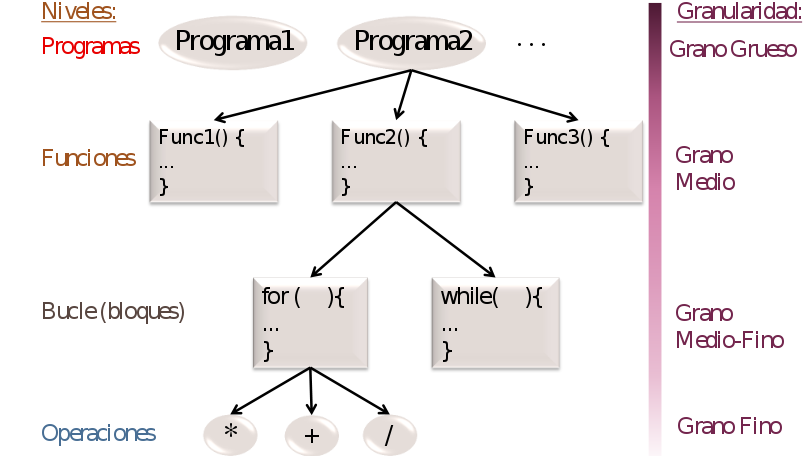
\includegraphics[width=1\textwidth]{1}
\caption{Niveles de paralelismo en el código de una aplicación y granularidad}
\label{niveles_paralelismo}
\end{figure}

Este paralelismo que se puede detectar en los niveles de un código secuencial se llama \textit{\textcolor[rgb]{0.2,0.4,0.8}{paralelismo funcional}}.

\textcolor[rgb]{0.2,0.4,0.8}{\subsection{Dependencias de datos}}
\label{dependencias_datos}
Determinan si un código puede ejecutarse en paralelo o no. Son las condiciones que se deben cumplir para que el bloque de código $B_2$ presente una dependencia de datos con respecto a $B_1$:
\begin{enumerate}[\color{azul}{\bf $\heartsuit$}]
    \item Deben hacer referencia a una misma posición de memoria M (variable)
    \item $B_1$ aparece en la secuencia de código antes que $B_2$.
\end{enumerate}

Los tipos de dependencias de datos (de $B_2$ respecto a $B_1$) son:
\begin{enumerate}[\color{azul}{\bf $\heartsuit$}]
\label{dependencias_de_datos}
    \item RAW (\textit{\textcolor[rgb]{0.2,0.4,0.8}{Read After Write}}) o dependencia verdadera: se lee el contenido de una variable después de haber escrito en esa variable. Se pretende que lo que se lee sea el resultado de lo que se ha escrito anteriormente. Si se están ejecutando a la vez puede que se ejecute la operación de lectura antes que la de escritura y que por tanto, no se lea el valor deseado.

    El siguiente código sería un ejemplo de dependencia RAW:
    \begin{minted}{c}
    ...
    a = b + c;
    d = a + c;
    ...
    \end{minted}

    Este código está hecho pensando en que primero se ejecutará \verb*|a=b+c| y después, \verb*|d=(b+c)+c|. Si lo ejecutasemos en paralelo, podríamos hacer primero \verb*|d=a+c| y luego, \verb*|a=b+c| obteniendo así, un resultado erróneo. 

    \item WAW (\textit{\textcolor[rgb]{0.2,0.4,0.8}{Write After Write}}) o dependencia de salida: el resultado de una operación se usará después en el código, y si después modificamos el valor de la variable, será porque queremos que se use después con ese valor (de hecho, los compiladores quitan el código muerto, es decir, variables que no se usan). Si ambas operaciones de escritura se ejecutan en paralelo podría ocurrir que se lea un valor incorrecto dependiendo del orden en el que se ejecuten las operaciones.

    El siguiente código sería un ejemplo de dependencia WAW:
    \begin{minted}{c}
    ...
    a = b + c;
    ...
    a = d + e;
    ...
    \end{minted}

    Primero, escribimos en la variable \verb*|a| el valor \verb*|b+c| para usar dicho valor en alguna operación siguiente. Después, volvemos a usar la variable \verb*|a| para guardar en ella otro valor distinto, \verb*|d+e| y usarlo de nuevo en cualquier otra operación. Si ejecutasemos esto en paralelo, podríamos obtener un resultado erróneo al usar en cualquier operación que espere el valor \verb*|b+c| el valor \verb*|d+e| y viceversa. Este tipo de dependencia la resuelve el compilador guardando ambos valores en registros diferentes.

    \item WAR (\textit{\textcolor[rgb]{0.2,0.4,0.8}{Write After Read}}) o antidependencia: Si ejecutamos una operación de lectura y otra de escritura posterior en paralelo, podemos escribir en la variable que se está leyendo antes de que dicha variable se lea.

    El siguiente código sería un ejemplo de dependencia WAR:
    \begin{minted}{c}
    ...
    b = a + 1;
    ...
    a = d + e;
    ...
    \end{minted}

    En primer lugar, leemos el valor de \verb*|a| y luego lo sobreescribimos. Si ejecutásemos este código en paralelo podríamos ejecutar la instrucción \verb*|b=(d+e)+1| y así, obtener un resultado erróneo. Este tipo de dependencia también la resuelve el compilador usando diferentes registros.
\end{enumerate}

Estas dependencias de datos van a limitar la paralelización. WAW y WAR se pueden eliminar cambiando el destino de salida, poniendo una variable distinta. No sólo lo hace el compilador, el hardware también lo hace. Respecto a los RAW, se pueden eliminar en alguna ocasión a nivel de bucle pero no a nivel de operación. 

Siempre que no haya dependencias RAW, podemos paralelizar las operaciones:
\begin{enumerate}[\color{azul}{\bf $\heartsuit$}]
    \item \textit{\textcolor[rgb]{0.2,0.4,0.8}{A nivel de bucle}}: pueden hacerlo los compiladores si se trata de bucles sencillos y, por supuesto, el programador.
    \item \textit{\textcolor[rgb]{0.2,0.4,0.8}{A nivel de función}}: el compilador lo tiene algo más difícil por varias razones:
    \begin{enumerate}[$\longrightarrow$]
        \item El uso de punteros
        \item El no expresar en los argumentos de la función todas las variables que se van a usar en dicha función.
        \item Si además las funciones están en ficheros distintos, tendría que entrar en acción el enlazador y dificultaría aún más la paralelización.
    \end{enumerate}
    \item \textit{\textcolor[rgb]{0.2,0.4,0.8}{A nivel de programa}}: el compilador no puede paralelizar nada porque genera código máquina para cada programa de manera independiente (no podemos compilar dos programas a la vez).
\end{enumerate}

En resumen, los compiladores extraen mejor el paralelismo a bajo nivel (granos finos) que a alto nivel, cuanto más bajo sea el nivel mejor trabajo hay. Pero este trabajo se puede superar.

\textcolor[rgb]{0.2,0.4,0.8}{\subsection{Paralelismo implícito en una aplicación}}
\textcolor[rgb]{0.2,0.4,0.8}{\subsubsection{Paralelismo de tareas}}
El \textbf{\textcolor[rgb]{0.2,0.4,0.8}{paralelismo de tareas (\textit{task-parallelism})}} se encuentra extrayendo la estructura lógica de funciones de la aplicación. En esta estructura, los bloques son funciones, y las conexiones entre ellos reflejan el flujo de datos entre funciones. Equivaldría al paralelismo a nivel de función dentro del código de alto nivel.

Se extrae la estructura lógica de las funciones en un grafo: los nodos serían las funciones y las flechas, la secuencia en la que se deberían de ejecutar. Un ejemplo de esto se ve en la \hyperref[decodificador_jpeg]{Figura \ref*{decodificador_jpeg}}

\textcolor[rgb]{0.2,0.4,0.8}{\subsubsection{Paralelismo de datos}}
El \textbf{\textcolor[rgb]{0.2,0.4,0.8}{paralelismo de datos (\textit{data-parallelism} ó \textit{DLP-Data Level Parallelism})}} se encuentra implícito en las operaciones con estructuras de datos (vectores y matrices). Se puede extraer de una representación matemática de las operaciones de la aplicación. Las operaciones con vectores y matrices engloban múltiples operaciones con datos escalares, que se pueden realizar en paralelo. Éstas operaciones se implementan mediante bucles. Por tanto, el paralelismo de datos está relacionado con el paralelismo a nivel de bucle. El paralelismo de datos se puede extraer de los bucles analizando las operaciones realizadas con la misma estructura de datos en las diferentes iteraciones del bucle.

En la década de los 90 se han ido incorporando unidades funcionales que implementan paralelismo de datos usando procesamiendo SIMD (arquitecturas multimedia). Las instrucciones multimedia aceleran el procesamiento vectorial aplicando la misma instrucción en paralelo a múltiples datos de un registro.

\textcolor[rgb]{0.2,0.4,0.8}{\subsection{Estructura de funciones lógica de una aplicación. Ej: decodificador JPEG}}

Se aplica a imagenes donde se dividen las imagenes en bloques de 8x8 píxeles. Cada cuadradito representa un bloque de 8x8 píxeles. El decodificador parte del bloque codificado y lo decodifica a través de las funciones que se indican en el grafo de la \hyperref[decodificador_jpeg]{Figura \ref*{decodificador_jpeg}}

Una vez extraída la estructura lógica de las funciones, se programarían.

\begin{figure}[!h]
\centering
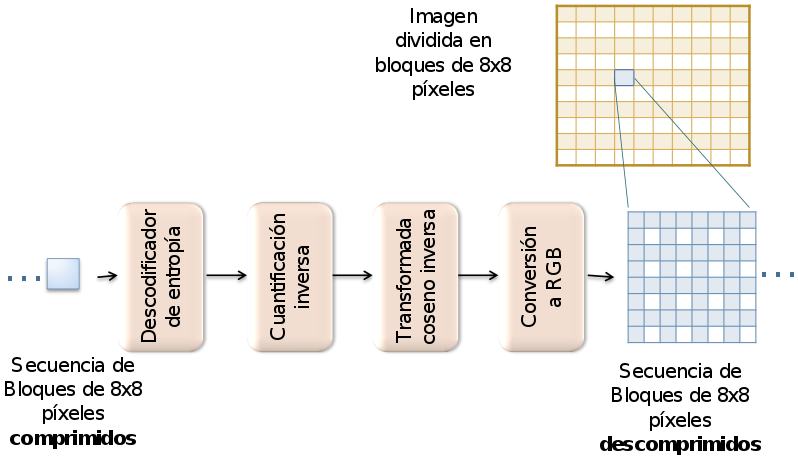
\includegraphics[width=1\textwidth]{2}
\caption{Secuencia lógica de funciones seguida por un decodificador JPEG}
\label{decodificador_jpeg}
\end{figure}

\textcolor[rgb]{0.2,0.4,0.8}{\subsection{Paralelismo de datos y paralelismo de tareas en OpenMP (Prácticas 1, 2 y 3)}}

La herramienta de prácticas permite aprovechar el paralelismo a nivel de función y bucle, pero éste debe ser extraído por el programador. En el ejemplo de la \hyperref[paralelismo_openmp]{Figura \ref*{paralelismo_openmp}}, las funciones se pueden ejecutar en paralelo, para ello se usan las directivas de la imagen. Con eso se añade lo necesario para ejecutar las funciones en paralelo. Si nos hemos equivocado y hay una función que necesita el resultado que otra produce, obtendremos resultado erróneo pero la herramienta no dirá nada. También podemos hacer esto con bucles añadiendo delante del bucle una frase y si hay dependiendias RAW obtendremos resultado erróneo, igual que antes.

\begin{figure}[!h]
\centering
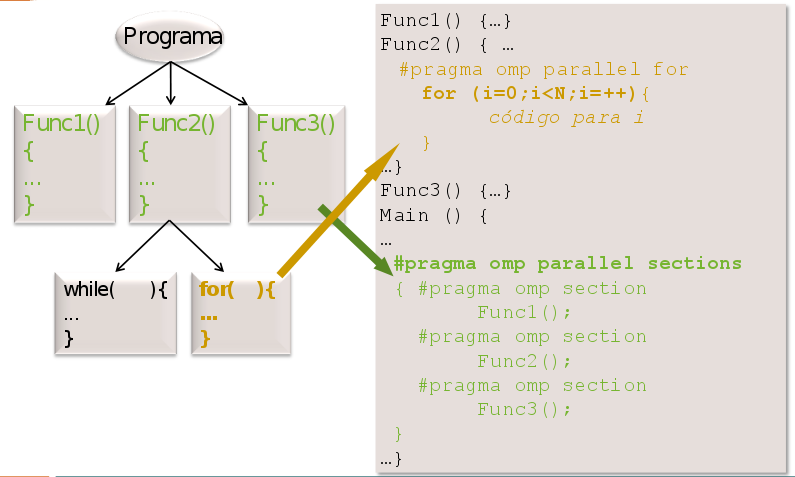
\includegraphics[width=1\textwidth]{3}
\caption{Paralelismo en OpenMP}
\label{paralelismo_openmp}
\end{figure}

\newpage
\textcolor[rgb]{0.2,0.4,0.8}{\subsection{Paralelismo implícito (nivel de detección), explícito y arquitecturas paralelas}}
En la \hyperref[paralelismo_ap]{Figura \ref*{paralelismo_ap}} se relacionan los distintos niveles en los que se encuentra el paralelismo implícito en el código, con los niveles en los que se puede hacer explícito y con arquitecturas paralelas que aprovechan el paralelismo.

El paralelismo entre programas se utiliza a nivel de procesos. En el momento en el que se ejecuta un programa, se crea el proceso asociado al programa. Este paralelismo es aprovechado por arquitecturas multicomputador y multiprocesador.

El paralelismo disponible entre funciones se puede extraer para utilizarlo a nivel de procesos o de hebras y lo aprovechan las arquitecturas multiprocesador y multithread.

El paralelismo dentro de un bucle, se puede extraer también a nivel de procesos o de hebras. Se puede aumentar la granularidad asociando un mayor número de iteraciones del ciclo a cada unidad a ejecutar en paralelo. El paralelismo dentro de un bucle también se puede hacer explícito dentro de una instrucción vectorial, es decir: instrucciones multimedia, para que sea aprovechado por arquitecturas SIMD o vectoriales.

El paralelismo entre operaciones se puede aprovechar en arquitecturas con paralelismo a nivel de instrucción ejecutando en paralelo las instrucciones asociadas a estas operaciones independientes.

% El paralelismo a nivel de operación se extrae de las instrucciones y lo aprovechan las arquitecturas ILP (segmentadas, superescalares...)

% El paralelismo a nivel de bucle se puede extraer de instrucciones multimedia que operan con vectores, es decir, de las intrainstrucciones (del interior de la instrucción, porque como hemos dicho antes las instrucciones multimedia eran capaces de ejecutar dos operaciones) y lo aprovechan las arquitecturas DLP.

% El paralelismo a nivel de función se puede extraer de los thread y lo aprovechan las arquitecturas TLP (multiprocesador, multithread)

% Por último, el paralelismo a nivel de programa sólo se puede extraer de los procesos y lo aprovechan las arquitecturas TLP (multicomputador, multiprocesador, multithread).

Una visión más general de este gráfico se ve en la \hyperref[resumen]{Figura \ref*{resumen}}


\begin{figure}[!h]
\centering
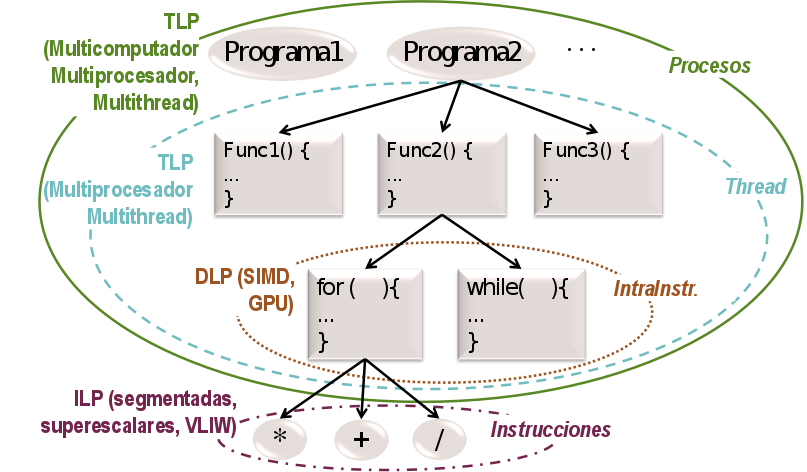
\includegraphics[width=1\textwidth]{4}
\caption{Niveles de detección en arquitecturas paralelas}
\label{paralelismo_ap}
\end{figure}

\newpage
\textcolor[rgb]{0.2,0.4,0.8}{\subsection{Nivel de paralelismo explícito. Unidades de ejecución en un computador}}
El hardware se encarga de gestionar la ejecución de instrucciones. A nivel superior, el sistema operativo se encarga de gestionar la ejecución de unidades de mayor granularidad: los procesos y hebras.

\begin{enumerate}[\color{azul}{\bf $\heartsuit$}]
    \item \textit{\textcolor[rgb]{0.2,0.4,0.8}{Instrucciones}}: la unidad de control de un core o procesador gestiona la ejecución de instrucciones por la unidad de procesamiento.
    \item \textit{\textcolor[rgb]{0.2,0.4,0.8}{Thread o light process}}: es la menor unidad de ejecución que gestiona el sistema operativo y la menor secuencia de instrucciones que se pueden ejecutar en paralelo.
    \item \textit{\textcolor[rgb]{0.2,0.4,0.8}{Proceso o process}}: es la mayor unidad de ejecución que gestiona el sistema operativo. Consta de uno o varios thread.
\end{enumerate}

\textcolor[rgb]{0.2,0.4,0.8}{\subsection{Nivel de paralelismo explícito. Thread versus procesos}}
\begin{figure}[!h]
\centering
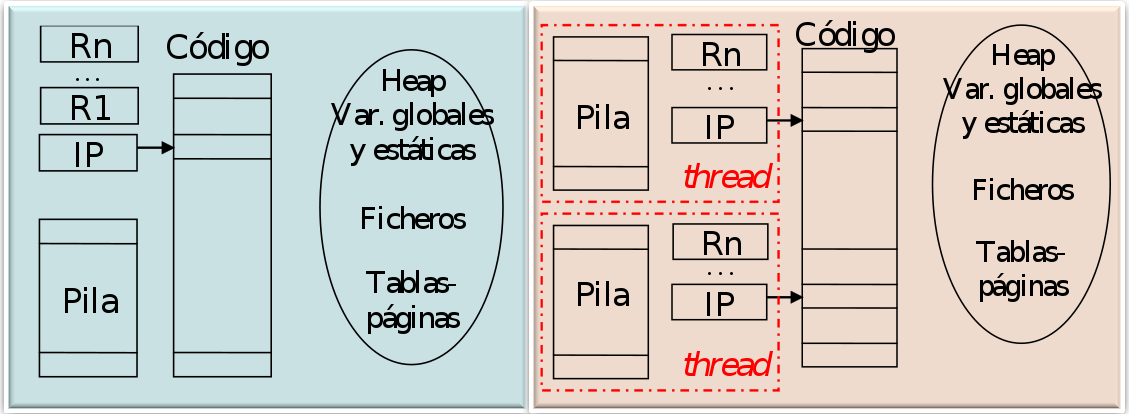
\includegraphics[width=1\textwidth]{5}
\caption{Estructura en memoria de un proceso secuencial y multihebrado}
\label{processVSthread}
\end{figure}

Cada proceso en ejecución tiene su propia asignación de memoria con todo lo que hace falta para su ejecución: datos en pila, registros, tablas de páginas y ficheros abiertos, etc. Los sistemas operativos multihebra permiten que un proceso se componga de una o varias hebras. Una hebra tiene su propia pila y contenido de registros pero comparte el código, las variables globales y otros recursos con las hebras del mismo proceso. Estas características hacen que las hebras se puedan crear y destruir en menos tiempo que los procesos, y que la comunicación, sincronización y conmutación entre hebras de un proceso sea más rápida que entre procesos. Todo ello permite que las hebras puedan tener una granularidad menor que los procesos, como se muestra en la \hyperref[granularidad_hebras]{Figura \ref*{granularidad_hebras}}.

\begin{figure}[!h]
\centering
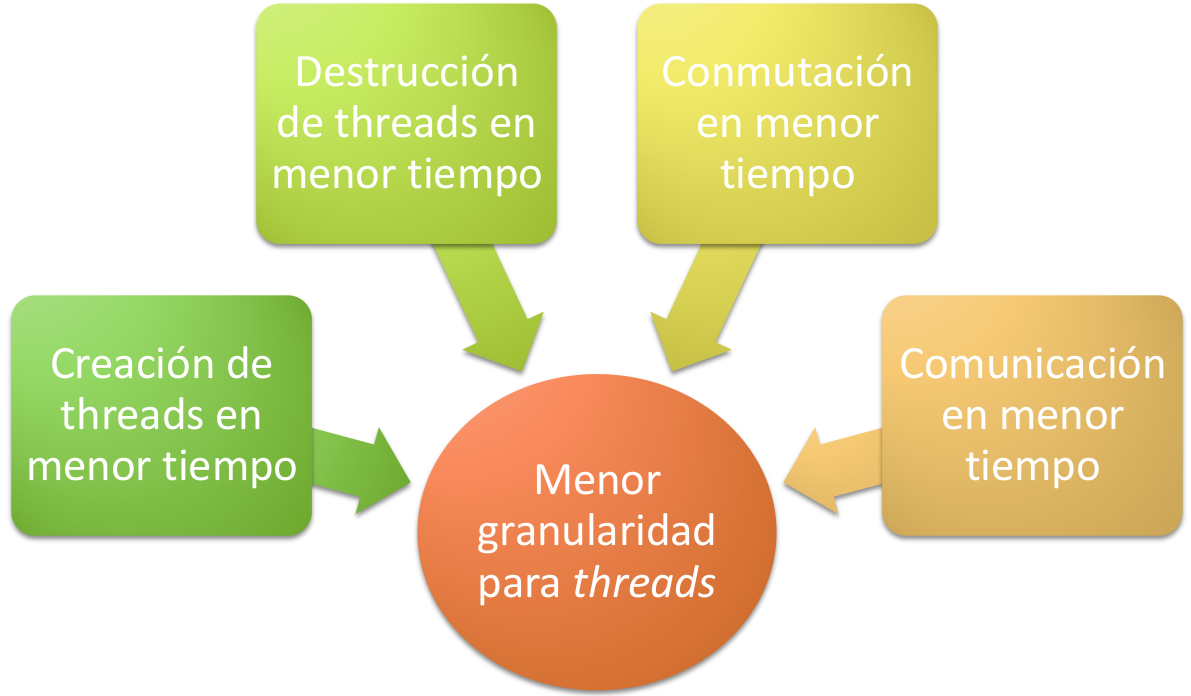
\includegraphics[width=0.7\textwidth]{6}
\caption{Razones por las que las thread tienen menor granularidad que los procesos}
\label{granularidad_hebras}
\end{figure}

Para comunicar procesos tenemos que hacer llamadas al sistema operativo que suponen una mayor sobrecarga que la comunicación entre hebras, pues ésta se realiza en la memoria que comparten.

Las diferencias entre la estructura de las hebras y de los procesos se puede ver en la \hyperref[processVSthread]{Figura \ref*{processVSthread}}.

El paralelismo implícito en el código de una aplicación se puede hacer \textit{\textcolor[rgb]{0.2,0.4,0.8}{explícito}} a nivel de instrucciones, hebras o procesos.

\textcolor[rgb]{0.2,0.4,0.8}{\subsection{Detección, utilización, implementación y extracción del paralelismo}}
\begin{figure}[!h]
\centering
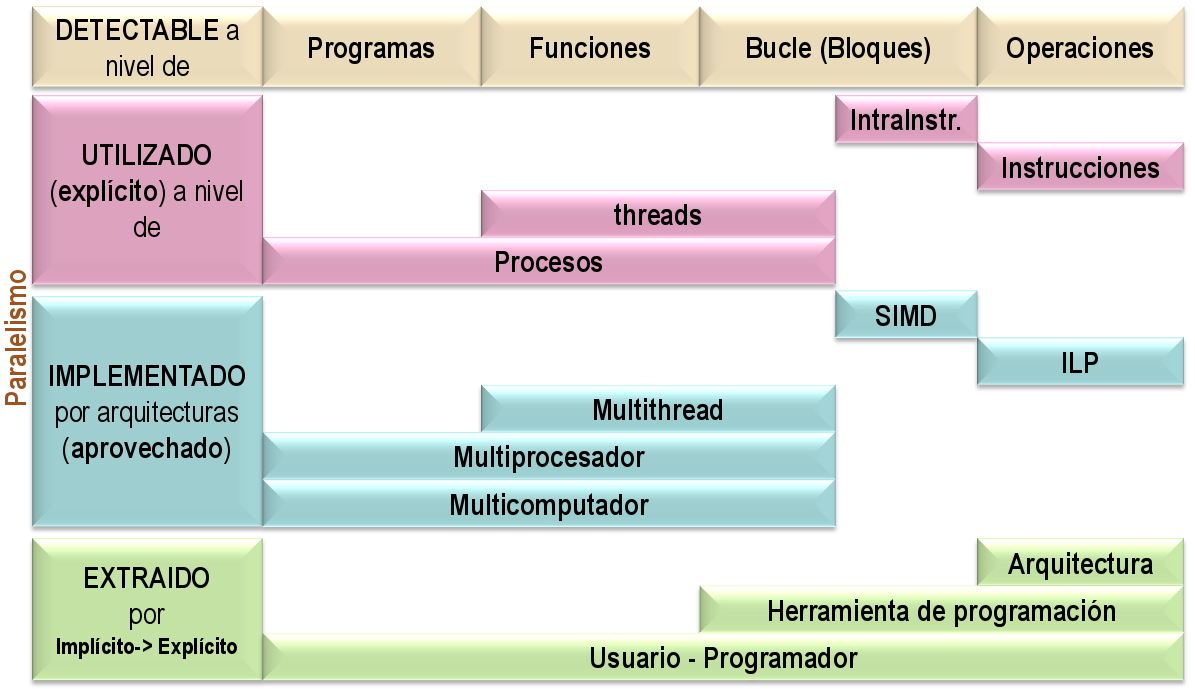
\includegraphics[width=1\textwidth]{7}
\caption{Detección, utilización, implementación y extracción del paralelismo}
\label{resumen}
\end{figure}

En la \hyperref[resumen]{Figura \ref*{resumen}} se relaciona el agente que extrae el paralelismo implícito en los diferentes niveles del código de la aplicación, con los niveles en los que se hace explícito y las arquitecturas que lo aprovechan.

En los procesadores ILP (superescalares o segmentados) la arquitectura \textit{\textcolor[rgb]{0.2,0.4,0.8}{extrae}} paralelismo. Para ello, eliminan dependencias de datos falsas entre instrucciones y evitan problemas debidos a dependencias de datos, de control y de recursos (columna 4). El \textit{\textcolor[rgb]{0.2,0.4,0.8}{grado de paralelismo}}\footnote{Podemos definir el grado de paralelismo de un conjunto de entradas a un sistema como el máximo número de entradas del conjunto que se puede ejecutar en paralelo, este número será menor al número de entradas debido a las dependencias} de las instrucciones aprovechado puede aumentar con la ayuda del compilador (herramienta de programación) y del programador.

Hay compiladores que extraen el paralelismo de datos implícito a nivel de bucle (columna 3). Algunos compiladores lo hacen explícito a nivel de hebra y otros dentro de una instrucción para que se pueda aprovechar en arquitecturas SIMD o vectoriales.

Aún es difícil para un compilador extraer paralelismo a nivel de función sin la ayuda del programador. El programador puede extraer el paralelismo implícito en un bucle o entre funciones definiendo hebras y/o procesos (columnas 2 y 3).

La distribución de las tareas independientes entre hebras y procesos dependerá:
\begin{enumerate}[\color{azul}{\bf $\heartsuit$}]
    \item de la granularidad de las unidades de código independientes
    \item de la posibilidad que ofrezca la herramienta de programación paralela disponible de definir hebras o procesos
    \item de la arquitectura disponible para aprovechar el paralelismo
    \item del sistema operativo disponible
\end{enumerate}

Los usuarios del sistema al ejecutar programas están creando procesos que se pueden ejecutar en el sistema o bien concurrentemente, o bien en paralelo (columna 1).

\newpage
\textcolor[rgb]{0.2,0.4,0.8}{\section{Clasificación de arquitecturas paralelas}}
\textcolor[rgb]{0.2,0.4,0.8}{\subsection{Computación paralela --- Computación distribuida}}
\begin{description}
  \item[Computación paralela]: estudia los aspectos hardware y software relacionados con el desarrollo y ejecución de aplicaciones en un sistema de cómputo compuesto por \textbf{\textcolor[rgb]{0.2,0.4,0.8}{múltiples procesadores/cores/computadores}} que es visto externamente como una \textbf{\textcolor[rgb]{0.2,0.4,0.8}{unidad autónoma}} (multicores, multiprocesadores, multicomputadores, cluster\footnote{Los cluster son computadores paralelos basados en computadores (nodos) y redes disponibles comercialmente, lo que les permite ser los sistemas con mejor relación prestaciones/coste en los diferentes niveles del mercado en los que se encuentran}).

  El paralelismo en las arquitecturas se ha implementado siguiendo dos líneas fundamentales: \textit{\textcolor[rgb]{0.2,0.4,0.8}{replicación de elementos}} entre los que se distribuye el trabajo y la \textit{\textcolor[rgb]{0.2,0.4,0.8}{segmentación de cauce}} técnica que divide un elemento en una serie de etapas que funcionan de manera independiente y por las que van pasando instrucciones, operandos, etc.

  \item[Computación distribuida]: estudia los aspectos hardware y software relacionados con el desarrollo y ejecución de aplicaciones en un \textbf{\textcolor[rgb]{0.2,0.4,0.8}{sistema distribuido}}; es decir, en una \textbf{\textcolor[rgb]{0.2,0.4,0.8}{colección de recursos autónomos}} (PC, servidores de datos, aplicaciones, supercomputadores...) situados en \textbf{\textcolor[rgb]{0.2,0.4,0.8}{distintas localizaciones físicas}}
\begin{figure}[!h]
\centering
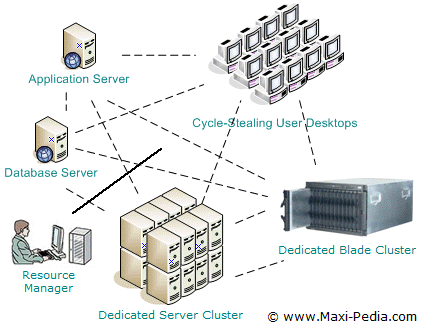
\includegraphics[width=0.6\textwidth]{9}
\caption{El concepto de computación distribuida es simple: reunir y emplear todos los recursos posibles para acelerar la computación.}
\label{dist_computing}
\end{figure}
\end{description}

\textcolor[rgb]{0.2,0.4,0.8}{\subsection{Computación distribuida a gran escala: Computación grid}}
\begin{description}
  \item[Computación distribuida a baja escala]: estudia los aspectos relacionados con el desarrollo y ejecución de aplicaciones en una colección de recursos autónomos \textbf{\textcolor[rgb]{0.2,0.4,0.8}{de un dominio administrativo}} situados en \textbf{\textcolor[rgb]{0.2,0.4,0.8}{distintas localizaciones físicas}} conectados a través de \textbf{\textcolor[rgb]{0.2,0.4,0.8}{infrastructura de red local}}.
  \item[Computación grid]: estudia los aspectos relacionados con el desarrollo y ejecución de aplicaciones en una colección de recursos autónomos de \textbf{\textcolor[rgb]{0.2,0.4,0.8}{múltiples dominios administrativos geográficamente distribuidos}} conectados con \textbf{\textcolor[rgb]{0.2,0.4,0.8}{infraestructura de telecomunicaciones}}

La computación grid virtualiza los recursos de procesamiento de múltiples ordenadores para usarlos en resolver un único problema, ya sea a través de hardware dedicado o compartido. Lo que esto significa es que tu aplicación grid no está ``atada'' a tu ordenador, sino que puede usar más de un ordenador y otros recursos más allá de tus paredes para mejorar su rendimiento.


\begin{figure}[!h]
\centering
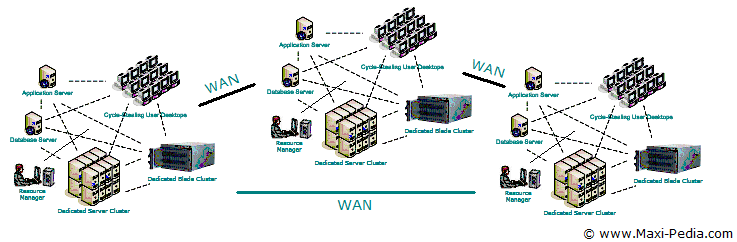
\includegraphics[width=1\textwidth]{8}
\caption{La computación grid no sólo emplea recursos sino sistemas enteros de varias localizaciones mientras cruzan límites geográficos y políticos}
\label{grid_computing}
\end{figure}


\end{description}

La clave para distinguir la computación grid y la computación distribuida está en la manera en la que se gestionan los recursos. La computación distribuida usa un gestor de recursos centralizado y todos los nodos trabajan juntos como un sistema unificado. La computación grid utiliza una estructura donde cada nodo tiene su propio gestor de recursos y el sistema no actúa como una sola unidad.

\textcolor[rgb]{0.2,0.4,0.8}{\subsection{Computación distribuida a gran escala: Computación nuble o cloud}}
La \textit{\textcolor[rgb]{0.2,0.4,0.8}{computación cloud}} comprende los aspectos relacionados con el desarrollo y ejecución de aplicaciones en un \textit{\textcolor[rgb]{0.2,0.4,0.8}{sistema cloud}}.


\textcolor[rgb]{0.2,0.4,0.8}{\subsubsection{Sistema cloud}}
Ofrece \textbf{\textcolor[rgb]{0.2,0.4,0.8}{servicios}} de \textbf{\textcolor[rgb]{0.2,0.4,0.8}{infraestructura}} (Ej: una máquina), \textbf{\textcolor[rgb]{0.2,0.4,0.8}{plataforma}} (Ej: una máquina con un sistema operativo y un software) y/o \textbf{\textcolor[rgb]{0.2,0.4,0.8}{software}} (Ej: Dropbox), por los que se paga cuando se necesitan (\textit{\textcolor[rgb]{0.2,0.4,0.8}{pay-per-use}}) y a los que se accede típicamente a través de una \textbf{\textcolor[rgb]{0.2,0.4,0.8}{interfaz (web) de auto-servicio}}.

Consta de \textbf{\textcolor[rgb]{0.2,0.4,0.8}{recursos virtuales}} que:
\begin{enumerate}[\color{azul}{\bf $\heartsuit$}]
  \item Son una \textit{\textcolor[rgb]{0.2,0.4,0.8}{abstracción}} de los recursos físicos.
  \item Parecen \textit{\textcolor[rgb]{0.2,0.4,0.8}{ilimitados}} en número y capacidad y son reclutados/liberados de forma inmediata sin interacción con el proveedor.
  \item Soportan el acceso de múltiples clientes (\textit{\textcolor[rgb]{0.2,0.4,0.8}{multitenant}}).
  \item Están conectados con métodos \textbf{\textcolor[rgb]{0.2,0.4,0.8}{estándar independientes}} de la plataforma de acceso.
\end{enumerate}

\textcolor[rgb]{0.2,0.4,0.8}{\subsection{Criterios de clasificación de computadores}}
\begin{enumerate}[\color{azul}{\bf $\heartsuit$}]
\item \textbf{\textcolor[rgb]{0.2,0.4,0.8}{Comercial}}: el \textit{\textcolor[rgb]{0.2,0.4,0.8}{grado de accesibilidad}} al hardware depende en gran medida de su precio de la accesibilidad del software. El precio no sólo depende del \textit{\textcolor[rgb]{0.2,0.4,0.8}{coste de diseño}} y del \textit{\textcolor[rgb]{0.2,0.4,0.8}{coste de fabricación}}, también del \textit{\textcolor[rgb]{0.2,0.4,0.8}{volumen de venta}} y de la \textit{\textcolor[rgb]{0.2,0.4,0.8}{competencia}}. El grado de accesibilidad al software depende de factores como el coste de desarrollo, volumen de venta y competencia.
\begin{enumerate}[$\longrightarrow$]
\item \textbf{\textcolor[rgb]{0.2,0.4,0.8}{Segmento de mercado}}: Los sistemas con múltiples procesadores pueden encontrarse en los diferentes niveles del mercado de computadores.
% \begin{itemize}
%   \item Supercomputadores
%   \item Servidores de alta gama (\$$500.000 <$ \textit{\textcolor[rgb]{0.2,0.4,0.8}{high-end}})
%   \item Servidores de gama media (\$$25.000 <$ \textit{\textcolor[rgb]{0.2,0.4,0.8}{mid-range}} $<$ \$$500.000$)
%   \item Servidores de gama baja (\textit{\textcolor[rgb]{0.2,0.4,0.8}{entry-level}} $<$ \$$25.000$)
%   \item PC/WS
%   \item Mercado de computadores empotrados
% \end{itemize}

\begin{figure}[!h]
\centering
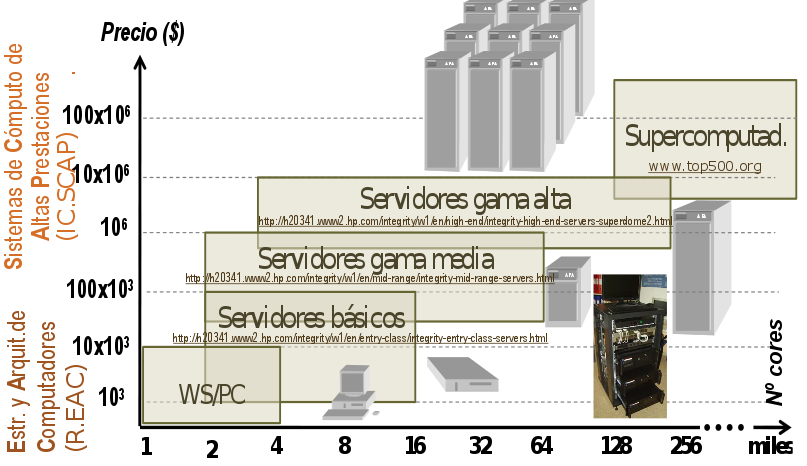
\includegraphics[width=1\textwidth]{10}
\caption{Clasificación del mercado de sistemas con múltiples procesadores}
\label{grafica_mercado}
\end{figure}

La \hyperref[grafica_mercado]{clasificación \ref*{grafica_mercado}} se ha hecho teniendo en cuenta la clasificación que hacen los propios vendedores con sus sistemas, el precio del sistema y la clasificación de servidores en función de su precio IDC (\textit{\textcolor[rgb]{0.2,0.4,0.8}{International Data Corporation}}). Conforme se baja de nivel disminuyen el precio y las prestaciones por unidad, y aumenta el volumen de ventas. El precio en un nivel del mercado depende del número de procesadores que incluye el sistema y del grado de utilización de componentes disponibles comercialmente ya que al tener mayor volumen de venta tienen el precio más bajo.

En el nivel más bajo están los sistemas empotrados, que se hacen para un propósito específico. Tienen restricciones de consumo de potencia, precio, tamaño y tiempo real, presentan dificultades para el programador pues tiene que programar eficientemente limitándose por un procesador más malo, un determinado consumo de potencia, etc para sacar partido máximo a la arquitectura. Después, los PC y estaciones de trabajo que  se hacen para todo tipo de aplicaciones y generalmente tienen un procesador. El precio más alto de estos computadores es \$$10.000$. El precio más alto se corresponde con estaciones de trabajo SMP y el más bajo con PCs de baja gama.

En los siguientes niveles nos encontramos los \textbf{\textcolor[rgb]{0.2,0.4,0.8}{servidores}}. IDC clasifica los servidores en tres grupos en función de su precio.
\begin{itemize}
  \item servidores básicos (\textit{\textcolor[rgb]{0.2,0.4,0.8}{entry-level}} ó \textit{\textcolor[rgb]{0.2,0.4,0.8}{volume servers}}): incluyen aquellos con un precio inferior a \$$25.000$. 
  \item servidores de gama media (\textit{\textcolor[rgb]{0.2,0.4,0.8}{mid-range}}): con precios entre \$$25.000$ y \$$500.000$
  \item servidores de gama alta (\textit{\textcolor[rgb]{0.2,0.4,0.8}{high-end}}): con precios mayores a \$$500.000$
\end{itemize}

Por último, se ha tomado como un grupo aparte de servidores de alta gama los \textbf{\textcolor[rgb]{0.2,0.4,0.8}{supercomputadores}}. Esta denominación se asigna a los computadores que ofrecen mayores prestaciones, siendo también los de mayor coste y prestaciones. Dado su precio, tienen el grado de accesibilidad más bajo. El criterio utilizado para clasificar los supercomputadores son las prestaciones que ofrece el benchmark LINPACK\footnote{este benchmark ofrece una medida de la velocidad con la que la máquina ejecuta instrucciones de punto flotante.}

% Los tres primeros son \textcolor[rgb]{0.2,0.4,0.8}Sistemas de \textcolor[rgb]{0.2,0.4,0.8}Cómputo de \textcolor[rgb]{0.2,0.4,0.8}Altas \textcolor[rgb]{0.2,0.4,0.8}Prestaciones (IC.SCAP). Los servidores de gama baja y los PC son \textcolor[rgb]{0.2,0.4,0.8}Estructura y \textcolor[rgb]{0.2,0.4,0.8}Arquitectura de \textcolor[rgb]{0.2,0.4,0.8}Computadores (R.EAC) y, los computadores empotrados, \textcolor[rgb]{0.2,0.4,0.8}Sistemas de \textcolor[rgb]{0.2,0.4,0.8}Cómputo para \textcolor[rgb]{0.2,0.4,0.8}Aplicaciones \textcolor[rgb]{0.2,0.4,0.8}Específicas (IC.SCAE)


\end{enumerate}
\item \textbf{\textcolor[rgb]{0.2,0.4,0.8}{Educación, investigación (también usados por fabricantes y vendedores)}}:
\begin{enumerate}[$\longrightarrow$]
\begin{figure}[!h]
\centering
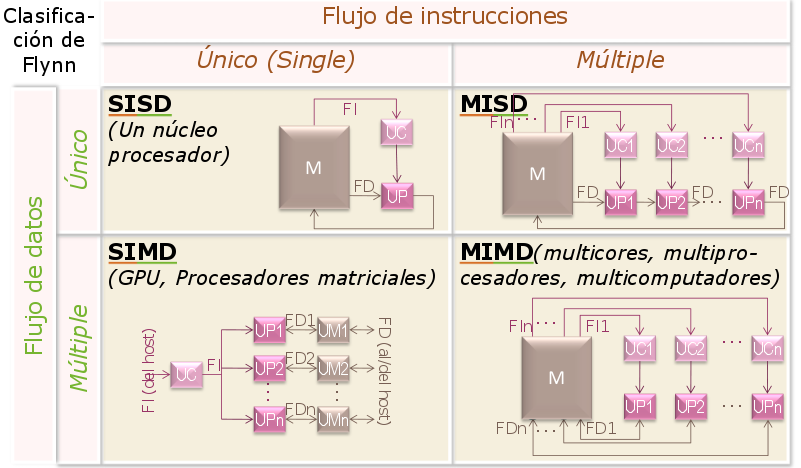
\includegraphics[width=1\textwidth]{11}
\caption{Clases de computadores en la taxonomía de Flynn: según el número de instrucciones y datos. M = memoria principal, UC = unidad de control, UP = unidad de procesamiento.}
\label{flynn}
\end{figure}
\item \textbf{\textcolor[rgb]{0.2,0.4,0.8}{Flujos de control y flujos de datos: clasificación de Flynn (1972)}}: esta clasificación (\hyperref[flynn]{Figura \ref*{flynn}}) divide los computadores en cuatro clases según el número de secuencias o flujos de instrucciones y secuencias o flujos de datos que pueden procesarse simultáneamente en el computador:
\begin{itemize}
\item \textit{\textcolor[rgb]{0.2,0.4,0.8}{Computadores SISD}}: un único flujo de instrucciones (SI, \textit{\textcolor[rgb]{0.2,0.4,0.8}{Single Instruction}}) procesa operandos y genera resultados, definiendo un único flujo de datos (SD, \textit{\textcolor[rgb]{0.2,0.4,0.8}{Single Data}}).
\item \textit{\textcolor[rgb]{0.2,0.4,0.8}{Computadores SIMD}}: un único flujo de instrucciones (SI) procesa datos y genera resultados, definiendo varios flujos de datos (MD, \textit{\textcolor[rgb]{0.2,0.4,0.8}{Multiple Data}}), cada flujo de instrucciones ejecuta las mismas instrucciones pero las aplica sobre datos diferentes.
\item \textit{\textcolor[rgb]{0.2,0.4,0.8}{Computadores MIMD}}: el computador ejecuta varias secuencias o flujos distintos de instrucciones (MI, \textit{\textcolor[rgb]{0.2,0.4,0.8}{Multiple Instructions}}), y cada uno de ellos procesa operandos y genera resultados definiendo un único flujo de instrucciones, de forma que también existen varios flujos de datos (MD) uno por cada flujo de instrucciones.
\item \textit{\textcolor[rgb]{0.2,0.4,0.8}{Computadores MISD}}: se ejecutan varios flujos distintos de instrucciones (MI) aunque todos actúan sobre el mismo flujo de datos (SD).
\end{itemize}
\end{enumerate}
\item \textbf{\textcolor[rgb]{0.2,0.4,0.8}{Sistema de memoria}}: generalmente, los sistemas con múltiples procesadores o multiprocesadores se han clasificado atendiendo a la organización del sistema de memoria. Los sistemas de paralelismo de alto nivel se han clasificado en dos grupos:
\begin{enumerate}[$\longrightarrow$]
  \item \textbf{\textcolor[rgb]{0.2,0.4,0.8}{Sistemas con memoria compartida (SM, \textit{Shared Memory})}} ó \textbf{\textcolor[rgb]{0.2,0.4,0.8}{multiprocesadores}}: todos los procesadores comparten el mismo espacio de direcciones. El programador no necesita conocer dónde están almacenados los datos.
  \item \textbf{\textcolor[rgb]{0.2,0.4,0.8}{Sistemas con memoria distribuida (DM \textit{Distributed Memory})}} ó \textbf{\textcolor[rgb]{0.2,0.4,0.8}{multicomputador}}: cada procesador tiene su propio espacio de direcciones particular. El programador necesita conocer dónde están almacenados los datos.
\end{enumerate}
\item \textbf{\textcolor[rgb]{0.2,0.4,0.8}{Flujos de control (propuesta de clasificación de arquitecturas con múltiples flujos de control)}}: cuando hablamos de flujos de control nos referimos a threads (\hyperref[clasificacion_threads]{Figura \ref*{clasificacion_threads}}). Estas arquitecturas permiten paralelismo a nivel de thread sea real o concurrente y tiene dos categorías:
\begin{enumerate}[$\longrightarrow$]
\item \textbf{\textcolor[rgb]{0.2,0.4,0.8}{Implícito}}: flujos de control gestionados por la arquitectura
\item \textbf{\textcolor[rgb]{0.2,0.4,0.8}{Explícito}}: flujos de control creados y gestionados por el sistema operativo, o bien con una instancia del sistema operativo (multiprocesadores, multicores, cores multithread...) ó con múltiples instancias del sistema operativo (multicomputadores).
\end{enumerate}
\item \textbf{\textcolor[rgb]{0.2,0.4,0.8}{Nivel de paralelismo aprovechado (propuesta de clasif.)}}: Esta clasificación se divide en:
\begin{enumerate}[$\longrightarrow$]
\item \textbf{\textcolor[rgb]{0.2,0.4,0.8}{Arquitecturas con \textit{Data Level Parallelism}}}: ejecutan las operaciones de instrucción concurrentemente o en paralelo. Son unidades funcionales vectoriales o SIMD.
\item \textbf{\textcolor[rgb]{0.2,0.4,0.8}{Arquitecturas con \textit{Instruction Level Parallelism}}}: ejecutan múltiples instrucciones concurrentemente o en paralelo. Son los cores escalares segmentados, superescalares o VLIW/EPIC.
\item \textbf{\textcolor[rgb]{0.2,0.4,0.8}{Arquitecturas con \textit{Thread Level Parallelism} explícito y una instancia del SO}}: ejecutan múltiples flujos de control concurrentemente o en paralelo. Los hay de dos tipos
\begin{itemize}
   \item Cores que modifican la arquitectura escalar segmentada, superescalar o VLIW/EPIC para ejecutar threads concurrentemente o en paralelo
   \item Multiprocesadores: ejecutan threads en paralelo en un computador con múltiples cores (incluye multicores).
 \end{itemize}
 \item \textbf{\textcolor[rgb]{0.2,0.4,0.8}{Arquitectura con \textit{Thread Level Parallelism} explícito y múltiples instancias del SO}}: ejecutan múltiples flujos de control en paralelo. Son los multiprocesadores que ejecutan threads en paralelo en un sistema con múltiples computadores.
\end{enumerate}
\end{enumerate}

\begin{figure}
\centering
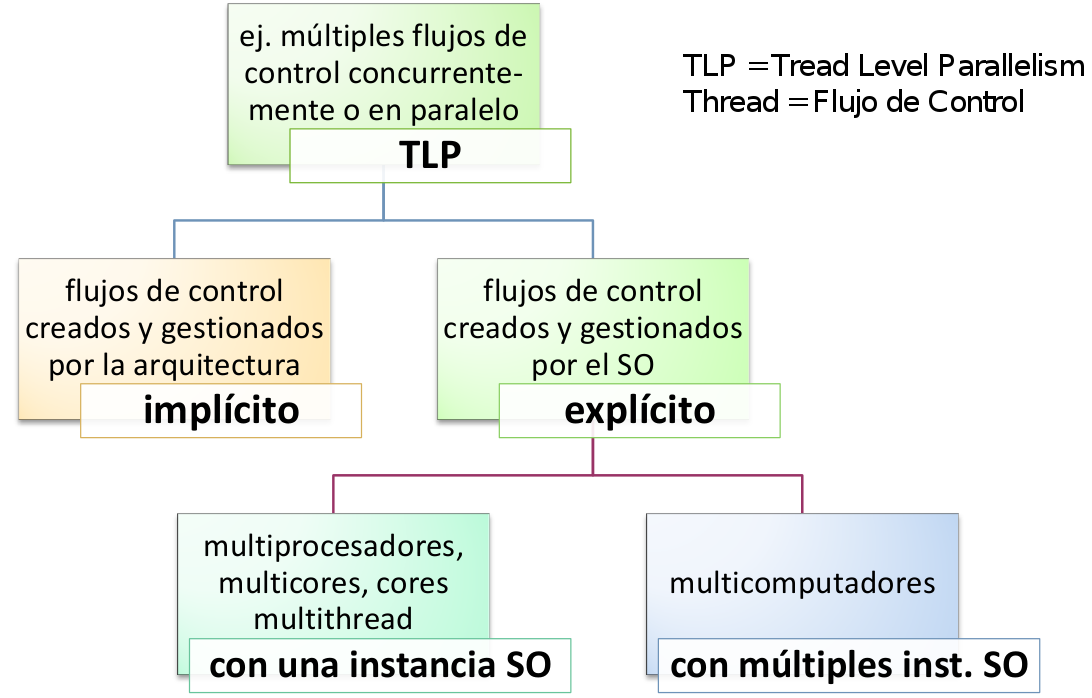
\includegraphics[width=1\textwidth]{22}
\caption{Clasificación de arquitecturas con múltiples threads}
\label{clasificacion_threads}
\end{figure}

\textcolor[rgb]{0.2,0.4,0.8}{\subsection{Computadores SISD}}
En un computador (\hyperref[sisd]{Figura \ref*{sisd}}) SISD existe una única unidad de control (UC) que recibe las instrucciones de memoria, las decodifica y genera los códigos que definen la operación correspondiente a cada instrucción que debe realizar la unidad de procesamiento (UP) de datos. El flujo de datos se establece a partir de los operandos necesarios para realizar la operación codificada en cada instrucción, que se traen desde memoria, y de los resultados generados por las instrucciones que se almacenan en memoria. Se corresponde a computadores uniprocesador. 

% \newpage
El siguiente código:

\begin{minted}{pascal}
for i:=1 to 4 do
begin
    C[i]:=A[i]+B[i];
    F[i]:=D[i]-E[i];
    G[i]:=K[i]*H[i];
end;
\end{minted}

Implica realizar doce operaciones, más las correspondientes al control del bucle. Una ejecución del código anterior en un SISD precisaría doce intervalos de tiempo.

\begin{figure}[!h]
\centering
\mbox {
\subfigure[Descripción estructural]{
\label{estructura_sisd}
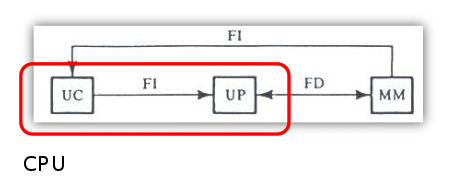
\includegraphics[width=0.4\textwidth]{12}
}
\qquad
\subfigure[Descripción funcional] {
\label{funcion_sisd}
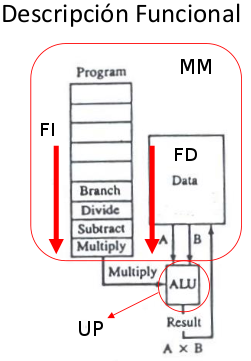
\includegraphics[width=0.2\textwidth]{13}
}
}
\caption{Descripción de un computador SISD}
\label{sisd}
\end{figure}


\textcolor[rgb]{0.2,0.4,0.8}{\subsection{Computadores SIMD}}
En un computador SIMD (\hyperref[simd]{Figura \ref*{simd}}) los códigos que genera la única unidad de control del computador a partir de cada instrucción actúan sobre varias unidades de procesamiento distintas (UP$_i$). Así, se pueden realizar varias operaciones similares simultáneas con operandos distintos. Cada una de las secuencias de operandos y resultados utilizados por las distintas unidades de proceso define un flujo de datos diferente. Aprovechan el \textbf{\textcolor[rgb]{0.2,0.4,0.8}{paralelismo de datos}}.

El siguiente código:
\begin{minted}{pascal}
for all EPi(i:=1 to 4) do
begin
        C[i]:=A[i]+B[i];
        F[i]:=D[i]-E[i];
        G[i]:=K[i]*H[i];
end;
\end{minted}

Correspondería a un procesador matricial con cuatro unidades de proceso (UP$_i$, $i=1,\cdots,4$). En este caso, se necesitarían tres intervalos de tiempo. Es decir, cuatro veces menos que en el computador SISD, teniendo en cuenta que se están incluyendo cuatro unidades de proceso, tal y como se ve en la \hyperref[procesador_matricial]{Figura \ref*{procesador_matricial}}

\begin{figure}[!h]
\centering
\mbox {
\subfigure[Descripción estructural]{
\label{estructura_sisd}
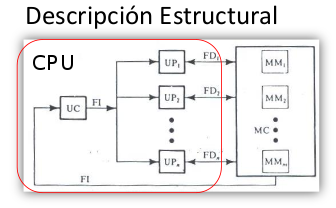
\includegraphics[width=0.4\textwidth]{14}
}
\qquad
\subfigure[Descripción funcional] {
\label{funcion_sisd}
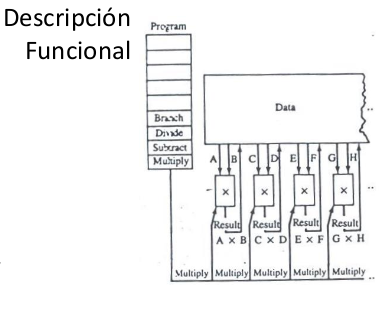
\includegraphics[width=0.35\textwidth]{15}
}
}
\caption{Descripción de un computador SIMD}
\label{simd}
\end{figure}

\begin{figure}[!h]
\centering
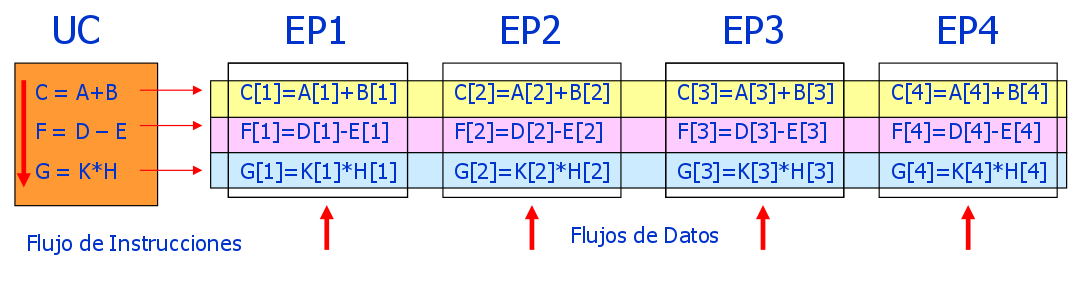
\includegraphics[width=1\textwidth]{19}
\caption{Procesador matricial}
\label{procesador_matricial}
\end{figure}

También tenemos procesadores vectoriales, que simulan el paralelismo ejecutando las instrucciones concurrentemente, es decir, todas las instrucciones usan el mismo recurso, no como en el matricial que hay una réplica del recurso y cada instrucción usa una. Los procesadores vectoriales se dividen en etapas (se podría decir que están segmentados) y en cada etapa del segmento se va calculando una suma diferente. El esquema de un procesador vectorial se representa en la \hyperref[procesador_vectorial]{Figura \ref*{procesador_vectorial}}

\begin{figure}[!h]
\centering
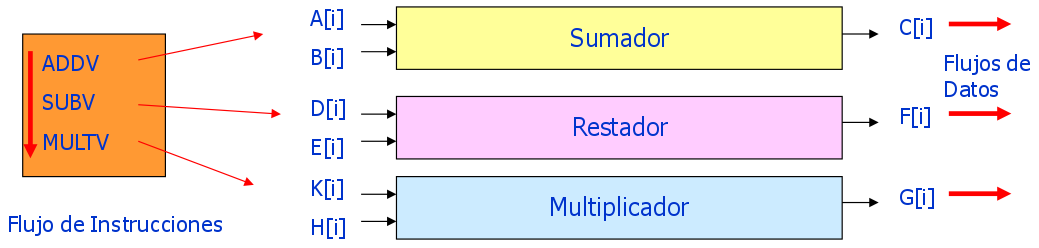
\includegraphics[width=1\textwidth]{21}
\caption{Procesador vectorial}
\label{procesador_vectorial}
\end{figure}

\textcolor[rgb]{0.2,0.4,0.8}{\subsection{Computadores MIMD}}
En un computador MIMD (\hyperref[mimd]{Figura \ref*{mimd}}) existen varias unidades de control que decodifican las instrucciones correspondientes a distintos programas. Cada uno de esos programas procesa conjuntos de datos diferentes, que definen distintos flujos de datos. Corresponde con multinúcleos, multiprocesadores y multicomputadores: puede aprovechar, además, \textbf{\textcolor[rgb]{0.2,0.4,0.8}{paralelismo funcional}}.

En los computadores MIMD, para ejecutar los códigos anteriores se consideran tres procesadores (Proc1, Proc2 y Proc3) y cada uno ejecuta una operación distinta con los cuatro componentes de los distintos vectores:
\begin{minted}{pascal}
for i:=1 to 4 do        for i:=1 to 4 do        for i:=1 to 4 do
begin                   begin                   begin
    C[i]:=A[i]+B[i];        F[i]:=D[i]-E[i];        G[i]:=K[i]*H[i];
end;                    end;                    end;
Proc 1                  Proc 2                  Proc 3
\end{minted}

En este caso, el coste temporal sería de 4 unidades de tiempo: tres veces menos que en la implementación secuencial. 

También se podría usar un MIMD con cuatro procesadores en el que cada uno realizaría las tres operaciones con una de las cuatro componentes de los vectores. En este caso, el tiempo se reduciría a cuatro intervalos de tiempo, cuatro veces menos que en el caso de un SISD. En esta situación se dice que el computador MIMD utiliza una implementación SPMD (\textit{\textcolor[rgb]{0.2,0.4,0.8}{Single Program Multiple Data}}) del problema.

\begin{figure}[!h]
\centering
\mbox {
\subfigure[Descripción estructural]{
\label{estructura_sisd}
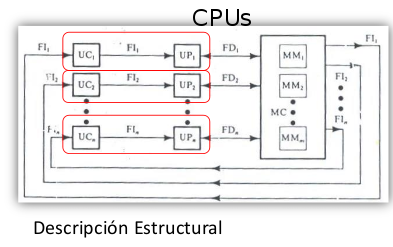
\includegraphics[width=0.4\textwidth]{16}
}
\qquad
\subfigure[Descripción funcional] {
\label{funcion_sisd}
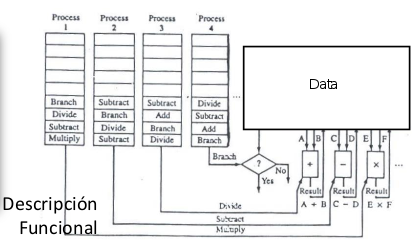
\includegraphics[width=0.45\textwidth]{17}
}
}
\caption{Descripción de un computador MIMD}
\label{mimd}
\end{figure}

\textcolor[rgb]{0.2,0.4,0.8}{\subsection{Computadores MISD}}
Los computadores MISD (\hyperref[misd]{Figura \ref*{misd}}) constituyen una clase de computadores cuyo comportamiento se puede implementar con iguales prestaciones en un computador MIMD en el que sus procesadores se sincronizan para que los datos vayan pasando desde un procesador a otro. Por eso, si bien se pueden identificar computadores de las demás clases (SISD, SIMD...) no existen computadores MISD específicos. Si la forma de procesamiento MISD es provechosa para algún problema, éste se puede implementar en un computador MIMD en el que los datos son procesados sucesivamente por los procesadores del sistema.

\begin{figure}[!h]
\centering
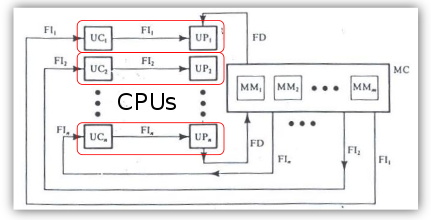
\includegraphics[width=0.6\textwidth]{18}
\caption{Descripción estructural de un computador MISD}
\label{misd}
\end{figure}

\textcolor[rgb]{0.2,0.4,0.8}{\subsection{Comparativa SMP (Symmetric Multi-Processor) y Multicomputadores y comunicación entre procesadores}}
En un multicomputador, la memoria asignada a un procesador se encuentra ubicada cerca del procesador. En un multiprocesador, toda la memoria se encuentra situada a igual distancia de todos los procesadores y físicamente enlazada. 

En un multicomputador cada procesador tiene su propio espacio de direcciones, es por tanto lógico que en su estructura física, cerca de cada procesador haya un módulo de memoria local, en el que se encuentre su espacio de direcciones. También nos podemos encontrar distribuido el sistema de E/S. En un multiprocesador, todos los procesadores comparten el mismo espacio de direcciones por tanto, la estructura física para multiprocesadores tiene los módulos de memoria ubicados en la misma zona del sistema, separados de los procesadores por una red de conexión que arbitre el acceso a los módulos. También nos podemos encontrar centralizados los dispositivos de E/S. 

Con esta estructura, el tiempo de acceso de los procesadores a memoria (se puede extender también a los dispositivos de E/S), será igual sea cual sea la posición de memoria a la que acceden, es una estructura simétrica. Los multiprocesadores con esta característica se denominan SMP (\textit{\textcolor[rgb]{0.2,0.4,0.8}{Symmetric Multi-Processor}}) o \textit{\textcolor[rgb]{0.2,0.4,0.8}{multiprocesadores simétricos}}. El acceso a memoria se realiza a través de la red de interconexión.

En multicomputadores, cada procesador tiene su propio módulo de memoria local al que puede acceder directamente. En esta configuración la red de interconexión se utiliza para la transferencia de datos compartidos (mensajes) entre nodos de la red. El tamaño de los mensajes a transferir depende del programador. En un multiprocesador, el tamaño de las transferencias con memoria depende del hardware, y será menor que el de las transferencias entre nodos en un multicomputador. 

El comportamiento de ambos ante diferentes facetas es:
\begin{description}
\item[Latencia en el acceso a memoria]: el tiempo de acceso a memoria es mayor en los multiprocesadores que en los multicomputadores. Esta mayor latencia se debe a:
\begin{enumerate}[\color{azul}{\bf $\heartsuit$}]
\item \textbf{\textcolor[rgb]{0.2,0.4,0.8}{La no localidad de los módulos de memoria}}, en un multicomputador cada procesador tiene su espacio de direcciones en un módulo de memoria situado en su proximidad mientras que en multiprocesadores todos los módulos de memoria están separados de los procesadores.
\item \textbf{\textcolor[rgb]{0.2,0.4,0.8}{La necesidad de acceder a memoria atravesando la red de interconexión}}
\item \textbf{\textcolor[rgb]{0.2,0.4,0.8}{El incremento en la latencia media debido a conflictos en la red entre accesos de diferentes procesadores}}, ya que si varios procesadores en un momento dado necesitan utilizar el mismo recurso, tendrán que esperar a que quede libre y esto supone una penalización en la latencia de memoria para el procesador. Cuanto mayor sea el número de procesadores compitiendo en el acceso a memoria, la probabilidad de conflicto aumenta. En cambio, en un multicomputador como cada procesador tiene su propia memoria no se vería afectada la latencia en el acceso a memoria. Esto hace que los multiprocesadores sean poco escalables\footnote{Un sistema es escalable si al añadir más recursos al sistema éste incrementa sus prestaciones de forma proporcional al número de recursos utilizados. Idealmente, la productividad debería ser proporcional, y la latencia mantenerse constante.}
\end{enumerate}
\item[Mecanismos de comunicación]: Al estar todos los procesadores colaborando en la ejecución de un programa, uno puede necesitar los datos que ha producido otro. En multiprocesadores esto se hace con un simple acceso a memoria (instrucciones \verb*|load| y \verb*|store|) ya que todos comparten la memoria. En multicomputadores se necesitan implementar primitivas software para copiar datos de un procesador a otro (instrucciones \verb*|send| y \verb*|receive|) lo cual es menos eficiente porque tenemos el mismo dato duplicado en el sistema.
\item[Mecanismos de sincronización]: Si un procesador $A$ necesita un dato que produce $B$, debe esperar a que éste lo produzca. En multicomputadores estos mecanismos de sincronización se incluyen en las instrucciones de comunicación. En multiprocesadores, se usan implementaciones software para sincronizar (semáforos, monitores, cerrojos...). Los multiprocesadores proporcionan soporte hardware para incrementar las prestaciones en la implementación de primitivas software de sincronización.
\item[Herramientas de programación]: al tener los procesadores de los multicomputadores cada uno su memoria local, debemos ubicar en la memoria de cada procesador el código y los datos a ejecutar antes de ejecutar una aplicación en un multicomputador. Esto no es necesario en multiprocesadores. Además, las herramientas de programación deben ofrecer al programador herramientas para distribuir la carga de trabajo entre procesadores, lo ideal sería que esto lo hiciese el compilador pero no siempre se obtiene el mejor resultado. Estas herramientas deben ser más sotisficadas en multicomputadores que en multiprocesadores.
\item[Programación]: la programación de un multiprocesador es más sencilla que la de un multicomputador, ya que no debe pensar en la copia de datos entre nodos, ni en la asignación de trabajo a los procesadores. Los mecanismos de sincronización en multiprocesadores pueden dar lugar a situaciones de error en ejecución. La sincronización en multicomputadores es más fácil de entender debido a que está asociada a los mecanismos de comunicación. Si utilizamos el modo SPMD para programar multicomputadores, la distribución del código consiste en llevar el mismo programa a todos los nodos de procesamiento y habría que equilibrar únicamente los datos.
\end{description}

\textcolor[rgb]{0.2,0.4,0.8}{\subsection{Incremento de escalabilidad en multiprocesadores y red de interconexión}}
\begin{enumerate}[\color{azul}{\bf $\heartsuit$}]
\item Incorporando \textit{\textcolor[rgb]{0.2,0.4,0.8}{cachés}} en el sistema de memoria, de forma que cada procesador disponga de una caché local. Debido a la localidad de instrucciones y datos, el número de accesos a memoria principal se reducirá, disminuyendo la latencia media y aumentando así la escabilidad. Cuando se acceda a memoria principal, se transfiere al procesador una línea de caché completa en lugar de un único dato, aprovechando así en mayor medida el ancho de banda de la red. Se necesitan incluir mecanismos hardware que aborden la falta de coherencia y esto encarede el hardware y la escabilidad.
\item Utilizando \textit{\textcolor[rgb]{0.2,0.4,0.8}{redes con menor latencia y mayor ancho de banda}}. Para mejorar la latencia media y/o el ancho de banda en multiprocesadores manteniendo la simetría en el acceso a cualquier módulo de memoria principal, se puede usar:
\begin{enumerate}[$\longrightarrow$]
\item En lugar de un bus, múltiples buses
\item Una red dinámica multietapa
\item Una red de barras cruzadas (ésta es la que mejor resultado da, ya que permite implementar cualquier aplicación biyectiva entre entradas y salidas.): permite a todos los procesadores acceder a memoria a todos los procesadores a la vez.
\end{enumerate}
El único conflicto en el acceso a memoria es que dos o más procesadores quieran conectarse a la misma salida por lo que proporciona la menor probabilidad de colisión en el acceso a memoria.
\item \textcolor[rgb]{0.2,0.4,0.8}{\textit{Distribuyendo físicamente los módulos de memoria principal entre los procesadores}}, se puede escalar hasta varios cientos y miles de procesadores, aunque perdiendo la propiedad de simetría. Así, cada procesador dispone de una serie de direcciones a las que podrá acceder con menor latencia. Acceder al espacio de direcciones de otro procesador costará mayor tiempo. Al perder la simetría adquiere importancia la distribución de la carga del trabajo. Estos multiprocesadores utilizan redes de interconexión con características comunes a las redes utilizadas en multicomputadores. Se denominan \textbf{\textcolor[rgb]{0.2,0.4,0.8}{multiprocesadores con memoria compartida distribuida}} (DSM, \textit{\textcolor[rgb]{0.2,0.4,0.8}{Distributed Shared Memory}}).
\end{enumerate}

\textcolor[rgb]{0.2,0.4,0.8}{\subsection{Clasificación completa de computadores según el sistema de memoria}}
\label{clasif_memoria}
\begin{figure}[!h]
\centering
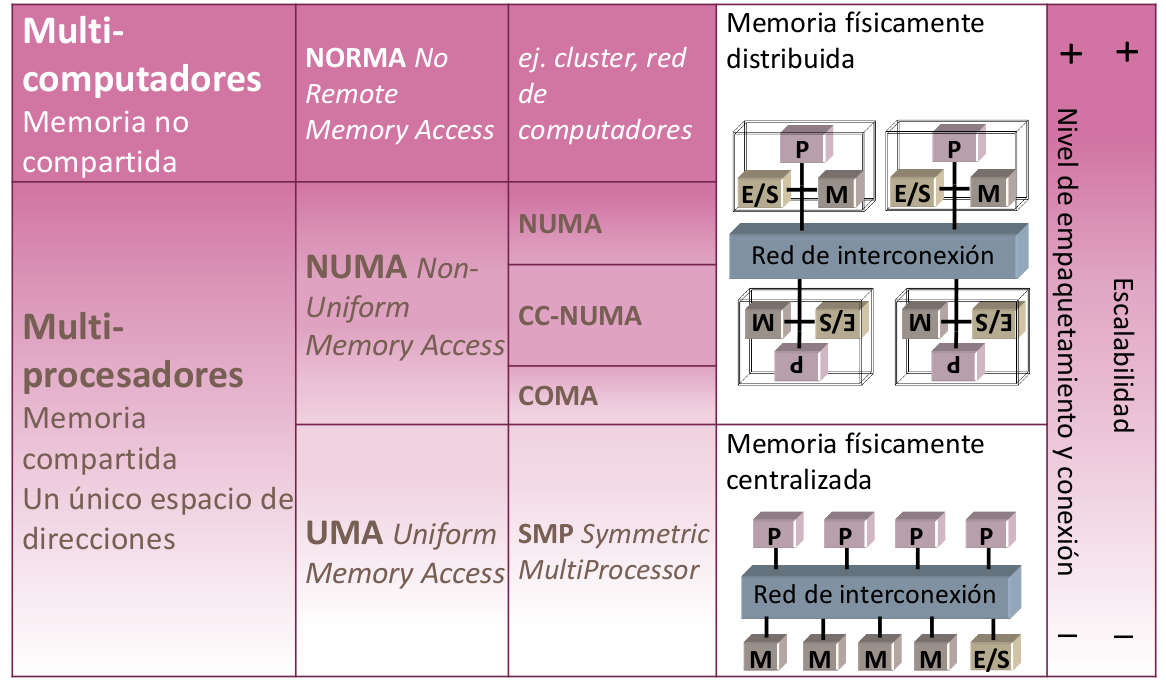
\includegraphics[width=1\textwidth]{20}
\caption{Clasificación de sistemas con múltiples procesadores}
\label{clasificacion_multip}
\end{figure}

A raíz de la aparición de multiprocesadores con memoria físicamente distribuida surgieron nuevas denominaciones para sistemas con múltiples procesadores. Los multiprocesadores se empezaron a clasificar entonces, en función de la uniformidad en el acceso a memoria, en dos grupos (\hyperref[clasificacion_multip]{Figura \ref*{clasificacion_multip}}):

\begin{enumerate}[\color{azul}{\bf $\heartsuit$}]
\item \textbf{\textcolor[rgb]{0.2,0.4,0.8}{Multiprocesadores con acceso a memoria uniforme}} o UMA (\textit{\textcolor[rgb]{0.2,0.4,0.8}{Uniform Memory Access}}): el tiempo de acceso de los procesadores a una determinada posición de memoria principal es igual sea cual sea el procesador. El acceso a una posición de memoria caché es igual para todos los procesadores.
\item \textbf{\textcolor[rgb]{0.2,0.4,0.8}{Multiprocesadores con acceso a memoria no uniforme}} o NUMA (\textit{\textcolor[rgb]{0.2,0.4,0.8}{Not-Uniform Memory Acess}}): el tiempo de acceso a una posición de memoria depende del procesador, ya que un procesador tardará menor tiempo en acceder al bloque de memoria local que al situado junto a otro procesador. Para que un NUMA sea escalable debe disminuirse la latencia media reduciendo el número de accesos de un procesador a posiciones de memoria situadas en bloques de memoria localizados en nodos remotos. Para ello necesitan distribuirse los códigos y datos de forma que en la memoria de un procesador estén los datos y código que utiliza. Si tenemos un hardware que evite incoherencias, podemos trasladar a la caché líneas de memoria y así aprovechar mejor el ancho de banda. Hay tres subgrupos:
\begin{enumerate}[$\longrightarrow$]
\item \textbf{\textcolor[rgb]{0.2,0.4,0.8}{NCC-NUMA}} (\textit{\textcolor[rgb]{0.2,0.4,0.8}{Non-Cache Non-Uniform Memory Access}}): no incorporan hardware para evitar problemas por incoherencias entre cachés de distintos nodos. Esto hace que los datos modificables compartidos no se puedan trasladar a caché de nodos remotos, se debe acceder a ellos individualmente a través de la red. Para el programador es el más difícil de programar pues debe mantener la coherencia entre cachés él mismo a nivel software. 
\item \textbf{\textcolor[rgb]{0.2,0.4,0.8}{CC-NUMA}} (\textit{\textcolor[rgb]{0.2,0.4,0.8}{Cache-Coherent Non-Uniform Memory Access}}): tienen hardware para mantener coherencia entre cachés de distintos nodos. El hardware añadido para mantenimiento de coherencia supone un coste añadido e introduce un retardo que hace que estos sistemas escalen en menor grado que un NUMA.
\item \textbf{\textcolor[rgb]{0.2,0.4,0.8}{COMA}} (\textit{\textcolor[rgb]{0.2,0.4,0.8}{Cache Only Memory Access}}): En estas arquitecturas la memoria local de los procesadores se gestiona como caché. El sistema de mantenimiento de coherencia se encarga de llevar dinámicamente el código y los datos a los nodos donde se necesiten. Permite \textit{\textcolor[rgb]{0.2,0.4,0.8}{replicación}}\footnote{Se prefiere cuando el bloque se usa en varios nodos} y \textit{\textcolor[rgb]{0.2,0.4,0.8}{migración}}\footnote{Se prefiere cuando un bloque se usa en mayor medida por otro nodo diferente al nodo donde se encuentra} de bloques de memoria en función de su frecuencia de uso en los nodos. Tienen mayor retardo hardware que los CC-NUMA. No existe actualmente ningún sistema comercial COMA.
\end{enumerate}
\end{enumerate}

\textcolor[rgb]{0.2,0.4,0.8}{\subsection{Nota histórica}}
El paralelismo a nivel de datos surgió en los procesadores en los años 90.

El paralelismo a nivel de instrucción surgió en los procesadores en los años 80, aunque el primer prototipo es de los 60.

El paralelismo a nivel de thread explícito con una instancia del SO tuvo sus primer prototipo en 1975 y explícito con múltiples instancias del SO (multicomputadores), en 1985.

El objetivo de esta parte es ver cuando ha ido surgiendo cada cosa y tambien ver que a partir de los 2000 no ha surgido casi nada nuevo sino que se ha mejorado segun ha ido avanzando la tecnologia que ha ido surgiendo lo que ya habia.

\textcolor[rgb]{0.2,0.4,0.8}{\section{Evaluación de prestaciones de una arquitectura}}
\textcolor[rgb]{0.2,0.4,0.8}{\subsection{Medidas usuales para evaluar prestaciones}}
Para evaluar un sistema de computador necesitaremos ejecutar un programa que tenga unas entradas y devuelva unas salidas. Podemos evaluar distintas partes de un sistema computador como el procesador, el sistema de memoria, el sistema de comunicación entre distintos computadores (en este caso las entradas serían los mensajes a transferir). En resumen, para evaluar cualquier sistema, se utilizan siempre las mismas medidas: tiempo de respuesta (tiempo desde que se introducen las entradas al sistema hasta que se obtienen los resultados) y productividad (número de entradas procesadas por unidad de tiempo).

\textcolor[rgb]{0.2,0.4,0.8}{\subsubsection{Tiempo de respuesta de un programa en una arquitectura}}
Si usamos el comando \verb*|time| en linux antes de ejecutar un programa obtenemos tres números: elapsed, user y time.
\begin{enumerate}[\color{azul}{\bf $\heartsuit$}]
  \item \verb*|user|: se corresponde con el \textbf{\textcolor[rgb]{0.2,0.4,0.8}{tiempo de CPU de usuario}}, es decir, el tiempo de ejecución en el espacio de usuario.
  \item \verb*|sys|: se corresponde con el \textbf{\textcolor[rgb]{0.2,0.4,0.8}{tiempo de CPU de sistema}}, es decir, el tiempo en el nivel del kernel del sistema operativo.
  \item Y el tiempo asociado a las esperas devidas a I/O o asociados a la ejecución de otros programas.
\end{enumerate}


\begin{minted}{bash}
  $ time ./program.exe
  elapsed 5.4
  user 3.2
  sys 1.0
\end{minted}


\begin{enumerate}[\color{azul}{\bf $\heartsuit$}]
  \item \textcolor[rgb]{0.2,0.4,0.8}{\textbf{Real} (\textit{wall-clock time, elapsed time, real time})}: tiempo que tarda en ejecutar todo el programa.
  \item \textbf{\textcolor[rgb]{0.2,0.4,0.8}{$CPU$ $time=user+sys$}}: tiempo que tardan en ejecutar el código correspondiente a llamadas al sistema y el código correspondiente al código del programa. El tiempo de ejecución real/elapsed también incluye esperas de E/S, que no forman parte del CPU time. Por eso el tiempo real es mayor o igual al de CPU.
\end{enumerate}


Ahora bien, cuando tenemos una o varias hebras ejecutándose en el programa varían los resultados devueltos por \verb*|time|: 
\begin{enumerate}[\color{azul}{\bf $\heartsuit$}]
  \item \textbf{\textcolor[rgb]{0.2,0.4,0.8}{Con un flujo de control}}: 
  el tiempo que nos devuelve \textit{\textcolor[rgb]{0.2,0.4,0.8}{elapsed}} es mayor o igual al \textit{\textcolor[rgb]{0.2,0.4,0.8}{CPU time}}: $elapsed \geq CPU$ $time$
  \item \textbf{\textcolor[rgb]{0.2,0.4,0.8}{Con múltiples flujos de control}}: esta vez tenemos que:
  \begin{enumerate}[$\longrightarrow$]
   \item $elapsed < CPU$ $time$
   \item $elapsed \geq \frac{CPU~time}{numero~flujos~control}$
  \end{enumerate}
  Ya que el elapsed será el thread que más tiempo tarde en ejecutarse y el CPU time será la suma de los tiempos de cpu de ambos thread.
\end{enumerate}


En el ejemplo anterior, $3.2+1.0$ es el $78\%$ del tiempo transcurrido (que en total ha sido $5.4$).

Algunas alternativas para obtener tiempos de ejecución son:

\begin{center}
\begin{tabular}{|c|c|c|c|}
\hline
\rowcolor[rgb]{0.2,0.4,0.8} \textcolor[rgb]{1,1,1}{Función} & \textcolor[rgb]{1,1,1}{Fuente} & \textcolor[rgb]{1,1,1}{Tipo} & \textcolor[rgb]{1,1,1}{Resolución aprox ($\mu s$)} \\
\hline
\verb*|time| & SO(/usr/bin/time) & elapsed, user, system & 10000 \\
\hline
\verb*|clock()| & SO (time.h) & CPU & 10000 \\
\hline
\verb*|gettimeofday()| & SO (sys/time.h) & elapsed & 1 \\
\hline
\verb*|clock_gettime()| / \verb*|clock_getres()| & SO (time.h) & elapsed & 0.001 \\
\hline
\verb*|omp_get_wtime()| / \verb*|omp_get_wtick()| & OpenMP (omp.h) & elapsed & 0.001 \\
\hline
\verb*|SYSTEM_CLOCK()| & Fortran & elapsed & 1 \\
\hline
\end{tabular}
\end{center}

\verb*|clock()| no obtiene el tiempo real. \verb*|clock_gettime()| y las funciones de OMP tienen muy buena precisión a la hora de calcular tiempo, a nivel de nanosegundos. Esta precisión depende de la plataforma. 

Cuando el programa sea secuencial usaremos \verb*|clock_gettime()| y cuando sea paralelo, las de OMP.

\textcolor[rgb]{0.2,0.4,0.8}{\subsubsection{Tiempo de CPU}}
% Para ilustrar el proceso de evolución experimentado y las perspectivas futuras se utiliza una expresión que relaciona el tiempo de CPU de un programa con tres características, a partir de las cuales se pueden extraer consecuencias relacionadas con la influencia de la tecnología, el compilador y la arquitectura en las prestaciones:

Podemos calcular el tiempo de CPU que tendrá nuestro programa nosotros mismos, ya que el tiempo de CPU depende de número de instrucciones del programa y el tiempo medio por instrucción. El número de instrucciones es fácil de obtener y el tiempo medio por instrucción, se puede obtener como el número medio de ciclos por instrucción por el tiempo de cada ciclo, y éstos datos se pueden calcular dinámicamente.

\begin{equation}
\label{eq:primera}
T_{tarea} = NI \cdot t_{medio\_por\_instr} = NI \cdot (CPI \cdot T_{ciclo}) = NI \cdot (\frac{CPI}{f})
\end{equation}

donde $T_{tarea}$ es el tiempo de CPU de un programa (también se denota como $T_{CPU}$), $NI$ es el número de instrucciones máquina del programa, $CPI$  es el número medio de ciclos por instrucción y $T_{ciclo}$, el periodo de reloj del procesador (inverso de la frecuencia del procesador, $f$). El valor de $CPI$ se puede expresar como:

\begin{equation}
\label{eq:segunda}
CPI = \frac{Ciclos~de~reloj~programa}{NI} = \frac{\sum_{i=1}^n NI_i \cdot CPI_i}{NI}
\end{equation}

donde $CPI_i$ es el número medio de ciclos de las instrucciones de tipo $i$ (uno de los $n$ tipos de instrucciones, ya que $i=1,\cdots,n$), y $NI_i$ es el número de instrucciones de ese tipo.

De esto, deducimos por tanto que el tiempo de CPU de un programa es:

\begin{equation}
\label{eq:tercera}
T_{CPU} = Ciclos~del~programa \cdot T_{ciclo} = \frac{Ciclos~del~programa}{Frecuencia~de~reloj}
\end{equation}

\begin{enumerate}[\color{azul}{\bf $\heartsuit$}]
  \item $NI$ depende del \textit{\textcolor[rgb]{0.2,0.4,0.8}{repertorio de instrucciones}} y del \textit{\textcolor[rgb]{0.2,0.4,0.8}{compilador}}
  \item $CPI$ viene determinado por el \textit{\textcolor[rgb]{0.2,0.4,0.8}{repertorio de instrucciones}} y la \textit{\textcolor[rgb]{0.2,0.4,0.8}{organización del computador}}
  \item $T_{ciclo}$ depende de las prestaciones que proporcione la \textit{\textcolor[rgb]{0.2,0.4,0.8}{tecnología}} y de la \textit{\textcolor[rgb]{0.2,0.4,0.8}{organización del computador}}.
\end{enumerate}

El valor de CPI se puede mejorar con procesadores superescalares ejecutando varias instrucciones en paralelo.

Al afectar la organización del computador tanto a $CPI$ como a $f$, la métrica importante es el cociente $\frac{CPI}{f}$: aunque se utilicen frecuencias mayores, si se produce un incremento del mismo orden en CPI, las prestaciones no aumentarían.

La expresión (\ref{eq:primera}) para $T_{tarea}$ se puede utilizar para reflejar características de los procesadores en relación con el aprovechamiento del paralelismo entre instrucciones:

\begin{equation}
\label{eq:cuarta}
T_{CPU} = NI \cdot \underbrace{(\frac{CPE}{IPE})}_{CPI} \cdot T_{ciclo}
\end{equation}

donde $CPE$ es el número medio de ciclos entre inicios de ejecución de instrucciones, es decir, ciclos entre \textit{\textcolor[rgb]{0.2,0.4,0.8}{emisión de instrucciones}} a ejecutar (\textit{\textcolor[rgb]{0.2,0.4,0.8}{Ciclos Por Emisión}}); e $IPE$, el número medio de instrucciones que se emiten (\textit{\textcolor[rgb]{0.2,0.4,0.8}{Instrucciones Por Emisión}}). El cociente entre ambos no es más que otra forma de contar el número de ciclos por instrucción. 

\begin{figure}
\centering
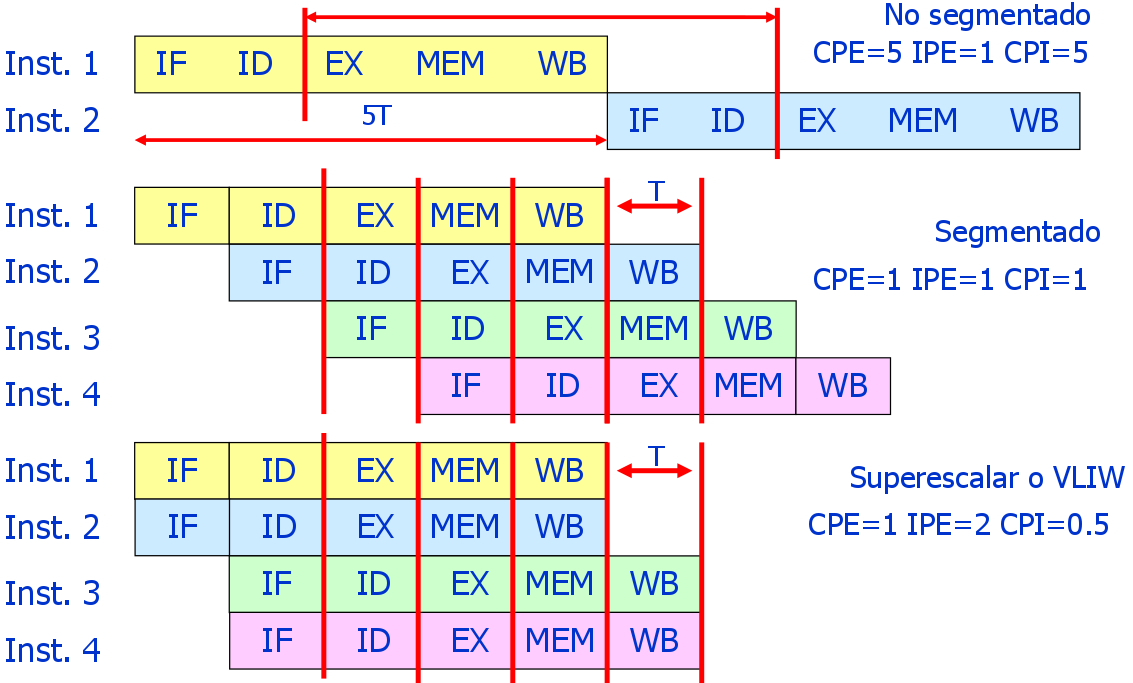
\includegraphics[width=1\textwidth]{23}
\caption{Ejemplos de valores característicos de CPE, IPE y CPI según las arquitecturas segmentadas, superescalares y VLIW}
\label{ejemplos_cpe}
\end{figure}

Así, como se muestra en la \hyperref[ejemplos_cpe]{Figura \ref*{ejemplos_cpe}}, en el caso de:
\begin{enumerate}[\color{azul}{\bf $\heartsuit$}]
\label{segmentado_tipos}
  \item \textit{\textcolor[rgb]{0.2,0.4,0.8}{Un procesador no segmentado}} en el que todas las instrucciones tienen igual duración (por ej: $CPI = 5$), el número de ciclos entre etapas de emisión es igual a $CPE = CPI$ (en este caso $CPE = 5$). Como cada vez se emite sólo una instrucción, $IPE = 1$. Tardaríamos un tiempo 5T en ejecutar una instrucción.
  \item \textit{\textcolor[rgb]{0.2,0.4,0.8}{Un procesador segmentado}} a pleno rendimiento se emitiría una instrucción por ciclo en cada ciclo`de reloj, por lo que $CPE = 1$ e $IPE = 1$, teniéndose que $CPI = 1$ (en cada ciclo se termina de ejecutar una instrucción). El tiempo de ejecución sería igual al tiempo de ejecución de una instrucción entre el número de etapas en las que se ha segmentado. 
  \item En \textit{\textcolor[rgb]{0.2,0.4,0.8}{los procesadores superescalares}} se podría emitir más de una instrucción por ciclo en cada ciclo. En el ejemplo de la \hyperref[ejemplos_cpe]{Figura \ref*{ejemplos_cpe}} se emiten dos instrucciones por ciclo, por lo que $CPE = 1$ e $IPE = 2$, por lo que $CPI = 0.5$. % Aumenta la productividad.
\end{enumerate}

También podemos recoger en la ecuación (\ref{eq:primera}) las características del repertorio de instrucciones según las posibilidades de codificación que presenta, el número de instrucciones, $NI$, se puede expresar en términos del número de operaciones que realiza el programa, $Noper$, y del número medio de operaciones que puede codificar una instrucción, $Op\_instr$:

\begin{equation}
\label{eq:quinta}
  T_{CPU}=(\frac{Noper}{Op\_instr}) \cdot CPI \cdot T_{ciclo}
\end{equation}

Así, si consideramos el ejemplo de procesamiento SIMD del \hyperref[procesador_vectorial]{procesador vectorial} y el \hyperref[procesador_matricial]{procesador matricial}, el número de instrucciones que se ejecutan es $Noper = 12$. Como existen cuatro elementos de procesamiento que trabajan simultáneamente, cada instrucción codifica cuatro operaciones, $Op\_instr=4$, y el programa a ejecutar consta de tres instrucciones del repertorio del procesador matricial ($NI = 3$).

\textcolor[rgb]{0.2,0.4,0.8}{\subsubsection{Productividad: MIPS y MFLOPS}}
Los \textbf{\textcolor[rgb]{0.2,0.4,0.8}{MIPS}} (\textit{\textcolor[rgb]{0.2,0.4,0.8}{Millones de Instrucciones por Segundo}}) y los \textbf{\textcolor[rgb]{0.2,0.4,0.8}{MFLOPS}} (\textit{\textcolor[rgb]{0.2,0.4,0.8}{Millones de Operaciones en Coma Flotante por Segundo}}) son medidas que pretenden caracterizar el nivel de prestaciones de un computador y facilitar la comparación entre distintos sistemas a través de una única cantidad.

La definición de los MIPS en términos de $T_{CPU}$ se proporciona en la siguiente expresión:

\begin{equation}
  \label{eq:sexta}
  MIPS = \frac{NI}{T_{CPU} \cdot 10^6} = \frac{f}{CPI \cdot 10^6}
\end{equation}

Esta medida puede variar según el programa, por lo que no sirve como medida característica de una máquina. Además, \textit{\textcolor[rgb]{0.2,0.4,0.8}{depende del repertorio de instrucciones}}, por lo que tampoco permite comparar máquinas con repertorios distintos y, puede ser inversamente proporcional a las prestaciones (valores mayores de MIPS corresponden a peores prestaciones), ya que los MIPS miden la velocidad de ejecución de las instrucciones. Por ejemplo, si dos programas tardan lo mismo pero uno utiliza más instrucciones que el otro (porque uno utiliza repertorio CISC y el otro, el repertorio RISC) el que utiliza más instrucciones tendrá más MIPS y erróneamente diremos que proporciona más prestaciones.

Los MFLOPS plantean una problemática similar a los MIPS y su fórmula es:

\begin{equation}
  \label{eq:septima}
  MFLOPS = \frac{Operaciones~en~coma~flotante}{T_{CPU} \cdot 10^6}
\end{equation}

No es una medida adecuada para todos los programas ya que sólo tiene en cuenta las operaciones en coma flotante. Además, ni el conjunto de instrucciones en coma flotante es el mismo para todas las máquinas ni tampoco el coste de dichas instrucciones (la precisión puede ser diferente, pueden no consumir el mismo número de ciclos, etc).

Para paliar este último problema, se utilizan los \textbf{\textcolor[rgb]{0.2,0.4,0.8}{MFLOPS normalizados}}, que se obtienen dando un peso relativo a cada instrucción para poner de manifiesto su mayor coste con respecto a la instrucción en coma flotante con menor coste.

\textcolor[rgb]{0.2,0.4,0.8}{\subsection{Conjunto de programas de prueba (Benchmark)}}
% Para evaluar una arquitectura, hay que considerar tanto las medidas de prestaciones que caracterizan a la arquitectura como las medidas de prestaciones que permiten comparar arquitecturas con igual uso en el nivel de abstracción superior.

% Es difícil encontrar un único programa que ponga de relieve todas estas propiedes del elemento del computador a evaluar, pero, en general, se desea que éste programa tenga las siguientes propiedades:
Las medidas de prestaciones que realicemos o que nos ofrezcan terceros deben cumplir las siguientes propiedades:
\begin{enumerate}[\color{azul}{\bf $\heartsuit$}]
  \item \textbf{\textcolor[rgb]{0.2,0.4,0.8}{Fiabilidad}}: las medidas deben obtenerse procesando un conjunto de entradas que sea representativo del que se pueden esperar en el funcionamiento habitual del sistema. También, para que sean fiables, los valores de las medidas deberían ser reproducibles. 
  \item \textbf{\textcolor[rgb]{0.2,0.4,0.8}{Permitir comparar diferentes realizaciones de un sistema o diferentes sistemas}}: para que se puedan comparar diferentes realizaciones de un sistema o diferentes sistemas, sobre la base de medidas de tiempo de respuesta y productividad, éstas se deben tomar con las mismas secuencias de entradas en las diferentes implementaciones. Por lo que se necesitan entradas por los interesados, tanto fabricantes e investigadores como vendedores o usuarios.
\end{enumerate}

\textcolor[rgb]{0.2,0.4,0.8}{\subsubsection{Tipos de Benchmarks}}
\begin{enumerate}[\color{azul}{\bf $\heartsuit$}]
  \item \textcolor[rgb]{0.2,0.4,0.8}{\textbf{De bajo nivel o microbenchmark}}: evalúan las prestaciones de distintos aspectos de la arquitectura o del software: el procesador, la memoria, etc. Un ejemplo de microbenchmark para redes de interconexión es el test ping-pong.
  \item \textcolor[rgb]{0.2,0.4,0.8}{\textbf{Kernels}}: son trozos de código muy utilizados en diferentes aplicaciones. Por ejemplo: multiplicación de matrices, resolución de sistemas de ecuaciones, producto escalar... Junto con los microbenchmark, son útiles para encontrar los puntos fuertes de cada máquina y así poder explicar las diferencias en prestaciones entre diferentes máquinas.
  \item \textcolor[rgb]{0.2,0.4,0.8}{\textbf{Programas sintéticos}}: Son también trozos de código, pero no pretenden obtener un resultado con significado. Es la peor opción, ya que no se utilizan en aplicaciones reales. Ejemplos: Dhrystone ó Whetstone.
  \item \textcolor[rgb]{0.2,0.4,0.8}{\textbf{Programas reales}}: Son programas disponibles comercialmente o gratuitos utilizados en el sector de computadores que pretenden evaluar, como por ejemplo, bases de datos, servidores web, etc.
  \item \textcolor[rgb]{0.2,0.4,0.8}{\textbf{Aplicaciones diseñadas}}: Se diseñan aplicaciones que pretenden representar a aquellas para las que se utiliza el computador. Resultan útiles cuando no existen para estas aplicaciones programas disponibles. Cuanto más se acerquen a \textit{\textcolor[rgb]{0.2,0.4,0.8}{aplicaciones reales}}, mayor será la fiabilidad que ofrecen.
\end{enumerate}

\textcolor[rgb]{0.2,0.4,0.8}{\subsubsection{Benchmark suites}}
Las \textcolor[rgb]{0.2,0.4,0.8}{\textit{benchmark suites}} son un conjunto de programas de prueba promovidos por ciertas instituciones en los que se suplen las limitaciones de los benchmark con la presencia de otros. Estos conjuntos cambian periódicamente adaptándose a los nuevos avances que van surgiendo, mejorar sus resultados, etc. Las benchmark suites más destacadas son:
\begin{description}
  \item[SPEC CPU2006]: se usa para la evaluación de operaciones con enteros (CINT2006) y con punto flotante (CFP2006) en un core. Es un benchmark del tipo aplicaciones reales:
  \begin{enumerate}[\color{azul}{\bf $\heartsuit$}]
    \item \textbf{\textcolor[rgb]{0.2,0.4,0.8}{CINT2006}}: compilador gcc, compresor bzip2, planificación de vehículos de transporte, inteligencia artificial, compresión de vídeo...
    \item \textbf{\textcolor[rgb]{0.2,0.4,0.8}{CFP2006}}: dinámica de fluidos, dinámica molecular, reconocimiento de voz...
  \end{enumerate}
  Las herramientas que usa son C, C++ y Fortran.
  \item[SPEC OMP 2001 (SPEC OpenMP)]: es un benchmark paralelo. Con este benchmark se evalúan prestaciones de aplicaciones para SMP programas con OpenMP. Permite evaluar el procesador, el sistema de memoria, el sistema operativo y el compilador. Está basado en el benchmark SPEC CPU2000. Ofrece ls códigos fuente para poder analizar las prestaciones del compilador con diferentes optimizaciones. Se usa en el ámbito científico y su estilo es de variables compartidas.
  \item[SPEC HPC2002]: está basado en aplicaciones de altas prestaciones y tiene como objetivo la evaluación de computadores de altas prestaciones. Permite evaluar: los procesadores, el sistema de interconexión, los compiladores, la implementación de OpenMP y MPI, y el sistema de E/S. Su área de aplicación es científica. Su estilo se basa en variables compartidas, paso de mensajes y combinación de ambos. 
  \item[TPC (Transaction Processing Performance Council)]: El grupo TPC ha desarrollado un conjunto de benchmark que evalúa diferentes aplicaciones comerciales de servidores:
  \begin{enumerate}[\color{azul}{\bf $\heartsuit$}]
    \item \textcolor[rgb]{0.2,0.4,0.8}{\textbf{TPC-C}} analiza procesamiento de transacciones OLTP.
    \item \textcolor[rgb]{0.2,0.4,0.8}{\textbf{TPC-H}} y \textcolor[rgb]{0.2,0.4,0.8}{\textbf{TPC-R}} evalúan cargas de trabajo de sistema de soporte de decisiones (DSS). TPC-H soporta modificaciones concurrentes de datos y peticiones improvisadas orientadas al comercio y a la insdustria. TPC-R permite optimizaciones adicionales basadas en el conocimiento de las peticiones.
    \item \textcolor[rgb]{0.2,0.4,0.8}{\textbf{TPC-W}} evalúa aplicaciones de comercio electrónico, genera transaciones orientadas al comercio.
    \item \textcolor[rgb]{0.2,0.4,0.8}{\textbf{TPC-App}} evalúa servidores web y de aplicaciones.
  \end{enumerate}
  Los benchmark TPC son entradas software comercial (bases de datos, servidores de información de Internet) y carga de trabajo diseñada.
  \item[NPB2, NPB3 (NAS Parallel Benchmark)]: son benchmark paralelos. Ambos constan de cinco núcleos y tres pseudo-aplicaciones diseñadas. NPB2 está implementado con MPI. NPB3 consta de implementaciones de OpenMP, Java y HPF. Se usa en el ámbito científico. Su estilo es paso de mensajes y variables compartidas.
  \item[Implementaciones de la bibloteca BLAS (Basic Linear Algebra Subprograms)]: evalúan cores con operaciones del álgebra lineal. Incluye operaciones con:
  \begin{enumerate}[\color{azul}{\bf $\heartsuit$}]
    \item vectores, como producto escalar o AXPY (\textit{\textcolor[rgb]{0.2,0.4,0.8}{\textbf{A}lpha \textbf{X P}lus \textbf{Y}}})
    \item vector-matriz, como producto matriz por vector
    \item matriz-matriz como producto de matrices (\textit{\textcolor[rgb]{0.2,0.4,0.8}{GEMM-GEneral Matrix Multiply}})
  \end{enumerate}
  Hay implementaciones con diferentes herramientas de programación y optimizadas para diferentes arquitecturas.
  \item[LINPACK]: se utiliza para clasificar a los computadores en la lista top500 .el núcleo de este programa es una rutina denominada DAXPY (\textit{\textcolor[rgb]{0.2,0.4,0.8}{\textbf{D}ouble precision-real \textbf{A}lpha \textbf{X P}lus \textbf{Y}}}) que multiplica un vector por una constante y los suma a otro vector. Las prestaciones obtenidas se escalan con el valor del tamaño del vector:
  \begin{minted}{c++}
  for (i=0; i<N; i++)
      y[i] = alpha*x[i] + y[i];
  \end{minted}
\end{description}

\textcolor[rgb]{0.2,0.4,0.8}{\subsection{Ganancia en prestaciones}}
\textcolor[rgb]{0.2,0.4,0.8}{\subsubsection{Ganancia en velocidad ó Speed-up}}
Si en un computador se incrementan las prestaciones de un recurso haciendo que su velocidad sea \textit{\textcolor[rgb]{0.2,0.4,0.8}{p veces mayor}} (por ejemplo: \textit{\textcolor[rgb]{0.2,0.4,0.8}{p procesadores}} en lugar de uno), el incremento de velocidad que se consigue en la nueva situación con respecto a la previa (\textit{\textcolor[rgb]{0.2,0.4,0.8}{máquina base}}) se expresa mediante la \textbf{\textcolor[rgb]{0.2,0.4,0.8}{ganancia de velocidad}} ó \textbf{\textcolor[rgb]{0.2,0.4,0.8}{\textit{speed-up}}}, $S_p$:

\begin{displaymath}
S_p = \frac{V_p}{V_1} = \frac{T_1}{T_p}
\end{displaymath}

Siendo:
\begin{enumerate}[\color{azul}{\bf $\heartsuit$}]
  \item $V_1$ la velocidad de la máquina base
  \item $V_p$ la velocidad de la máquina mejorada (un factor $p$ en uno de sus componentes)
  \item $T_1$ tiempo de ejecución en la máquina base
  \item $T_p$ tiempo de ejecución en la máquina mejorada
\end{enumerate}

\textcolor[rgb]{0.2,0.4,0.8}{\subsubsection{Ley de Amdahl}}

\begin{figure}[!h]
    \centering
    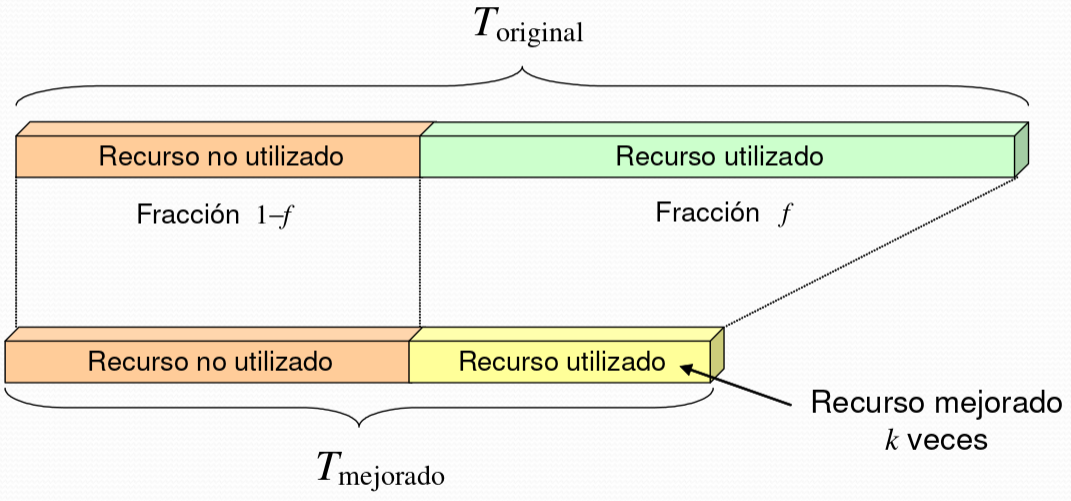
\includegraphics[width=0.7\textwidth]{113}
    \caption{Tiempo original vs tiempo mejorado}
    \label{tiempos}
\end{figure}

La mejora de la velocidad, $S$, que se puede obtener cuando se mejora un recurso de una máquina en un factor $p$ (o $k$ según la \hyperref[tiempos]{Figura \ref*{tiempos}}) está limitada por:

\begin{displaymath}
S \leq \frac{p}{1+f(p-1)}
\end{displaymath}

donde $f$ es la fracción del sistema que utiliza la mejora, y $p$ indica en cuanto se consigue mejorar esa fracción. 

Por ejemplo: si un programa pasa un $25\%$ de su tiempo de ejecución en una máquina realizando instrucciones de coma flotante, y se mejora la máquina haciendo que estas instrucciones se ejecuten en la mitad de tiempo, entonces $p=2$, $f=0.75$ y:

\begin{displaymath}
S \leq \frac{2}{1+0.75} = 1.14
\end{displaymath}

\begin{center}
\framebox[1.1\width]{Hay que mejorar el caso más frecuente (lo que más se usa)} \par
\end{center}

Para deducir esta ecuación debemos partir del \textit{\textcolor{azul}{speedup}} obtenido al cambiar el componente. 

El tiempo sin mejorar sería:

\begin{displaymath}
    T_{original} = f \cdot T_{original} + (1-f)\cdot T_{original}
\end{displaymath}

y el tiempo mejorado al aplicar el factor $p$ sería:

\begin{displaymath}
    T_{mejorado} = f \cdot T_{original} + \frac{(1-f) \cdot T_{original}}{p}
\end{displaymath}

Y el \textcolor{azul}{\textit{speedup}} obtenido sería:

\begin{displaymath}
    S = \frac{T_{original}}{T_{mejorado}} = \frac{T_{original}}{f \cdot T_{original} + \frac{(1-f)\cdot T_{original}}{p}} = \frac{T_{original}}{T_{original}} \cdot \Bigg(\frac{1}{f + \frac{1-f}{p}} \Bigg)  = \frac{1}{f + \frac{1-f}{p}} = \frac{p}{1 + f\cdot(p-1)}
\end{displaymath}

Otra forma de ver esta ley es la siguiente: tenemos un componente que, para un determinado programa, se utiliza una fracción $f$ de tiempo, ¿cómo mejora el tiempo de ejecución del programa al cambiar dicho componente por otro $p$ veces más rápido?

\begin{displaymath}
    T_{mejorado} = (1 - f) \cdot T_{original} + \frac{f \cdot T_{original}}{p}
\end{displaymath}

Para deducirla, hacemos el \textit{\textcolor{azul}{speedup}} como antes:

\begin{displaymath}
    S = \frac{T_{original}}{T_{mejorado}} = \frac{T_{original}}{(1-f)\cdot T_{original} + \frac{f \cdot T_{original}}{p}} = \frac{1}{1 - f + \frac{f}{p}}
\end{displaymath}

La mejora sólo se verá afectada por la fracción de tiempo que utiliza dicho recurso, lo demás no varía (\hyperref[tiempos]{Figura \ref*{tiempos}}). Por tanto, cuando $f=0$ no hay ninguna mejora y cuando $f=1$ el tiempo de ejecución mejora $k$ veces, igual que el componente.

% \begin{displaymath}
% T_1 = f \cdot T_1 + (1 - f)T_1
% \end{displaymath}
% \begin{displaymath}
% T_p \geq f \cdot T_1 + \frac{(1-f)T_1}{p}
% \end{displaymath}

% Y sustituir estos valores en la ecuación de la ganancia de velocidad:

% \begin{displaymath}
% S = \frac{T_1}{T_p} = \frac{f \cdot T_1 + (1 - f)T_1}{f \cdot T_1 + \frac{(1 - f)T_1}{p}} = 
% \end{displaymath}

% Sacamos factor común de $T_1$ y hacemos mínimo común múltiplo:

% \begin{displaymath}
% = \frac{T_1(f+1-f)}{T_1(f+\frac{1-f}{p})} = \frac{1}{f + \frac{1 - f}{p}} = \frac{1}{\frac{fp + 1 - f}{p}} = \frac{p}{fp + 1 - f} =
% \end{displaymath}

% Ahora dividimos todos los miembros entre $f$
% \begin{displaymath}
% \frac{\frac{p}{f}}{\frac{fp}{f}+\frac{1}{f}-{f}{f}} = \frac{\frac{p}{f}}{p+\frac{1}{f}-1} = \frac{\frac{p}{f}}{(p-1)+\frac{1}{f}} =
% \end{displaymath}

% Quitamos las $f$:

% \begin{displaymath}
% = \frac{\frac{p}{f}}{\frac{(p-1)f + 1}{f}} = \frac{p}{(p-1)f + 1}
% \end{displaymath}

En relación con la eficacia de los computadores paralelos, la ley de Amdahl dice que dado que en un programa hay código secuencial que no puede paralelizarse, los procesadores no se podrían utilizar eficazmente.

\textcolor[rgb]{0.2,0.4,0.8}{\section{Ejercicios}}
\textcolor[rgb]{0.2,0.4,0.8}{\subsection{Ejercicio 3}}
\textcolor[rgb]{0.2,0.4,0.8}{\subsubsection{Resumen de los datos del enunciado}}
\begin{tabular}{c||c|c||c|c}
$I_i$ & $CPI_i^1$ & $NI_i^1$ & $CPI_i^2$ & $NI_i^2$ \\
\hline
CMP & $3$ & $0.2NI^1$ & - & - \\
BR & $4$ & $0.2NI^1$ & - & - \\
CMP-BR & $-$ & $-$ & $4$ & $0.2NI^1$ \\
Resto & $3$ & $0.6NI^1$ & $3$ & $0.6NI^1$
\end{tabular}

\begin{displaymath}
T_c^1 = T_c^2 - 0.25 \cdot T_c^2 = 0.75 \cdot T_c^2
\end{displaymath}

El número de instrucciones de salto condicional en la alternativa 1 coincide con el número de instrucciones CMP+BR porque ejecutamos los mismos programas con ambas alternativas.

En el resto teníamos incluída las instrucciones CMP, como las hemos puesto aparte, en el resto tenemos $0.6NI^1$

\textcolor[rgb]{0.2,0.4,0.8}{\subsubsection{Comparativa entre las dos alternativas}}
\begin{displaymath}
T_{CPU}^1 = \underbrace{((3 \cdot 0.8NI^1)}_{Resto+CMP} + \underbrace{4 \cdot 0.2NI^1)}_{BR} \cdot T_c = 3.2 \cdot NI^1 \cdot T_c^1
\end{displaymath}


\begin{displaymath}
T_{CPU}^2 = (\underbrace{(3 \cdot 0.6NI^1)}_{Resto} + \underbrace{(4 \cdot 0.2NI^1)}_{CMP-BR}) \cdot T_c^2 = 2.6 \cdot NI^1 \cdot T_c^2 
\end{displaymath}

Cogiendo la fórmula que hemos sacado a partir de los datos del enunciado, sustituimos en el tiempo de ciclo de la alternativa 1:

\begin{displaymath}
T_{CPU}^1 = \underbrace{((3 \cdot 0.8NI^1)}_{Resto+CMP} + \underbrace{4 \cdot 0.2NI^1)}_{BR} \cdot T_c = 3.2 \cdot NI^1 \cdot T_c^1 = 3.2 \cdot NI^1 \cdot \underbrace{0.75 \cdot T_c^2}_{T_c^1} = 2.4 \cdot NI^1 \cdot T_c^2
\end{displaymath}

Y concluimos que la alternativa 2 no merece la pena, pues aunque tenemos menos instrucciones, el tiempo de ciclo es mayor.

\textcolor[rgb]{0.2,0.4,0.8}{\subsection{Ejercicio 4}}

Ahora tenemos este tiempo de ciclo para la alternativa dos:

\begin{displaymath}
T_c^2 = 1.1 \cdot T_c^1
\end{displaymath}

Si sustituimos en el tiempo de cpu de la alternativa dos obtenemos:

\begin{displaymath}
T_{CPU}^2 = (\underbrace{(3 \cdot 0.6NI^1)}_{Resto} + \underbrace{(4 \cdot 0.2NI^1)}_{CMP-BR}) \cdot T_c^2 = 2.6 \cdot NI^1 \cdot T_c^2 = 2.6 \cdot NI^1 \cdot 1.1 \cdot T_c^1 = 2.86 \cdot NI^1 \cdot T_c^1
\end{displaymath}

En este caso si merecería la pena.

EXTRA: calcular los MIPS de cada alternativa:

\begin{displaymath}
MIPS^1 = \frac{NI^1}{3.2\cdot NI^1 \cdot T_c^1 \cdot 10^6}
\end{displaymath}

\begin{displaymath}
MIPS^2 = \frac{NI^2}{2.86 \cdot NI^1 \cdot T_c^1 \cdot 10^6} = \frac{0.8NI^1}{2.86 \cdot NI^1 \cdot T_c^1 \cdot 10^6} = \frac{1}{3.575 \cdot T_c^1 \cdot 10^6}
\end{displaymath}


La alternativa mejor según los MIPS sería la uno, lo cual es erróneo porque como hemos visto, la mejor es la dos.

\textcolor[rgb]{0.2,0.4,0.8}{\chapter{Programación paralela}}
\setcounter{section}{3}
\textcolor[rgb]{0.2,0.4,0.8}{\section{Herramientas, estilos y estructuras en programación paralela}}
\textcolor[rgb]{0.2,0.4,0.8}{\subsection{Problemas que plantea la programación paralela al programador. Punto de partida}}
\textcolor[rgb]{0.2,0.4,0.8}{\subsubsection{Problemas que plantea la programación paralela}}
Con la programación paralela, nos surgen nuevos problemas que no teníamos en programación secuencial:
\begin{enumerate}[\color{azul}{\bf $\heartsuit$}]
    \item \textcolor[rgb]{0.2,0.4,0.8}{\textbf{División en unidades de cómputo independientes (tareas)}}: el programador debe dividir su código en unidades independientes unas de las otras, llamadas tareas.
    \item \textcolor[rgb]{0.2,0.4,0.8}{\textbf{Agrupación/asignación de tareas o carga de trabajo (código, datos) en procesos/threads}}: después, debe asignar dichas tareas a distintos threads para que se ejecuten en paralelo.
    \item \textcolor[rgb]{0.2,0.4,0.8}{\textbf{Asignación a procesadores/núcleos}}: para conseguir paralelismo real el programador debe asignar cada thread a un procesador/núcleo diferente porque si asigna todo el trabajo a un único thread no tendríamos programación paralela sino concurrente.
    \item \textcolor[rgb]{0.2,0.4,0.8}{\textbf{Sincronización y comunicación}}: dichas tareas seguramente compartan datos, por tanto, deben estar sincronizadas para que el resultado de la ejecución sea correcto.
\end{enumerate}

Estos nuevos problemas debe abordarlos la herramienta de programación (el compilador), el programador o ambos.

\textcolor[rgb]{0.2,0.4,0.8}{\subsubsection{Punto de partida}}
Cuando se plantea obtener una versión paralela de una aplicación, se puede utilizar como punto de partida:
\begin{enumerate}[\color{azul}{\bf $\heartsuit$}]
    \item Un \textbf{\textcolor[rgb]{0.2,0.4,0.8}{código secuencial}} que resuelva el problema y, sobre este código de alto nivel buscar la paralelización.  La versión paralela va a depender de la descripción del problema que se ha utilizado en la versión secuencial de partida. Podría ocurrir que el programa secuencial no adminta una paralelización inmediata. Una ventaja de esta opción es que facilita el reparto del trabajo equitativo entre procesadores. 
    \item Otra posibilidad, sería partir de la \textbf{\textcolor[rgb]{0.2,0.4,0.8}{definición de la aplicación}}. Habría que buscar una descripción para el problema que admita paralelización, incluso se podrían exportar varias descripciones alternativas.
\end{enumerate}

Para facilitar el trabajo podemos apoyarnos en programas paralelos que aprovechen las características de la arquitectura y en bibliotecas de funciones paralelas. Hay diversas bibliotecas paralelas que porporcionan funciones que se utilizan en aplicaciones que requieren altas prestaciones como:
\begin{enumerate}[\color{azul}{\bf $\heartsuit$}]
    \item Un programa paralelo que resuelva un problema parecido.
    \item Versiones paralelas u optimizadas de bibliotecas de funciones como pueden ser BLAS (\textit{\textcolor[rgb]{0.2,0.4,0.8}{Basic Linear Algebra Subroutine}} o LAPACK (\textcolor[rgb]{0.2,0.4,0.8}{\textit{Linear Algebra PACKage}}))
\end{enumerate}

\textcolor[rgb]{0.2,0.4,0.8}{\subsection{Modos de programación}}
\textcolor[rgb]{0.2,0.4,0.8}{\subsubsection{SPMD (Single-Program Multiple Data)}}
En el modo \textbf{\textcolor[rgb]{0.2,0.4,0.8}{SPMD}} (\textit{\textcolor[rgb]{0.2,0.4,0.8}{Single Program Multiple Data}}), todos los códigos que se ejecutan en paralelo se obtienen compilando el mismo programa. Cada copia trabaja con un conjunto de datos distintos, y se ejecuta en un procesador diferente (\hyperref[prog_spmd]{Figura \ref*{prog_spmd}}).

En la práctica, tanto en multiprocesadores como en multicomputadores, se aplica en mayor medida el modo SPMD.

\begin{figure}[!h]
\centering
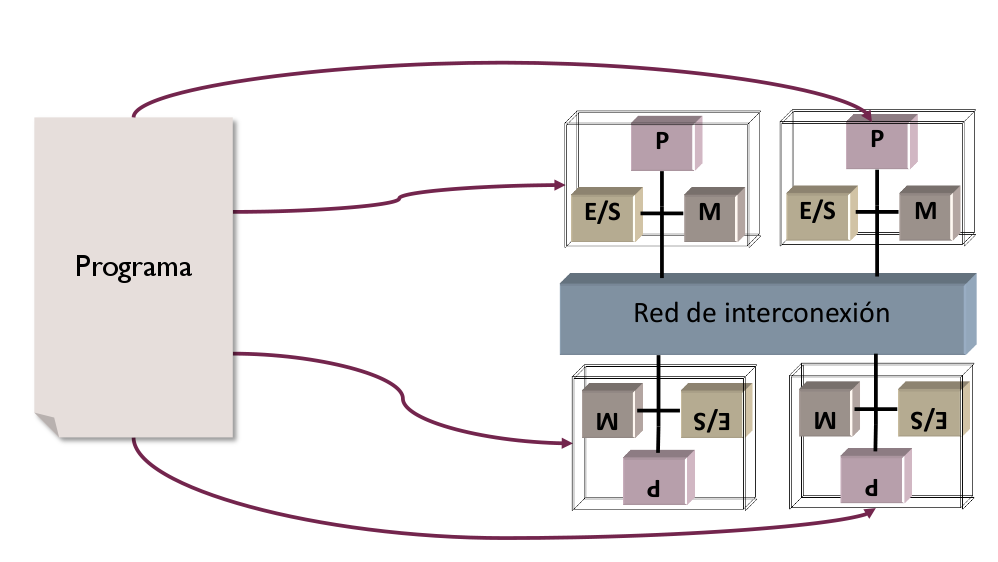
\includegraphics[width=0.5\textwidth]{24}
\caption{Programación SPMD}
\label{prog_spmd}
\end{figure}


\textcolor[rgb]{0.2,0.4,0.8}{\subsubsection{MPMD (Multiple Programs Multiple Data)}}
En el modo \textcolor[rgb]{0.2,0.4,0.8}{\textbf{MPMD}} (\textcolor[rgb]{0.2,0.4,0.8}{\textit{Multiple Programs Multiple Data}}), los códigos que se ejecutan en paralelo se obtienen compilando programas independientes. En este caso la aplicación a ejecutar se divide en unidades independientes. Cada unidad trabaja con un conjunto de datos y se asigna a un procesador distinto (\hyperref[prog_mpmd]{Figura \ref*{prog_mpmd}}).

\begin{figure}[!h]
\centering
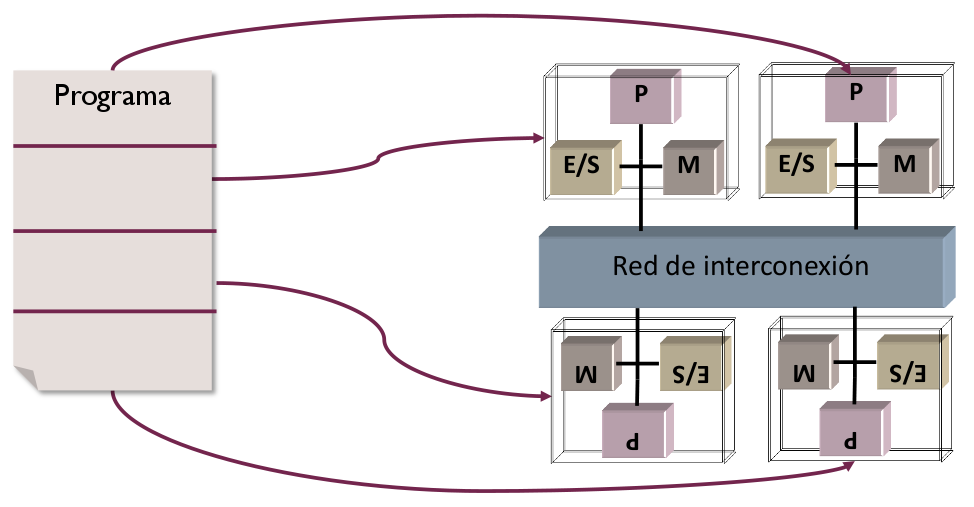
\includegraphics[width=0.5\textwidth]{25}
\caption{Programación MPMD}
\label{prog_mpmd}
\end{figure}

\newpage
\textcolor[rgb]{0.2,0.4,0.8}{\subsection{Herramientas para obtener código paralelo}}
Las herramientas para obtener programas paralelos deberían permitir de \textbf{\textcolor[rgb]{0.2,0.4,0.8}{forma explícita}} (el trabajo lo haría el \textcolor[rgb]{0.2,0.4,0.8}{\textit{programador}}) o \textcolor[rgb]{0.2,0.4,0.8}{\textbf{ímplicita}} (el trabajo lo haría la \textit{\textcolor[rgb]{0.2,0.4,0.8}{propia herramienta}}) la realización de las siguientes tareas:
\begin{enumerate}[\color{azul}{\bf $\heartsuit$}]
    \item Localizar paralelismo
    \item Distribuir la carga de trabajo entre procesos
    \item Crear y terminar procesos
    \item Comunicación y sincronización entre procesos
\end{enumerate}

La asignación de la carga de trabajo a procesadores puede quedar implícita en la asignación de ésta a procesos (la elección se deja al sistema operativo).

Hay varias alternativas para obtener un programa paralelo, la que requiere una mayor implicación del programador está en el nivel de abstracción más bajo (\hyperref[herramientas_paralelas]{Figura \ref*{herramientas_paralelas}}).

\begin{figure}[!h]
\centering
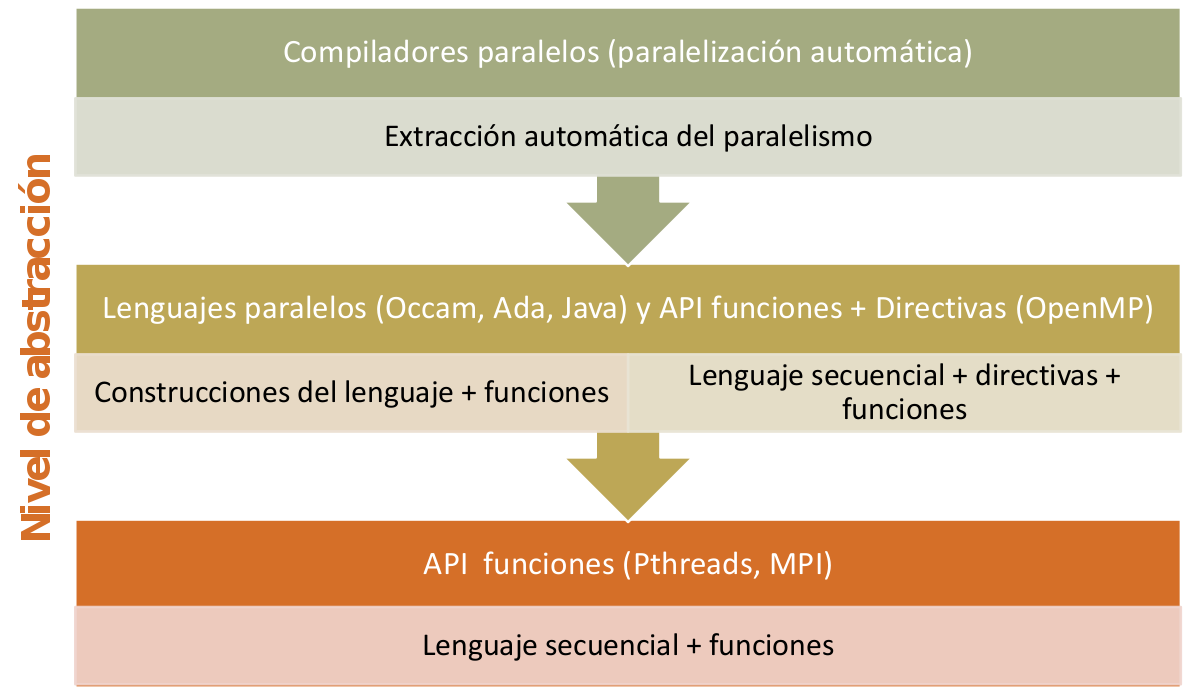
\includegraphics[width=0.5\textwidth]{26}
\caption{Herramientas de programación paralela clasificadas por su nivel de abstracción}
\label{herramientas_paralelas}
\end{figure}

\textcolor[rgb]{0.2,0.4,0.8}{\subsubsection{Bibliotecas de funciones para programación paralela}}
El programador utiliza un lenguaje secuencial y una biblioteca de funciones. El cuerpo de los procesos y hebras se escribe con lenguaje secuencial. El programador explícitamente se encaga de: 
\begin{enumerate}[\color{azul}{\bf $\heartsuit$}]
    \item Distribuir las tareas entre los procesos usando el lenguaje secuencial
    \item Crear o gestionar procesos e implementar la comunicación y sincronización, utilizando funciones de la biblioteca
    \item Puede elegir la distribución de los procesos entre procesadores
\end{enumerate}

Las ventajas de esta alternativa son:
\begin{enumerate}[\color{azul}{\bf $\heartsuit$}]
    \item Los programadores están familiarizados con los lenguajes secuenciales
    \item Las biliotecas están disponibles para todos los sistemas paralelos
    \item Las bibliotecas están más cercanas al hardware y dan al programador un control a más bajo nivel
    \item Se pueden utilizar a la vez bibliotecas para programar hebras y bibliotecas para programar procesos.
\end{enumerate}

Por ejemplo: PThread y MPI. Esta última incluye directivas, el uso de éstas sitúa al programador en un nivel de abstracción superior.

Un ejemplo para calcular el número pi usando MPI sería:
\begin{minted}[linenos]{c}
#include <mpi.h>
int main (int argc, char **argv) {
    double ancho, x, sum, lsum; int intervalos, i, nproc, iproc;

    if (MPI_Init(&argc, &argv) != MPI_SUCCESS) exit(1);     // Enrolar
    MPI_Comm_size(MPI_COMM_WORLD,&nproc);
    MPI_Comm_rank(MPI_COMM_WORLD,&iproc);
    intervalos = atoi(argv[1]);
    ancho=1.0/(double) intervalos; lsum= 0;

    // Localizar y asignar
    for (i = iproc; i<intervalos; i+=nproc) {
        x = (i+0.5)*ancho; lsum+=4.0/(1.0+x*x);
    }

    lsum*=ancho;

    // Comunicar/sincronizar
    MPI_Reduce(&lsum, &sum, 1, MPI_DOUBLE, MPI_SUM, 0, MPI_COMM_WORLD);

    // Desenrolar
    MPI_Finalize();
}    
\end{minted}

\textcolor[rgb]{0.2,0.4,0.8}{\subsubsection{Lenguajes paralelos y directivas del compilador}}
El uso de lenguajes paralelos o lenguajes secuenciales con directivas sitúan al programador en un nivel de abstracción superior, facilitando un poco el trabajo, aunque puede que sólo aprovechen un tipo de paralelismo: paralelismo de tareas o de datos. 

Los lenguajes paralelos ahorran estas tareas utilizando:
\begin{enumerate}[\color{azul}{\bf $\heartsuit$}]
    \item Construcciones propias del lenguaje, que además de distribuir la carga de trabajo pueden crear y terminar procesos.
    \item Directivas del compilador.
    \item Funciones de biblioteca que implementan en paralelo algunas operaciones usuales.
\end{enumerate}

Estos programas son más cortos y fáciles de entender que los programas secuenciales con bibliotecas para programación paralela.

Por ejemplo, para cálcular el número pi con directivas de OpenMP en C:
\begin{minted}[linenos]{c}
#include <omp.h>
#define NUM_THREADS 4
int main (int argc, char **argv) {
    double ancho, x, sum=0; int intervalos, i;
    intervalos = atoi(argv[1]);
    ancho=1.0/(double) intervalos;
    omp_set_num_threads(NUM_THREADS);

    // Crear y terminar
    #pragma omp parallel
    {
        // Localizar 
        #pragma omp for reduction (+:sum) /* Comunicar y sincronizar*/ private(x) \
                        schedule (dynamic) /* Agrupar y asignar*/
            for (i=0;i<intervalos;i++) {
                x = (i+0.5)*ancho; sum = sum + 4.0/(1.0+x*x);
            }
    }
    sum*=ancho;
    return 0;
}
\end{minted}

\textcolor[rgb]{0.2,0.4,0.8}{\subsubsection{Compiladores paralelos}}
El compilador extrae automáticamente paralelismo a nivel de bucle (paralelismo de datos) y de función (paralelismo de tareas) a partir de una versión secuencial del código. Para ello realizan análisis de dependencias entre bloques de código, con las dependencias de datos que vimos en el \hyperref[dependencias_datos]{tema anterior}.

Los compiladores paralelos aún están limitados a aplicaciones que exhiben un paralelismo regular, como cálculos a nivel de bucle. 

\textcolor[rgb]{0.2,0.4,0.8}{\subsection{Comunicaciones Colectivas}}
Las herramientas de programación paralela ofrecen comunicación entre procesos de distintos tipos para comunicar a los procesos que colaboran entre sí en la ejecución de un código.

\begin{figure}[!h]
\centering
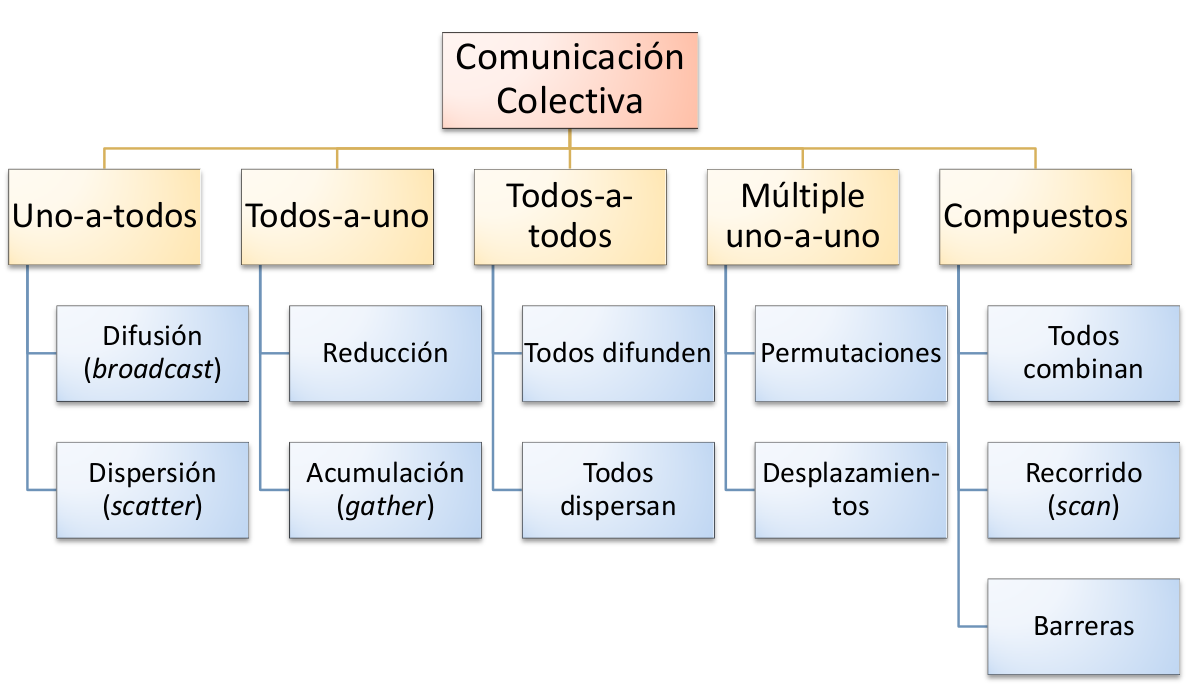
\includegraphics[width=1\textwidth]{27}
\caption{Comunicación paralela}
\label{comunicacion_paralela_esquema}
\end{figure}

La clasificación de las funciones colectivas (\hyperref[comunicacion_paralela_esquema]{Figura \ref*{comunicacion_paralela_esquema}}) se presenta en cinco grupos:
\begin{enumerate}[\color{azul}{\bf $\heartsuit$}]
    \item \textcolor[rgb]{0.2,0.4,0.8}{\textbf{Comunicación uno-a-todos}}: \label{uno_a_todos} Un proceso envía y todos los procesos reciben (\hyperref[comunicacion_uno_a_todos]{Figura \ref*{comunicacion_uno_a_todos}}). Hay variantes en las que el proceso que envía no forma parte del grupo y otras en las que reciben todos los del grupo excepto el que envía. Dentro de este grupo hay varias variantes:
    \begin{enumerate}[$\longrightarrow$]
        \item \textbf{\textcolor[rgb]{0.2,0.4,0.8}{Difusión}}: todos los procesos reciben el mismo mensaje
        \item \textbf{\textcolor[rgb]{0.2,0.4,0.8}{Dispersión (\textit{scatter})}}: cada proceso receptor recibe un mensaje diferente
    \end{enumerate}
    \begin{figure}[!h]
        \centering
        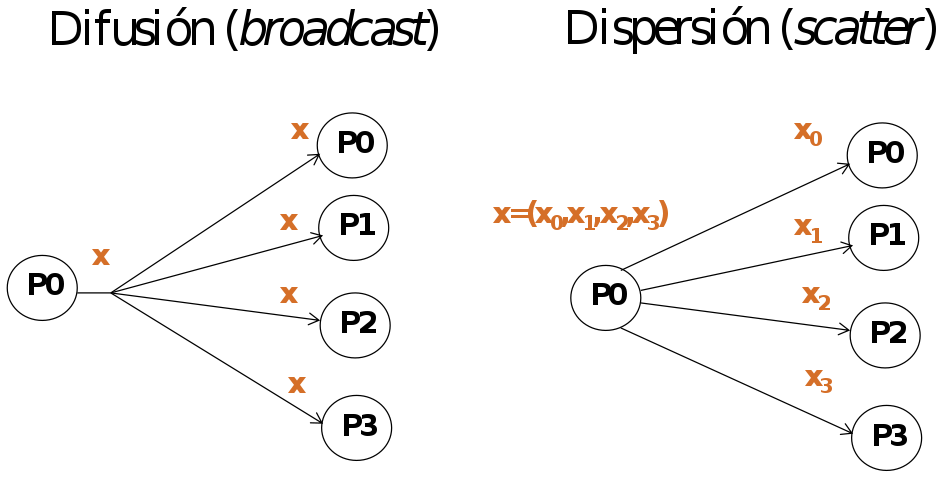
\includegraphics[width=0.5\textwidth]{29}
        \caption{Comunicación uno-a-todos}
        \label{comunicacion_uno_a_todos}
    \end{figure}

    \item \textcolor[rgb]{0.2,0.4,0.8}{\textbf{Comunicación todos-a-uno}}: todos los procesos en el grupo envían un mensaje a un único proceso (\hyperref[comunicacion_todos_a_uno]{Figura \ref*{comunicacion_todos_a_uno}}).
    \begin{enumerate}[$\longrightarrow$]
        \item \textcolor[rgb]{0.2,0.4,0.8}{\textbf{Reducción}}: los mensajes enviados se combinan en un sólo mensaje mediante algún operador. La operación de combinación suele ser conmutativa y asociativa.
        \item \textcolor[rgb]{0.2,0.4,0.8}{\textbf{Acumulación (\textit{gather})}}: los mensajes se reciben de forma concatenada en el receptor. El orden de concatenación depende del identificador del proceso.
    \end{enumerate}
    \begin{figure}[!h]
        \centering
        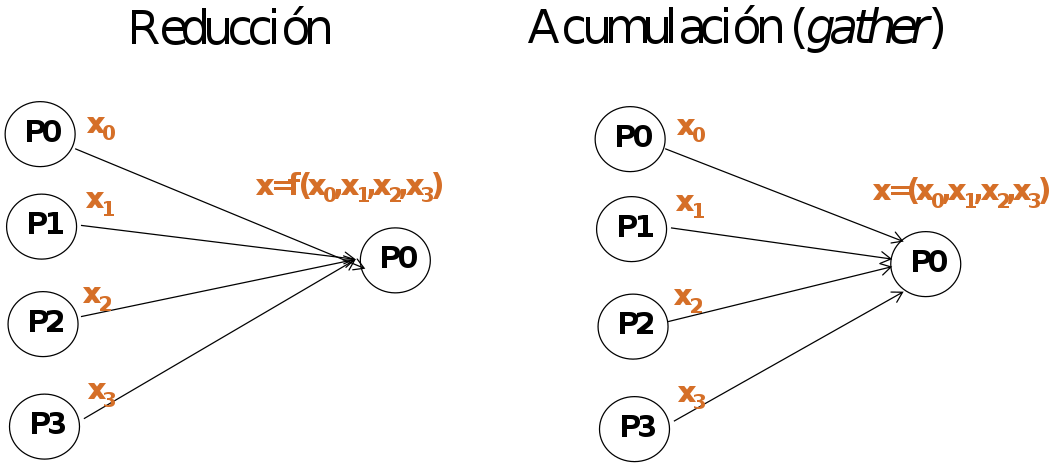
\includegraphics[width=0.5\textwidth]{30}
        \caption{Comunicación todos-a-uno}
        \label{comunicacion_todos_a_uno}
    \end{figure}
    \item \textcolor[rgb]{0.2,0.4,0.8}{\textbf{Comunicación múltiple uno-a-uno}}: hay componentes del grupo que envían un único mensaje y componentes que reciben un único mensaje (\hyperref[comunicacion_mult_uno_a_uno]{Figura \ref*{comunicacion_mult_uno_a_uno}}). Si todos los componentes del grupo envían y reciben, se implementa una \textbf{\textcolor[rgb]{0.2,0.4,0.8}{permutación}} (rotación, intercambio, barajes...). 
    \begin{figure}[!h]
        \centering
        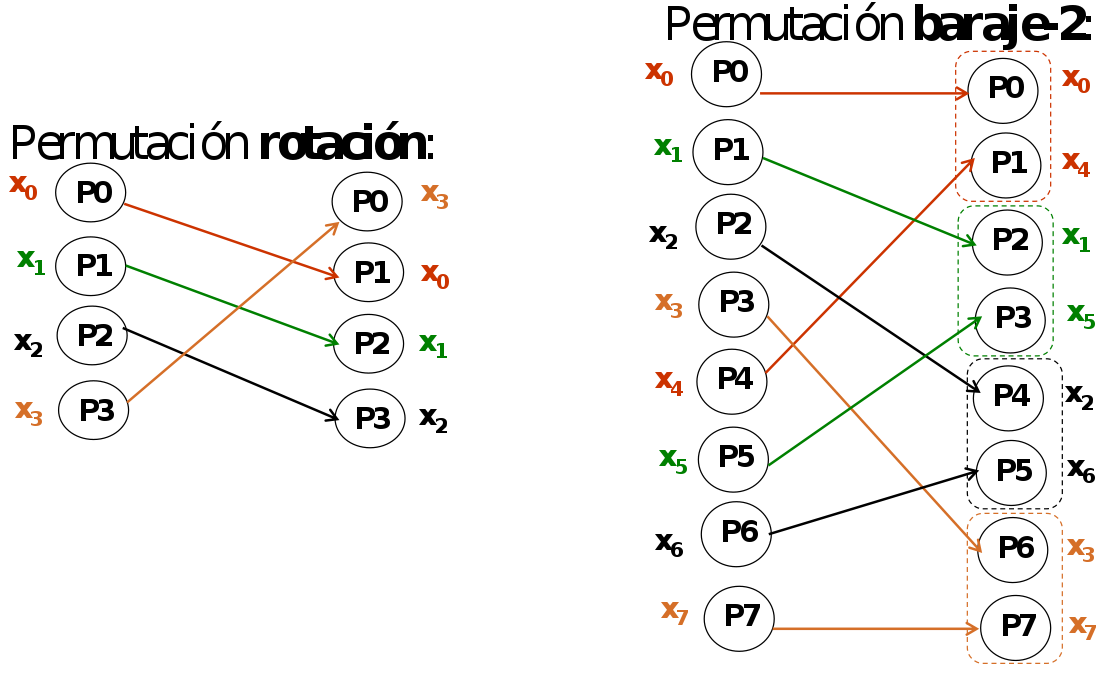
\includegraphics[width=0.5\textwidth]{28}
        \caption{Comunicación múltiple uno-a-uno}
        \label{comunicacion_mult_uno_a_uno}
    \end{figure}
    \item \textcolor[rgb]{0.2,0.4,0.8}{\textbf{Comunicación todos-a-todos}}: Todos los procesos del grupo ejecutan una comunicación \hyperref[uno_a_todos]{uno-a-todos} (\hyperref[comunicacion_todos_a_todos]{Figura \ref*{comunicacion_todos_a_todos}}). Cada proceso recibe $n$ mensajes, cada uno de un proceso diferente del grupo:
    \begin{enumerate}[$\longrightarrow$]
        \item \textcolor[rgb]{0.2,0.4,0.8}{\textbf{Todos-Difunden (\textit{all-broadcast})}}: todos los procesos realizan una difusión. Usualmente las $n$ transferencias recibidas por un proceso se concatenan en función del identificador del proceso que envía.
        \item \textcolor[rgb]{0.2,0.4,0.8}{\textbf{Todos-Dispersan (\textit{all-scatter})}}: todos los procesos concatenan diferentes transferencias. En el ejemplo de la \hyperref[comunicacion_todos_a_todos]{Figura \ref*{comunicacion_todos_a_todos}}, se ilustra una transposición de una matriz $4 \times 4$: el procesador $P_i$ dispersa la fila $i$ ($x_0, x_1, x_2, x_3$); tras la ejecución, el procesador $P_i$ tendrá la columna $i$ ($x_0, x_1, x_2, x_3$).
    \end{enumerate}
    \begin{figure}[!h]
        \centering
        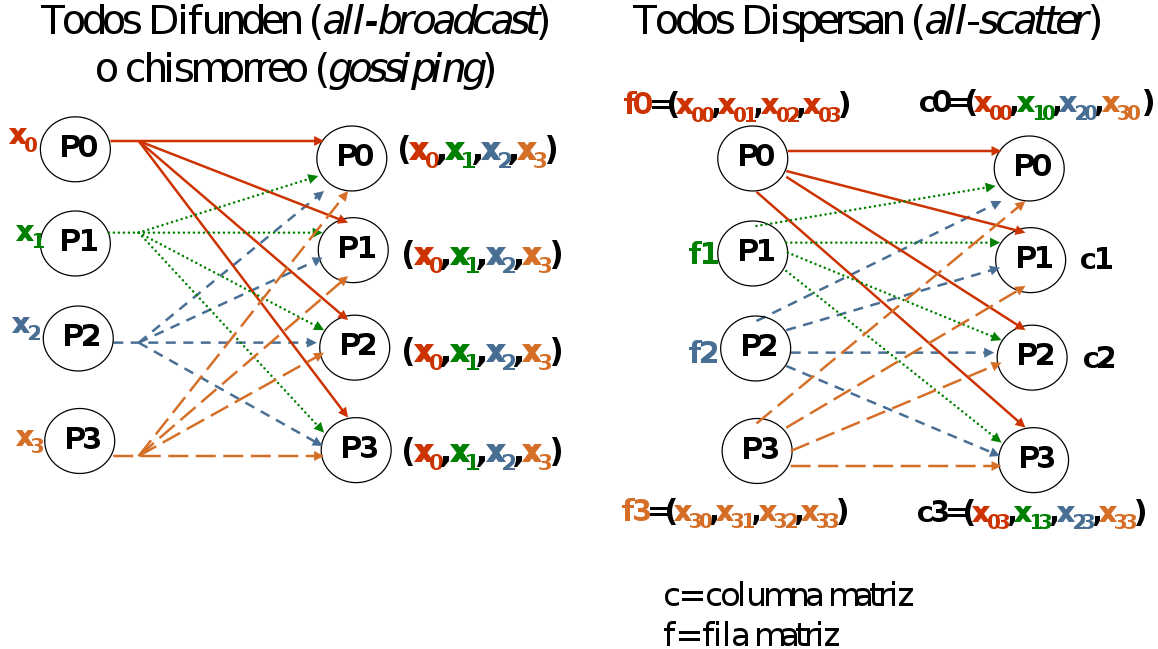
\includegraphics[width=0.5\textwidth]{31}
        \caption{Comunicación todos-a-todos}
        \label{comunicacion_todos_a_todos}
    \end{figure}
    \item \textcolor[rgb]{0.2,0.4,0.8}{\textbf{Servicios compuestos}}: hay servicios que resultan de una combinación de algunos de los anteriores, por ejemplo:
    \begin{enumerate}[$\longrightarrow$]
        \item \textcolor[rgb]{0.2,0.4,0.8}{\textbf{Todos combinan}}: el resultado de aplicar una reducción se obtiene en todos los procesos porque se realizan tantas reducciones como procesos (\hyperref[todos_combinan]{Figura \ref*{todos_combinan}})
        \begin{figure}[!h]
            \centering
            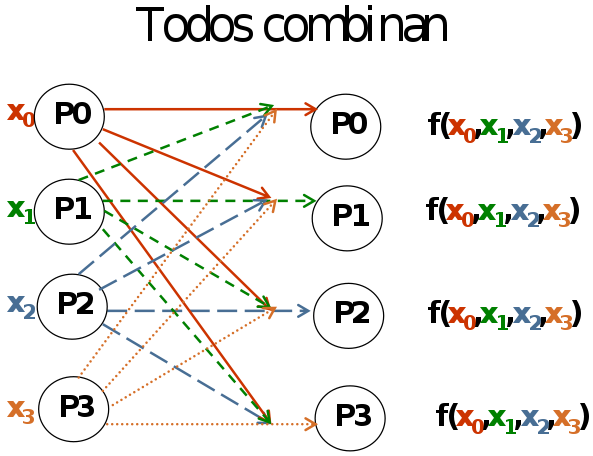
\includegraphics[width=0.3\textwidth]{32}
            \caption{Todos combinan}
            \label{todos_combinan}
        \end{figure}
        \item \textcolor[rgb]{0.2,0.4,0.8}{\textbf{Barrera}}: es un punto de sincronización en el flujo de control de un programa que todos los procesos de un grupo (no enmascarados) deben alcanzar para que cualquier proceso (no enmascarado) del grupo pueda continuar con la ejecución de la instrucción que hay tras la barrera.
        \item \textcolor[rgb]{0.2,0.4,0.8}{\textbf{Recorrido (\textit{scan})}}: todos los procesos envían un mensaje, recibiendo cada uno de ellos el resultado de reducir un conjunto de estos mensajes (\hyperref[recorrido]{Figura \ref*{recorrido}}). Con recorrido prefijo paralelo, el proceso $P_0$ se queda con el dato que él mismo ha enviado; $P_1$ recibe la reducción de dos mensajes $P_0$ y $P_1$; $P_2$ recibe la reducción de los mensajes de $P_0, P_1$ y $P_2$ y así sucesivamente. 
        \begin{figure}[!h]
            \centering
            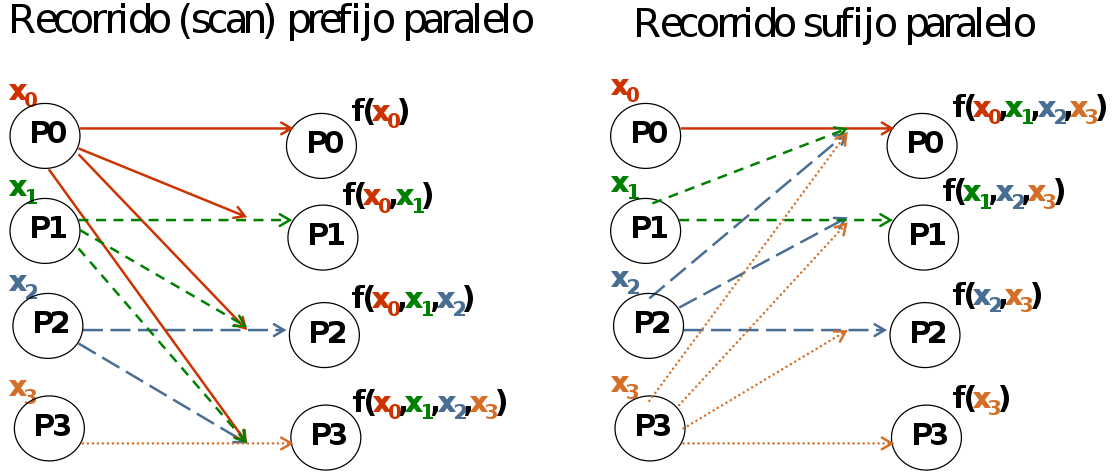
\includegraphics[width=0.5\textwidth]{33}
            \caption{Recorrido}
            \label{recorrido}
        \end{figure}
    \end{enumerate}
\end{enumerate}

\textcolor[rgb]{0.2,0.4,0.8}{\subsubsection{Ejemplo: comunicación colectiva en OpenMP}}
\begin{center}
\begin{tabular}{|>{\columncolor[rgb]{1,0.5,0.5}}c|c|p{10cm}|}
\hline
& & --- Claúsula \verb*|firstprivate| (desde thread 0) \\
\textcolor[rgb]{1,1,1}{\textbf{Uno-a-todos}} & Difusión & --- Directiva \verb*|single| con cláusula \verb*|copyprivate| \\
& & --- Directiva \verb*|threadprivate| y uso de la cláusula \verb*|copyin| en directiva \verb*|parallel| (desde thread 0) \\
\hline
\textcolor[rgb]{1,1,1}{\textbf{Todos-a-uno}} & Reducción & --- Claúsula \verb*|reduction| \\
\hline
\textcolor[rgb]{1,1,1}{\textbf{Servicios compuestos}} & Barreras & --- Directiva \verb*|barrier| \\
\hline
\end{tabular}
\end{center}

\textcolor[rgb]{0.2,0.4,0.8}{\subsubsection{Ejemplo: comunicación en MPI}}
\begin{center}
\begin{tabular}{|>{\columncolor[rgb]{1,0.5,0.5}}c|c|p{10cm}|}
\hline
\textcolor[rgb]{1,1,1}{\textbf{Uno-a-uno}} & Asíncrona & --- \verb*|MPI_Send()| / \verb*|MPI_Receive()| \\
\hline
\textcolor[rgb]{1,1,1}{\textbf{Uno-a-todos}} & Difusión & --- \verb*|MPI_Bcast()| \\
& Dispersión & --- \verb*|MPI_Scatter()| \\
\hline
\textbf{\textcolor[rgb]{1,1,1}{Todos-a-uno}} & Reducción & --- \verb*|MPI_Reduce()| \\
& Acumulación & --- \verb*|MPI_Gather()| \\
\hline
\textbf{\textcolor[rgb]{1,1,1}{Todos-a-todos}} & Todos difunden & --- \verb*|MPI_Allgather()| \\
\hline
\textbf{\textcolor[rgb]{1,1,1}{Servicios}} & Todos combinan & --- \verb*|MPI_Allreduce()| \\
\textbf{\textcolor[rgb]{1,1,1}{compuestos}} & Barreras & --- \verb*|MPI_Barrier()| \\
& Scan & --- \verb*|MPI_Scan()| \\
\hline
\end{tabular}  
\end{center}

\textcolor[rgb]{0.2,0.4,0.8}{\subsection{Estilos de programación y arquitecturas paralelas}}
Como se ve en la \hyperref[estilos_prog]{Figura \ref*{estilos_prog}}, cada estilo de programación paralela se implementa mejor en distintos tipos de computadores.


\begin{figure}[!h]
    \centering
    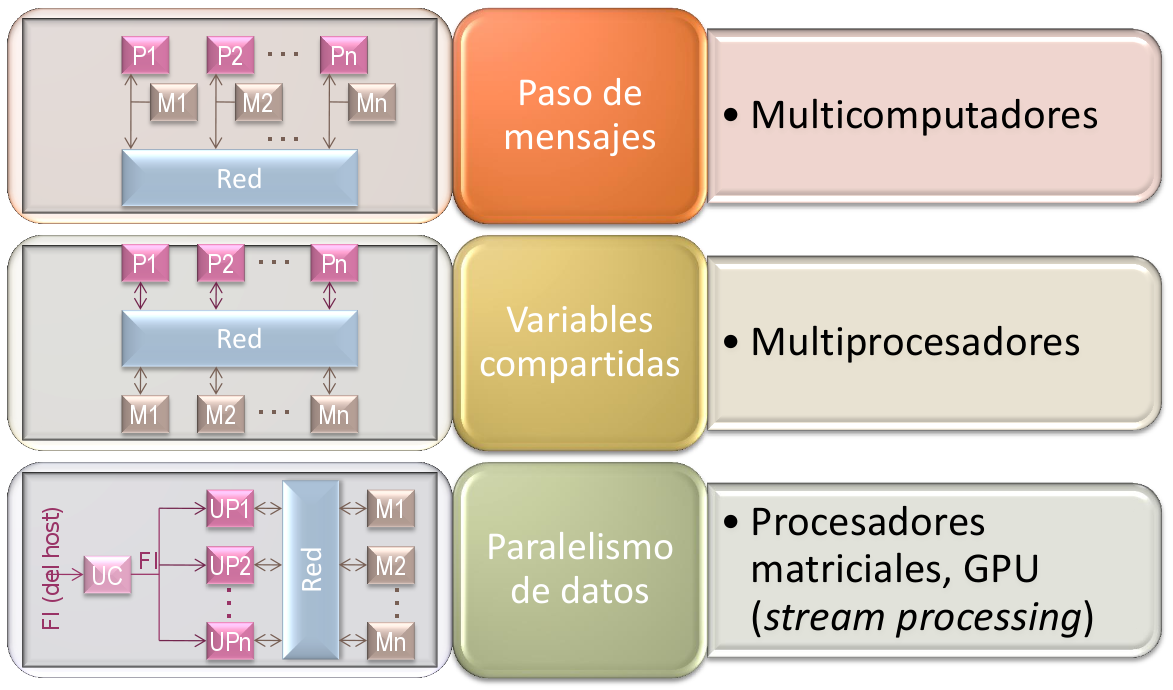
\includegraphics[width=0.7\textwidth]{34}
    \caption{Estilos de programación y arquitecturas paralelas}
    \label{estilos_prog}
\end{figure}

\textcolor[rgb]{0.2,0.4,0.8}{\subsubsection{Paso de mensajes}}
Con \textbf{\textcolor[rgb]{0.2,0.4,0.8}{paso de mensajes}} se supone que cada procesador en el sistema tiene su propio espacio de direcciones. Los mensajes llevan datos de una memoria a otra y se pueden usar para sincronizar procesos. Estos datos transferidos están duplicados en el sistema de memoria. 

Disponemos de varias herramientas como \textit{\textcolor[rgb]{0.2,0.4,0.8}{lenguajes de programación}} (Ada) o \textcolor[rgb]{0.2,0.4,0.8}{\textit{bibliotecas de funciones}} que actúan de interfaz al sistema de comunicaciones (MPI). 

Las funciones básicas de comunicación de paso de mensajes deben permitir la comunicación uno-a-uno entre procesos, con dos funciones:
\begin{enumerate}[\color{azul}{\bf $\heartsuit$}]
    \item \textcolor[rgb]{0.2,0.4,0.8}{\textit{Send (destino, datos)}}, donde $datos$ especifica la variable que contiene los datos a enviar.
    \item \textcolor[rgb]{0.2,0.4,0.8}{\textit{Receive (fuente, datos)}}, donde $datos$ especifica la variable dónde se guardarán los datos recibidos.
\end{enumerate}

Las transmisiones pueden ser:
\begin{enumerate}[\color{azul}{\bf $\heartsuit$}]
    \item \textcolor[rgb]{0.2,0.4,0.8}{\textit{Síncronas}}: el proceso que ejecuta el envío de datos queda bloqueado hasta que el destino ejecute la función para recibirlos correspondiente. igualmente, el proceso que ejecuta el receive queda bloqueado hasta que se ejecute el send correspondiente. Estas operaciones implementan las denominadas \textbf{\textcolor[rgb]{0.2,0.4,0.8}{citas}}
    \item \textcolor[rgb]{0.2,0.4,0.8}{\textit{Asíncronas}}: el send no deja bloqueado al proceso que lo ejecuta, generalmente se ofrece una implementación de receive que deja bloqueado el proceso hasta que se realice en correspondiente send. Para que el send sea no bloqueante debe usarse un buffer donde guardar los datos que se envían al destino.
\end{enumerate}

\textcolor[rgb]{0.2,0.4,0.8}{\subsubsection{Variables compartidas}}
Con \textcolor[rgb]{0.2,0.4,0.8}{\textbf{variables compartidas}}, los procesadores del sistema comparten el mismo espacio de direcciones, por eso no se necesita transferir datos, sino que se realizan transferencias con instrucciones del procesador implícitamente. Para sincronizar procesos el programador usa primitivas que ofrece el software.

Disponemos de varias herramientas como \textcolor[rgb]{0.2,0.4,0.8}{\textit{lenguajes de programación}} (Java), \textcolor[rgb]{0.2,0.4,0.8}{\textit{bibliotecas de funciones}} (PThread) y alternativas que usan lenguaje secuencial \textit{\textcolor[rgb]{0.2,0.4,0.8}{más directivas del compilador}} (OpenMP).

La comunicación entre procesos se realiza accediendo a variables compartidas. Las hebras pueden compartir variables globales pero los procesos no porque tienen espacio de direcciones independiente.

Las herramientas software ofrecen mecanismos para implementar sincronización como cerrojos, semáforos ó monitores. Estas herramientas sitúan al programador en distintos niveles de abstracción

\textcolor[rgb]{0.2,0.4,0.8}{\subsubsection{Paralelismo de datos}}
Con \textcolor[rgb]{0.2,0.4,0.8}{\textbf{paralelismo de datos}}, las mismas operaciones se ejecutan en paralelo en múltiples unidades de procesamiento de forma que cada unidad aplica la operación a un conjunto de datos distinto. Sólo soporta paralelismo a nivel de bucle y la sincronización está implícita. 

Permite aprovechar el paralelismo de datos en aplicaciones que organizan sus datos en vectores o matrices. El programador no debe preocuparse de las sincronizaciones pues están implícitas y las genera el compilador.

Los lenguajes de paralelismo de datos como C* aparecieron ligados a procesadores matriciales (arquitectura SIMD). 

\textcolor[rgb]{0.2,0.4,0.8}{\subsection{Estructuras típicas de códigos paralelos}}
\textcolor[rgb]{0.2,0.4,0.8}{\subsubsection{Dueño-Esclavo (master-slave) o Granja de tareas (task-farming)}}
Se distingue un proceso dueño y múltiples esclavos. El dueño se encarga de distribuir las tareas de un conjunto (granja) entre el grupo de esclavos y de ir recolectando los resultados parciales que van calculando para obtener el resultado final. No suele haber comunicación entre los esclavos (\hyperref[master_slave]{Figura \ref*{master_slave}}).

\begin{figure}[!h]
    \centering
    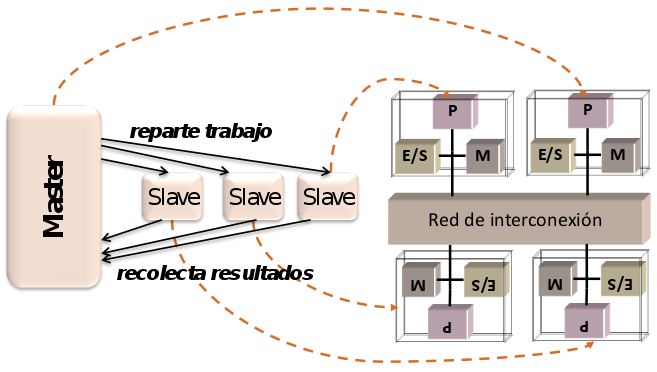
\includegraphics[width=0.5\textwidth]{35}
    \caption{Esquema del dueño-esclavo}
    \label{master_slave}
\end{figure}

Si todos los esclavos ejecutan el mismo código, se puede hacer un programa para el dueño y otro para el esclavo (modo mixto MPMD-SPMD). También pueden juntarse ambos en un único programa (SPMD).

El reparto de trabajo puede hacerse de forma dinámica (durante la ejecución) ó de forma estática (por el programador). De forma estática sabemos a priori lo que va a hacer cada esclavo y el dueño sólo se encarga de reunir resultados.

La escabilidad dependerá del número de esclavos y de su comunicación con el dueño. Para aumentar la escabilidad puede haber múltiples dueños cada uno con un subconjunto de esclavos.

Esta estructura de la \hyperref[master_slave]{Figura \ref*{master_slave}} es a nivel de procesos

\textcolor[rgb]{0.2,0.4,0.8}{\subsubsection{Cliente-Servidor}}
\begin{figure}[!h]
    \centering
    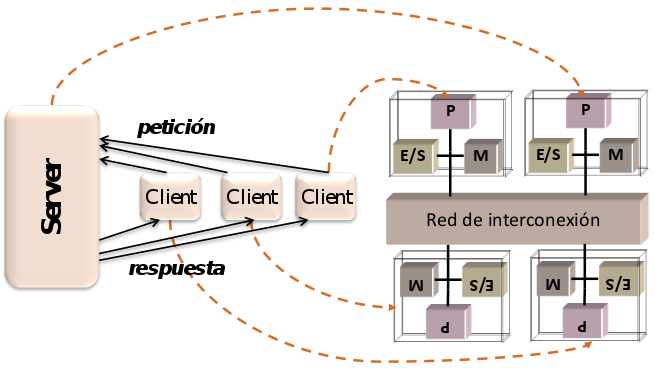
\includegraphics[width=0.5\textwidth]{36}
    \caption{Esquema del cliente-servidor}
    \label{cliente_servidor}
\end{figure}

Tiene una estructura parecida al dueño-esclavo pero cambia el sentido de las flechas. Los clientes envían una petición al servidor y éste les devuelve la respuesta.

\textcolor[rgb]{0.2,0.4,0.8}{\subsubsection{Descomposición de dominio o descomposición de datos}}
\begin{figure}[!h]
    \centering
    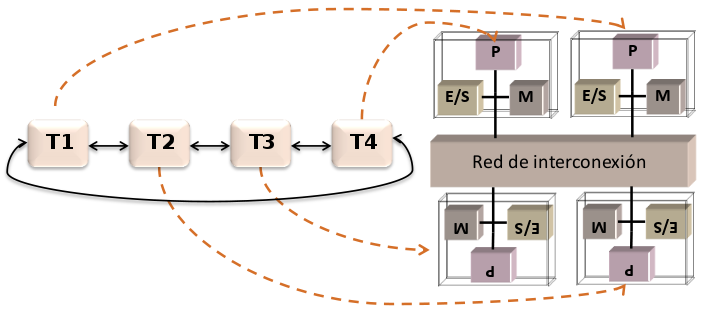
\includegraphics[width=0.5\textwidth]{37}
    \caption{Esquema de la descomposición de datos}
    \label{descomposicion_datos}
\end{figure}

Se usa en problemas en los que se opera con estructuras de datos grandes. Éstas se dividen en partes y con esta división se derivan las tareas paralelas. Éstas suelen realizar las mismas operaciones (\hyperref[descomposicion_datos]{Figura \ref*{descomposicion_datos}}). Los algoritmos con imágenes, por ejemplo, admiten descomposición de datos (\hyperref[filtrado_de_imagen]{Figura \ref*{filtrado_de_imagen}}).

Para hacer el filtrado de una imagen cada pixel se sustituye por una combinación de los píxeles que tiene alrededor y él mismo. En el ejemplo se ve una imagen de $4 \times 4$ px. Para decodificar la imagen repartimos el trabajo por columnas, cada columna se asigna a un flujo de control distinto (en este caso tendremos cuatro threads). Para obtener el filtrado de un píxel necesitamos datos presentes en otras columnas. Las comunicaciones necesarias se harían por filas y columnas (los datos de las columnas los tiene ya ese thread por tanto sólo se comunicaría un thread con el anterior y el posterior en la matriz), por tanto, los threads envían y reciben de otros dos threads.

El código para hacer esto se ve en la \hyperref[filtrado_de_imagen]{Figura \ref*{filtrado_de_imagen}}.

\begin{figure}[!h]
    \centering
    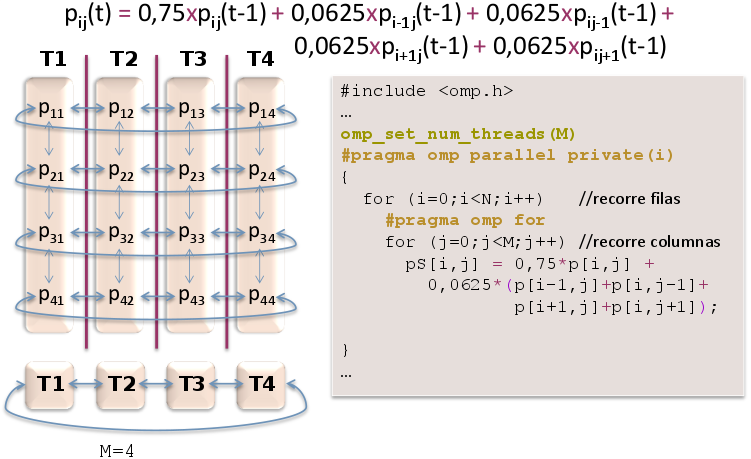
\includegraphics[width=0.5\textwidth]{38}
    \caption{Ejemplo: filtrado de imagen}
    \label{filtrado_de_imagen}
\end{figure}

Los procesos pueden englobar varias tareas. Suelen ejecutar el mismo código (SPMD) aunque cada uno trabaja sobre un conjunto de datos diferente. Puede haber comunicaciones entre procesos, de hecho, si no hay comunicación entre procesos se conoce como \textit{\textcolor[rgb]{0.2,0.4,0.8}{embarrasing parallel computation}}.

\textcolor[rgb]{0.2,0.4,0.8}{\subsubsection{Estructura segmentada (pipeline) o flujo de datos}}
\begin{figure}[!h]
    \centering
    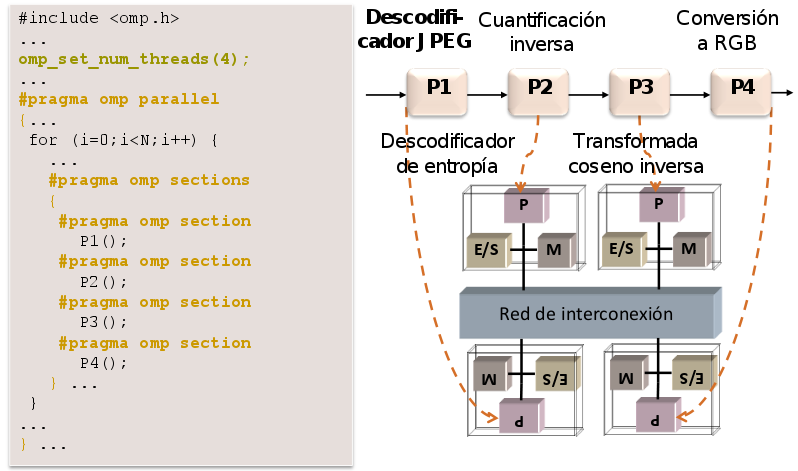
\includegraphics[width=0.5\textwidth]{39}
    \caption{Esquema de flujo de datos con ejemplo de decodificador JPEG}
    \label{flujo_datos}
\end{figure}

Se usa para aplicar a un flujo de datos en secuencia distintas funciones (paralelismo de tareas). La estructura de los procesos y de las tareas es la de un cauce segmentado (\hyperref[flujo_datos]{Figura \ref*{flujo_datos}}). Cada proceso ejecuta, por tanto, código distinto (MPDP). 

Por ejemplo, en un decodificador de imágenes JPEG, se aplica en secuencia a bloques de $8 \times 8$ píxeles de una imagen de entrada, las siguientes funciones: decodificación de entropía, cuantificación inversa, transformada del coseno inversa y conversión RGB. Por tanto el decodificador se podría implementar con cuatro procesos en una estructura segmentada.

No se puede aplicar una descomposición de dominio porque cada bloque necesita los datos que se han calculado del bloque anterior.

Para traducir esto a código y ejecutar en paralelo las distintas etapas usamos la directiva de OpenMP \verb*|section|.

\textcolor[rgb]{0.2,0.4,0.8}{\subsubsection{Divide y vencerás (divide and conquer) ó descomposición recursiva}}
\begin{figure}[!h]
    \centering
    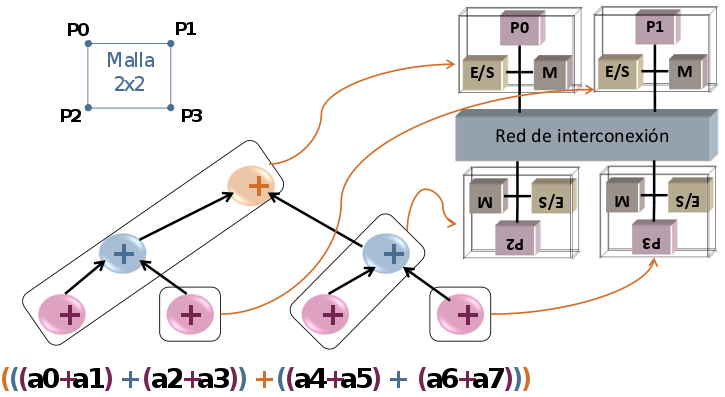
\includegraphics[width=0.5\textwidth]{40}
    \caption{Esquema de divide y vencerás}
    \label{divide_conquer}
\end{figure}
Esta estructura se utiliza cuando un problema se puede dividir en subproblemas independientes. Si los subproblemas se pueden dividir, lo harán también, recursivamente. Las tareas presentan una estructura en forma de árbol y no habrá comunicación interacciones entre los hijos del mismo padre. (\hyperref[divide_conquer]{Figura \ref*{divide_conquer}}).

Los programas secuenciales recursivos (paralelismo de tareas) y la descomposición de los datos de un problema recursivamente (paralelismo de datos) también tienen divide y vencerás. Por ejemplo, un vector cuyos datos se van a sumar puede descomponerse en vectores la mitad de componentes hasta llegar a vectores de dos componentes sólo.

La asignación de tareas puede hacerse asignando a cada proceso una tarea o dependiendo de la red de interconexión de la máquina, para disminuir el número de enlaces de la red que se utilizarán para cada comunicación.

En la \hyperref[divide_conquer]{Figura \ref*{divide_conquer}} se descompone la suma de 8 números, en primer lugar en la suma de cuatro números y, en el siguiente nivel del árbol, en la suma de dos números. Los resultados de cada nivel se deben sumar para obtener la combinación lineal del nivel superior.

El número mínimo de procesadores que necesitamos para tener paralelismo (para obtener paralelismo en una aplicación\footnote{GRADO DE PARALELISMO: número máximo de flujos de control que un programa puede ejecutar en paralelo, donde para que la ejecución de nuestras tareas sea lo más eficiente posible. No puede superar este número.}) viene dado por el número de hojas del árbol.

\textcolor[rgb]{0.2,0.4,0.8}{\section{Proceso de paralelización}}
Para obtener una versión paralela de una aplicación se podrían seguir los siguientes pasos:
\begin{enumerate}[\color{azul}{\bf $\heartsuit$}]
    \item \textcolor[rgb]{0.2,0.4,0.8}{\textbf{Descomponer} la aplicación en tareas independientes}
    \item \textcolor[rgb]{0.2,0.4,0.8}{\textbf{Asignar} tareas a procesos o a hebras}
    \item \textcolor[rgb]{0.2,0.4,0.8}{\textbf{Redactar} código paralelo}
    \item \textcolor[rgb]{0.2,0.4,0.8}{\textbf{Evaluar} prestaciones}
\end{enumerate}

\textcolor[rgb]{0.2,0.4,0.8}{\subsection{Descomposición en tareas independientes}}
En esta etapa se buscan unidades de trabajo independientes que, junto con los datos que utilizan, formarán las \textit{\textcolor[rgb]{0.2,0.4,0.8}{tareas}}. Se deben representar mediante un grafo dirigido las dependencias entre las tareas: los arcos en el grafo representan el flujo de datos y de control, y los vértices, tareas. Así, podemos detectar las tareas independientes y facilitarnos la vida en la etapa de asignación.

Esta búsqueda se realiza a partir de un código secuencial en dos niveles de abstracción:
    \begin{figure}[!h]
        \centering
        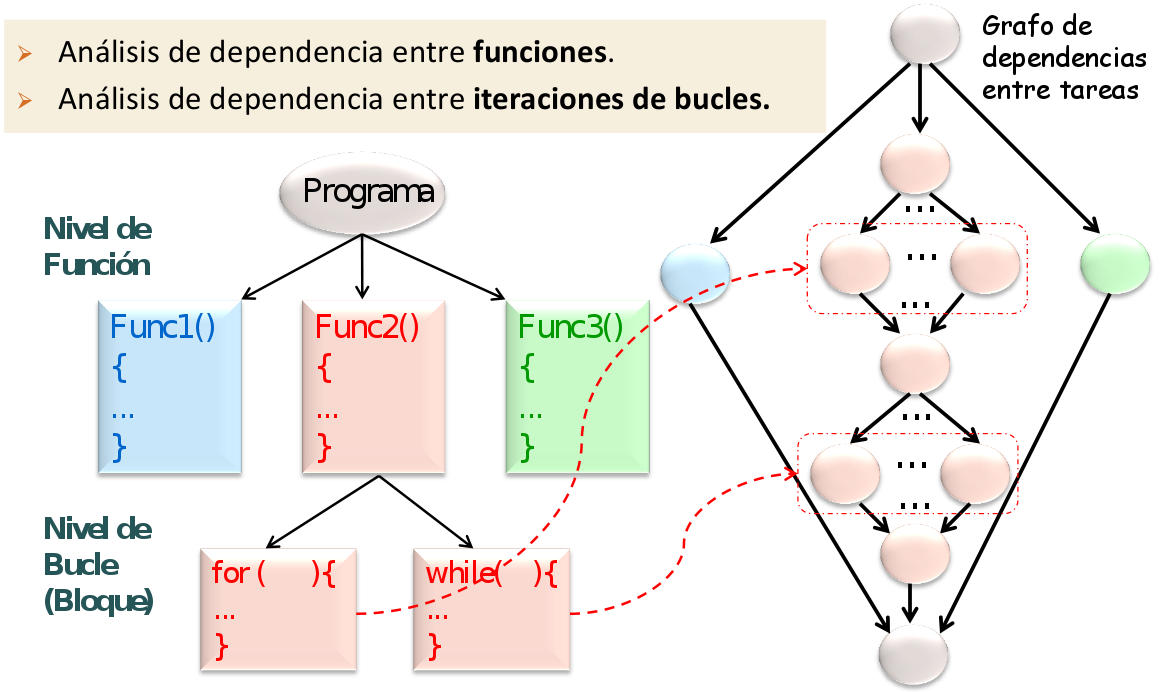
\includegraphics[width=0.7\textwidth]{41}
        \caption{Descomposición en tareas}
        \label{destareas}
    \end{figure}
\begin{enumerate}[\color{azul}{\bf $\heartsuit$}]
    \item \textcolor[rgb]{0.2,0.4,0.8}{\textbf{Nivel de función}}: analizando las dependencias entre las funciones del código encontramos las que son independientes o las que se pueden hacer independientes y, por tanto, ejecutarse en paralelo. En el ejemplo de la \hyperref[destareas]{Figura \ref*{destareas}} se ha encontrado que las tres funciones son independientes.
    \item \textcolor[rgb]{0.2,0.4,0.8}{\textbf{Nivel de bucle}}: analizando las iteraciones de los bucles dentro de una función, podemos encontrar si son o se pueden hacer independientes (es decir, asegurarnos de que no haya dependencias RAW entre las iteraciones del bucle). Con el análisis de los bucles podemos detectar el paralelismo de datos. Además, si una función tiene varios bucles podemos analizar la dependencia entre ellos. En el ejemplo de la \hyperref[destareas]{Figura \ref*{destareas}}, una de las funciones consta de dos bucles y con el grafo de dependencias se ha encontrado que son independientes las iteraciones de cada bucle, en cambio, la salida del bucle for es usada en el bucle while, por eso ambos ciclos están a diferente nivel en el grafo.
\end{enumerate}

Si partimos de la definición de la aplicación se puede extraer paralelismo de tareas (\textcolor[rgb]{0.2,0.4,0.8}{\textit{task-parallelism}}). Para extraer paralelismo de datos (\textcolor[rgb]{0.2,0.4,0.8}{\textit{data parallelism}}) se podría estudiar dentro de cada función la estructura de los datos y realizar una descomposición recursiva.

\textcolor[rgb]{0.2,0.4,0.8}{\subsubsection{Ejemplo de cálculo $\pi$: descomposición en tareas independientes}}
Para paralelizar el cálculo de $\pi$ se puede partir de una versión secuencial o un planteamiento para que el problema se preste a paralelización.

Podemos definir el cálculo de $\pi$  como un problema de integración numérica, $\pi$ es la integral en el intervalo $[0,1]$ de la derivada del arco tangente de $x$ que es $\frac{\pi}{4}$:

\begin{displaymath}
\left. \begin{array}{lll}
arctg'(x)=\frac{1}{1+x^2}\\
arctg(1)=\frac{\pi}{4}\\
arctg(0)=0
\end{array} \right\} \Rightarrow \int_0^1 \frac{1}{1+x^2} = arctg(x)\mid_0^1 = \frac{\pi}{4} - 0
\end{displaymath}

$(i+0.5)\cdot A$ es la altura del rectángulo del que estamos calculando el área y $A$ es la base de dicho rectángulo.

\begin{displaymath}
\pi = 4 \cdot \int_0^1 \frac{1}{1+x^2} \approx 4 \cdot \sum_{i=0}^{intervalos-1} Ancho \cdot \frac{1}{1+[(i+0.5)\cdot A]^2}
\end{displaymath}

La fórmula que implementamos en el código secuencial es:
\begin{displaymath}
\pi = A \cdot \sum_{i=0}^{intervalos-1} \frac{4}{1+[(i+0.5)\cdot A]^2}
\end{displaymath}
Si sacamos el ancho fuera obtenemos el área con mayor precisión y con menor número de intervalos. Así, calculamos la altura de cada rectángulo y al final, multplicamos toda la sumatoria por el ancho del rectángulo.

El área de la derivada del arcotangente en $[0,1]$ se aproxima dividiendo el intervalo en subintervalos, calculando el área de cada subintervalo y sumando las áreas obtenidas en cada subintervalo. El error será menor cuanto mayor sea el número de subintervalos.

El cálculo del área de los diferentes intervalos es independiente, por lo que podemos repartir estos cálculos en un conjunto de procesadores. Si se divide el intervalo en 100 y disponemos de 10 procesadores, a cada procesador podemos asignarle el cálculo de 10 áreas.

Otra alternativa es partir de una versión secuencial. Esta versión secuencial calcula $\pi$ utilizando rectángulos en los que la altura es el valor de la derivada de la arcotangente en el punto medio. Usa un bucle \verb*|for| que escribe siempre en la misma variable $sum$, pero esta dependencia se puede eliminar suponiendo que cada hebra escribirá en una variable $sum$ distinta:\\[0.2cm]



\begin{minipage}{0.5\textwidth}
\begin{minted}[linenos, frame=single, label={Código secuencial}]{c}
int main (int argc, char **argv) {
    double ancho, sum=0;
    int intervalos, i;

    // Primer nodo del grafo 
    // y primer nivel
    intervalos = atoi(argv[1]);
    ancho = 1.0/(double)intervalos;

    // Segundo y tercer nodo 
    // del grafo, en el segundo nivel
    for (i=0;i<intervalos;i++) {
        x = (i+0.5)*ancho;
        sum = sum + 4.0/(1.0+x*x);
    }

    // Cuarto nodo del grafo, 
    // en el tercer nivel
    sum *= ancho;

    return 0;
}
\end{minted}
\end{minipage}
\begin{minipage}{0.5\textwidth}
\begin{minted}[frame=single, label={Código con el paralelismo extraído}]{c}
#include <omp.h>
#define NUM_THREADS 4
int main (int argc, char **argv) {
    double ancho, sum=0;
    int intervalos, i;

    intervalos = atoi(argv[1]);
    ancho = 1.0/(double)intervalos;
    omp_set_num_threads(NUM_THREADS);

#pragma omp parallel
{
    #pragma omp for
    for (i=0;i<intervalos;i++) {
        x = (i+0.5)*ancho;
        sum = sum + 4.0/(1.0+x*x);
    }
}
    sum *= ancho;

    return 0;
}
\end{minted}
\end{minipage}

\textcolor[rgb]{0.2,0.4,0.8}{\subsection{Asignar tareas a procesos o hebras}}
Se realiza la asignación de las tareas del grado de dependencia a procesos y hebras. En general, no es conveniente asignar más de un proceso o hebra por procesador en una misma aplicación, por lo que la asignación a procesos y hebras (\textit{\textcolor[rgb]{0.2,0.4,0.8}{scheduling}}) está asignada con la asignación/mapeo de procesadores (\textcolor[rgb]{0.2,0.4,0.8}{\textit{mapping}}), incluso se puede realizar la asignación asociando los procesos/hebras a procesadores concretos. 

La granularidad de los procesos y hebras dependerá de:
\begin{enumerate}[\color{azul}{\bf $\heartsuit$}]
    \item Del número de procesadores que haya, ya que cuanto mayor sea su número menos tareas se asignarán a cada proceso. No se recomienda tener más threads que cores porque sino, perdemos tiempo comunicando threads de un mismo core y es más eficiente asignar el trabajo de esas dos threads a uno sólo y ejecutarlo en un core.
    \item Del tiempo de comunicación y sincronización, ya que el tiempo de ejecución paralelo no sólo depende del tiempo que supone la ejecución en paralelo de las tareas, sino que también depende del tiempo de comunicación y sincronización entre procesos/hebras. Para reducir este tiempo se asignan varias tareas a un mismo proceso/hebra y así reducir las interacciones. Si replicamos una tarea en todos los threads (que todos los threads ejecuten el mismo cálculo en vez de que lo ejecute uno y envíe el resultado al resto) disminuimos tiempo de comunicación y sincronización y podemos conseguir mayor velocidad.
\end{enumerate}

La asignación debería \textit{\textcolor[rgb]{0.2,0.4,0.8}{repartir la carga}} optimizando la \textcolor[rgb]{0.2,0.4,0.8}{\textit{comunicación y sincronización}}, de forma que todos los procesadores empiecen y terminen a la vez, es decir, no deben hacerse esperar los unos a los otros.

En el grafo de tareas, éstas representan tiempo de cálculo, y los arcos, tiempo de comunicación y sincronización. Para realizar la asignación y cumplir estos objetivos, conviene saber la \textcolor[rgb]{0.2,0.4,0.8}{\textit{arquitectura}} en la que se va a ejecutar la aplicación y conocer el tiempo de ejecución de cada tarea y de las comunicaciones/sincronizaciones entre ellas.

El equilibrado depende de:
\begin{enumerate}[\color{azul}{\bf $\heartsuit$}]
    \item \textcolor[rgb]{0.2,0.4,0.8}{\textbf{La arquitectura}}:
    \begin{enumerate}[$\longrightarrow$]
        \item \textcolor[rgb]{0.2,0.4,0.8}{\textbf{Heterogénea}}: consta de componentes con diferentes prestaciones, por lo que un buen equilibrado debería asignar más trabajo a los nodos más rápidos. Cuesta más trabajo asignar el trabajo para que todos empiecen y terminen a la vez.
        \item \textcolor[rgb]{0.2,0.4,0.8}{\textbf{Homogénea}}: Todos los nodos son iguales, con la misma velocidad y usando las mismas herramientas de programación. hay dos subtipos
        \begin{itemize}
            \item \textit{\textcolor[rgb]{0.2,0.4,0.8}{Uniforme}}: la comunicación de los procesadores con la memoria (multiprocesadores) o entre sí (multicomputadores) supone el mismo tiempo sean cuales sean los nodos que intervienen. En esta arquitectura no tiene mucha influencia el no considerar la arquitectura, aunque la distribución de las tareas de forma que las tareas de cada procesador estén en módulos de memoria distintos reduce las colisiones.
            \item \textcolor[rgb]{0.2,0.4,0.8}{\textit{No Uniforme}}: la asignación de tareas de forma que se minimice el tiempo de comunicación y sincronización es más difícil. Para mejorar el tiempo de ejecución se pueden eliminar transferencias a través de la red asignando tareas al mismo procesador y disminuir las distancias que se atraviesan en las transferencias.
        \end{itemize}
    \end{enumerate}
    \item \textcolor[rgb]{0.2,0.4,0.8}{\textbf{La aplicación/descomposición}}: porque hay aplicaciones en las que las tareas no tardan todas lo mismo, aunque sean iteraciones de un bucle.
\end{enumerate}

La asignación de tareas a procesadores se puede realizar de dos formas:
\begin{enumerate}[\color{azul}{\bf $\heartsuit$}]
    \item \textcolor[rgb]{0.2,0.4,0.8}{\textbf{Estática}}: en tiempo de compilación (implícita) o al escribir el programa (explícita).
    \item \textcolor[rgb]{0.2,0.4,0.8}{\textbf{Dinámica}}: en tiempo de ejecución. Su ventaja es que permite evitar repartos estáticos complejos, especialmente cuando no se conoce el número de tareas que se van a ejecutar antes de la ejecución, y permite que acabe una aplicación aunque falle un procesador. Aunque consume un tiempo extra de comunicación y sincronización. Aun sabiendo el número de tareas a ejecutar al programador puede resultarle más cómodo usar asignación dinámica para conseguir un buen equilibio, por ejemplo, cuando tenemos una arquitectura heterogénea/no uniforme/las tareas no tardan lo mismo, ya que se va asignando trabajo conforme se van terminando las tareas.
\end{enumerate}

Normalmente se deja al sistema operativo el mapeo de threads (\textcolor[rgb]{0.2,0.4,0.8}{\textit{light process}}). Lo puede hacer el entorno o sistema en tiempo de ejecución (\textcolor[rgb]{0.2,0.4,0.8}{\textit{runtime system}} de la herramienta de programación) aunque el programador puede influir.

Por ejemplo, en el filtrado de una imagen, se puede dividir el proceso en columnas (\hyperref[filtrado_de_imagen]{Figura \ref*{filtrado_de_imagen}}) o en filas (\hyperref[fil_img_filas]{Figura \ref*{fil_img_filas}}) y la asignación a procesadores, como tenemos en ambos casos cuatro tareas y cuatro procesadores, será de una tarea para cada procesador. Además, intentaremos al hacer el mapeo que procesadores cercanos tengan tareas que se comuniquen entre sí para que las comunicaciones y sincronizaciones sean más eficientes, ya que tenemos una arquitectura homogénea no uniforme.

\begin{figure}[!h]
\centering
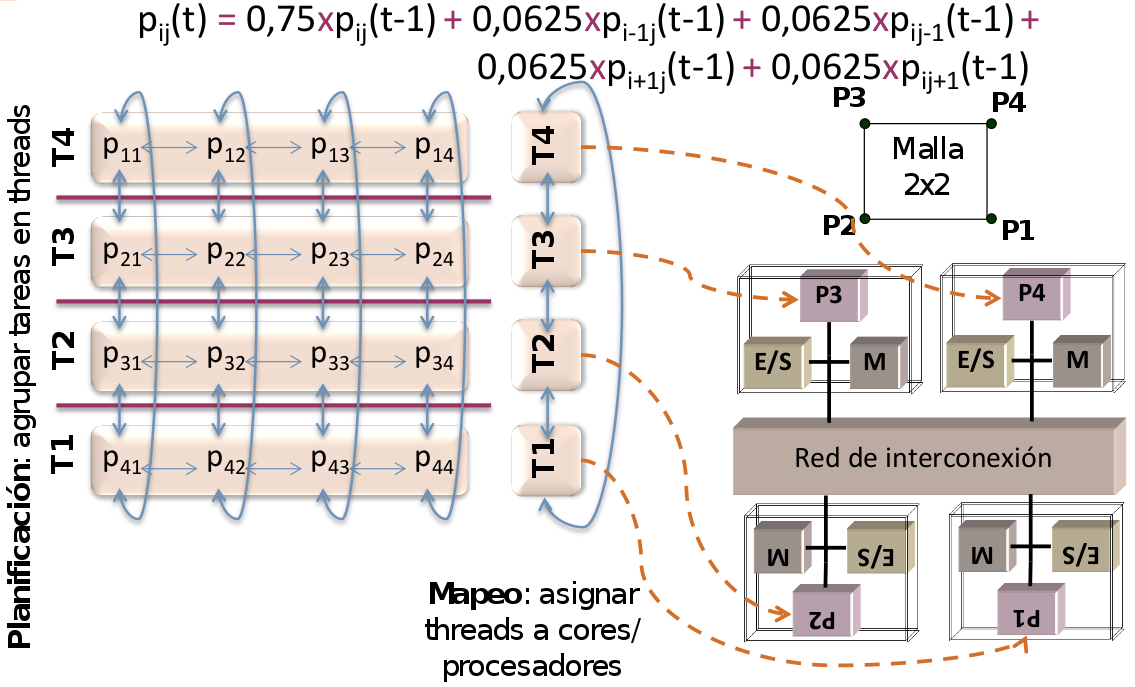
\includegraphics[width=0.7\textwidth]{42}
\caption{Filtrado de imagen por filas}
\label{fil_img_filas}
\end{figure}

Entonces, dependiendo de si repartimos el trabajo por columnas o por filas, tendremos los siguientes códigos paralelos:

\begin{minipage}{0.55\textwidth}
\usemintedstyle{perldoc}
\begin{minted}
[
linenos,
frame=single,
label={Descomposición en columnas},
]
{c}
#include<omp.h>
omp_set_num_threads(M)
#pragma omp parallel private(i)
{
    for (i=0;i<N;i++) {
        #pragma omp for
        for (j=0;j<M;j++) {
            pS[i,j]=0.75*p[i,j]+
                0.0625*(p[i-1,j]+p[i,j-1]+
                        p[i+1,j]+p[i,j+1]);
        }
    }
}
\end{minted}
\end{minipage}
\begin{minipage}{0.55\textwidth}
\usemintedstyle{manni}
\begin{minted}
[
frame=single,
label={Descomposición en filas},
]
{c}
#include<omp.h>
omp_set_num_threads(N)
#pragma omp parallel private(j)
{
    #pragma omp for
    for (i=0;i<N;i++) {
        for (j=0;j<M;j++) {
            pS[i,j]=0.75*p[i,j]+
                0.0625*(p[i-1,j]+p[i,j-1]+
                        p[i+1,j]+p[i,j+1]);
        }
    }
}
\end{minted}
\end{minipage}

El siguiente código es un ejemplo de asignación estática de paralelismo de tareas y datos en OpenMP:

\begin{minted}[linenos]{c}
void Func1() {...}
void Func2() {...
    #pragma omp parallel for schedule(static)
    for (i=0;i<N;i++)
        // codigo para i
...}
void Func3() {...}
int main () {
    #pragma omp parallel sections
    {
        #pragma omp section
            Func1();
        #pragma omp section
            Func2();
        #pragma omp section
            Func3();
    }
    ...
}
\end{minted}

Para repartir el trabajo nosotros mismos podemos usar en vez del \verb*|sections|, el identificador del thread. Así haríamos la asignación estática y explícita. Tal y como está en el código, como lo hace la herramienta de programación, es estática pero implícita.

Cada hebra ejecutará las funciones \verb*|Func1|, \verb*|Func2| y \verb*|Func3| en secuencial, pero las tres se ejecutarán en paralelo. Dentro de \verb*|Func2| se ejecurará el bucle for en paralelo, es decir, la hebra que ejecute \verb*|Func2| tendrá otras subhebras.

\begin{figure}[!h]
    \centering
    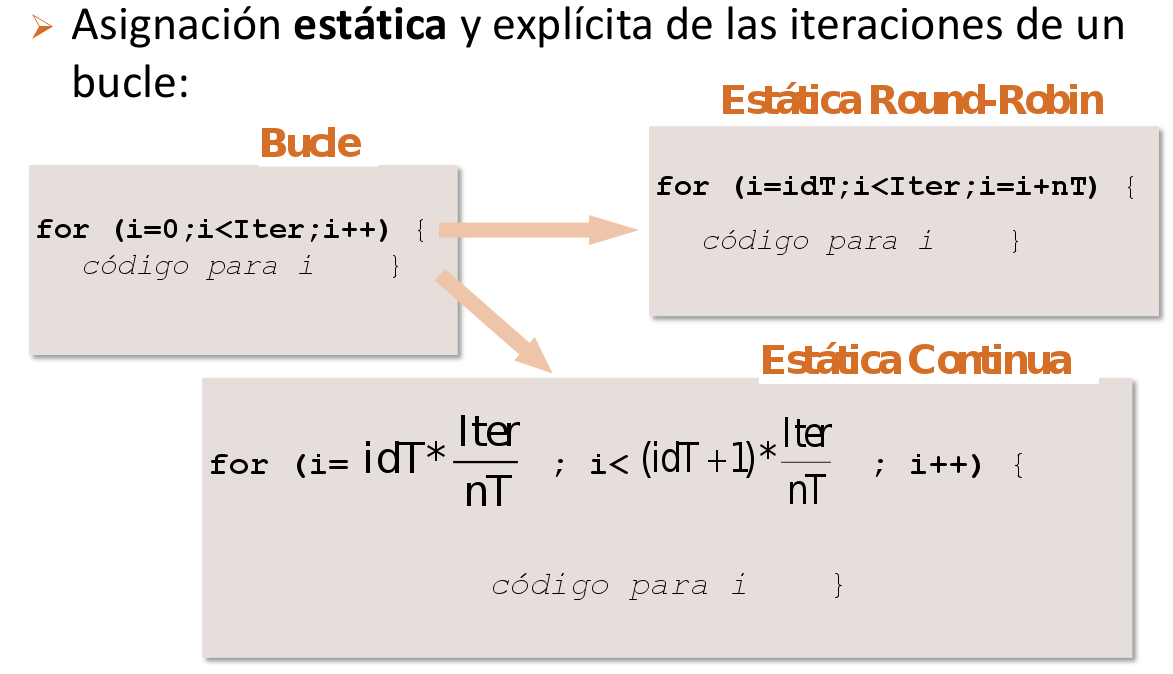
\includegraphics[width=0.7\textwidth]{43}
    \caption{Asignación estática explícita de las tareas de un bucle a procesos.}
    \label{tipos_estatica_asig}
\end{figure}

En la \hyperref[tipos_estatica_asig]{Figura \ref*{tipos_estatica_asig}} se pueden ver dos alternativas que el programador puede utilizar explícitamente para asignar las iteraciones de un bucle a procesos de forma estática. En la asignación \textcolor[rgb]{0.2,0.4,0.8}{\textit{round-robin}}, iteraciones consecutivas del bucle se asignan a procesos consecutivos (con identificador consecutivo). En el otro ejemplo se asignan iteraciones consecutivas al mismo proceso. 

Estas asignaciones serían explícitas porque las hace el programador variando los límites del bucle for.

En el ejemplo de $\pi$, sería mejor asignar las tareas consecutivas al mismo thread para no perder precisión al sumar los resultados, ya que la números en coma flotante con exponentes dispares puede hacer que perdamos decimales.

\begin{figure}[!h]
\centering
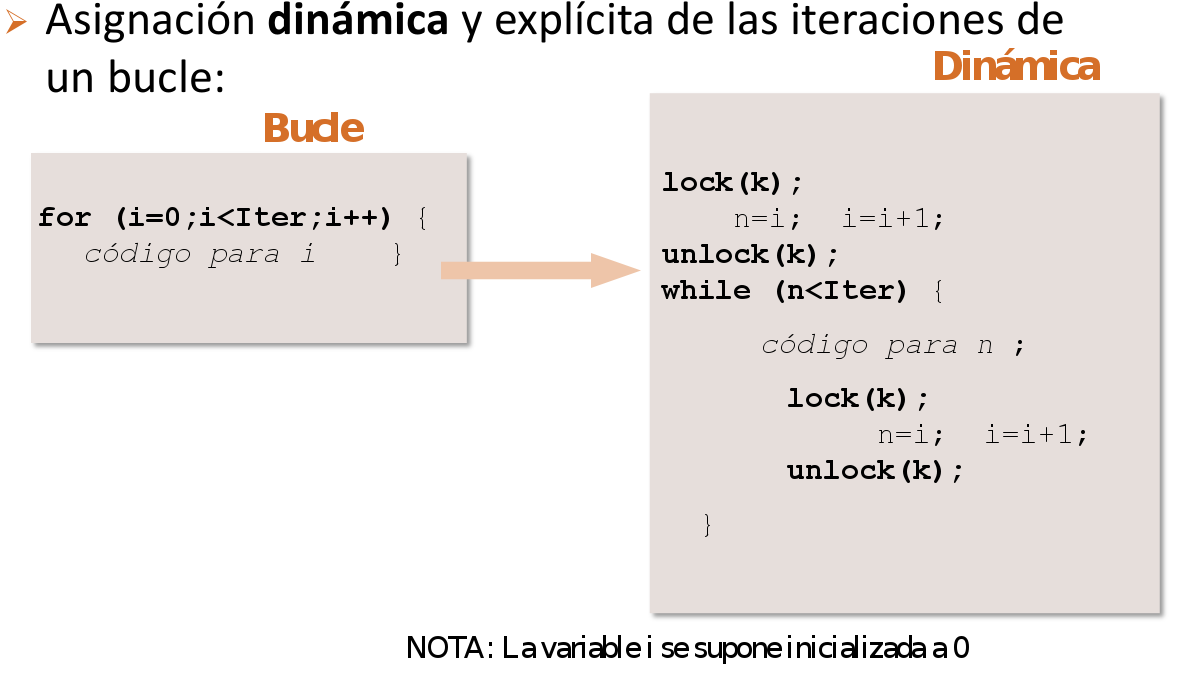
\includegraphics[width=0.7\textwidth]{44}
\caption{Asignación dinámica explícita de las tareas de un bucle a procesos/hebras}
\label{tipos_din_asig}
\end{figure}

La \hyperref[tipos_din_asig]{Figura \ref*{tipos_din_asig}} muestra cómo el programador puede implementar explícitamente en el código una asignación dinámica para memoria compartida. Las iteraciones se reparten en orden: primero la $0$, después la $1$, y así sucesivamente hasta la última. El índice $i$ del bucle es una variable compartida que consultan los procesos para ``coger'' la siguiente iteración que van a realizar e incrementan su valor en uno para que el siguiente proceso no coja una iteración ya asignada. Esto debe hacerse en exclusión mutua, para ello se usa un cerrojo $k$. Con paso de mensajes la asignación dinámica la haría el proceso dueño en un esquema dueño-esclavo.

Usando asignación dinámica añado tiempo de ejecución aunque la asignación de tareas es más equilibrada.

\textcolor[rgb]{0.2,0.4,0.8}{\subsubsection{Asignación de tareas a dos threads estáticas por round-robin para el cálculo de $\pi$}}
Si tenemos dos cores en nuestra máquina, podemos dividir el trabajo de cálcular áreas de rectángulos como se ve en la \hyperref[calculo_pi]{Figura \ref*{calculo_pi}}:

\begin{figure}[!h]
\centering
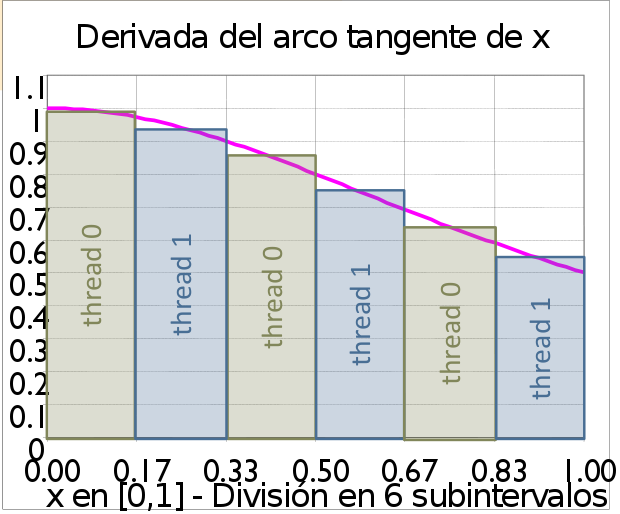
\includegraphics[width=0.3\textwidth]{47}
\caption{Cálculo de $\pi$ diviendo el área bajo la gráfica en 6 rectángulos}
\label{calculo_pi}
\end{figure}

Así, cada core calculará tres áreas y luego se sumarán los resultados de cada área para saber el valor de pi.

\textcolor[rgb]{0.2,0.4,0.8}{\subsubsection{Ejemplo: multiplicación matriz por vector}}
\begin{figure}[!h]
    \centering
    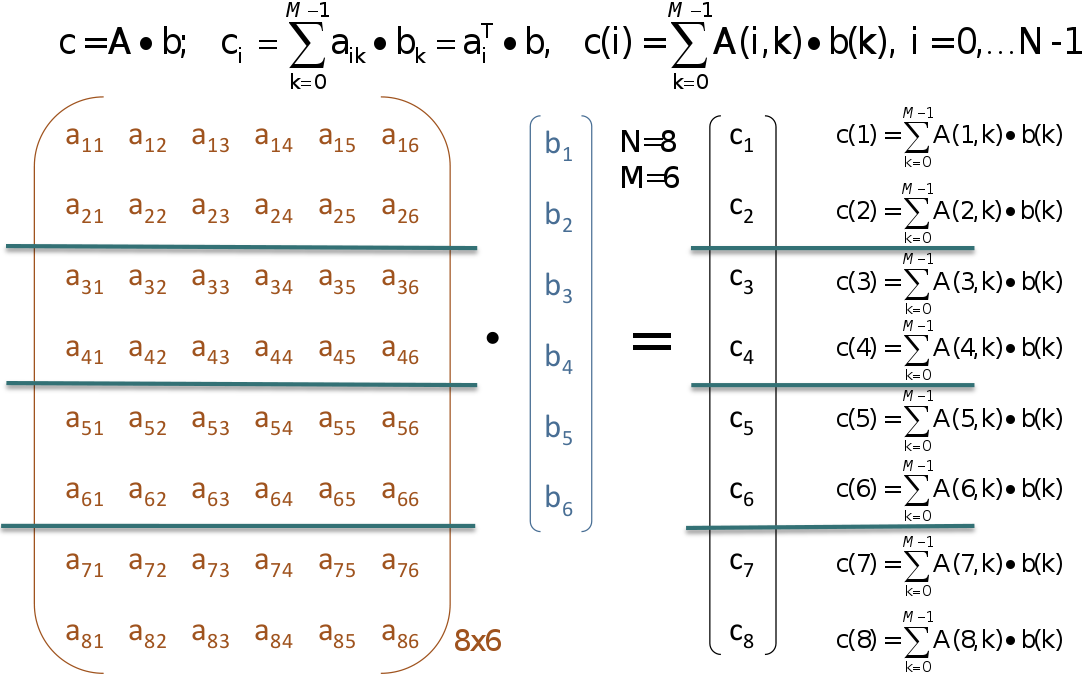
\includegraphics[width=0.7\textwidth]{45}
    \caption{Asignación por salida}
    \label{asig_filas}
\end{figure}

\begin{figure}[!h]
    \centering
    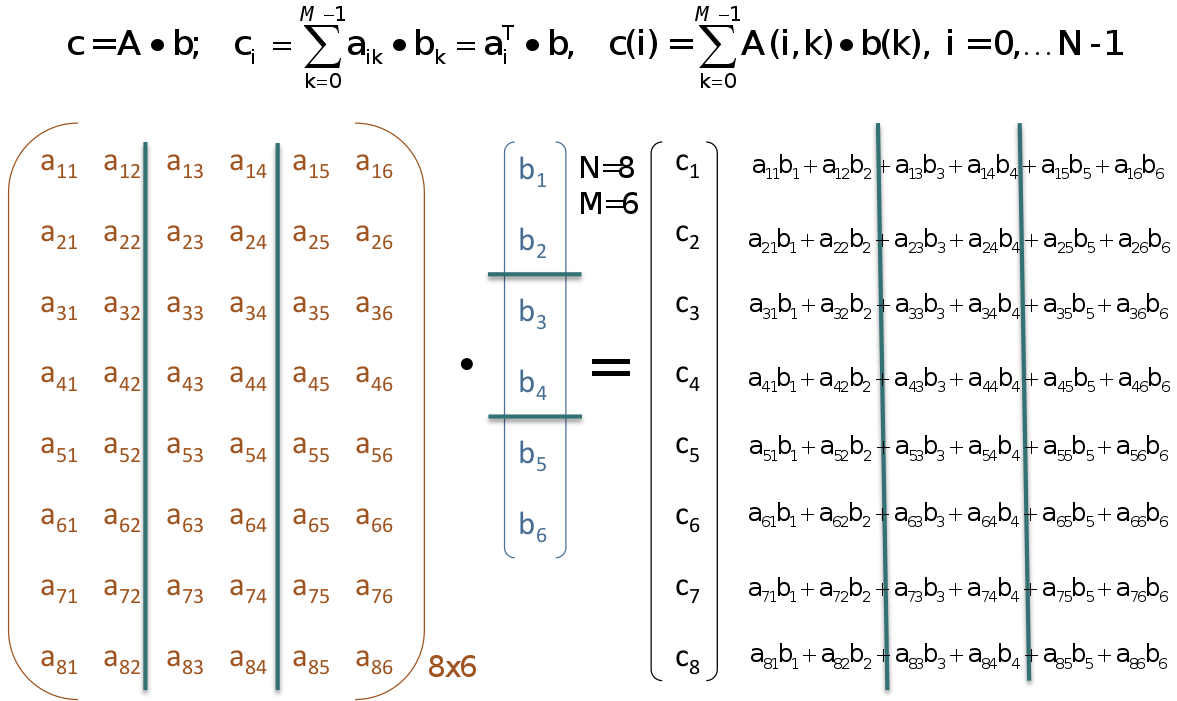
\includegraphics[width=0.7\textwidth]{46}
    \caption{Asignación por entradas}
    \label{asig_columnas}
\end{figure}

Para paralelizar un proceso que calcule la multiplicación de una matriz por un vector, podemos:
\begin{enumerate}[\color{azul}{\bf $\heartsuit$}]
    \item \textcolor[rgb]{0.2,0.4,0.8}{\textbf{Dividir las salidas de una tarea}}: (\hyperref[asig_filas]{Figura \ref*{asig_filas}}), así las operaciones para obtener $c(1)$ y $c(2)$, por ejemplo, las haría un thread y así. En esta alternativa no es necesaria comunicación entre los threads ya que cada uno calcula salidas definitivas
    \item \textcolor[rgb]{0.2,0.4,0.8}{\textbf{Dividir las entradas de una tarea}}: (\hyperref[asig_columnas]{Figura \ref*{asig_columnas}}), troceando la matriz por columnas (troceando las entradas también troceamos las salidas). En esta alternativa hay comunicación entre los threads ya que, por ejemplo, para calcular $c(1)$ tenemos cálculos en los tres threads. Esta alternativa es peor que la primera ya que en esta necesitamos comunicación y en la otra no.
\end{enumerate}

\textcolor[rgb]{0.2,0.4,0.8}{\subsection{Redactar código paralelo}}
El código paralelo va a depender de:
\begin{enumerate}[\color{azul}{\bf $\heartsuit$}]
    \item \textcolor[rgb]{0.2,0.4,0.8}{\textbf{Estilo de programación utilizado}}: variables compartidas, paso de mensajes, paralelismo de datos
    \item \textcolor[rgb]{0.2,0.4,0.8}{\textbf{Modo de programación}}: SPMD, MPMD mixto
    \item \textcolor[rgb]{0.2,0.4,0.8}{\textbf{Punto de partida}}: versión secuencial, descripción del problema
    \item \textcolor[rgb]{0.2,0.4,0.8}{\textbf{Herramienta software disponible para hacer explícito el paralelismo}}: lenguajes de programación, directivas, bibliotecas de funciones, compilador
    \item \textcolor[rgb]{0.2,0.4,0.8}{\textbf{Estructura}}: granja de tareas, segmentada, descomposición de datos, divide y vencerás, que depende a su vez de la aplicación.
\end{enumerate}

Habrá que añadir o utilizar en el programa las funciones, directivas o construcciones del lenguaje que hagan falta para:
\begin{enumerate}[\color{azul}{\bf $\heartsuit$}]
    \item \textcolor[rgb]{0.2,0.4,0.8}{\textit{Crear y terminar}} procesos, o en caso de que se creen de forma estática, \textcolor[rgb]{0.2,0.4,0.8}{\textit{enrolar}} y \textcolor[rgb]{0.2,0.4,0.8}{\textit{desenrolar}} procesos en el grupo que va a cooperar en el cálculo.
    \item \textcolor[rgb]{0.2,0.4,0.8}{\textit{Localizar}} el paralelismo
    \item \textcolor[rgb]{0.2,0.4,0.8}{\textit{Asignar}} la carga de trabajo conforme a la decisión tomada en el paso anterior
    \item \textcolor[rgb]{0.2,0.4,0.8}{\textit{\textcolor[rgb]{0.2,0.4,0.8}{Comunicar y sincronizar}}} los diferentes procesos/hebras.
\end{enumerate}

% \textcolor[rgb]{0.2,0.4,0.8}{\subsubsection{Cálculo de $\pi$ con OpenMP}}
% El código paralelo para el cálculo de $\pi$ con OpenMP y C es el siguiente:
% \begin{minted}[linenos]{c}
% #include <omp.h>
% #define NUM_THREADS 4
% int main (int argc, char **argv) {
%     long double ancho, x, sum=0; int intervalos, i;
%     intervalos = atoi(argv[1]);
%     ancho = 1.0/(double)intervalos;
%     omp_set_num_threads(NUM_THREADS);

%     // Crear/Terminar hebras
%     #pragma omp parallel
%     {
%         // Localizar
%         #pragma omp for /*Comunicar/sincronizar*/ reduction(+:sum) private(x) \
%                                 schedule(dynamic) /* Agrupar/asignar*/
%         for (i=0; i<intervalos; i++) {
%             x = (i+0.5)*ancho; sum=sum+4.0/(1.0+x*x);
%         }
%     }
%     sum *= ancho;
% }
% \end{minted}

\textcolor[rgb]{0.2,0.4,0.8}{\subsubsection{Cálculo de $\pi$ en MPI}}
El código para el cálculo de $\pi$ en MPI sería el siguiente:
\begin{minted}[linenos]{c}
#include <mpi.h>
int main (int argc, char **argv) {
    double ancho, x, lsum, sum; int intervalos, i, nproc, iproc;

    //Enrolar
    if (MPI_Init(&argc, &argv) != MPI_SUCCESS) exit(1);

    MPI_Comm_size(MPI_COMM_WORLD,&nproc);
    MPI_Comm_rank(MPI_COMM_WORLD,&iproc);

    intervalos=atoi(argv[1]);
    ancho=1.0/(double)intervalos; lsum=0;

    //Localizar/agrupar
    for (i=iproc; i<intervalos; i+=nproc) {
        x = (i+0.5)*ancho; lsum+=4.0/(1.0+x*x);
    }

    lsum*=ancho;

    //Comunicar/sincronizar
    MPI_Reduce(&lsum, &sum, 1, MPI_DOUBLE, MPI_SUM, 0, MPI_COMM_WORLD);

    //Desenrolar
    MPI_Finalize();
}
\end{minted}

A diferencia del código en OpenMP, en MPI al ser de un nivel de abstracción más bajo, tenemos que repartir las iteraciones del \verb*|for| y enrolar y desenrolar procesos manualmente.

\textcolor[rgb]{0.2,0.4,0.8}{\subsection{Evaluar prestaciones}}
Una vez redactado el código deben evaluarse sus prestaciones. Si no son las deseadas, debemos volver hacia atrás, se retrocederá más hacia atrás cuanto mayor sea la necesidad de mejora de prestaciones. 

Si se vuelve a la etapa de escritura puede elegirse otra herramienta de programación, ya que no todas ofrecen las mismas prestaciones. Se puede volver a la etapa de asignación para realizar un mejor reparto de la carga. Se puede volver a la etapa de descomposición para mejorar la descomposición en tareas o modificar el punto de partida.

\newpage
\textcolor[rgb]{0.2,0.4,0.8}{\section{Evaluación de prestaciones en procesamiento paralelo}}
\textcolor[rgb]{0.2,0.4,0.8}{\subsection{Ganancia en prestaciones y escabilidad}}
\textcolor[rgb]{0.2,0.4,0.8}{\subsubsection{Evaluación de prestaciones}}
Las medidas que se usan  para evaluar y comparar distintas realizaciones de una arquitectura son medidas genéricas, que se utilizan también en la evaluación de otros sistemas. En computadores paralelos suelen ser:
\begin{enumerate}[\color{azul}{\bf $\heartsuit$}]
    \item \textcolor[rgb]{0.2,0.4,0.8}{\textbf{Tiempo de ejecución (respuesta)}}: tiempo que supone la ejecución de una aplicación en el sistema. Puede ser el tiempo real (\textcolor[rgb]{0.2,0.4,0.8}{\textit{wall-clock time, elapsed time (/usr/bin/time)}}) ó el tiempo de usuario, sistema o la suma de ambos: el tiempo de CPU.
    \item \textcolor[rgb]{0.2,0.4,0.8}{\textbf{Productividad}}: número de aplicaciones que el computador es capaz de procesar por unidad de tiempo.
\end{enumerate}

Dependiendo de la utilización del sistema se le dará más énfasis a mejorar una u otra (se mejorará la productividad en, por ejemplo, una red de computadores y el tiempo de respuesta, en aplicaciones HPC), o en algunos casos se intentará mejorar ambos aspectos (por ejemplo: servidores de internet).

Además se utilizan otras medidas de prestaciones adicionales:
\begin{enumerate}[\color{azul}{\bf $\heartsuit$}]
    \item \textcolor[rgb]{0.2,0.4,0.8}{\textbf{Escabilidad}}: evolución de la ganancia en prestaciones que se consigue en el sistema conforme se añaden recursos. Pretende medir el nivel efectivo de aprovechamiento efectivo de los recursos. %Al comprador le interesa que su sistema pueda expandir sus prestaciones conforme aumenten sus necesidades y, por tanto, necesita saber hasta qué número de nodos se puede expandir el sistema y las prestaciones alcanzadas con cada ampliación.
    \item \textcolor[rgb]{0.2,0.4,0.8}{\textbf{Eficiencia}}: permite evaluar en qué medida las prestaciones que ofrece un sistema para un programa paralelo se acercan a las prestaciones máximas que idealmente debería ofrecer dado los recursos de los que dispone (por ejemplo, un programa secuencial que tarda en ejecutarse $T$, si hacemos una versión paralela y lo ejecutamos en un sistema con cuatro cores debería tardar $T/4$).

    Las prestaciones que se obtienen con $p$ recursos serían las prestaciones que se obtienen con un recurso multiplicado por $p$:
    \begin{displaymath}
    E(p,n) = \frac{Prestaciones(p,n)}{p\cdot Prestaciones(1,n)} = \frac{S(p,n)}{p}
    \end{displaymath}
    La ganancia máxima es $p$ por lo que la eficiencia máxima es $1$. Por otro lado, la ganancia mínima es $1$ por lo que la eficiencia mínima será $\frac{1}{p}$
\end{enumerate}

\textcolor[rgb]{0.2,0.4,0.8}{\subsubsection{Ganancia en prestaciones. Escalabilidad}}
Se utiliza la ganancia en velocidad para estudiar en qué medida se incrementan las prestaciones al ejecutar una aplicación en un sistema con múltiples procesadores frente a su ejecución en un sistema uniprocesador. Se puede obtener como:


\begin{displaymath}
S(p) = \frac{Prestaciones(p)}{Prestaciones(1)}
\end{displaymath}

Es decir, dividiendo las prestaciones que se consiguen en un sistema con $p$ procesadores entre las prestaciones conseguidas en una versión secuencial. Si usamos el tiempo de respuesta para evaluar las prestaciones, las prestaciones vendrían dadas por la inversa del tiempo:

\begin{displaymath}
S(p) = \frac{T_s}{T_p(p)} \qquad\ \textrm{con $T_p(p) = T_c(p) + T_o(p)$}
\end{displaymath}

Donde $T_s$ sería el tiempo de ejecución (respuesta) del programa secuencial y $T_p(p)$, el tiempo de ejecución del programa paralelo con $p$ procesadores. El tiempo de ejecución en paralelo depende del tiempo de cómputo $T_c(p)$ y del tiempo de penalización o sobrecarga (\textit{\textcolor[rgb]{0.2,0.4,0.8}{Overhead}}) $T_o(p)$ en el que influyen factores como:
\begin{enumerate}[\color{azul}{\bf $\heartsuit$}]
    \item Tiempo de comunicación/sincronización entre procesos
    \item Tiempo para crear/terminar (enrolar/desenrolar) los procesos
    \item Tiempo de ejecución de operaciones añadidas en la versión paralela no presentes en la secuencial.
\end{enumerate}

La penalización que supone la \textcolor[rgb]{0.2,0.4,0.8}{\textit{falta de equilibrado}} en la distribución de tareas está incluída en la sobrecarga si no se ha tenido en cuenta al determinar el tiempo de cómputo paralelo.

Tanto el tiempo de cálculo como el \textcolor[rgb]{0.2,0.4,0.8}{\textit{overhead}} dependen del número de procesadores. Cuanto mayor sea éste mayor será el \textcolor[rgb]{0.2,0.4,0.8}{\textit{grado de paralelismo}} de la aplicación aprovechado. El \textcolor[rgb]{0.2,0.4,0.8}{\textit{overhead}} depende del número de procesos involucrados ya que la comunicación/sincronización y el crear/terminar procesos dependen de éste número. 

\begin{figure}[!h]
\centering
\includegraphics[width=0.4\textwidth]{48}
\caption{Escalabilidad lineal, superlineal y sublineal}
\label{grafica_lineal}
\end{figure}

La representación de la ganancia en función del número de procesadores nos permite evaluar la escabilidad de una implementación paralela o de una arquitectura. Idealmente el tiempo se reduciría a $\frac{T_s}{p}$, pero para lograrlo, se debería poder distribuir el programa entre los procesadores y el \textcolor[rgb]{0.2,0.4,0.8}{\textit{overhead}} debería ser despreciable. En este caso, la ganancia sería $p$ y la escalabilidad sería \textcolor[rgb]{0.2,0.4,0.8}{\textit{lineal}} (\hyperref[grafica_lineal]{Figura \ref*{grafica_lineal}}). Para que la ganancia siempre pueda ser $p$, el \textcolor[rgb]{0.2,0.4,0.8}{\textit{grado de paralelismo}} debe ser ilimitado, es decir, siempre se podrá dividir el código entre los $p$ procesadores disponibles sea cual sea el valor de $p$ (\hyperref[modelos_secuencial]{Apartado $a)$ de la Figura \ref*{modelos_secuencial}}).

No obstante podemos encontrarnos a veces con una escalabilidad \textcolor[rgb]{0.2,0.4,0.8}{\textit{superlineal}} ($S(p) > p$), que se puede deber a que al aumentar el número de procesadores también aumentamos otros recursos (caché, memoria principal). Otra posibilidad es que estemos ejecutando una aplicación que consista en explorar un conjunto de posibilidades y en cuanto encuentre la posibilidad acertada termine. Por ejemplo, imaginemos que tenemos que explorar un vector de cuatro casillas donde la casilla tercera contiene la solución esperada:

\begin{center}
\input{ejemplo1.latex}
\end{center}

En una solución secuencial tardaríamos $3T$ en llegar a la solución correcta, en cambio, si hacemos una versión secuencial con dos threads dividiendo el trabajo de la siguiente manera:

\begin{center}
\input{ejemplo2.latex}
\end{center}

Sólo tardaríamos $T$ en encontrar la solución correcta, es decir, tres veces menos que con la versión secuencial.

\begin{figure}[!h]
\centering
\includegraphics[width=0.7\textwidth]{49}
\caption{Modelos de código secuencial}
\label{modelos_secuencial}
\end{figure}

Aunque hemos considerado que todas las tareas son paralelizables en la práctica siempre habrá una parte $f$ que no sea paralelizable y que supone un tiempo no despreciable.  Además, el grado de paralelismo, aunque lo hemos considerado ilimitado, estará limitado si se mantiene fijo el tiempo de ejecución secuencial $T_s$. Tampoco hemos considerado el tiempo de sobrecarga. 

\begin{tabular}{|p{2cm}|p{2cm}|p{2cm}|p{2cm}|p{7cm}|}
\hline
\rowcolor[rgb]{0.2,0.7,0.6} \textcolor[rgb]{1,1,1}{\textbf{Modelo código}} & \textcolor[rgb]{1,1,1}{\textbf{Fracción no paral. en $T_s$}} & \textcolor[rgb]{1,1,1}{\textbf{Grado paralelismo}} & \textcolor[rgb]{1,1,1}{\textbf{Overhead}} & \textcolor[rgb]{1,1,1}{\textbf{Ganancia en función del número de procesadores $p$ con $T_s$ constante}} \\
\hline
$a)$ & $0$ & ilimitado & $0$ & \begin{equation}S(p)=\frac{T_s}{T_p(p)} = p \quad\ \textrm{Ganancia Lineal} \label{primera} \end{equation} \\
\hline
$b)$ & $f$ & ilimitado & $0$ & \begin{equation}S(p) = \frac{1}{f+\frac{(1-f)}{p}} \quad\ p \rightarrow \infty \frac{1}{f} \label{segunda} \end{equation} \\
\hline
$c)$ & $f$ & $n$ & $0$ & \begin{equation}S(p) = \frac{1}{f+\frac{(1-f)}{p}} \quad\ p=n \quad\ \frac{1}{f+\frac{(1-f)}{n}} \label{tercera} \end{equation} \\
\hline
$b)$ & $f$ & ilimitado & incrementa linealmente con $p$ & \begin{equation}S(p) = \frac{1}{f+\frac{(1-f)}{p}+\frac{T_o(p)}{T_s}} \quad\ p \rightarrow \infty ~ 0 \label{cuarta} \end{equation} \\
\hline
\end{tabular}

En la tabla anterior se incluyen expresiones de ganancia en velocidad  para diferentes modelos de código secuencial. Las expresiones \ref*{primera}, \ref*{segunda}, \ref*{tercera} y \ref*{cuarta} se corresponden a las gráficas de la \hyperref[grafica_lineal]{Figura \ref*{grafica_lineal}}. 

En la expresión \ref*{tercera} se tiene en cuenta la presencia de código no paralelizable y que el grado de paralelismo puede ser menor que el número de procesadores disponibles ($n < p$), por tanto, la ganancia al incrementar el número de procesadores se limita cuando se aprovecha todo el grado de paralelismo de la aplicación.

En la expresión \ref*{cuarta} se tiene en cuenta la presencia de código no paralelizable y el tiempo de sobrecarga, que se incrementa linealmente con $p$. Se considera el grado de paralelismo ilimitado. Esta función presenta un máximo para $p$, es decir, llega un momento cuando incrementamos el número de procesadores que la ganancia deja de crecer y comienza a decrecer. Este decremento se inicia cuando al incrementar $p$ en $1$ se incrementa el término de la sobrecarga ($\frac{T_o(p)}{T_s}$) en mayor medida que se decrementa la parte del cálculo paralelo ($f + \frac{1-f}{p}$) de forma que el denominador de la expresión aumenta en lugar de disminuir.

\textcolor[rgb]{0.2,0.4,0.8}{\subsection{Ley de Amdahl}}
La ganancia en prestaciones utilizando $p$ procesadores está limitada por la fracción de código que no se puede paralelizar:
\begin{displaymath}
S(p) = \frac{T_s}{T_P(p)} \leq \frac{T_s}{f\cdot T_s + \frac{(1-f)\cdot T_s}{p}} = \frac{p}{1+f(p-1)} \rightarrow \frac{1}{f} (p \rightarrow \infty)
\end{displaymath}

Esta expresión se obtiene a partir de la expresión \hyperref[segunda]{\ref{segunda}}. Donde:
\begin{enumerate}[\color{azul}{\bf $\heartsuit$}]
    \item $S$ es el incremento en velocidad que se consigue al aplicar una mejora (paralelismo)
    \item $p$ es el incremento en velocidad máximo que se puede conseguir si se aplica la mejora todo el tiempo (número de procesadores)
    \item $f$ es la fracción de tiempo en el que no se puede aplicar la mejora (fracción de tiempo no paralelizable).
\end{enumerate}

\begin{figure}[!h]
\centering
\includegraphics[width=0.7\textwidth]{50}
\caption{Ganancia en prestaciones para varias fracciones de código no paralelizable}
\label{ley_de_a}
\end{figure}

La Ley de Amdahl nos da una visión pesimista de las ventajas de la paralelización, ya que nos dice que tenemos limitada la escalabilidad y que este límite depende de la fracción de código no paralelizable. En la \hyperref[ley_de_a]{Figura \ref*{ley_de_a}} se representa la ganancia en prestaciones (\hyperref[segunda]{expresión \ref*{segunda}}) en función de $p$ para diferentes fracciones de código no paralelizable. La escalabilidad decrece conforme se incrementa la fracción de código no paralelizable.

No obstante, se ha puesto constante el tiempo de ejecución secuencial $T_s$ y con ello, se ha considerado la fracción de ćodigo paralizable ($1-f$) constante también. Pero en muchas aplicaciones se puede aumentar la parte de código paralelizable aumentando el tamaño del problema.

Por ejemplo, en el modelo basado en un bucle (\hyperref[modelos_secuencial]{Apartado $c)$ de la Figura \ref*{modelos_secuencial}}). Probablemente el bucle opere con una estructura matricial. Incrementando su tamaño, incrementaremos el número de iteraciones y, por tanto, el grado de paralelismo y la fracción de código paralelizable.  En el ejemplo del cálculo de $\pi$, aumentar el tamaño del problema supone calcular $\pi$ con mayor precisión, ya que el error al calcular el área de los rectángulos (\hyperref[calculo_pi]{Figura \ref*{calculo_pi}}), disminuye el error (\hyperref[ganancia_pi]{Figura \ref*{ganancia_pi}})

\begin{figure}[!h]
\centering
\includegraphics[width=0.7\textwidth]{51}
\caption{Cálculo de $\pi$ con distintos tamaños del problema}
\label{ganancia_pi}
\end{figure}

\newpage
\textcolor[rgb]{0.2,0.4,0.8}{\subsection{Ganancia escalable}}
\textcolor[rgb]{0.2,0.4,0.8}{\subsubsection{Ley de Gustafson}}
\begin{figure}[!h]
\centering
\includegraphics[width=0.7\textwidth]{52}
\caption{Paralelización en $p$ procesadores con $n=kp$. Si $k$ es constante entonces el tiempo de ejecución en paralelo es constante ($T_p$)}
\label{ley_g}
\end{figure}

Supongamos un modelo de código secuencial con una parte no paralelizable, y un número de tareas a paralelizar $n$ que se puede incrementar aumentando el tamaño del problema (\hyperref[ley_g]{Figura \ref*{ley_g}}). Considerando despreciable el tiempo de \textcolor[rgb]{0.2,0.4,0.8}{\textit{overhead}}, podemos mantener constante el tiempo de ejecución en paralelo $T_p$ variando el número de procesadores $p$ y el tamaño $n$ de forma que $n=kp$ , con $k$ constante. Así, el tiempo de ejecución sólo depende del tiempo de ejecución secuencial $T_s(n)$. Así, la ganancia en prestaciones sería:

\begin{displaymath}
S(p) = \frac{T_s(n)}{T_p} = \frac{fT_p + p(1-f)T_p}{T_p} = \frac{f\cancel{T_p}+p(1-f)\cancel{T_p}}{\cancel{T_p}} = p(1-f) + f
\end{displaymath}

¡Ojo!, en este caso \textbf{$f$ es la fracción del programa NO PARALELIZABLE que corresponde a $T_p$}, mientras que en la ley de Amdahl la $f$ es la fracción del programa no paralelizable que corresponde a $T_s$, es muy importante no confundirlas y ver la diferencia clara. En la expresión lo único que varía es $p$.

La expresión viene del dibujo que tenemos en la \hyperref[ley_g]{Figura \ref*{ley_g}}, como se ve en la foto tenemos por un lado una fracción de programa no paralelizable ($fT_p$) y por otro lado tenemos $k$ conjuntos de $p$ bloques de código paralelo que se con la fracción $1-f$ ($p(1-f)T_p$).

La ganancia depende linealmente del número de procesadores $p$ con una pendiente $1-f$, que es la fracción de tiempo que supone la ejecución de la parte paralela. Cuanto mayor sea $1-f$ mayor será la escalabilidad.

\textcolor[rgb]{0.2,0.4,0.8}{\chapter{Arquitecturas con paralelismo de thread (TLP)}}
\setcounter{section}{6}
\textcolor[rgb]{0.2,0.4,0.8}{\section{Arquitecturas TLP}}
\textcolor[rgb]{0.2,0.4,0.8}{\subsection{Clasificación de arquitecturas con TLP explícito y una instancia del sistema operativo}}
\begin{enumerate}[\color{azul}{\bf $\heartsuit$}]
    \item \textbf{\textcolor[rgb]{0.2,0.4,0.8}{Multicomputador}}: puede ejecutar múltiples flujos de control en paralelo, cada flujo de control se ejecuta en un core distinto. Se puede ver empaquetado en diferentes niveles de encapsulación:
    \begin{enumerate}[$\longrightarrow$]
        \item a nivel de chip (multicores)
        \item a nivel de placa
        \item a nivel de sistema (un sistema está compuesto de armarios)
    \end{enumerate}
    \item \textcolor[rgb]{0.2,0.4,0.8}{\textbf{Multicore o multiprocesador en un chip o CMP (\textit{Chip MultiProcessor})}}: es un multiprocesador en un chip, es decir, ejecuta varios threads en paralelo en un chip de procesamiento multicore (cada thread en un core distinto)
    \item \textcolor[rgb]{0.2,0.4,0.8}{\textbf{Core multithread}}: Se puede modificar la arquitectura superescalar y segmentada de un core para que pueda ejecutar múltiples flujos de control concurrentemente o incluso, en paralelo (\textcolor[rgb]{0.2,0.4,0.8}{\textit{Hyperthreading}}). %DUDA: en la sincronización de dos cores lógicos que forman parte de uno mismo físico hay paso de mensajes?
\end{enumerate}

\textcolor[rgb]{0.2,0.4,0.8}{\subsection{Multiprocesadores}}
\textcolor[rgb]{0.2,0.4,0.8}{\subsubsection{Criterio de clasificación: sistema de memoria}}
Esta clasificación la vimos en el \hyperref[clasif_memoria]{Tema 1}.
\begin{enumerate}[\color{azul}{\bf $\heartsuit$}]
    \item \textcolor[rgb]{0.2,0.4,0.8}{\textbf{Multiprocesador con memoria centralizada (UMA)}}: el acceso a memoria en los procesadores tarda el mismo tiempo independientemente de la dirección de memoria a la que se acceda y desde el procesador desde el que se acceda, esto quiere decir que todos los procesadores se encuentran a la misma distancia de las direcciones de memoria. Se accede a memoria a través de una red de interconexión que puede ser un bus, una multietapa o barras cruzadas.

    Esta alternativa presenta una mayor latencia por el hecho de que todos los procesadores acceden a la memoria de manera compartida, por tanto, es bastante probable que haya colisiones (dos procesadores quieren acceder a la misma posición de memoria). También presentan poca escalabilidad puesto que cuanto mayor sea el número de procesadores mayor será el número de colisiones en el acceso a memoria.

    \item \textcolor[rgb]{0.2,0.4,0.8}{\textbf{Multiprocesador con memoria distribuida (NUMA)}}: el acceso a memoria no es uniforme porque la memoria está distribuida entre los nodos de procesamiento. Cada uno de los procesadores tiene cerca un módulo de memoria, por tanto puede acceder a las direcciones de memoria que tiene cerca más rápido que las direcciones de memoria que tiene lejos. Esta alternativa es más escalable, puede llegar a cientos/miles de cores porque cada procesador accede normalmente a las posiciones de memoria que tiene más cerca suyo y por tanto, el número de colisiones es muy pequeño. Los diferentes tipos de red de interconexión para acceder a la memoria de los demás procesadores suelen ser barras cruzadas, multietapa, árbol grueso y anillo.
\end{enumerate}

\textcolor[rgb]{0.2,0.4,0.8}{\subsubsection{Criterio de clasificación: nivel de empaquetamiento/conexión}}
Como dijimos antes, los multiprocesadores pueden venir presentados de diferentes formas:

\begin{center}
\input{emp.latex}
\end{center}

Cada una de las diferentes formas está formada por la forma anterior, así, por ejemplo, un sistema será un conjunto de armarios, un armario será un conjunto de placas y una placa será un conjunto de chips.

\textcolor[rgb]{0.2,0.4,0.8}{\subsubsection{Evolución de multiprocesadores en una placa}}
Han evolucionado de UMA a NUMA. 

En un UMA, la comunicación de la CPU con la memoria se hacía a través de un bus y el chipset (conjunto de chips que se usa para la conexión de la CPU con elementos externos: suele estar formado por dos chips, el \textit{\textcolor[rgb]{0.2,0.4,0.8}{puente norte}}, que conecta cpu con memoria y graficos, y el \textit{\textcolor[rgb]{0.2,0.4,0.8}{puente sur}}, que conecta CPU con dispositivos lentos).

Ahora lo que se suele ver más son estructuras NUMA: los chips de procesamiento están conectados directamente a la memoria. Ya no tenemos buses, sino conmutadores y enlaces. La interfaz de red está incluida en los chips junto a los cores. El puente norte ahora sólo está para la conexión con los gráficos. Aunque hay PCs que tienen directamente los gráficos conectados, en ese caso no habría puente norte y el chipset estaría formado por uno sólo, el puente sur.


La estructura de un \textcolor[rgb]{0.2,0.4,0.8}{\textit{Intel Xeon 7300}} (\hyperref[intel_7300]{Figura \ref*{intel_7300}}) es una estructura intermedia entre las dos con un bus para cada CPU. Se corresponde con una placa de tipo UMA.

\begin{figure}[!h]
\centering
\includegraphics[width=0.3\textwidth]{53}
\caption{Estructura de un Intel Xeon 7300}
\label{intel_7300}
\end{figure}

Y en la \hyperref[intel_7500]{Figura \ref*{intel_7500}} nos encontramos una estructura más actual, de tipo NUMA. La red de interconexión que se usa para conectar los chips de procesamiento conecta los módulos de memoria de cada procesador dos a dos.

\begin{figure}[!h]
\centering
\includegraphics[width=0.7\textwidth]{54}
\caption{Estructura de un Intel Xeon 7500}
\label{intel_7500}
\end{figure}

\textcolor[rgb]{0.2,0.4,0.8}{\subsection{Multicores}}
% Los cores comparten el último nivel de caché. El controlador de la memoria ya no está en el puente norte sino en la memoria. Los cores de un mismo chip se pueden comunicar a través de la caché L3, si no comparten la caché, no se pueden comunicar procesadores porque no comparten la caché.

% En otras alternativas el comutador está en medio, se usa para acceder a la caché compartida.

Hay varias variantes para el diseño de multicores, que difieren en el número de cores, la estructura y tamaño de las cachés, el acceso de los cores a las cachés y la heterogeneidad de sus componentes.

Una posible estructura sería una en la que todos los cores compartieran al menos el último nivel de caché (\hyperref[je]{Figura \ref*{je}}). Así, los cores pueden comunicarse con ellos a través de este último nivel de caché sin acceder a memoria principal.

\begin{figure}[!h]
\centering
\includegraphics[width=0.7\textwidth]{55}
\caption{Estructura en forma de jerarquía}
\label{je}
\end{figure}

Otras posibles estructuras (\hyperref[as]{Figura \ref*{as}}) pueden ser, por ejemplo, hacer que la mitad de los procesadores compartan su último nivel de caché y la otra mitad comparta un último nivel de caché diferente (\hyperref[a1]{Figura \ref*{a1}}). En este caso, para implementar la comunicación entre cores tendremos que procurar que se comuniquen aquellos que compartan el último nivel de caché.

\begin{figure}[!h]
\centering
\mbox {
\subfigure[Alternativa 1: compartir el último nivel  de caché entre unos pocos procesadores]{
\label{a1}
\includegraphics[width=0.4\textwidth]{56}
}
\qquad
\subfigure[Alternativa 2: no compartir el último nivel de caché] {
\label{a2}
\includegraphics[width=0.4\textwidth]{57}
}
}
\subfigure[Alternativa 3: poner un conmutador entre los cores y el último nivel de caché]{
\label{a3}
\includegraphics[width=0.4\textwidth]{58}
}
\caption{Alternativas de estructuración de un multicore}
\label{as}
\end{figure}

O directamente, no compartir ningún nivel de caché entre cores, para lo cual tendremos que acceder a memoria principal si queremos comunicarlos (\hyperref[a2]{Figura \ref*{a2}}).

También podríamos poner un conmutador en entre los cores y el último nivel de caché compartido para regular el acceso al último nivel de caché (\hyperref[a3]{Figura \ref*{a3}})

\textcolor[rgb]{0.2,0.4,0.8}{\subsection{Cores Multithread}}
\textcolor[rgb]{0.2,0.4,0.8}{\subsubsection{Arquitecturas ILP}}
La arquitectura ILP puede ser de tres tipos: segmentada, VLIW y superescalar. 

En un procesador segmentado se insertan registros para crear un cauce. En un RISC es típico un cauce de cinco etapas:
\begin{enumerate}[\color{azul}{\bf $\heartsuit$}]
    \item \textbf{\textcolor[rgb]{0.2,0.4,0.8}{IF (\textit{Instruction Fetch})}}: etapa de captación de instrucciones. De la caché de instrucciones se coge la siguiente instrucción a ejecutar y se guarda en un registro intermedio (\textit{\textcolor[rgb]{0.2,0.4,0.8}{Instruction Buffer}}).
    \item \textbf{\textcolor[rgb]{0.2,0.4,0.8}{ID (\textit{Instruction Decode})}}: etapa de decodificación de instrucciones y emisión a unidades funcionales. Se decodifica la instrucción y se guarda en un registro intermedio.
    \item \textcolor[rgb]{0.2,0.4,0.8}{\textbf{EX (\textit{Execution})}}: etapa de ejecución. Se ejecuta la instrucción y se guardan los resultados en un registro intermedio.
    \item \textcolor[rgb]{0.2,0.4,0.8}{\textbf{MEM (\textit{Memory})}}: etapa de acceso a memoria. Se recogen los resultados de dicho registro intermedio y se guardan en memoria.
    \item \textcolor[rgb]{0.2,0.4,0.8}{\textbf{WB (\textit{Write-Back})}}: etapa de almacenamiento de resultados. Se modifican los registros de la arquitectura (tales como \verb*|rax|).
\end{enumerate}

\begin{figure}[!h]
\centering
\includegraphics[width=0.7\textwidth]{59}
\caption{Arquitectura escalar segmentada}
\label{arq_es}
\end{figure}

Un procesador segmentado permite ejecutar instrucciones concurrentemente, en la \hyperref[arq_es]{Figura \ref*{arq_es}} 5 instrucciones concurrentes cada una en una etapa del cauce. Es concurrente porque todas comparten el mismo hardware.

% En las otras dos alternativas, podemos tener instrucciones ejecutándose a la vez ya que hay varias unidades de funcionales y emiten múltiples instrucciones en paralelo a unidades funcionales. 

En las otras dos alternativas podemos tener instrucciones ejecutándose a la vez porque la unidad disponde de varias unidades funcionales a las que se les pueden emitir múltiples instrucciones en paralelo a las distintas unidades funcionales

Hay una unidad para punto fijo, otra para punto flotante, otra para cargar y guardar datos, etc. La unidad de punto flotante suele estar segmentada al igual que la unidad de memoria (calcular la dirección y acceder). Para decir que un core es superescalar, debe emitir varias instrucciones en el mismo ciclo de reloj a cada una de las unidades de ejecución. 

Las diferencias entre VLIW y superescalar son:
\begin{enumerate}[\color{azul}{\bf $\heartsuit$}]
    \item \textbf{\textcolor[rgb]{0.2,0.4,0.8}{VLIW}}:
    \begin{enumerate}[$\longrightarrow$]
        \item Las instrucciones que se ejecutan en paralelo se captan juntas de memoria
        \item Este conjunto de instrucciones conforman la palabra de instrucción muy larga a la que hace referencia la denominación VLIW
        \item El hardware presupone que las instrucciones de una palabra son independientes: no tiene que encontrar instrucciones que pueden emitirse y ejecutarse en paralelo.
    \end{enumerate}
    \item \textbf{\textcolor[rgb]{0.2,0.4,0.8}{Superescalares}}:
    \begin{enumerate}[$\longrightarrow$]
        \item Tiene que encontrar instrucciones que puedan emitirse y ejecutarse en paralelo (tiene hardware para extraer paralelismo a nivel de instrucción).
    \end{enumerate}
\end{enumerate}

Es decir, las instrucciones en VLIW se captan juntas en la memoria, porque no hay hardware para evitar problemas (WAW, WAR, RAW). Los superescalares, tienen hardware para eliminar problemas de paralelismo.

Son segmentados también: ejecutan instrucciones concurrentemente y en paralelo. 

\begin{figure}[!h]
\centering
\includegraphics[width=0.7\textwidth]{60}
\caption{Arquitecturas VLIW y superescalar}
\label{arq_vs}
\end{figure}

\textcolor[rgb]{0.2,0.4,0.8}{\subsection{Modificación de la arquitectura ILP en Core Multithread}}
Las modificciones hardware permiten a los threads multiplexar (unas veces en un ciclo de reloj lo usa un thread y en otro ciclo de reloj otro) el uso del hardware, repartir o compartir (dinámicamente se va asignando los recursos a cada thread en función de sus necesidades, con la alternativa de repartir, si un thread tiene asignado dos recursos pero sólo usa uno, el recurso que no usa no puede ser usado por otro thread.) entre cada thread, por último, se puede replicar un recurso (en los cores multithread se suele replicar el fichero de registro de la arquitectura: uno por thread).

\begin{figure}[!h]
\centering
\includegraphics[width=0.7\textwidth]{61}
\caption{Modificación de la arquitectura ILP en un core multithread}
\label{mod_arq}
\end{figure}

Por ejemplo, en la \hyperref[mod_arq]{Figura \ref*{mod_arq}}, se han repartido las cachés (tanto de datos como de instrucciones) y se ha replicado el fichero de registro, uno para cada thead.

\textcolor[rgb]{0.2,0.4,0.8}{\subsection{Clasificación de cores multithread}}
\begin{enumerate}[\color{azul}{\bf $\heartsuit$}]
    \item \textcolor[rgb]{0.2,0.4,0.8}{\textbf{Multihread temporal}}: se ejecutan concurrentemente, deben hacer un uso mayor de multiplexación. Aquí hay conmutación entre threads porque en un ciclo de reloj no hay varios threads ejecutándose a la vez. La conmutación la controla el hardware, no el sistema operativo. Hay varios tipos:
    \begin{enumerate}[$\longrightarrow$]
        \item \textcolor[rgb]{0.2,0.4,0.8}{\textbf{Grano fino}}: cada ciclo de reloj se cambia de thread, la conmutación se puede hacer con turnos rotatorios (no hay decisión sobre a qué thread se va a comutar) con un hardware muy sencillo (no tiene hardware para eliminar dependencias de datos, el número de etapas se fija para que no haya dependencias de WAR y WAW. Si tenemos menos threads de los predeterminados perdemos ciclos de reloj). También se puede conmutar a otros threads por eventos\footnote{dependencia funcional, acceso a datos a cache L1, salto no predecible, operación con cierta latencia} de latencia combinado con alguna técnica de planificación
        \item \textbf{\textcolor[rgb]{0.2,0.4,0.8}{Grano grueso}}: se conmuta entre threads pero no cada ciclo de reloj, la conmutación entre threads la decide el hardware tras intervalos de tiempo prefijados (\textcolor[rgb]{0.2,0.4,0.8}{\textit{timeslice multithreading}}) ó por eventos de cierta latencia (\textcolor[rgb]{0.2,0.4,0.8}{\textit{switch-on-event multithreading}}). Los granos gruesos a su vez se clasifican según su conmutación por eventos:
        \begin{itemize}
            \item \textcolor[rgb]{0.2,0.4,0.8}{\textbf{Estática}}: la conmutación puede hacerse \textit{\textcolor[rgb]{0.2,0.4,0.8}{explícita}} (instrucciones explícitas para la conmutación, el programador o el compilador pueden definir de forma explícita cuando cambiar de contexto) ó \textcolor[rgb]{0.2,0.4,0.8}{\textit{implícita}} con instrucciones de carga, almacenamiento o salto. El coste del cambio de contexto es bajo, pero se hacen cambios de contexto innecesarios.
            \item \textcolor[rgb]{0.2,0.4,0.8}{\textbf{Dinámica}}: la conmutación se hace cuando es necesario por un fallo en la última caché dentro del chip de procesamiento (conmutación por fallo de cache), interrupción (conmutación por señal),... Reduce cambios de contexto innecesarios pero tiene una mayor sobrecarga al cambiar de contexto. En este caso, los cambios de contexto son acciones propias de la instrucción.
        \end{itemize}
    \end{enumerate}
    \begin{figure}[!h]
    \centering
    \includegraphics[width=0.1\textwidth]{62}
    \caption{Esquema de dos threads ejecutándose en un multithread temporal}
    \label{mul_t}
    \end{figure}
    La \hyperref[mul_t]{Figura \ref*{mul_t}} refleja la ejecución de dos threads en un multithread temporal: ambos se van conmutando según indique el hardware. En el caso de B, deja sin usar un recurso durante tres ciclos de reloj pues no lo necesita.

    \item \textcolor[rgb]{0.2,0.4,0.8}{\textbf{Simultaneo}}: se ejecutan, en un core superescalar, varios threads en paralelo y comparten la unidad de ejecución. Pueden emitir (para su ejecución) instrucciones de varios threads en un ciclo.

    \begin{figure}[!h]
    \centering
    \includegraphics[width=0.1\textwidth]{63}
    \caption{Esquema de dos threads ejecutándose en un multithread simultáneo}
    \label{mul_s}
    \end{figure} 

    La \hyperref[mul_s]{Figura \ref*{mul_s}} muestra el esquema de dos threads ejecutándose en un thread simultáneo: ambos se van ejecutando paralelamente y así conseguimos un mayor aprovechamiento de los recursos.
\end{enumerate}

El objetivo de los cores multithreads es que las pérdidas de tiempo debido a accesos a memoria, dependencias RAW, etc. no sean visibles durante la ejecución de la instrucción, sino que si un thread falla o tiene que acceder a memoria, pueda seguir la ejecución otro thread, ya sea de forma concurrente o paralela, para evitar pérdidas de ciclos de reloj por esperar para poder seguir con la ejecución. Estos ciclos se evitan ejecutando instrucciones de threads distintos.

\begin{figure}[!h]
\centering
\includegraphics[width=0.7\textwidth]{65}
\caption{Alternativas en un core escalar segmentado}
\label{alt_multit}
\end{figure}

En un thread se pueden producir:
\begin{enumerate}[\color{azul}{\bf $\heartsuit$}]
    \item \textcolor[rgb]{0.2,0.4,0.8}{\textit{Pérdidas verticales}}: eliminables con threads de grano grueso y fino
    \item \textcolor[rgb]{0.2,0.4,0.8}{\textit{Pérdidas horizontales}}: no eliminables porque no se pueden ejecutar a la vez instrucciones de threads diferentes. Se pueden evitar con threads simultáneos gracias al multithread, ya que en el mismo ciclo se pueden ejecutar instruciones de threads distintos.
\end{enumerate}

\begin{figure}[!h]
\centering
\includegraphics[width=0.7\textwidth]{64}
\caption{Alternativas en un core con emisión múltiple de instrucciones de un thread}
\label{alt_multit}
\end{figure}

En la \hyperref[cuatro_vs_dos]{Figura \ref*{cuatro_vs_dos}} podemos ver una ejecución de cuatro procesos en un core de cuatro threads y la misma ejecución en dos cores con dos threads. ¿Si las dos pueden ejecutar cuatro threads en paralelo, cuál de las dos es más ventajosa?

En la opción de la izquierda, para que haya 4 threads simultáneos, necesitan darse cuatro instrucciones diferentes para ejecutar (es decir, que se necesite usar el registro de punto fijo, punto flotante, de salto y acceso a memoria), lo que puede dar lugar a pérdidas horizontales. Sin embargo, en la segunda opción, ejecutar todos los threads es más fácil porque sólo tenemos que tener en cuenta dos instrucciones por core al haber sólo dos threads por core.

Respecto a la replicación, algunos diseños de grano grueso sólo replican el contador de programa, pero en la mayoría de los casos, se replica todo, es decir, los registros.

\begin{figure}[!h]
\centering
\includegraphics[width=0.7\textwidth]{66}
\caption{Core multithread simultánea y multicores}
\label{cuatro_vs_dos}
\end{figure}

\textcolor[rgb]{0.2,0.4,0.8}{\section{Coherencia del sistema de memoria}}

En los CC-NUMA, los UMA y los COMA se implementa coherencia por hardware

\textcolor[rgb]{0.2,0.4,0.8}{\subsection{Sistema de memoria en multiprocesadores}}
El sistema de memoria incluye las caches de todos los nodos, la memoria principal, los buffers (tanto de escritura/almacenamiento como los buffer que combinan escrituras/almacenamientos) y la red de interconexión para acceder desde un procesador a los módulos de memoria directamente conectados a él y para acceder a direcciones remotas, conectadas a otro procesador. En resumen, el sistema de memoria incluye todo lo resaltado en rojo de la figura \hyperref[sis_mem]{Figura \ref*{sis_mem}}.

Dentro del chip de procesador está incluido el conmutador, los niveles de cache y los buffers.

\begin{figure}[!h]
\centering
\includegraphics[width=0.7\textwidth]{67}
\caption{Sistema de memoria}
\label{sis_mem}
\end{figure}

La comunicación de datos entre procesadores la realiza el sistema de memoria. La lectura de una dirección debe devolver lo último que se ha escrito, desde el punto de vista de todos los componentes del sistema.

\textcolor[rgb]{0.2,0.4,0.8}{\subsection{Concepto de incoherencia}}
La utilización de jerarquía de memoria, con el fin de acercar la velocidad de acceso a memoria a la velocidad del procesador, posibilita que pueda haber varias copias de un mismo bloque de memoria. Si dichas copias no tienen el mismo contenido, tendremos una \textcolor[rgb]{0.2,0.4,0.8}{\textit{incoherencia en el sistema de memoria}}.

Se pueden dar situaciones de incoherencia entre la memoria principal y las caches, o entre las distintas caches:

\begin{tabular}{|p{5cm}|p{6.5cm}|p{3.5cm}|}
\hline
\textbf{Clases de estructuras de datos} & \textbf{Causa de problemas por falta de coherencia} & \textbf{Falta de coherencia} \\
\hline
Datos modificables & E/S & Cache$-$MP \\
\hline
Datos modificables compartidos & Fallo de cache & Cache$-$MP \\
\hline
Datos modificables privados & Emigra proceso$\rightarrow$Fallo de cache & Cache$-$MP \\
\hline
Datos modificables compartidos & Lectura de cache no actualizada & Cache$-$Cache\\
\hline
\end{tabular}

En el ejemplo de la \hyperref[ejemplo_coherencia]{Figura \ref*{ejemplo_coherencia}}, el procesador $P_k$ lee de la posición de memoria $D$ ($1L$), lo que provoca que el bloque de memoria donde se encuentra esta dirección se copie a su cache. Tras la transferencia, el contenido de la posición de memoria $D$ en la cache es $3$, coincide con el contenido de la dirección en memoria principal. Si a continuación $P_k$ escribe un nuevo valor, $4$, en la dirección $D$ ($2E$), escribirá en la copia que tiene en su cache y dará lugar a una incoherencia en el sistema de memoria, ya que la posición $D$ no tiene el mismo contenido en memoria principal y en la caché.

\begin{figure}[!h]
\centering
\includegraphics[width=0.4\textwidth]{68}
\caption{Incoherencia entre memoria principal y cache. L denota lectura y E escritura. Mediante un número se indica el orden entre operaciones}
\label{ejemplo_coherencia}
\end{figure}

La memoria principal se suele dividir en bloques, que suelen ser de 64 bytes. Las caches también están divididas en bloques del mismo tamaño, llamados marcos de bloque. La unidad de acceso a memoria es un bloque. Si transferimos el bloque tenemos mayor velocidad de transferencia que transfiriendo palabras.

\textcolor[rgb]{0.2,0.4,0.8}{\subsubsection{Métodos de actualización de memoria principal implementados en caches}}
Para resolver las incoherencias entre memoria principal y caches hay dos métodos:
\begin{enumerate}[\color{azul}{\bf $\heartsuit$}]
    \item \textbf{\textcolor[rgb]{0.2,0.4,0.8}{Escritura inmediata}}: nunca habrá incoherencia porque al escribir en un bloque de cache se escribe en memoria principal. Cada escritura supone la utilización de la red y supone además un desaprovechamiento del ancho de banda de la red al transferir sólo datos aislados. Además, cuando se escribe en una dirección de memoria, suele escribirse varias veces en dicha dirección o en direcciones cercanas, por tanto, si la cache implementa esta alternativa tendríamos que hacer 64 transferencias a través de la red. Sería más deseable transferir todo el bloque de una vez.

    \item \textbf{\textcolor[rgb]{0.2,0.4,0.8}{Posescritura}}: se actualiza la memoria principal cuando se reemplaza el bloque en cache. Cuando se va a traer un bloque desde memoria principal y no queda espacio en cache, se reemplaza uno de los bloques que hay en cache. Si el bloque a reemplazar ha sido modificado (su ``bit sucio'' está activo), se escribe en memoria principal. Reduce comunicaciones pero permite que haya incoherencia, eso sí, con un sistema hardware que devuelve los valores actualizados de dicha posición de memoria. Para saber que un bloque ha sido modificado en la cache, se guarda en una tabla qué bloques de memoria principal están en cache y, para cada bloque, se guarda información sobre su estado, más concretamente si se ha modificado o no (\textcolor[rgb]{0.2,0.4,0.8}{\textit{bit sucio}})
\end{enumerate}

\newpage
\textcolor[rgb]{0.2,0.4,0.8}{\subsubsection{Alternativas para propagar una escritura en protocolos de coherencia de cache}}
En las caches no se admite incoherencia. Siempre se propaga lo que se escribe en una cache al resto. Para realizar dicha propagación tenemos dos alternativas:
\begin{enumerate}[\color{azul}{\bf $\heartsuit$}]
    \item \textcolor[rgb]{0.2,0.4,0.8}{\textbf{Escritura con actualización}}: siempre que se modifica una dirección en la copia de un bloque en la cache de un procesador, se modifica la dirección en todas las copias del bloque que se encuentren en todas las caches de otro procesadores.
    \item \textcolor[rgb]{0.2,0.4,0.8}{\textbf{Escritura con invalidación}}: cuando se va a modificar una dirección en la cache de un procesador, primero se invalidan las copias del bloque que contiene esa dirección en otras caches. Así, el procesador que va a modificar la dirección obtiene acceso exclusivo al bloque que la contiene. Cuando otra cache quiera leer ese dato tendrá que acceder a memoria principal obteniendo así una copia actualizada. Invalidar es más rápido que actualizar porque al invalidar sólo transferimos la dirección en la que se va a escribir mientras que al actualizar se deben transferir también los datos. Además, la invalidación permite compartir un bloque de memoria mientras se lee del bloque. También se reduce el número de transferencias puesto que si el bloque vuelve a modificar la dirección no originará transferencias. Sin embargo, si se va a actualizar un dato para que lo lean los demás procesadores puede ser más eficiente la actualización.
\end{enumerate}

\textcolor[rgb]{0.2,0.4,0.8}{\subsubsection{Situación de incoherencia aunque se propagan las escrituras (se usa difusión)}}
La propagación sólo sirve si usamos buses, pues no pueden hacerse accesos a memoria en paralelo. Sin embargo, hoy en día apenas se usan buses. Por ello, aun usando difusión podemos llegar a una situación de incoherencia.

Por ejemplo, el procesador de la \hyperref[sis_mem]{Figura \ref*{sis_mem}} tiene una variable $A$ con valor inicial $0$ y todas las caches tienen una copia de dicha variable.

\begin{figure}[!h]
\centering
\includegraphics[width=0.5\textwidth]{69}
\caption{Situación de incoherencia usando difusión}
\label{incoherencia_caches}
\end{figure}

Como el tiempo de transferencia depende de la longitud del enlace, el tiempo de transferencia entre $P0$ y $P2$ será mayor que entre $P0$ y $P1$.

$P0$ escribe en $A$ un $1$ y después, $P1$ escribe en $A$ un $2$. La actualización del valor de $A$ llega en distinto tiempo debido al tiempo de propagación distinto y, por tanto, $P0$ y $P3$ finalmente ven $A=2$ mientras que $P2$ y $P1$ ven $A=1$. Por tanto, tenemos una situación de incoherencia.

\textcolor[rgb]{0.2,0.4,0.8}{\subsubsection{Requisitos del sistema de memoria para evitar problemas por incoherencia}}
Para garantizar la coherencia se deben garantizar:
\begin{description}
    \item[Propagar las escrituras en una dirección]: la escritura en una dirección debe hacerse visible en un tiempo finito a otros procesadores.
    \begin{enumerate}[\color{azul}{\bf $\heartsuit$}]
        \item Si los componentes están conectados mediante un bus, los paquetes de actualización o invalidación son visibles a todos los nodos conectados al bus (controladores de cache).
        \item Si los componentes no están conectados mediante un bus y usamos difusión, los paquetes de actualización ó invalidación se envían a todas las caches. Para conseguir mayor escalabilidad debería enviar paquetes de actualización ó invalidación sólamente a caches con copia del bloque, ya que enviar una copia a nodos que no la van a necesitar ocupa enlaces de forma innecesaria. Para saber qué caches tienen una copia de un bloque, se mantiene en un directorio, para cada bloque, los nodos con copia del mismo.
    \end{enumerate}
    \item[Serializar las escrituras en una dirección]: las escrituras en una dirección deben verse en el mismo orden por todos los procesadores (el sistema de memoria debe parecer que realiza en serie las operaciones de escritura en la misma dirección). 
    \begin{enumerate}[\color{azul}{\bf $\heartsuit$}]
        \item Si los componentes están conectados con un bus, el orden en que los paquetes aparecen en el bus determina el orden en que se ven por todos los nodos.
        \item Si los componentes no están conectados con un bus, el orden en el que las peticiones de escritura llegan a su \textcolor[rgb]{0.2,0.4,0.8}{\textit{home}} (nodo que tiene en la memoria principal la dirección) o al directorio centralizado sirve para serializar en sistemas de comunicación que garantizan el orden en las transferencias entre dos puntos.
    \end{enumerate}
\end{description}

\textcolor[rgb]{0.2,0.4,0.8}{\subsubsection{Directorio de memoria principal}}
\begin{figure}[!h]
    \centering
    \includegraphics[width=0.5\textwidth]{70}
    \caption{Estructura de un directorio}
    \label{directorio}
\end{figure}

El directorio informa sobre qué nodos tienen una copia de un bloque en memoria en forma de vector. Si el procesador $i$ tiene una copia, la posición $i$ del vector de bits tendrá un $1$, y si no la tiene, tendrá un $0$.  También se guarda el estado del bloque de memoria, $0$ si no ha sido modificado y $1$ si se ha modificado.

\textcolor[rgb]{0.2,0.4,0.8}{\subsubsection{Alternativas para implementar el directorio}}
Las distintas formas de implementar un directorio son:
\begin{enumerate}[\color{azul}{\bf $\heartsuit$}]
    \item \textcolor[rgb]{0.2,0.4,0.8}{\textbf{Centralizado}}: el directorio es compartido por todos los nodos y contiene información de todos los bloques de todos los módulos de memoria. 
    \item \textcolor[rgb]{0.2,0.4,0.8}{\textbf{Distribuido}}: las filas se distribuyen entre los nodos. Típicamente, el directorio de un nodo contiene información de los bloques de sus módulos de memoria. Esta es la alternativa más usada.
\end{enumerate}

\begin{figure}[!h]
    \centering
    \includegraphics[width=0.7\textwidth]{71}
    \caption{Alternativas para implementar los directorios}
    \label{implementacion_dir}
\end{figure}

El orden en el que se realizan las peticiones de escritura sobre un bloque será el orden real en el que harán los procesadores los accesos a memoria.

\textcolor[rgb]{0.2,0.4,0.8}{\subsubsection{Serialización de las escrituras por el home. Usando difusión}}
Siguiendo con el ejemplo de la \hyperref[incoherencia_caches]{Figura \ref*{incoherencia_caches}}, cuando llega una petición de escritura al home, esta se confirma a todos los demás nodos. Así, todos ven las operaciones en el mismo orden. Es decir, el home difunde el nuevo contenido de esa dirección de memoria a todos los demás nodos.

Primero se generaría $A=1$, pero como $P0$ está más lejos que $P1$ (que genera $A=2$) de $P2$ que actúa como home, primero llega $A=2$, se confirma $A=2$ y, después, llegaría $A=1$ y se confirmaría $A=1$. Lo importante es que todos los nodos al final ven a $A$ con el mismo valor.

\textcolor[rgb]{0.2,0.4,0.8}{\subsubsection{Serialización de las escrituras por el home. Sin difusión y con directorio distribuido}}
En este caso, el procesador $P3$ de la \hyperref[incoherencia_caches]{Figura \ref*{incoherencia_caches}} no tiene una copia del valor $A$, es decir, la casilla $C_3$ del directorio tendrá un $0$ y por tanto, no se enviarían confirmaciones del cambio de valor de $A$ a $P3$. 

En el resto, sería todo lo mismo. Confirmar los distintos valores de $A$ que van llegando a los nodos que tengan una copia de $A$.

\textcolor[rgb]{0.2,0.4,0.8}{\subsection{Protocolos de mantenimiento de coherencia: clasificación y diseño}}
\textcolor[rgb]{0.2,0.4,0.8}{\subsubsection{Clasificación de protocolos para mantener coherencia en el sistema de memoria}}
\begin{enumerate}[\color{azul}{\bf $\heartsuit$}]
    \item \textcolor[rgb]{0.2,0.4,0.8}{\textbf{Protocolos de espionaje (snoopy)}}: para buses, y en general sistemas con una difusión eficiente (bien porque el número de nodos es pequeño o porque la red implementa difusión). Aprovechan que todos los componentes conectados al bus pueden ver (espiar) el contenido del bus. El controlador de cache espía los paquetes del bus y actúa en consecuencia.
    \item \textcolor[rgb]{0.2,0.4,0.8}{\textbf{Protocolos basados en directorios}}: para redes sin difusión o escalables (multietapa y estáticas)
    \item \textcolor[rgb]{0.2,0.4,0.8}{\textbf{Esquemas jerárquicos}}: para redes jerárquicas: jerarquía de buses, jerarquía de redes ecalables, redes escalables-buses.
\end{enumerate}

\textcolor[rgb]{0.2,0.4,0.8}{\subsubsection{Facetas de diseño lógico en protocolos para coherencia}}
\begin{enumerate}[\color{azul}{\bf $\heartsuit$}]
    \item \textcolor[rgb]{0.2,0.4,0.8}{\textit{Política de actuación de memoria principal}}: escritura inmediata, posescritura (la más usada) y mixta.
    \item \textcolor[rgb]{0.2,0.4,0.8}{\textit{Política de coherencia entre caches}}: escritura con invalidación (la más usada), escritura con actualización y mixta.
\end{enumerate}

Debemos definir el comportamiento de nuestro protocolo de coherencia:
\begin{enumerate}[\color{azul}{\bf $\heartsuit$}]
    \item Definir posibles estados de los bloques en cache, y en memoria.
    \item Definir transferencias (indicando nodos que intervienen y orden entre ellas) a generar ante eventos: lecturas o escrituras del procesador del nodo ó como consecuencia de la llegada de paquetes de otros nodos
    \item Definir transiciones de estados para un bloque en cache, y en memoria.
\end{enumerate}

\textcolor[rgb]{0.2,0.4,0.8}{\subsection{Protocolo MSI de espionaje}}
Los protocolos MSI se basan en posescritura e invalidación. Cada bloque en MSI puede tener tres estados diferentes en cache:
\begin{enumerate}[\color{azul}{$\heartsuit$}]
    \item \textcolor[rgb]{0.2,0.4,0.8}{\textbf{Modificado (M)}}: es la única copia válida del bloque en todo el sistema.
    \item \textcolor[rgb]{0.2,0.4,0.8}{\textbf{Compartido, Shared (C,S)}}: el bloque está válido (sin modificar) y puede haber copias de dicho bloque en otras caches.
    \item \textcolor[rgb]{0.2,0.4,0.8}{\textbf{Inválido (I)}}: se ha invalidado el bloque pues ha sido modificado por un nodo o no está físicamente.
\end{enumerate}

Cada bloque en memoria puede tener estos estados (en realidad se evita almacenar esta información):
\begin{enumerate}[\color{azul}{\bf $\heartsuit$}]
    \item \textcolor[rgb]{0.2,0.4,0.8}{\textbf{Válido}}: puede haber copia válida (sin modificar) en una o varias caches
    \item \textcolor[rgb]{0.2,0.4,0.8}{\textbf{Inválido}}: habrá una copia válida en la cache del nodo que ha modificado dicho bloque.
\end{enumerate}

\textcolor[rgb]{0.2,0.4,0.8}{\subsubsection{Protocolo de espionaje de tres estados (MSI)}}
\begin{figure}[!h]
\centering
\includegraphics[width=0.2\textwidth]{72}
\caption{Tipos de paquetes MSI}
\label{pkg_MSI}
\end{figure}

Las transferencias generadas por un nodo con cache, es decir, los tipos de paquetes, son:
\begin{enumerate}[\color{azul}{\bf $\heartsuit$}]
    \item \textcolor[rgb]{0.2,0.4,0.8}{\textit{Petición de lectura de un bloque (\textbf{PtLec})}}: Cuando un nodo quiere leer un bloque y no lo tiene disponible en su cache (\textcolor[rgb]{0.2,0.4,0.8}{\textbf{PrLec}}) genera un paquete de petición de lectura de dicho bloque (\textcolor[rgb]{0.2,0.4,0.8}{\textbf{PtLec}}).

    \item \textcolor[rgb]{0.2,0.4,0.8}{\textit{Petición de acceso exclusivo (\textbf{PtLecEx})}}: Cuando un nodo quiere escribir en un bloque (\textcolor[rgb]{0.2,0.4,0.8}{\textbf{PrEsc}}) y no tiene dicho bloque disponible en su cache, genera un paquete de petición de acceso exclusivo para modificar dicho bloque (\textbf{\textcolor[rgb]{0.2,0.4,0.8}{PtLecEx}})

    \item \textcolor[rgb]{0.2,0.4,0.8}{\textit{Petición de posescritura (\textbf{PtPEsc})}}: cuando se va a reemplazar el bloque en cache se genera un paquete de este tipo para actualizar su contenido en memoria.

    \item \textcolor[rgb]{0.2,0.4,0.8}{\textit{Respuesta con bloque (\textbf{RpBloque})}}: cuando se recibe una petición de acceso exclusivo o de lectura, se debe responder con el bloque solicitado. 
\end{enumerate}

\textcolor[rgb]{0.2,0.4,0.8}{\subsubsection{Transiciones de estados}}
\label{trans_msi}
La siguiente tabla representa todas las transiciones de estados MSI:

\begin{tabular}{|p{2.5cm}|p{2.2cm}|p{7cm}|p{2.5cm}|}
\hline
\textbf{Estado Actual} & \textbf{Evento} & \textbf{Acción} & \textbf{Siguiente} \\
\hline
& PrLec/PrEsc & & Modificado \\ \cline{2-4}
\textbf{Modificado} & PtLec & Genera paquete respuesta (RpBloque) & Compartido \\ \cline{2-4}
\textbf{(M)} & PtLecEx & Genera paquete respuesta (RpBloque). Invalida copia local & Inválido \\ \cline{2-4}
& Reemplazo & Genera paquete posescritura (PtEsc) & Inválido \\
\hline
& PrLec & & Compartido \\ \cline{2-4}
\textbf{Compartido} & PrEsc & Genera Paquete PtLecEx & Modificado \\ \cline{2-4}
\textbf{(S)} & PtLec & & Compartido \\ \cline{2-4}
& PtLecEx & Invalida Copia Local & Inválido \\
\hline
& PrLec & Genera paquete PtLec & Compartido \\ \cline{2-4}
\textbf{Inválido} & PrEsc & Genera paquete PtLecEx & Modificado \\ \cline{2-4}
\textbf{(I)} & PtLec/PtLecEx & & Inválido \\
\hline
\end{tabular}

Cuando tenemos un bloque modificado y el propio nodo va a leerlo o a modificarlo, al ser la única copia válida en el sistema, el bloque no cambia de estado pues sigue estando en el propio nodo que lo modificó.

En cambio, un nodo envia una petición de lectura, se genera un paquete respuesta con el bloque y éste pasa a estado compartido, pues está como mínimo en una cache. Como el bloque está modificado el nodo que tiene la única copia válida del bloque responde con dicha copia.

Si un bloque está modificado y un nodo envia una petición de acceso exclusivo para modificarlo, el nodo debe primero invalidar su copia, pues el bloque se va a modificar, y enviar el bloque.

Si un bloque en cache esta modificado y se va a reemplazar por otro, se genera un paquete de posescritura y dicho bloque pasa a estar en estado inválido, pues no se encontrará físcamente en dicho nodo.

Cuando un bloque está compartido y el nodo que lo tiene va a leerlo, sigue estando compartido y no se genera ninguna acción, pues al estar el bloque en dicho nodo no hace falta ni siquiera generar un paquete respuesta.

En cambio, si un nodo está compartido y el nodo va a modificarlo, genera un paquete de acceso exclusivo invalidando las copias del resto de nodos y éste pasa a estado modificado.

Si un paquete está compartido y un nodo que no dispone de dicho paquete genera una petición de lectura, al no estar modificado se deja que la memoria principal responda con dicho bloque y sigue estando en estado compartido.

Cuando un bloque compartido recibe una petición de acceso exclusivo, se invalida la copia local de dicho bloque y se deja que la memoria envíe dicho bloque al nodo que lo ha solicitado.

Si un bloque está invalido y el nodo quiere leerlo, genera un paquete de petición de lectura y el bloque pasa a estado compartido.

Si un bloque está en estado inválido y el nodo quiere escribirlo, genera una petición de acceso exclusivo, se invalida el bloque en todos los nodos menos en ese y el bloque pasa a estado modificado.

Y por último, si el bloque está inválido y el nodo recibe una petición de lectura o de acceso exclusivo, no hace nada pues él no tiene el bloque y se queda en inválido.

\newpage
\textcolor[rgb]{0.2,0.4,0.8}{\subsection{Protocolo MESI de espionaje}}
Cuando sólo ejecutamos código secuencial,  solo habrá copias de un código en una cache. Por tanto, el paquete para invalidar copias de otras caches sería inútil. Esto Intel lo resuelve con el protocolo MESI.

El protocolo MESI divide el estado \textcolor[rgb]{0.2,0.4,0.8}{\textit{Shared}} en dos:
\begin{enumerate}[\color{azul}{\bf $\heartsuit$}]
    \item \textcolor[rgb]{0.2,0.4,0.8}{\textbf{Exclusivo(E)}}: el nodo tiene la única copia válida en cache y la memoria está actualizada.
    \item \textcolor[rgb]{0.2,0.4,0.8}{\textbf{Compartido (S)}}: el bloque está en varias caches y está válido en todas, es decir, la memoria está actualizada.
\end{enumerate}

Así, si un bloque que estaba en estado Exclusivo se modifica, no haría invalidar nada.

Para saber si un bloque está en una cache o en varias se guarda en un vector los nodos que tienen copia de dicho bloque y luego se hace una operación OR.

\textcolor[rgb]{0.2,0.4,0.8}{\subsubsection{Transiciones de estados}}
A la \hyperref[trans_msi]{tabla de transiciones MSI} se le añade el estado Exclusivo y una fila en Inválido:

\begin{tabular}{|p{2.5cm}|p{2.2cm}|p{7cm}|p{2.5cm}|}
\hline
\textbf{Estado Actual} & \textbf{Evento} & \textbf{Acción} & \textbf{Siguiente} \\
\hline
& PrLec/PrEsc & & Modificado \\ \cline{2-4}
\textbf{Modificado} & PtLec & Genera paquete respuesta (RpBloque) & Compartido \\ \cline{2-4}
\textbf{(M)} & PtLecEx & Genera paquete respuesta (RpBloque). Invalida copia local & Inválido \\ \cline{2-4}
& Reemplazo & Genera paquete posescritura (PtEsc) & Inválido \\
\hline
& PrLec & & Exclusivo \\ \cline{2-4}
\textbf{Exclusivo} & PrEsc & & Modificado \\ \cline{2-4}
\textbf{(E)} & PtLec & & Compartido \\ \cline{2-4}
& PtLecEx & Invalida copia local & Inválido \\
\hline
& PrLec & & Compartido \\ \cline{2-4}
\textbf{Compartido} & PrEsc & Genera Paquete PtLecEx & Modificado \\ \cline{2-4}
\textbf{(S)} & PtLec & & Compartido \\ \cline{2-4}
& PtLecEx & Invalida Copia Local & Inválido \\
\hline
& PrLec($C=1$) & Genera paquete PtLec & Compartido \\ \cline{2-4}
\textbf{Inválido} & PrLec($C=0$) & Genera PtLec & Exclusivo \\ \cline{2-4}
\textbf{(I)} & PrEsc & Genera paquete PtLecEx & Modificado \\ \cline{2-4}
& PtLec/PtLecEx & & Inválido \\
\hline
\end{tabular}

Si una copia exclusiva recibe una petición de lectura, deja que la memoria responda con dicha petición y no hace nada. 

Si recibe una petición de acceso exclusivo, invalida su copia local pero deja que la memoria responda con dicha petición.

Y si una copia inválida recibe una petición de lectura y dicha copia no está en ninguna otra cache, genera el paquete de petición de lectura y dicho bloque pasa a estado Exclusivo.

\textcolor[rgb]{0.2,0.4,0.8}{\subsubsection{Ejercicio 1 - Relación ejercicios tema 3}}

En un multiprocesador SMP con 4 procesadores o nodos (N0-N3) basado en un bus, que implementa protocolo MESI para mantener la coherencia, supongamos una dirección de memoria incluida en un bloque que no se encuentre en ninguna cache. Indique los estados de este bloque en las caches y las acciones que se producen en el sistema en la siguiente secuencia de eventos para dicha dirección:

\begin{enumerate}
    \item Lectura generada por el procesador 1
    \item Lectura generada por el procesador 2
    \item Escritura generada por el procesador 1
    \item Escritura generada por el procesador 2
    \item Escritura generada por el procesador 3
\end{enumerate}

\rule{\linewidth}{0.05mm}

\begin{tabular}{||p{2.5cm}|p{10cm}|p{1.7cm}||}
\hline
\textbf{Evento} & \textbf{Acción generada} & \textbf{Estado siguiente} \\
\hline
PrLec ($P=1$) & La memoria responde con el bloque de memoria (RpBloque) y se comprueba que dicho bloque no está en ninguna otra cache & Exclusivo en P1 e Invalido en P2 y P3 \\ 
\hline
PrLec ($P=2$) & La memoria responde con el bloque de memoria (RpBloque) y se comprueba si dicho bloque está en otra caché. & Compartido en P1 y P2 e Inválido en P3 \\
\hline
PrEsc ($P=1$) & Se invalida la copia del procesador dos para que el procesador uno pueda modificar el bloque & Modificado en P1 e inválido en P2 y P3 \\
\hline
PrEsc ($P=2$) & Se inhibe la respuesta de la memoria pues tiene una copia inválida. Responde el primer procesador con el bloque y actualiza la memoria, después, el procesador uno invalida su copia local y para que el dos pueda modificarlo. & Modificado en P2 e inválido en P1 y P2 \\
\hline
PrLecEx ($P=3$) & El procesador dos responde con el bloque e invalida su copia local. Ahora la única copia válida se encuentra en el procesador tres & Modificado en P3 e inválido en P1 y P2 \\
\hline
\end{tabular}

\newpage
\textcolor[rgb]{0.2,0.4,0.8}{\subsection{Protocolo MSI basado en directorios con o sin difusión}}
\textcolor[rgb]{0.2,0.4,0.8}{\subsubsection{MSI con directorios sin difusión}}
Al igual que en el protocolo MSI de espionaje, los estados de un bloque en cache pueden ser Modificado (M), Compartido (S) o Inválido (I) y los estados de un bloque en memoria principal pueden ser válido e inválido.

En las transferencias, hay varios tipos de nodos:
\begin{enumerate}[\color{azul}{\bf $\heartsuit$}]
    \item \textcolor[rgb]{0.2,0.4,0.8}{\textbf{Solicitante (S)}}: No tienen una copia válida del bloque en su caché
    \item \textcolor[rgb]{0.2,0.4,0.8}{\textbf{Origen (O)}}: También conocidos como \textcolor[rgb]{0.2,0.4,0.8}{\textit{home}}. Tienen el bloque en su memoria principal (los directorios se usan en sistemas con memoria distribuida).
    \item \textcolor[rgb]{0.2,0.4,0.8}{\textbf{Propietario (P)}}: Tienen una copia válida del bloque en su cache.
    \item \textcolor[rgb]{0.2,0.4,0.8}{\textbf{Modificado (M)}}
    \item \textcolor[rgb]{0.2,0.4,0.8}{\textbf{Compartidor (C)}}
\end{enumerate}

Además, hay tres tipos de paquetes: 
\begin{enumerate}[\color{azul}{\bf $\heartsuit$}]
    \item \textbf{\textcolor[rgb]{0.2,0.4,0.8}{Petición}}: petición de lectura (\textcolor[rgb]{0.2,0.4,0.8}{\textit{PtLec}}), petición de lectura con acceso exclusivo (\textcolor[rgb]{0.2,0.4,0.8}{\textit{PtLecEx}}), petición de acceso exclusivo (\textcolor[rgb]{0.2,0.4,0.8}{\textit{PtEx}}) y postescritura (\textcolor[rgb]{0.2,0.4,0.8}{\textit{PtPEsc}})
    \item \textcolor[rgb]{0.2,0.4,0.8}{\textbf{Respuesta}}: respuesta con bloque (\textcolor[rgb]{0.2,0.4,0.8}{\textit{RpBloque}}), respuesta con o sin bloque confirmando invalidación (\textcolor[rgb]{0.2,0.4,0.8}{\textit{RpInv}}, \textit{\textcolor[rgb]{0.2,0.4,0.8}{RpBloqueInv}})
    \item \textcolor[rgb]{0.2,0.4,0.8}{\textbf{Reenvío}}: reenvío de invalidación (\textcolor[rgb]{0.2,0.4,0.8}{\textit{RvInv}}), reenvío de lectura (\textcolor[rgb]{0.2,0.4,0.8}{\textit{RvLec}}, \textcolor[rgb]{0.2,0.4,0.8}{\textit{RvLecEx}}). Este tipo de peticiones sirven para cuando el nodo home no puede responder, debido a que tiene el bloque en estado inválido, reenviar la petición a un bloque que sí pueda responder con el bloque.
\end{enumerate}

\begin{figure}[!h]
\centering
\includegraphics[width=0.3\textwidth]{73}
\caption{Comunicaciones a través de la red entre los distintos tipos de nodos}
\label{com_red_msi_sin_dif}
\end{figure}

Los tipos de comunicaciones que se pueden hacer entre los distintos tipos de nodos se puede ver en la \hyperref[com_red_msi_sin_dif]{Figura \ref*{com_red_msi_sin_dif}}. Un nodo solicitante puede hacer una petición al nodo origen para acceder al bloque (lectura, acceso exclusivo, lectura y acceso exclusivo, postescritura). El nodo origen, si no dispone de dicho bloque, reenviará la petición a un nodo propietario y éste responderá a dicha petición al nodo origen que responderá al nodo solicitante.

Por tanto, un acceso puede suponer como máximo cuatro envíos de paquetes. Si usamos difusión sólo serían necesarios tres envíos de paquetes.

Como ejemplo, haremos el ejercicio 3 de la relación de problemas del tema 3.

\textcolor[rgb]{0.2,0.4,0.8}{\subsubsection{Ejercicio 3 - Relación de ejercicios tema 3}}
\label{ej_no_dif}
Suponga que en un CC-NUMA de red estática de 4 nodos (N0-N3) se implementa un protocolo MSI basado en directorios sin difusión con dos estados en el directorio (válido e inválido). Cada nodo tiene 8GB de memoria y una línea de cache supone 64B. Considere que el directorio utiliza vector de bits completo.
\begin{enumerate}[a)]
    \item Calcule el tamaño del directorio de un nodo en bytes
    \item Indique cuál sería el contenido del directorio, las transiciones de estados (en cache y directorio) y la secuencia de paquetes generados por el protocolo de coherencia en los siguientes accesos sobre una dirección $D$ que se encuentra en la memoria del nodo 3 (inicialmente $D$ no está en ninguna cache):
    \begin{enumerate}[1.]
        \item Lectura generada por el procesador del nodo 1
        \item Escritura generada por el procesador del nodo 1
        \item Lectura generada por el procesador del nodo 2
        \item Lectura generada por el procesador del nodo 3
        \item Escritura generada por el procesador del nodo 0
    \end{enumerate}
\end{enumerate}

\rule{\linewidth}{0.05mm}

\begin{enumerate}[a)]
\item
En primer lugar, el tamaño del directorio depende del número de entradas y del tamaño de cada entrada. Tenemos una entrada en el directorio por cada bloque de memoria principal y cada bloque tiene un tamaño de 64B:

\begin{displaymath}
Tam_{subdirectorio} = \underbrace{\frac{Tam_{memoria}}{Tam_{linea~cache}}}_{numero~entradas} \cdot \underbrace{(4+1~bits)}_{tam~cada~entrada} = \frac{\cancel{2^3} \cdot 2^{30} \cancel{B}}{2^6 \cancel{B}} \cdot 5 \cancel{bits} \cdot \frac{1}{\cancel{2^3} \cancel{bits}/B} = 5 \cdot 2^{24} B = 2^4 \cdot 5 \cdot 2^{20} = 80MB
\end{displaymath}

Como el directorio está distribuido en cuatro nodos, el tamaño total del directorio será:

\begin{displaymath}
Tam_{directorio} = 4 \cdot Tam_{subdirectorio} = 320MB
\end{displaymath}

En sistemas con muchos procesadores, los directorios no tienen entradas para todos los nodos pues sino, el directorio tendría un tamaño demasiado grande.

\item
El estado inicial del sistema sería el siguiente:

\begin{center}
\begin{tabular}{|c|c|c|c|c|c|c|c|c|}
\hline
\multicolumn{4}{|c|}{Caches} & \multicolumn{5}{|c|}{Directorio} \\
\hline
N0 & N1 & N2 & N3 & N0 & N1 & N2 & N3 & \\
\hline
I & I & I & I & 0 & 0 & 0 & 0 & V \\
\hline
\end{tabular}
\end{center}

El bloque está inválido en todas las caches pero está válido en la memoria principal de N3.

\begin{enumerate}[1.]
    \item En este caso, el solicitante sería N1 y el Origen, N3. N1 envía a N3 un paquete petición de lectura (PtLec($k$)) y N3 le responde con el bloque (RpBloque($k$)). El estado del sistema pasaría a ser el siguiente:

    \begin{center}
    \begin{tabular}{|c|c|c|c|c|c|c|c|c|}
    \hline
    \multicolumn{4}{|c|}{Caches} & \multicolumn{5}{|c|}{Directorio} \\
    \hline
    N0 & N1 & N2 & N3 & N0 & N1 & N2 & N3 & \\
    \hline
    I & S & I & I & 0 & 1 & 0 & 0 & V \\
    \hline
    \end{tabular}
    \end{center}

    El bloque sigue inválido en todos los demás nodos pero, ahora está en estado compartido en N1. N1 pasa a ser propietario del bloque.

    \item Al igual que antes, el solicitante sería N1 y el origen N3. Como N1 ya tiene el bloque en su cache, lo que envía a N3 es un paquete de petición de acceso exclusivo (PtEx($k$)). N3 comprueba que N1 es el único nodo que tiene ese bloque y le responde con la confirmación de la invalidación del bloque (RpInv($k$)). El estado del sistema pasaría a ser el siguiente:

    \begin{center}
    \begin{tabular}{|c|c|c|c|c|c|c|c|c|}
    \hline
    \multicolumn{4}{|c|}{Caches} & \multicolumn{5}{|c|}{Directorio} \\
    \hline
    N0 & N1 & N2 & N3 & N0 & N1 & N2 & N3 & \\
    \hline
    I & M & I & I & 0 & 1 & 0 & 0 & I \\
    \hline
    \end{tabular}
    \end{center}

    \item En este caso, N2 sería el solicitante, N3 el origen y N1 el propietario. N2 mandaría una petición de lectura (PtLec($k$)) a N3. Al tener N3 el bloque inválido, reenvía esta petición a N1 (RvLec($k$)) y éste responde con el bloque a N3 (RpBloque($k$)) que le responde finalmente a N2 (RpBloque($k$)). El estado del sistema pasaría a ser el siguiente:

    \begin{center}
    \begin{tabular}{|c|c|c|c|c|c|c|c|c|}
    \hline
    \multicolumn{4}{|c|}{Caches} & \multicolumn{5}{|c|}{Directorio} \\
    \hline
    N0 & N1 & N2 & N3 & N0 & N1 & N2 & N3 & \\
    \hline
    I & S & S & I & 0 & 1 & 1 & 0 & V \\
    \hline
    \end{tabular}
    \end{center}    

    Además de los estados estables (válido e inválido) también hay estados ``pendientes'' que sirven para cuando tenemos el nodo esperando un paquete para pasar su bloque de un estado a otro. Por ejemplo, si el nodo tiene el bloque inválido y ha hecho una petición de lectura, mientras llega el bloque lo tendría en estado ``pendiente de válido''.

    \item En este caso no hay comunicaciones a través de la red porque el nodo solicitante y el origen son el mismo. Pero sí que hay cambios de estado:

    \begin{center}
    \begin{tabular}{|c|c|c|c|c|c|c|c|c|}
    \hline
    \multicolumn{4}{|c|}{Caches} & \multicolumn{5}{|c|}{Directorio} \\
    \hline
    N0 & N1 & N2 & N3 & N0 & N1 & N2 & N3 & \\
    \hline
    I & S & S & S & 0 & 1 & 1 & 1 & V \\
    \hline
    \end{tabular}
    \end{center}

    \item En este caso tenemos varios nodos propietarios (N1, N2 y N3). N3 a parte de propietario también sería Origen. El nodo solicitante sería N0. N0 envía una petición de acceso exclusivo y lectura a N3, y N3 envía una respuesta de invalidación a N1 y N2. Una vez ha recibido la invalidación por parte de N1 y N2, N3 envía la confirmación a N0. El estado del sistema tras esto sería el siguiente:

    \begin{center}
    \begin{tabular}{|c|c|c|c|c|c|c|c|c|}
    \hline
    \multicolumn{4}{|c|}{Caches} & \multicolumn{5}{|c|}{Directorio} \\
    \hline
    N0 & N1 & N2 & N3 & N0 & N1 & N2 & N3 & \\
    \hline
    M & I & I & I & 1 & 0 & 0 & 0 & I \\
    \hline
    \end{tabular}
    \end{center}

    En este caso, mientras N3 espera la confirmación por parte de N1 y N2, tendría su bloque de memoria principal en estado ``Pendiente de Invalidación''.
\end{enumerate}
\end{enumerate}

\textcolor[rgb]{0.2,0.4,0.8}{\subsubsection{MSI con directorios con difusión}}
Con difusión, el nodo solicitante envía la petición a todos los nodos. Así, si el nodo origen no tiene copia válida pero la tiene otro nodo, dicho nodo recibiría la petición y contestaría directamente con el bloque solicitado. Así, la latencia de acceso a memoria es menor. Ahora bien, la productividad dependería del tipo de enlaces (de si podemos mandar paquetes paralelamente o no). Pero aunque pudiésemos mandar paquetes paralelamente, estaríamos ocupando enlaces innecesariamente. Por tanto, con esta alternativa conseguimos menor latencia pero también, menor ancho de banda. 

En esta alternativa no tenemos reenvíos de peticiones desde el nodo origen.

Las placas de Intel usan esta alternativa.

El \hyperref[ej_no_dif]{ejercicio anterior} usando difusión sería:

El estado inicial del sistema sería el siguiente:

\begin{center}
\begin{tabular}{|c|c|c|c|c|c|c|c|c|}
\hline
\multicolumn{4}{|c|}{Caches} & \multicolumn{5}{|c|}{Directorio} \\
\hline
N0 & N1 & N2 & N3 & N0 & N1 & N2 & N3 & \\
\hline
I & I & I & I & 0 & 0 & 0 & 0 & V \\
\hline
\end{tabular}
\end{center}

El bloque está inválido en todas las caches pero está válido en la memoria principal de N3.

\begin{enumerate}[1.]
    \item En este caso, el solicitante sería N1 y el Origen, N3. N1 envía a todos los nodos un paquete petición de lectura (PtLec($k$)) y N3 le responde con el bloque (RpBloque($k$)). El estado del sistema pasaría a ser el siguiente:

    \begin{center}
    \begin{tabular}{|c|c|c|c|c|c|c|c|c|}
    \hline
    \multicolumn{4}{|c|}{Caches} & \multicolumn{5}{|c|}{Directorio} \\
    \hline
    N0 & N1 & N2 & N3 & N0 & N1 & N2 & N3 & \\
    \hline
    I & S & I & I & 0 & 1 & 0 & 0 & V \\
    \hline
    \end{tabular}
    \end{center}

    \item Al igual que antes, el solicitante sería N1 y el origen N3. Como N1 ya tiene el bloque en su cache, lo que envía a todos los nodos es un paquete de petición de acceso exclusivo (PtEx($k$)). N3 comprueba que N1 es el único nodo que tiene ese bloque y le responde con la confirmación de la invalidación del bloque (RpInv($k$)). El estado del sistema pasaría a ser el siguiente:

    \begin{center}
    \begin{tabular}{|c|c|c|c|c|c|c|c|c|}
    \hline
    \multicolumn{4}{|c|}{Caches} & \multicolumn{5}{|c|}{Directorio} \\
    \hline
    N0 & N1 & N2 & N3 & N0 & N1 & N2 & N3 & \\
    \hline
    I & M & I & I & 0 & 1 & 0 & 0 & I \\
    \hline
    \end{tabular}
    \end{center}

    \item En este caso, N2 sería el solicitante, N3 el origen y N1 el propietario. N2 mandaría una petición de lectura (PtLec($k$)) a todos los nodos. Al tener N3 el bloque inválido, no podría responder a esta petición, pero como N1 sí la tiene, responde con el bloque a N3 (RpBloque($k$)) que le responde finalmente a N2 (RpBloque($k$)). El estado del sistema pasaría a ser el siguiente:

    \begin{center}
    \begin{tabular}{|c|c|c|c|c|c|c|c|c|}
    \hline
    \multicolumn{4}{|c|}{Caches} & \multicolumn{5}{|c|}{Directorio} \\
    \hline
    N0 & N1 & N2 & N3 & N0 & N1 & N2 & N3 & \\
    \hline
    I & S & S & I & 0 & 1 & 1 & 0 & V \\
    \hline
    \end{tabular}
    \end{center}    

    En este caso, nos hemos ahorrado el reenvío de la petición a N1 gracias a la difusión.

    \item En este caso no hay comunicaciones a través de la red porque el nodo solicitante y el origen son el mismo. Pero sí que hay cambios de estado:

    \begin{center}
    \begin{tabular}{|c|c|c|c|c|c|c|c|c|}
    \hline
    \multicolumn{4}{|c|}{Caches} & \multicolumn{5}{|c|}{Directorio} \\
    \hline
    N0 & N1 & N2 & N3 & N0 & N1 & N2 & N3 & \\
    \hline
    I & S & S & S & 0 & 1 & 1 & 1 & V \\
    \hline
    \end{tabular}
    \end{center}

    \item En este caso tenemos varios nodos propietarios (N1, N2 y N3). N3 a parte de propietario también sería Origen. El nodo solicitante sería N0. N0 envía una petición de acceso exclusivo y lectura, y N3 envía una respuesta de invalidación a N1 y N2. Una vez ha recibido la invalidación por parte de N1 y N2, N3 envía la confirmación a N0. El estado del sistema tras esto sería el siguiente:

    \begin{center}
    \begin{tabular}{|c|c|c|c|c|c|c|c|c|}
    \hline
    \multicolumn{4}{|c|}{Caches} & \multicolumn{5}{|c|}{Directorio} \\
    \hline
    N0 & N1 & N2 & N3 & N0 & N1 & N2 & N3 & \\
    \hline
    M & I & I & I & 1 & 0 & 0 & 0 & I \\
    \hline
    \end{tabular}
    \end{center}
\end{enumerate}

\textcolor[rgb]{0.2,0.4,0.8}{\section{Consistencia del sistema de memoria}}
\textcolor[rgb]{0.2,0.4,0.8}{\subsection{Concepto de consistencia de memoria}}
El concepto de consistencia de memoria se refiere al orden en el que todos los procesadores ven los accesos a memoria a todas las direcciones de todos ellos. Es decir, especifica (las restricciones en) el orden en el cual las operaciones de memoria (escritura o lectura) deben parecer haberse realizado. Estas operaciones pueden ser a las mismas o a distintas direcciones de memoria y pueden ser emitidas por el mismo o por un distinto procesador.

La coherencia sólo abarca operaciones realizadas por múltiples componentes (proceso/procesador) en una misma dirección.

Por un lado están los modelos de consistencia del hardware y por otro lado, los modelos de consistencia que ofrecen las distintas herramientas de programación.

Si usamos, por ejemplo, OpenMP con sus directivas nos ahorramos problemas. Si programamos nosotros mismos la sincronización entre procesos obtendremos código más eficiente pero tendremos que lidiar con el modelo de consistencia del hardware.

El programador de una herramienta de programación tiene que implementar la sincronización él mismo a bajo nivel.

\begin{figure}[!h]
\centering
\includegraphics[width=0.7\textwidth]{74}
\caption{Modelos de consistencia hardware y de las herramientas de programación}
\label{mod_consistencia}
\end{figure}

\textcolor[rgb]{0.2,0.4,0.8}{\subsection{Consistencia secuencial}}
No lo implementa ningún multiprocesador pero sí las herramientas de programación. Es el modelo de consistencia que espera el programador de las herramientas de alto nivel.

La consistencia secuencial requiere que:
\begin{enumerate}[\color{azul}{\bf $\heartsuit$}]
    \item Todas las operaciones de un único procesador parezcan ejecutarse en el orden descrito por el programa de entrada al procesador (\textcolor[rgb]{0.2,0.4,0.8}{\textit{orden del programa}}). Es decir, el orden en el que todos los procesadores ven los accesos a memoria de un procesador debe ser el mismo orden en el que se encuentra en el código que ejecuta ese procesador.
    \item Todas las operaciones de memoria parezcan ser ejecutadas una cada vez (\textcolor[rgb]{0.2,0.4,0.8}{\textit{ejecución atómica}}). Es decir, que todos los procesadores ven el mismo orden en el acceso a memoria.
\end{enumerate}

La consistencia secuencial presenta el sistema de memoria a los programadores como una \textcolor[rgb]{0.2,0.4,0.8}{\textit{memoria global}} conectada a todos los procesadores a través de un \textcolor[rgb]{0.2,0.4,0.8}{\textit{conmutador central}}.

\begin{figure}[!h]
\centering
\includegraphics[width=0.3\textwidth]{75}
\caption{Esquema consistencia secuencial}
\label{cs}
\end{figure}

Por ejemplo, si tenemos inicialmente que $A=0$ y dos procesadores ejecutando estos códigos a la vez:

\begin{center}
\begin{minipage}{0.2\textwidth}
\begin{minted}[linenos, frame=single, label={P1}]{c}
A=1;
k=1;
\end{minted}
\end{minipage}
\begin{minipage}{0.3\textwidth}
\textcolor{White}{.}
\end{minipage}
\begin{minipage}{0.3\textwidth}
\begin{minted}[linenos, frame=single, label={P2}]{c}
while (k = 0) {};
copia = A;
\end{minted}
\end{minipage}
\end{center}

¿Cuál es el valor que el programador espera ver en \verb*|copia|? Como no se le asigna valor a copia hasta que $k=1$, y antes de que P1 haga $k=1$ ha hecho $A=1$, el valor que esperamos ver en \verb*|copia| será, por tanto, $1$.

El orden en el se pueden suceder las operaciones puede ser cualquiera que cumpla con varias condiciones:
\begin{enumerate}[\color{azul}{\bf $\heartsuit$}]
    \item Escribir $A=1$ debe ejecutarse antes que Escribir $k=1$
    \item Leer $k$ mientras que sea igual a $0$ debe ejecutarse antes que leer $A$
    \item Escribir $k=1$ debe ejecutarse antes que leer $A$.
\end{enumerate}

Así por ejemplo, teniendo:

\begin{enumerate}[\color{azul}{\bf $\heartsuit$}]
    \item Escribir $A=1$ como $(1)$
    \item Escribir $k=1$ como $(2)$
    \item Leer $k$ mientras que sea distinto de $0$ como $(a)$
    \item Y leer $A$ como $(b)$
\end{enumerate}

Estos órdenes serían válidos:

\begin{enumerate}
    \item $(1)(a)\cdots(a)(2)(a)(b)$
    \item $(1)(2)(a)(b)$
    \item $(a)\cdots(a)(1)(a)\cdots(a)(2)(a)(b)$
    \item etc
\end{enumerate}

Pero sea cual sea el orden, todos los procesadores verán ese órden. Si P1 ve $(1)(2)(a)(b)$ pero P2 ve $(1)(a)\cdots(a)(2)(a)(b)$ se incumpliría el segundo requisito de consistencia secuencial.

Veamos otro ejemplo. ¿Qué espera el programador que se almacene en \verb*|reg1| si llega a ejecutarse \verb*|reg1=A|? Teniendo en cuenta que inicialmente $A=B=0$

\begin{center}
\begin{minipage}{0.2\textwidth}
\begin{minted}[linenos, frame=single, label={P1}]{c}
A=1;
\end{minted}
\end{minipage}
\begin{minipage}{0.3\textwidth}
\begin{minted}[frame=single, label={P2}]{c}
if (A=1)
    B=1;
\end{minted}
\end{minipage}
\begin{minipage}{0.3\textwidth}
\begin{minted}[frame=single, label={P3}]{c}
if (B=1)
    reg1=A;
\end{minted}
\end{minipage}
\end{center}

El programador esperaría $A=1$, pero para ello debería cumplirse el segundo requisito. Esto puede no ocurrir si usamos redes que no sean buses. Esto se debe a las caches. 

P2 y P3 tienen $A$ en su cache. Cuando P1 escribe $A=1$, esto se propaga a los demás procesadores que tengan $A$ guardado en su cache mediante un paquete. Este paquete puede llegar antes a P2 que a P3 y entonces, poner $B=1$. Tras esto P2 enviaría esta modificación a P3 y, puede ser que llegue antes que el paquete de $A=1$. Si esto ocurriese, tendríamos que finalizaría la ejecución con $A=0$.

Para que la atomicidad (segundo requisito) dé problemas, debe haber como mínimo tres procesadores.

% Se permite que las lecturas adelanten a las escrituras anteriores y en variables distintas (no hay dependencias de datos) para agilizar y acelerar la ejecución de los programas, ya que si se tuviera que esperar a que se realizaran las escrituras perderíamos mucho tiempo. Debe ser a variables distintas entre las que no haya dependencias de datos.

\textcolor[rgb]{0.2,0.4,0.8}{\subsection{Modelos de consistencia relajados}}
El modelo secuencial es muy poco eficiente, por tanto, los multiprocesadores implementan los modelos relajados, que relajan uno de los dos requisitos de la consistencia secuencial para incrementar prestaciones. Para describir el modelo de consistencia debemos describir qué requisitos relajamos:
\begin{enumerate}[\color{azul}{\bf $\heartsuit$}]
    \item \textcolor[rgb]{0.2,0.4,0.8}{\textbf{Orden del programa}}: hay modelos que permiten que se relaje en el código ejecutado en un procesador el orden entre dos accesos a distintas direcciones ($W\rightarrow R$, $W \rightarrow W$, $R \rightarrow RW$). Es decir, se permite que se adelanten accesos a memoria anteriores a variables distintas (para que no haya dependencias de datos).
    \item \textcolor[rgb]{0.2,0.4,0.8}{\textbf{Atomicidad}}: hay modelos que permiten que un procesador pueda ver el valor escrito por otro antes de que este valor sea visible al resto de los procesadores del sistema.
\end{enumerate}

Los modelos relajados comprenden:
\begin{enumerate}[\color{azul}{\bf $\heartsuit$}]
    \item Las órdenes de acceso a memoria que que no garantiza el sistema de memoria (tanto órdenes de un mismo procesador como atomicidad en las escrituras).
    \item Mecanismos que ofrece el hardware para garantizar un orden cuando sea necesario, es decir, cuando necesitamos sincronización.
\end{enumerate}

Cuando necesitamos sincronización, el no garantizar un orden es problemático. El resto del tiempo se puede no garantizar un orden. Los accesos a memoria pueden desordenarse si se hacen a variables distintas.

Todos los modelos de consistencia hardware relajados permiten hacer una lectura adelantada de datos del propio procesador. Esto es posible porque todos los procesadores tienen un buffer de escritura, al que sólo puede acceder el propio procesador. Por eso puede leer los valores próximos de sus variables cuando aún no han sido escritas.

Todos los procesadores ofrecen instrucciones máquina para garantizar orden. Los programadores las usan para implementar herramientas de programaciones tales como semáforos y monitores.

\textcolor[rgb]{0.2,0.4,0.8}{\subsubsection{Modelo que relaja $W \rightarrow R$}}
Rejala solamente los órdenes de escritura-lectura, es decir, son los que permiten que una lectura pueda adelantar a una escritura previa en el orden del código que ejecuta un flujo de control, pero evitan dependencias RAW. 

Todos los procesadores del mercado implementan este nivel de relajación. Para ello, tienen un \textcolor[rgb]{0.2,0.4,0.8}{\textit{buffer de escritura}}. El buffer evita que las escrituras retarden la ejecución del código bloqueando lecturas posteriores.

Generalmente, permiten que el procesador pueda leer una dirección directamente del buffer y así leer antes que otros procesadores una escritura propia.

Para garantizar un orden correcto se pueden utilizar instrucciones de serialización, que son las instrucciones que, antes de ejecutarse, esperan a que se vacíe el cauce. Por ejemplo, las instrucciones máquina que se utilizan para programar herramientas de sincronización de la línea x80\_86 de Intel, serializan.

Para un core de procesamiento, una escritura ha terminado cuando la escritura se coloca en el buffer. Las escrituras se colocan en el buffer en el orden en el que se encuentran en el código que ejecuta el core. Esto permite procesar una lectura antes de que ésta llegue a memoria y así poder adelantar a una escritura.

Hay sistemas en los que se permite que un procesador pueda leer la escritura de otro antes que el resto de procesadores (acceso no atómico). Para garantizar acceso atómico se puede utilizar instrucciones de lectura-modificación-escritura atómicas.

\textcolor[rgb]{0.2,0.4,0.8}{\subsubsection{Modelo que relaja $W \rightarrow R$ y $W \rightarrow W$}}
Además de los modelos que relajan $W \rightarrow R$ podemos encontrar modelos que relajan escrituras. Una escritura puede adelantar a una escritura anterior del mismo flujo de control.

Los procesadores \textcolor[rgb]{0.2,0.4,0.8}{\textit{Sun Sparc}} tienen modelos de consistencia de este tipo (PSO). Para garantizar este orden, los procesadores Sparc usan la instrucción máquina \verb*|STBAR|. Esta instrucción se debe poner poner entre las dos escrituras para garantizar que hasta que no se han hecho los almacenamientos anteriores a la barrera en el flujo de control que ejecuta el core, no se van a hacer las escrituras que hay detrás de la barrera. La instrucción máquina \verb*|l-m-e| garantiza los dos órdenes que se relajan.

Los modelos de consistencia que no garantizan el orden entre escrituras van a hacer que el siguiente código no dé un resultado correcto:

\begin{center}
\begin{minipage}{0.2\textwidth}
\begin{minted}[linenos, frame=single, label={P1}]{c}
A=1;
k=1;
\end{minted}
\end{minipage}
\begin{minipage}{0.3\textwidth}
\textcolor{White}{.}
\end{minipage}
\begin{minipage}{0.3\textwidth}
\begin{minted}[linenos, frame=single, label={P2}]{c}
while (k = 0) {};
copia = A;
\end{minted}
\end{minipage}
\end{center}

Esto de debe a que $k=1$ podría adelantar a $A=1$ y tener en la variable \verb*|copia| un $0$ (valor inicial de $A$) en vez de un $1$.

Ahora bien, el orden puede no estar garantizado por el core o por el sistema de memoria. Ya que los accesos a memoria de escritura suponen un tiempo considerable, pues debemos transmitir paquetes en secuencia a través de la red: el número de paquetes depende de si el bloque a escribir está en otras caches o no. Si está tendríamos que mandar cuatro paquetes (para invalidar otras copias) y si no, sólo necesitamos mandar dos paquetes.

Por ejemplo, si $A$ está en otras caches y $k$ no, la escritura de $k$ puede adelantarse a la de $A$ aunque el procesador lance las escrituras en orden y por tanto, acabar la variable \verb*|copia| con valor $0$.

\textcolor[rgb]{0.2,0.4,0.8}{\subsubsection{Modelo de ordenación débil}}
Hay modelos de consistencia que relajan todos los órdenes ($W \rightarrow R$, $W \rightarrow W$ y $R \rightarrow RW$). Al relajar todos los órdenes tenemos mayores prestaciones pues no tendremos órdenes en el acceso a memoria entre variables distintas.

Los procesadores \textcolor[rgb]{0.2,0.4,0.8}{\textit{PowerPC}} implementan este modelo, por tanto, no garantizan ningún orden pero tienen instrucciones máquina que permiten mantenerlo.

Por ejemplo, si $S$ es una operación de sincronización, podemos garantizar que no se harán accesos a memoria posteriores a $S$ en el código, hasta que no se hayan terminado los anteriores. % hasta que no se permite que haya accesos a memoria hasta que los accesos a memoria de $S$ hayan terminado.
\begin{enumerate}[\color{azul}{\bf $\heartsuit$}]
    \item \textcolor[rgb]{0.2,0.4,0.8}{$S \rightarrow WR$} 

    \item \textcolor[rgb]{0.2,0.4,0.8}{$WR \rightarrow S$}
\end{enumerate}

Por ejemplo, en el siguiente código:

\begin{minted}{c}
for (i = iproc; i<n; i+=nproc)
    sump += a[i];
lock(k);    // adquisicion (isync)
    sum += sump;    // seccion critica
unlock(k)   // liberacion (sync)
\end{minted}

se accede a la variable compartida \verb*|sum| entre varios flujos de control. La variable \verb*|sump| es privada en cada thread y una vez que todos los flujos han ejecutado el bucle \verb*|for|, acumulan su resultado en \verb*|sum|. Esto último debe hacerse secuencialmente. Para garantizar esto se puede usar un cerrojo (\textcolor[rgb]{0.2,0.4,0.8}{\textit{lock}} y \textcolor[rgb]{0.2,0.4,0.8}{\textit{unlock}}). 

A la hora de implementar el cerrojo se debe usar una instrucción barrera (\verb*|isync| en el caso de PowerPC) que garantiza que hasta que no se han terminado los accesos a memoria anteriores al cerrojo no se hacen los posteriores. Lo mismo ocurre con el unlock (\verb*|sync| en PowerPC). Son instrucciones diferentes porque \verb*|sync| garantiza atomicidad e \verb*|isync| no. Podríamos usar \verb*|sync| en ambos casos, pero en el primero no nos hace falta y es una operación más costosa.

Existen dos tipos de operación de sincronización:
\begin{enumerate}[\color{azul}{\bf $\heartsuit$}]
    \item \textcolor[rgb]{0.2,0.4,0.8}{\textbf{Adquisición}}: se da cuando un procesador quiere adquirir el derecho a acceder a unas variables compartidas para modificarlas. El acceso a las variables compartidas se hace tras la operación de adquisición, no antes.
    \item \textcolor[rgb]{0.2,0.4,0.8}{\textbf{Liberación}}: el flujo de control accede a una operación de liberación cunado ha terminado de acceder a unas variables compartidas para que otro flujo de control pueda acceder a ellas. El acceso se hace después de la operación de liberación y no antes.
\end{enumerate}

El resultado de nuestro código sería erróneo si más de un thread escribiese a la vez en la variable compartida. Por tanto, debemos garantizar un orden en la operación de adquisición y la variable compartida pero no debemos garantizar el orden con los accesos a memoria anteriores a la adquisición. Es decir, que podríamos ejecutar nuestro código en exclusión mutúa y después el código que venía antes sin ningún problema. 

El orden que garantizan las instrucciones de ordenación débil no es necesario garantizarlo pues no accedemos a variables compartidas.

Es decir, garantizamos el orden de ejecución (\hyperref[orden_ord_d]{Figura \ref*{orden_ord_d}})
\begin{displaymath}
1 \rightarrow SA \rightarrow 2 \rightarrow SL \rightarrow 3
\end{displaymath}

Cuando sólo es necesario garantizar
\begin{displaymath}
SA \rightarrow 2 \rightarrow SL
\end{displaymath}

\begin{figure}[!h]
\centering
\includegraphics[width=0.1\textwidth]{76}
\caption{Orden garantizado en el modelo de odenación débil}
\label{orden_ord_d}
\end{figure}

\textcolor[rgb]{0.2,0.4,0.8}{\subsubsection{Consistencia de liberación}}
Este problema lo resuelve el modelo de consistencia de liberación. Este modelo permite mantener el orden entre \verb*|lock|, \verb*|sum| y \verb*|unlock| pero no entre operaciones previas a \verb*|lock| y posteriores a \verb*|unlock|. Así, el programa tiene un tiempo de ejecución más rápido.

\begin{figure}[!h]
\centering
\includegraphics[width=0.4\textwidth]{77}
\caption{Orden garantizado en la consistencia de liberación}
\label{orden_con_l}
\end{figure}

Así, podríamos ejecutar en paralelo la sección crítica ($2$) y tanto $3$ como $1$ y tener un menor tiempo de ejecución.

Así, si $SA$ es una operación de adquisición y $SL$, de liberación, se garantiza el siguiente orden:
\begin{enumerate}[\color{azul}{\bf $\heartsuit$}]
    \item \textcolor[rgb]{0.2,0.4,0.8}{$SA \rightarrow WR$}
    \item \textcolor[rgb]{0.2,0.4,0.8}{$WR \rightarrow SL$}
\end{enumerate}

Lo implementan procesadores Itanium.

\textcolor[rgb]{0.2,0.4,0.8}{\subsubsection{Ejercicio 4 - Relación de ejercicios tema 3}}
Supongamos que se va a ejecutar en paralelo el siguiente código (inicialmente $x$ e $y$ son $0$):

\begin{center}
\begin{minipage}{0.3\textwidth}
\begin{minted}[linenos, frame=single, label={P1}]{c}
x=1;        // W(x)
x=2;        // W(x)
print y;    // R(y)
\end{minted}
\end{minipage}
\begin{minipage}{0.3\textwidth}
\textcolor{White}{.}
\end{minipage}
\begin{minipage}{0.3\textwidth}
\begin{minted}[linenos, frame=single, label={P2}]{c}
y=1;        // W(y)
y=2;        // W(y)
print x;    // R(x)
\end{minted}
\end{minipage}
\end{center}

Qué resultados se pueden imprimir si (considere que el compilador no altera el código):
\begin{enumerate}[a)]
    \item Se ejecutan \verb*|P1| y \verb*|P2| en un multiprocesador con consistencia secuencial.
    \item Se ejecutan en un multiprocesador basado en un bus que garantiza todos los órdenes excepto el orden $W \rightarrow R$. Esto es debido a que los procesadores tienen buffer de escritura, permitiendo el procesador que las lecturas en el código que ejecuta adelanten a las escrituras que tiene su buffer. Obsérvese que hay varios posibles resultados.
\end{enumerate}

\rule{\linewidth}{0.05mm}

\begin{enumerate}[a)]
    \item Pueden pasar dos cosas: que en primer lugar imprima \verb*|P1| o que en primer lugar imprima \verb*|P2|.

    Si imprimiese primero \verb*|P1|, tendrían que haberse hecho también las escrituras en la variable $x$, y puede que se hubiese hecho alguna escritura en la variable $y$, por tanto, podríamos obtener:

    \begin{center}
    \begin{tabular}{c|c}
    P1 & P2 \\
    \hline
    0 & 2 \\
    1 & 2 \\
    2 & 2 \\
    \end{tabular}
    \end{center}

    En cambio, si imprimiese primero \verb*|P2|, sería al revés.

    \begin{center}
    \begin{tabular}{c|c}
    P1 & P2 \\
    \hline
    2 & 0 \\
    2 & 1 \\
    2 & 2 \\
    \end{tabular}
    \end{center}

    \item En este caso, las lecturas se pueden ejecutar antes que las escrituras, podría la lectura de $y$ en \verb*|P1| adelantar a las dos escrituras de $x$ o adelantar sólo a una. De igual forma en \verb*|P2|. Por tanto, podemos obtener todas las combinaciones de 0, 1 y 2 posibles:

    \begin{center}
    \begin{tabular}{c|c}
    P1 & P2 \\
    \hline
    0 & 0 \\
    0 & 1 \\
    0 & 2 \\
    1 & 0 \\
    1 & 1 \\
    1 & 2 \\
    2 & 0 \\
    2 & 1 \\
    2 & 2 \\
    \end{tabular}
    \end{center}

\end{enumerate}

\textcolor[rgb]{0.2,0.4,0.8}{\subsubsection{Ejercicio 5 - Relación de ejercicios tema 3}}
Supongamos que se va a ejecutar en paralelo el siguiente código (inicialmente $x$ e $y$ son $0$):

\begin{center}
\begin{minipage}{0.3\textwidth}
\begin{minted}[linenos, frame=single, label={P1}]{c}
x=30;       // W(x)
y=40;       // W(y)
flag=1;     // W(f)
\end{minted}
\end{minipage}
\begin{minipage}{0.2\textwidth}
\textcolor{White}{.}
\end{minipage}
\begin{minipage}{0.4\textwidth}
\begin{minted}[linenos, frame=single, label={P2}]{c}
while (flag==0) {};     // R(f)
r1 = x;                 // R(x)
r2 = y;                 // R(y)
\end{minted}
\end{minipage}
\end{center}

Qué datos puede obtener \verb*|P2| en \verb*|r1| y \verb*|r2| (considere que el compilador no altera el código):
\begin{enumerate}[a)]
    \item Se ejecutan \verb*|P1| y \verb*|P2| en un multiprocesador con consistencia secuencial
    \item Se ejecutan en un multiprocesador con consistencia de liberación. Razone su respuesta.
\end{enumerate}

\rule{\linewidth}{0.05mm}

\begin{enumerate}[a)]
    \item Se esperaría tener $r1=30$ y $r2=40$ porque para poder salir del \verb*|while|, \verb*|flag| debe ser igual a $1$ y para ello, antes deben haberse hecho las escrituras en $x$ y en $y$.
    \item Se podría obtener $r1=0$ y $r2=0$ si la escritura $W(f)$ se adelanta a las otras dos. O se podría obtener $r1=30$ y $r2=0$ si $W(f)$ se adelanta a la escritura $W(y)$. También se podría obtener los mismos resultados que en un modelo secuencial si no se adelanta ninguna escritura.

    También se pueden adelantar las lecturas, por tanto, podríamos tener también $r2=40$ y $r1=0$. 

    Como el orden de las operaciones es totalmente aleatorio pues no se conserva ningún orden, se puede obtener cualquier resultado.
\end{enumerate}

\textcolor[rgb]{0.2,0.4,0.8}{\section{Sincronización}}
\textcolor[rgb]{0.2,0.4,0.8}{\subsection{Comunicación en multiprocesadores y necesidad de usar código de sincronización}}
\textcolor[rgb]{0.2,0.4,0.8}{\subsubsection{Comunicación en un multiprocesador}}
\begin{figure}[!h]
\centering
\includegraphics[width=0.6\textwidth]{78}
\caption{Esquema de la comunicación entre dos procesadores}
\label{comunicacion_procesadores}
\end{figure}

Se necesita sincronización porque los procesadores se comunican a través de la memoria compartida y, para que la comunicación se lleve a cabo sin problemas, se debe introducir código de sincronización.

Para realizar la comunicación entre el productor de un dato y un consumidor se usa la memoria, en particular, la memoria compartida. La comunicación se lleva a cabo a través de una dirección de memoria compartida por los diferentes nodos.

Así, el productor escribirá el dato en memoria y el consumidor lo leerá de memoria. Para que ésto se lleve a cabo el consumidor debe esperar a que el dato esté escrito en memoria.

\textcolor[rgb]{0.2,0.4,0.8}{\subsubsection{Comunicación uno a uno}}
\begin{tabular}{|p{7cm}|p{3.5cm}|p{3.5cm}|}
\hline
Secuencial & \multicolumn{2}{|l|}{Paralela} \\
\hline
& P1 & P2 \\ \cline{2-3}
\begin{minted}{c}
...
A = valor;
...
copia = A;
...
\end{minted}
&
\begin{minted}{c}
...
A = valor;
...
\end{minted}
&
\begin{minted}{c}
...
copia = A;
...
\end{minted}
\\
\hline
\end{tabular}

Se debe garantizar que el proceso que recibe lea la variable compartida cuando el proceso que envía haya escrito en la variable el dato a enviar. Si se reutiliza la variable para comunicación, se debe garantizar que no se envía un nuevo dato en la variable hasta que no se haya leído el anterior.

Para que la ejecución paralela devuelva el mismo resultado que la secuencial, P2 debe esperar a que P1 escriba en \verb*|A|. Para ello, podemos añadir una variable barrera (\verb*|while|) y así, P2 esperaría mientras que \verb*|k=0| hasta que \verb*|A=1|. Para que esto funcione bien el modelo de consistencia del multiprocesador debe ser un modelo que garantice el orden entre escrituras y lecturas, de no ser así debemos añadir código extra para garantizar los órdenes:

\begin{center}
\begin{minipage}{0.3\textwidth}
\begin{minted}[linenos, frame=single, label={P1}]{c}
...
A=1;
k=1;
...
\end{minted}
\end{minipage}
\begin{minipage}{0.2\textwidth}
\textcolor{White}{.}
\end{minipage}
\begin{minipage}{0.4\textwidth}
\begin{minted}[linenos, frame=single, label={P2}]{c}
...
while (k==0) {};
copia = A;
...
\end{minted}
\end{minipage}
\end{center}

\textcolor[rgb]{0.2,0.4,0.8}{\subsubsection{Comunicación colectiva}}
\begin{tabular}{|p{7cm}|p{7cm}|}
\hline
Secuencial & Paralela(\verb*|sum=0|) \\
\hline
\begin{minted}{c}
for (i = 0; i < n; i++)
    sum += a[i];
\end{minted} 
&
\begin{minted}{c}
for (i = ithread; i < n; i += nthread)
    sump += a[i];
sum += sump;  /* SC, sum compartida */
if (ithread == 0) printf(sum);
\end{minted}
\\
\hline
\end{tabular}

El código lo deben ejecutar todos los flujos de control. En algunas ejecuciones cuando el thread 0 imprima el valor de \verb*|sum| obtendremos un valor correcto y en otras no. Esto se debe a que accedemos a la variable compartida \verb*|sum| de forma paralela cuando debemos de acceder de forma secuencial, pues tenemos una lectura y una escritura de \verb*|sum|. Si entre medias de la lectura y de la escritura de un thread, otro thread lee el valor de \verb*|sum|, los dos leerán el mismo valor y acumularán su suma parcial en el mismo valor, por tanto, perderemos la suma parcial de uno de ellos.

Por ejemplo: Tenemos dos procesadores ($nthread=2$) y cada uno ha acumulado como suma parcial $sump_1 = 2$ y $sump_0 = 1$.
Un posible orden de ejecución sería: $R_0$ $W_0$ $R_1$ $W_1$.
\begin{enumerate}[\color{azul}{\bf $\heartsuit$}]
\label{sump}
    \item $R_0$ devolverá un cero, y lo que hará a continuación el thread $0$ será sumarle ($W_0$) su $sump = 1$, dejando la variable $sum = 1$.
    \item Después, $R_1$ leerá un uno y le sumará ($W_1$) $sump = 2$ dejando $sum = 3$.
\end{enumerate}

Así, obtendremos un resultado correcto.

En cambio, si obtenemos este orden de ejecución: $R_1$ $R_0$ $W_0$ $W_1$, obtendríamos los siguientes resultados:
\begin{enumerate}[\color{azul}{ \bf $\heartsuit$}]
    \item $R_1$ $\longrightarrow$ $sum = 0$ $\longrightarrow$ $sum = 2$
    \item $R_0$ $\longrightarrow$ $sum = 0$ $\longrightarrow$ $sum = 1$
\end{enumerate}

Así, obtendremos un resultado erróneo, ya que hemos perdido la suma parcial del thread 1.

Estas lecturas y escrituras deberían realizarse en \textit{\textcolor[rgb]{0.2,0.4,0.8}{exclusión mútua}} ya que es una \textit{\textcolor[rgb]{0.2,0.4,0.8}{sección crítica}}\footnote{Secuencia de instrucciones con una o varias direcciones compartidas(variables) que se deben acceder en exclusión mútua}, para ello, podemos utilizar \textit{\textcolor[rgb]{0.2,0.4,0.8}{cerrojos}}.

Podría ocurrir que aun usando cerrojos, al imprimir el resultado no se haga correctamente. Ya que cuando el thread 0 terminase su ejecución y saliese de la exclusión mútua pasaría a ejecutar el \verb*|printf|. Para evitar esto, debemos poner tras la exclusión mútua una \textcolor[rgb]{0.2,0.4,0.8}{\textit{barrera}} y así hacer que los threads se esperen entre sí.

Los cerrojos y las barreras son las dos primitivas mínimas que necesitamos para garantizar que las comunicaciones se llevan a cabo sin problemas ya que los cerrojos no tienen barrera. Podemos usar cerrojos para hacer comunicaciones uno a uno, aunque es más costoso que la alternativa con el bucle \verb*|while|.

Otro ejemplo sería el siguiente código paralelo:
\begin{minted}[linenos]{c}
#pragma omp parallel for
for (i=0; i<n; i++)
    suma += a[i];
\end{minted}

Hacemos un acceso paralelo a la variable compartida \verb*|suma| cuando éste acceso debería hacerse secuencialmente. La solución sería poner un cerrojo o una directiva \verb*|atomic| o \verb*|critical|, pero si hacemos eso el código resultante sería secuencial ya que todas las iteraciones del \verb*|for| deberían hacerse una detrás de otra. Tendríamos que implementar una alternativa de sumas privadas como las del \hyperref[sump]{ejemplo anterior} para ejecutar la sección crítica tantas veces como sea el número de hebras, pero no tantas veces como iteraciones tenga el \verb*|for|.

\textcolor[rgb]{0.2,0.4,0.8}{\subsection{Soporte software y hardware para sincronización}}
\begin{figure}[!h]
\centering
\includegraphics[width=0.7\textwidth]{79}
\caption{Jerarquía de mecanismos de sincronización según su nivel de abstracción}
\label{clasif_sinc}
\end{figure}

El nivel de abstracción es mayor cuando usamos monitores que cuando usamos semáforos, por tanto, es menos probable que tengamos fallos con monitores, pero los programas obtenidos usando monitores son más lentos que los obtenidos usando semáforos. Las primitivas software se implementan usando instrucciones máquina que implementan una lectura y escritura de forma atómica. La mayor parte de los procesadores ofrecen instrucciones de este tipo. Otros en cambio ofrecen instrucciones LL/SC con las que comprobamos que cuando hacemos una lectura y una escritura no han habido accesos de otros threads entre medias. Si los ha habido, la operación debe repetirse.

Las primitivas software aprovechan el hecho de que las lecturas y las escrituras son atómicas. 

Cuando implementemos primitivas software debemos añadir instrucciones máquina que garanticen el orden que no garantiza el modelo de consistencia a la hora de implementar cerrojos y barreras.

\textcolor[rgb]{0.2,0.4,0.8}{\subsection{Cerrojos}}
Los cerrojos permiten sincronizar mediante dos operaciones:
\begin{enumerate}[\color{azul}{\bf $\heartsuit$}]
    \item \verb*|lock(k)| o \textbf{\textcolor[rgb]{0.2,0.4,0.8}{cierre}} del cerrojo: intenta \textcolor[rgb]{0.2,0.4,0.8}{\textit{adquirir}} el derecho a acceder a una sección crítica (cerrando o adquiriendo el cerrojo $k$).
    \item \verb*|unlock(k)| o \textbf{\textcolor[rgb]{0.2,0.4,0.8}{apertura}} del cerrojo: \textcolor[rgb]{0.2,0.4,0.8}{\textit{libera}} a uno de los threads que esperan el acceso
\end{enumerate}

Si varios procesos intentan la adquisición a la vez, sólo uno de ellos lo debe conseguir, el resto debe pasar a una etapa de espera. Además, todos los procesos que ejecuten el \verb*|lock(k)| deben quedar esperando. Una vez ejecutado \verb*|unlock(k)|, si hay threads en espera, se permitirá el acceso a la sección crítica a uno de los threads que están esperando.

Así, nuestro ejemplo anterior con cerrojos quedaría de la siguiente forma:

\begin{minted}[linenos]{c}
for (i = ithread; i < n; i += nthread)
    sump += a[i];

lock(k);
sum += sump;  /* SC, sum compartida */
unlock(k);

if (ithread == 0) printf(sum);
\end{minted}

Para implementar la espera, tenemos dos opciones:
\begin{enumerate}[\color{azul}{\bf $\heartsuit$}]
    \item Espera ocupada
    \item Suspensión del proceso o thread, éste queda esperando en una cola, el procesador conmuta a otro proceso-thread.
\end{enumerate}

La decisión de cuál es mejor o peor depende de lo larga que sea nuestra sección crítica. En este ejemplo sería más conveniente hacer una espera ocupada, pues el tiempo para suspender los threads es mucho mayor y la sección crítica es muy corta.

\textcolor[rgb]{0.2,0.4,0.8}{\subsubsection{Cerrojos simples}}
Se implementan con una variable compartida $k$ que toma dos valores: abierto(0) y cerrado(1). Para abrir el cerrojo bastaría con escribir un 0 en $k$ y para cerrarlo, un 1.

Así, sin tener en cuenta detalles sobre el modelo de consistencia bastaría con la siguiente implementación:

\begin{center}
\begin{minipage}{0.6\textwidth}
\begin{minted}[linenos, frame=single, label={lock(k)}]{c}
lock(k) {
    while (leer-asignar_1-escribir(k) == 1) {};
} /* k compartida */
\end{minted}
\end{minipage}
\begin{minipage}{0.1\textwidth}
\textcolor{White}{.}
\end{minipage}
\begin{minipage}{0.2\textwidth}
\begin{minted}[linenos, frame=single, label={unlock(k)}]{c}
unlock(k) {
    k = 0;
}
\end{minted}
\end{minipage}
\end{center}

Así, si varios threads llegan a la vez al cerrojo y está abierto, sólo uno de ellos podrá pasar. Esto sólo puede ser posible haciendo que \verb*|leer-asignar_1-escribir(k)| sea una operación indivisible, para que sólo devuelva un 0 la primera vez que se ejecute y un 1 para todas las posteriores.

Al implementar estas primitivas debemos hacerlo en ensamblador.

\textcolor{azul}{\subsubsection{Ejercicio 6 - Relación de ejercicios tema 3}}
Se quiere implementar un cerrojo simple en un multiprocesador SMP basado en procesadores de la línea x86 de Intel, en particular, procesadores Intel Core.
\begin{enumerate}[a)]
    \item Teniendo en cuenta el modelo de consistencia de memoria que ofrece el hardware de este multiprocesador, ¿podríamos implementar la función de liberación del cerrojo simplemente usando el siguiente código, siendo $k$ la variable del cerrojo? Razone su respuesta:
    \begin{minted}{gas}
    unlock(k):
        mov k, 0
    \end{minted}
    \item ¿Cómo se debería implementar la función de liberación de un cerrojo simple si se usan procesadores itanium? Razone su respuesta.
\end{enumerate}

\rule{\linewidth}{0.05mm}

\begin{enumerate}[a)]
    \item El modelo de consistencia de la línea x86 de Intel sólo permite que las lecturas adelanten a escrituras anteriores, por tanto, ese código sería completamente válido para ser cerrojo pues la escritura $k = 0$ no se adelantaría a las operaciones que estuviera haciendo el thread en la sección crítica y por tanto, no se abriría el cerrojo hasta que el thread no terminase todas sus operaciones en la sección crítica.

    \item El modelo de consistencia en los Itanium permiten que las escrituras adelanten a lecturas anteriores, por tanto, con esa implementación, el cerrojo podría abrirse mientras el thread estuviera aún en la sección crítica. Por tanto, deberíamos añadirle una instrucción máquina (\verb*|ST.REL|) para asegurarnos de que se realizan todos los accesos a memoria antes de ejecutar $k=0$.
\end{enumerate}

\textcolor[rgb]{0.2,0.4,0.8}{\subsubsection{Cerrojos con etiqueta}}
Los cerrojos simples tienen un problema: puede que haya threads que jamás entren en la sección crítica y que otros que lleguen después pasen. No hay un orden entre los threads que ejecutan el \verb*|lock| y esto puede producir inhanición.

Hay otra implementación de cerrojos en los que van entrando en la sección crítica en el orden en el que ejecutan el \verb*|lock|. Esta implementación garantiza un orden FIFO, para ello, usa dos contadores:
\begin{enumerate}[\color{azul}{\bf $\heartsuit$}]
    \item Contador de adquisión, implementado por el \verb*|lock|
    \item Contador de liberación, implementado por el \verb*|unlock|
\end{enumerate}

Ambos contadores son variables compartidas. Cuando cada thread ejecuta el \verb*|lock| se guarda el valor del contador de adquisión y se incrementa en uno. Así, cada uno guarda su orden de acceso a la sección crítica. 

\begin{center}

\begin{minted}[linenos, frame=single, label={lock(contadores)}]{c}
contador_local_adq = contadores.adq;
contadores.adq = (contadores + 1) % max_flujos_control;
while (contador_local_adq <> contadores.lib) {};
\end{minted}

\begin{minted}[linenos, frame=single, label={unlock(contadores)}]{c}
contadores.lib = (contadores.lib + 1) % max_flujos_control;
\end{minted}
\end{center}

Los threads se quedan esperando hasta que su orden de adquisión coincida con el contador de liberación:

\begin{center}
\input{etiqueta.latex}
\end{center}

\textcolor{azul}{\subsection{Barreras}}
Las barreras son puntos del código en el que todos los threads se esperan entre sí. Hasta que no llegan todos los threads a ese punto no se continua con la ejecución. Para saber si han llegado todos o no se usa un contador, así, al llegar a la función barrera se incrementa el contador en uno, se comprueba si coincide con el número de threads: si no coincide se deben quedar esperando en la espera ocupada hasta que la bandera sea igual a cero; si coincide, habría que liberar a los que están esperando escribiendo en la bandera algo distinto de cero para que los threads que estaban esperando salgan de la espera ocupada. El último thread no espera y sale con los demás de la función.

Si la función barrera se va a reutilizar varias veces debemos poner el contador y la bandera a cero.

Así, el procedimiento descrito se correspondería con el siguiente código:

\begin{minted}[linenos]{c}
Barrera (id, num_procesos, cerrojo) {
    // Acceso exclusion mutua
    lock(bar[id].cerrojo);
        if (bar[id].cont == 0) bar[id].bandera = 0;
        cont_local = ++bar[id].cont;
    unlock(bar[id].cerrojo);

    if (cont_local == num_procesos) {
        bar[id].cont = 0;
        bar[id].bandera = 1;
    }

    // Implementar espera. Espera ocupada:
    else while (bar[id].bandera == 0) {};
}
\end{minted}

Hemos supuesto en esta implementación que tenemos múltiples barreras, por eso usamos un vector de barreras (cada barrera se compondría de su contador, su cerrojo y su bandera).

Esta implementación tiene un problema a la hora de reutilizar barreras y suspender threads.

Supongamos la siguiente situación: tenemos tres threads distintos, en los que tenemos dos llamadas a la misma barrera:

\begin{center}
\begin{minipage}{0.3\textwidth}
\begin{minted}[linenos, frame=single, label={T1}]{c}
...
Barrera(g,3);
...
Barrera(g,3);
...
\end{minted}
\end{minipage}
\begin{minipage}{0.3\textwidth}
\begin{minted}[frame=single, label={T2}]{c}
...
Barrera(g,3);
...
Barrera(g,3);
...
\end{minted}
\end{minipage}
\begin{minipage}{0.3\textwidth}
\begin{minted}[frame=single, label={T3}]{c}
...
Barrera(g,3);
...
Barrera(g,3);
...
\end{minted}
\end{minipage}
\end{center}

Imaginemos, por ejemplo, que T1 llega el primero a la barrera, comprueba que su contador local no coincide con el global y entra a la espera ocupada. Después llega T2 y hace lo mismo. En el instante en el que entra T3, el sistema operativo suspende T2. 

Después de eso, T3 entra comprueba que su contador local es igual al número de hebras y pone la bandera a 1. T1 y T3 continuan con la ejecución, pero T2 al estar suspendido no ve dicha modificación. 

Al rato, T3 vuelve a entrar en la barrera e inicializa de nuevo el valor del contador y la bandera. En ese momento el sistema operativo reanuda T2 y, al ver la bandera a 0, se queda en la espera ocupada eternamente.

\textcolor{azul}{\subsubsection{Barreras sin problema de reutilización}}
Este problema se resuelve de forma muy sencilla: en el primer uso de la barrera todos los threads esperan mientras la bandera sea 0 y en el segundo, esperan mientras sea 1. Esta modificación nos lleva al siguiente código:

\begin{minted}[linenos]{c}
Barrera(id, num_procesos, cerrojo) {
    bandera_local = !(bandera_local);   // complementamos la bandera
    lock(bar[id].cerrojo);
        cont_local = ++bar[id].cont;    // cont_local es privada
    unlock(bar[id].cerrojo)

    if (cont_local == num_procesos) {
        bar[id].cont = 0;          // se hace 0 el cont de la barrera
        bar[id].bandera = bandera_local;    // para liberar threads en espera
    }
    else while (bar[id].bandera != bandera_local) {};   // espera ocupada
}
\end{minted}

Esta modificación permite que en cada uso de la barrera hagamos la hagamos con un valor complementario en la bandera.

El acceso a las variables compartidas de la barrera debe hacerse en exclusión mútua.

\textcolor{azul}{\subsection{Apoyo hardware a primitivas software}}
\textcolor{azul}{\subsubsection{Instrucciones de lectura-modificación-escritura atómicas}}
El hardware nos ofrece instrucciones para leer y escribir una modificación de forma atómica, es decir, de forma que entre la lectura y la escritura no se van a producir accesos a memoria a esa variable por parte de ningún otro thread.

Hay tres tipos:

\begin{enumerate}[\color{azul}{\bf $\heartsuit$}]
    \item \textcolor{azul}{\textbf{Test\&Set($x$)}}: lee el contenido actual de la variable compartida y la modifica escribiendo un 1. En la línea x86 se usa una instrucción de intercambio de los valores de dos variables.

    \begin{minipage}{0.5\textwidth}
    \begin{minted}[linenos]{c}
    Test_and_set(x) {
        temp = x;
        x = 1;
        return (temp);
    } /* x compartida */
    \end{minted}
    \end{minipage}
    \begin{minipage}{0.5\textwidth}
    \begin{minted}[linenos]{gas}
    mov     reg, 1
    xchg    reg, mem
    \end{minted}

    $reg \longleftrightarrow mem$
    \end{minipage}

    \item \textcolor{azul}{\textbf{Fetch\&Oper($x$,$a$)}}: tiene dos parámetros: la variable compartida y una local. Lee el valor de la variable compartida y la modifica con el valor que resulta de una operación con el segundo parámetro (ejemplos: fetch\&add, fetch\&or...). En la línea x86 debemos añadir un \textit{\textcolor{azul}{lock}} para garantizar la atomicidad. El siguiente ejemplo suma los dos números:

    \begin{minipage}{0.5\textwidth}
    \begin{minted}[linenos]{c}
    Fetch_and_oper(x,a) {
        temp = x;
        x = x+a;
        return (temp);
    } /* x compartida, a local */
    \end{minted}
    \end{minipage}
    \begin{minipage}{0.5\textwidth}
    \begin{minted}[linenos]{gas}
    lock xadd reg, mem
    \end{minted}

    $reg \longleftarrow mem$

    $mem  \longleftarrow reg+mem$
    \end{minipage}

    \item \textcolor{azul}{\textbf{Compare\&Swap($a$,$b$,$x$)}}: tiene tres parámetros: la variable compartida y dos locales. Lo que hace es comparar el primer parámetro ($a$) con la variable compartida ($x$) y si coinciden, intercambia el valor de la variable compartida ($x$) y el segundo parámetro ($b$). En la línea x86 sólo tenemos dos parámetros implícitos, el tercero debe ser explícito usando el registro \verb*|%eax|.

    \begin{minipage}{0.5\textwidth}
    \begin{minted}[linenos]{c}
    Compare_and_swap(a,b,x) {
        if (a==x) {
            temp = x;
            x = b;
            b = temp;
        }
    } /* x compartida, a y b locales */
    \end{minted}
    \end{minipage}
    \begin{minipage}{0.5\textwidth}
    \begin{minted}[linenos]{gas}
    lock cmpxchg mem, reg
    \end{minted}

    $ if~eax = mem $

    $then~mem \longleftarrow reg$

    $else~eax \longleftarrow mem $
    \end{minipage}

\end{enumerate}

\textcolor{azul}{\subsubsection{Cerrojos simples con Test\&Set y Fetch\&Or}}
Para implementar un cerrojo simple necesitamos una instrucción que nos permita leer el valor del cerrojo y cerrarlo de forma atómica. Esto se puede hacer con un Test\&Set o un Fetch\&Or cuyos parámetros fuesen la variable cerrojo y un 1, ya que $1~OR~1=1$ (true) y $1~OR~0=1$ (false).

\begin{minted}[linenos, frame=lines, label={Fetch\_and\_Oper}]{c}
lock(k) {
    while (fetch_and_or(k,1)==1) {};
} /* k compartida */
\end{minted}


Para la línea x86, usamos el intercambio de un registro cuyo valor sea 1 y el cerrojo. Después comprobamos si el valor del cerrojo es un 1 para seguir esperando hasta que sea 0. Esta implementación no da problemas con el modelo de consistencia del x86.

\begin{minipage}{0.5\textwidth}
\begin{minted}[linenos, frame=lines, label={Test\_and\_set}]{c}
lock(k) {
    while(test_and_set(k)==1) {};
} /* k compartida */
\end{minted}
\end{minipage}
\begin{minipage}{0.2\textwidth}
\textcolor{White}{.}
\end{minipage}
\begin{minipage}{0.3\textwidth}
\begin{minted}[linenos,frame=lines,label={x86}]{gas}
lock        mov eax, 1
repetir:
    xchg    eax, k
    cmp     eax, 1
    jz      repetir
\end{minted}
\end{minipage}

\textcolor{azul}{\subsubsection{Cerrojos simples con Compare\&Swap}}
Con esta implementación, le ponemos un 1 al segundo parámetro ($b$). Si el cerrojo está abierto se intercambian $b$ y $k$ para obtener en $b$ el valor actual del cerrojo. Si fuese un 1 esperaríamos en la espera ocupada.

\begin{minted}[linenos,frame=lines,label={Compare\_and\_swap}]{c}
lock(k) {
    b=1;
    do {
        compare_and_swap(0,b,k);
    } while (b == 1);
} /* k compartida, b local */
\end{minted}

\textcolor{azul}{\subsubsection{Cerrojo simple en Itanium (consistencia de liberación) con Compare\&Swap}}
Hay procesadores que tienen regsistros de propósito específico llamados \textcolor{azul}{\textit{predicados}} que se pueden usar delante de instrucciones. Si el predicado es 1, la instrucción se ejecuta y si es 0, no. Los itanium tienen predicados, así, nos ahorramos instrucciones de salto y ahorramos tiempo de ejecución debido a la penalización de los saltos.

En el itanium no se garantiza ningún orden en el acceso a memoria, pero ofrece instrucciones que garantizan que hasta que no se han hecho los accesos a memoria anteriores, no se realiza dicha operación. Estas operaciones de acceso a memoria de adquisión y liberación nos las ofrece el itanium para garantizar el orden en los accesos a memoria.

En el unlock se usa un acceso a memoria de liberación, ya que si sólo usáramos \verb*|st8|, ésta puede adelantar a operaciones anteriores. Con \verb*|st8.rel| ya no:

\begin{minted}{c}
unclock:                     // unlock(M[lock])
    st8.rel [lock] = r0;;   // liberar asignando un 0, en itanium r0 es siempre 0
\end{minted}

En el lock, se utiliza la alternativa Compare\&Swap con sufijo de adquisición para garantizar que hasta que no se hace el acceso a memoria en la operación no se realizan los accesos a memoria que hay detrás.

\begin{minted}[linenos]{c}
lock:                               // lock(M[lock])
    mov ar.ccv = 0                  // cmpxchg compara siempre con ar.ccv
                                    // que es un registro de proposito especifico
    mov r2 = 1                      // cmpxchg utilizara r2 para poner el cerrojo a 1
spin:                               // se implementa espera ocupada
    ld8 r1 = [lock] ;;              // carga el valor actual del cerrojo en r1
    cmp.eq p1,p0 = r1,r2;           // si r1=r2 entonces el cerrojo esta a 1 y se hace p1=1
    (p1) br.cond.spnt spin;;        // si p1=1 se repite el ciclo; spnt, indica que se
                                    // usa una prediccion estatica para el salto de no tomar
    cmpxchg8.acq r1 = [lock],r2;;   // intento de adquisicion escribiendo 1
                                    // if[lock]=ar.ccv then [lock]<-r2; siempre r1<-[lock]
    cmp.eq p1,p0 = r1,r2            // si r1!=r2 (r1=0) -> cer. era 0 y se hace p1=0
    (p1) br.cond.spnt spin;;        // si p1=1 se ejecuta el salto
\end{minted}

Tenemos dos saltos a la etiqueta \verb*|spin|, es decir, hay dos bucles. La implementación de un bucle es muy ineficiente porque todos los threads que puedan estar esperando en el lock están ejecutando un Test\&Set haciendo una lectura y escritura constantemente en una variable compartida. Si no tienen dicha variable en sus caches, se la traen y al escribir en ella, deben invalidar las copias de las otras caches. Por tanto, tenemos un constante envío de paquetes a través de la red. Como sólo hace falta escribir en el cerrojo si está abierto, en el primer bucle comprobamos si está abierto leyendo su valor (lo cual implica sólo que si el nodo no tiene la variable en su cache se la traiga). Cuando alguien escriba en la variable, volverán a acceder a la red para intentar obtener derecho a la sección crítica. Solamente el primero que ejecute el Test\&Set será el primero que entre, y el resto, lo volverán a encontrar cerrado. Así conseguimos que sólo haya una escritura por thread.

\textcolor{azul}{\subsection{Instrucción LL/SC (Load Linked / Store Conditional)}}
Algunos procesadores ofrecen dos intrucciones, una de escritura y otra de lectura, que permiten simular las anteriores (instrucciones de carga enlazada y almacenamiento condicional). Cuando ejecutamos estas instrucciones, leemos el valor de la variable (LL) y cuando vamos a escribir (SC) comprobamos si algún otro thread ha accedido a dicha variable, esto se hace comprobando un bit que SC resetea tras escribir en dicha variable. Por tanto, si el bit no está a 1 sino a 0 quiere decir que otro thread ha escrito en esa dirección de memoria antes y no se hace el almacenamiento condicional. 

\textcolor{azul}{\subsubsection{Cerrojo simple en PowerPC (consistencia débil) con LL/SC implementando Test\&Set}}
El modelo de consistencia de los PowerPC no garantiza ningún orden, al igual que el del itanium. La diferencia entre ambos está en las instrucciones que ofrecen para garantizar el orden. En el caso del PowerPC tenemos las instrucciones barrera:  hasta que no se realizan los accesos anteriores no se hacen los que hay después. Es mejor por tanto el modelo del Itanium pues permite aprovechar más paralelismo.

\begin{minted}[linenos]{gas}
lock:                   # lock(M[r3])
        li r4, 1        # para cerrar el cerrojo
bucle:
        lwarx r5,0,r3   # carga y reserva: r5 <- M[r3]
        cmpwi r5,0      # si esta cerrado (a 1)
        bne- bucle      # esperar en el bucle, en caso contrario
        stwcx. r4,0,r3  # poner a 1 (r4=1): M[r3] <- r4
        bne- bucle      # el thread repite si ha perdido la reserva
        isync           # accede a datos compartidos cuando sale del bucle
\end{minted}

Cargamos el valor del cerrojo en \verb*|r5| y comprobamos si es 0, si no es tenemos que seguir esperando y si no, accedemos a la sección crítica.

\begin{minted}[linenos]{gas}
unlock:                 # unclock(M[r3])
        sync            # espera hasta que terminen los accesos anteriores
        li r1,0
        stw r1,0(r3)    # abre el cerrojo
\end{minted}

\verb*|sync| e \verb*|isync| son las instrucciones barrera de PowerPC.

\textcolor{azul}{\chapter{Arquitecturas con Paralelismo a nivel de Instrucción (ILP)}}
\setcounter{section}{10}
\textcolor{azul}{\section{Microarquitecturas ILP. Cauces superescalares}}
\textcolor{azul}{\subsection{Microarquitecturas ILP. Cauces Superescalares}}
\textcolor{azul}{\subsubsection{Arquitecturas con DLP, ILP y TLP (thread = flujo de control)}}
Las arquitecturas con paralelismo a nivel de instrucción son las que estudiaremos en este tema. Abarcan los cores actuales (escalares segmentados, superescalares, VLIW). Ejecutan instrucciones concurrentemente y en paralelo.

\textcolor{azul}{\subsubsection{Paralelismo entre Instrucciones}}
Como ya vimos en el \hyperref[segmentado_tipos]{Tema 1}, en un procesador no segmentado se ejecutan cada una de las etapas de ejecución de una instrucción (captación de instrucción, decodificación de instrucción, ejecución, etc) se ejecutan secuencialmente. Por tanto, la ejecución de una instrucción tarda tiempo de un ciclo de reloj por el número de etapas.

\begin{figure}[!h]
\centering
\includegraphics[width=0.7\textwidth]{80}
\caption{Comparativa de la estructura de cauce de los distintos tipos de arquitecturas}
\label{segmentados_t}
\end{figure}

Si tenemos un core segmentado, el procesamiento de las instrucciones se hace en etapas. Entre cada etapa se colocan registros para que las etapas puedan trabajar en paralelo. Así, podemos tener hasta cinco instrucciones en paralelo. Cada etapa supone un ciclo de reloj del procesador. La ejecución de las instrucciones es concurrente porque cada una está en una etapa distinta de procesamiento. Así, la primera instrucción sí que tardará lo mismo que en un procesador no segmentado, pero el resto finalizarán a cada ciclo de reloj. La ejecución de las instrucciones es concurrente porque cada instrucción está en una etapa distinta de procesamiento.

La ejecución paralela de instrucciones se consigue con arquitecturas superescalares o VLIW porque permiten tener varias instrucciones procesándose al mismo tiempo en la misma etapa. El hardware debe estar preparado para trabajar con varias instrucciones a la vez, es decir, para realizar las distintas etapas con varias instrucciones. El tiempo de ejecución se reduce por tanto a la mitad de la duración de un ciclo de reloj.

\textcolor{azul}{\subsubsection{Procesadores superescalares y VLIW}}
Los procesadores Superescalares y VLIW comparten las siguientes características (además del hecho de ser procesadores segmentados):

\begin{enumerate}[\color{azul}{$\heartsuit$}]
    \item Disponen de varias unidades de ejecución
    \item Pueden ejecutar varias instrucciones simultáneamente en esas unidades de ejecución
    \item Pueden emitir instrucciones en paralelo a unidades de ejecución
\end{enumerate}

Pero en los procesadores superescalares es el hardware quien debe descubrir el paralelismo que se puede aprovechar a partir de las instrucciones que se van captando, \textbf{\textcolor{azul}{en los procesadores VLIW el paralelismo es explícito}} (se captan juntas las instrucciones que se van a emitir juntas a unidades de ejecución).

La micro-arquitectura de los procesadores VLIW es más sencilla (sobre todo en lo que respecta a las etapas de emisión y finalización: buffers de renombrado, ROBs,...) ya que es el compilador el que debe detectar paralelismo al seleccionar las instrucciones que se captarán juntas en la misma palabra de instrucción.

\newpage
\textcolor{azul}{\subsubsection{Mejora de las prestaciones de los procesadores}}
Se han ido añadiendo a los chips de procesamiento nuevos cambios debidos a las mejoras en tecnología de fabricación de circuitos integrados basada en el silicio que han contribuido a la mejora del tiempo de ejecución: la reducción del tamaño de los transistores y aumento del tamaño del dado de silicio:
\begin{enumerate}[\color{azul}{$\heartsuit$}]
    \item Al haber más transistores por circuito integrado las microarquitecturas son más complejas en un circuito integrado y permiten paralelismo entre instrucciones (procesadores superescalares) ($IPC$)

    \item Se reduce la longitud de puerta del transistor y con ello el tiempo de conmutación, así conseguimos mayores frecuencias de funcionamiento ya que el transistor tarda menos tiempo en cambiar de 0 a 1 ($F$).
\end{enumerate}

\begin{displaymath}
V_{CPU} = IPC \times F
\end{displaymath}

\textcolor{azul}{\subsubsection{Evolución de microarquitecturas}}
A nivel de core, las mejoras han sido añadir una implementación escalar o segmentada que permiten ejecutar instrucciones en paralelo. Con la reducción de la frecuencia de reloj conseguimos menor tiempo de ejecución. Dividir las etapas en otras subetapas nos consigue también una frecuencia menor, pues la frecuencia de reloj es la duración de una etapa. 

\begin{figure}[!h]
\centering
\includegraphics[width=0.7\textwidth]{81}
\caption{Si aumentamos el número de instrucciones ejecutándose concurrentemente y disminuimos la frecuencia de reloj obtenemos un tiempo de ejecución cuatro veces menor}
\label{microarquitecturas}
\end{figure}

Un core actual puede tener 10 o 15 etapas, esto se debe a que una operación en coma flotante tiene más etapas que cualquier otra operación. Intel implementó un superpipeline con 20 etapas, pero no fue rentable por las penalizaciones que hacían que se redujese el tiempo de ejecución.

\textcolor{azul}{\subsection{Paralelismo entre instrucciones (ILP). Orden en Emisión y Finalización}}
\textcolor{azul}{\subsubsection{Paralelimos entre instrucciones (ILP) y paralelismo de la máquina}}
El paralelismo de instrucciones depende de la frecuencia de las dependencias de datos y control, y del retardo de la operación (tiempo hasta que el resultado de una operación esté disponible). El que se puedan ejecutar más o menos instrucciones en paralelo en un core va a depender de la arquitectura del core y del paralelismo del código.

Por ejemplo, en el siguiente código:
\begin{minted}[linenos]{gas}
load %r1, %r2(23)
add %r3, $1
add %r4, %r5
\end{minted}

tenemos un grado de paralelismo de 3, porque las instrucciones no tienen dependencias de datos (RAW, WAW, WAR) entre ellas. 

En el siguiente código, en cambio:
\begin{minted}[linenos]{gas}
add %r3, $1
add %r4, %r3
store (r4), %r0
\end{minted}

hay un RAW entre las dos primeras instrucciones pues la segunda requiere del resultado de la primera. Pero es que después hay otro RAW entre la segunda y la tercera. Por tanto, el grado de paralelismo es 1: solo se puede ejecutar una instrucción cada vez debido a las dependencias.

El primer trozo de código se podrá ejecutar en paralelo pero dependiendo del hardware del core se van a poder ejecutar más o menos instrucciones en paralelo. Si sólo tenemos una unidad que haga operaciones de sumas con enteros y otra que haga accesos a memoria, podremos ejecutar dos de las tres instrucciones en paralelo. 

El paralelismo de la máquina, viene determinado por el número de instrucciones que pueden captarse y ejecutarse al mismo tiempo (número de cauces paralelos) y por la velocidad y los mecanismos que usa el procesador para encontrar las dependencias entre instrucciones.

\textcolor{azul}{\subsubsection{Ordenaciones en una secuencia de instrucciones}}
En un core de procesamiento no tiene porqué coincidir el orden en el que se captan las instrucciones de memoria (orden en el que las ha generado el compilador) con el orden en el que las instrucciones se ejecutan. El orden en el que las instrucciones terminan modificando los registros de la arquitectura tampoco tiene que coincidir. Hay cores en los que el orden en el que se captan las instrucciones coincide con el orden en el que se terminan (por ejemplo, en la línea x86 de Intel). Aunque se terminen en el mismo orden en el que se captan, el orden en el que se ejecutan puede ser distinto. En los PowerPC se terminan las instrucciones en un orden distinto al que se captan.

En una secuencia de instrucciones se pueden distinguir tres tipos de ordenaciones:
\begin{enumerate}[\color{azul}{$\heartsuit$}]
    \item El orden en que se captan las instrucciones (el orden de las instrucciones en el código)
    \item El orden en que las instrucciones se ejecutan
    \item El orden en que las instrucciones cambian los registros y la memoria.
\end{enumerate}

El procesador superescalar debe ser capaz de identificar el paralelismo entre instrucciones (ILP) que exista en el programa y organizar la captación, decodificación y ejecución de instrucciones en paralelo, utilizando eficazmente los recursos existentes (el paralelismo de la máquina).

Cuanto más sotisficado sea un procesador superescalar, menos tiene que ajustarse a la ordenación de las instrucciones según se captan, para la ejecución y modificación de los registros, de cara a mejorar los tiempos de ejecución. La única restricción es que el resultado del programa sea correcto.

\textcolor{azul}{\subsection{Cauces superescalares}}
\textcolor{azul}{\subsubsection{Decodificación paralela y predecodificación}}
\begin{figure}[!h]
\centering
\includegraphics[width=0.8\textwidth]{82}
\caption{Etapas típicas en un cauce}
\label{cauce}
\end{figure}

Las etapas típicas de un cauce se muestran en la \hyperref[cauce]{Figura \ref*{cauce}} (podemos dividirlo en más subetapas):

\begin{enumerate}[\color{azul}{$\heartsuit$}]
    \item \textbf{\textcolor{azul}{Predecodificación}}: captar instrucciones más lentas con antelación. Estas instrucciones suelen ser instrucciones compuestas por otras subinstrucciones, en esta etapa se descomponen en dichas subinstrucciones. Es decir, pasamos de instrucciones CISC a instrucciones RISC.

    \item \textbf{\textcolor{azul}{Captación}}: se cogen las instrucciones de la cache L1 y se guardan en el buffer de instrucciones. Se detectan instrucciones de salto y se predice si se va a saltar o no (en el caso de ser condicional) para reducir la penalización que supone el salto.

    \item \textbf{\textcolor{azul}{Decodificación}}: se predice qué unidades de ejecución y qué operandos van a usar las instrucciones. Los resultados se meten en el buffer de reorden, de renombrado o en la ventana de emisión.

    \item \textbf{\textcolor{azul}{Envío a unidades funcionales}}: se podrán enviar instrucciones si tienen los operandos que necesitan disponibles. Se colocan las instrucciones en los registros de entrada a las unidades funcionales. Esta etapa junto con la anterior forman la etapa de \textbf{\textcolor{azul}{Emisión}}. En la etapa de emisión se tratan los riesgos RAW y se renombran registros para tratar los riesgos WAR y WAW.

    \item \textbf{\textcolor{azul}{Ejecución}}: al final de la ejecución, se modifica el buffer de renombrado y el de reorden

    \item \textbf{\textcolor{azul}{Finalización de la instrucción}}: por último, se finaliza la ejecución de las instrucciones modificando el banco de registros de la arquitectura. Estos registros son los que usamos cuando programamos en ensamblador. En esta última etapa se mantiene la consistencia.
\end{enumerate}

La etapa de decodificación de un procesador superescalar debe ser capaz de decodificar varias instrucciones por ciclo y comprobar la disponibilidad de sus operandos. También hay que determinar a qué unidades funcionales enviamos cada instrucción. Por ello, mientras que en un procesador segmentado hay una etapa de decodificación de la instrucción y de búsqueda de los operandos, en un procesador superescalar existen unidades de decodificación y de emisión de instrucciones separadas.

\begin{figure}[!h]
\centering
\includegraphics[width=0.7\textwidth]{83}
\caption{Comparación entre las primeras etapas de un procesador escalar y un procesador superescalar}
\label{cmp_esc_sup}
\end{figure}
Como se ve en la \hyperref[cmp_esc_sup]{Figura \ref*{cmp_esc_sup}}, en un procesador superescalar los registros entre cada etapa son mayores que en un procesador escalar, pues tenemos que meter múltiples instrucciones. Además, en el caso de un superescalar, la ALU se divide en varias unidades funcionales con sus registros propios de entrada.

Dada la cantidad de instrucciones que hay que decodificar por ciclo en un superescalar, se usan varias etapas de decodificación (sobre todo en procesadores CISC). Una de las etapas de decodificación se implementa entre la cache de segundo nivel y la de instrucciones de primer nivel (\textit{\textcolor{azul}{etapa de predecodificación}}), como se ve en la \hyperref[cauce_super]{Figura \ref*{cauce_super}}.

\begin{figure}[!h]
\centering
\includegraphics[width=0.7\textwidth]{84}
\caption{Etapas del cauce de un procesador superescalar}
\label{cauce_super}
\end{figure}

En la \hyperref[cauce_super]{Figura \ref*{cauce_super}} tenemos  con más detalle un cauce superescalar. La emisión usa también (junto a la última etapa) los registros de la arquitectura.

Los bits que se añaden en la etapa de predecodificación (\textit{\textcolor{azul}{bits de predecodificación}}) suelen indicar:
\begin{enumerate}[\color{azul}{$\heartsuit$}]
    \item Si es una instrucción de salto o no (se puede empezar su procesamiento antes)
    \item El tipo de unidad funcional que va a utilizar (se puede emitir más rápidamente si hay cauces para enteros o coma flotante...)
    \item Si hace referencia a memoria o no
\end{enumerate}

\textcolor{azul}{\subsubsection{Emisión paralela de instrucciones. Estaciones de reserva}}
La ventana de instrucciones almacena las instrucciones pendientes: todas si la ventana es centralizada, o las de un tipo determinado si es distribuida.

Las instrucciones se cargan en la ventana una vez decodificadas. Se utiliza un bit para indicar si un operando está disponible (se almacena el valor o se indica el registro desde donde se lee) o no (se almacena la unidad funcional desde donde llegará el operando).

Una instrucción puede ser emitida cuando tiene todos sus operandos disponibles y la unidad funcional donde se procesará. Hay diversas posibilidades en el que varias instrucciones estén disponibles (características de los buses, etc.)

\begin{figure}[!h]
\centering
\includegraphics[width=0.8\textwidth]{85}
\caption{Ejemplo de ventana de instrucciones}
\label{ventana}
\end{figure}

En la \hyperref[ventana]{Figura \ref*{ventana}} se ve un ejemplo de ventana de instrucciones. Sus campos son:
\begin{enumerate}[\color{azul}{$\heartsuit$}]
    \item \verb*|codop|: indica la operación correspondiente a la instrucción que se ha decodificado y almacenado en esa línea de la ventana.
    \item \verb*|dest|: indica el lugar donde se escribirá el resultado de la instrucción tras ejecutarse, dicho lugar no tiene porqué ser el registro que se indique en la instrucción sino que podría almacenarse en un registro temporal, que se indicará en este campo.
    \item Los siguientes campos están dedicados a almacenar los operandos de dicha instrucción, habrá tantos como operandos puedan intervenir en una instrucción (en la \hyperref[ventana]{Figura \ref*{ventana}} se han supuesto dos). Asociado a cada operando hay dos campos:
    \begin{enumerate}[$\longrightarrow$]
        \item \verb*|ok|: indica si el valor almacenado en el campo de operando corresponde al valor de ese operando, es decir, indica si el operador está disponible para iniciar la ejecución (si está disponible su valor será 1 y si no, 0). Cuando todos los campos \verb*|ok| de un operando sean 1 la instrucción podrá emitirse siempre y cuando la unidad funcional donde se va a ejecutar esté disponible.
        \item \verb*|operando|: si el valor del campo \verb*|ok| relacionado con dicho operando es 1, este campo guardará su valor; en caso contrario, guardará el código correspondiente a la unidad funcional, de almacenamiento, etc que proporcionará ese valor cuando haya sido calculado.
    \end{enumerate}
    \item \verb*|tipo|: indica si el registro al que hace referencia el campo \verb*|operando| cuando \verb*|ok=0| es un registro para enteros o para coma flotante o es un dato inmediato.
\end{enumerate}

Las políticas de emisión de instrucciones pueden clasificarse atendiendo al:
\begin{enumerate}[\color{azul}{$\heartsuit$}]
    \item \textcolor{azul}{\textit{Alineamiento}} de la ventana de instrucciones:
    \begin{enumerate}[$\longrightarrow$]
        \item \textcolor{azul}{\textit{emisión alineada}}: no se pueden introducir nuevas instrucciones en la ventana de instrucciones hasta que la ventana quede vacía, es decir, hasta que no se hayan emitido todas las instrucciones del ciclo anterior.
        \item \textcolor{azul}{\textit{emisión no alineada}}: mientras exista espacio en la ventana se pueden ir introduciendo instrucciones para ser emitidas.
    \end{enumerate}
    \item \textcolor{azul}{\textit{Orden}} en que se emiten las instrucciones a las unidades funcionales:
    \begin{enumerate}[$\longrightarrow$]
        \item \textcolor{azul}{\textit{emisión ordenada}}: se respeta el orden en el que las instrucciones se han ido introduciendo en la ventana coincide con el orden en el que las instrucciones están en el programa. Así, si una instrucción de la ventana no puede emitirse las siguientes tampoco podrán, es decir, existe \textit{\textcolor{azul}{bloqueo}} entre instrucciones.
        \item \textcolor{azul}{\textit{emisión desordenada}}: no existe bloqueo ya que pueden emitirse todas las instrucciones que dispongan de sus operandos y de su unidad funcional.
    \end{enumerate}
\end{enumerate}

Ahora pongamos un ejemplo para ver el efecto de la emisión ordenada y la emisión desordenada. La secuencia de instrucciones es la siguiente:
\begin{minted}[linenos]{gas}
add     %r4, %r1, %r2   # 2 ciclos
mult    %r5, %r1, %r5   # 5 ciclos
sub     %r6, %r5, %r2   # 2 ciclos
sub     %r5, %r4, %r3   # 2 ciclos
\end{minted}

\begin{figure}[!h]
\centering
\includegraphics[width=0.7\textwidth]{86}
\caption{Emision paralela de instrucciones ordenada con dos unidades de suma y resta y una de multiplicación}
\label{em_or}
\end{figure}

\begin{figure}[!h]
\centering
\includegraphics[width=0.7\textwidth]{87}
\caption{Emision paralela de instrucciones desordenada con dos unidades de suma y resta y una de multiplicación}
\label{em_dor}
\end{figure}

En la emisión ordenada que se muestra en la \hyperref[em_or]{Figura \ref*{em_or}}, primero se emiten las instrucciones de las dos primeras líneas ya que tienen sus operandos y las unidades funcionales disponibles. Las dos últimas instrucciones no pueden lanzarse porque la instrucción de la línea 3 bloquea a la de la línea 4. Si tuviésemos emisión desordenada (\hyperref[em_dor]{Figura \ref*{em_dor}}) podríamos emitir la instrucción de la cuarta línea antes que la de la tercera.

No obstante, los tiempos de ejecución obtenidos son iguales en ambos casos, es decir, no afecta al tiempo de ejecución el tener una emisión ordenada o desordenada porque ambas tardan 9 ciclos en ejecutarse.

\begin{figure}[!h]
\centering
\includegraphics[width=0.7\textwidth]{88}
\caption{Emision paralela de instrucciones ordenada con una unidad de suma y resta y otra de multiplicación}
\label{em_or_una}
\end{figure}

\begin{figure}[!h]
\centering
\includegraphics[width=0.7\textwidth]{89}
\caption{Emision paralela de instrucciones desordenada con una unidad de suma y resta y otra de multiplicación}
\label{em_dor_una}
\end{figure}

Sin embargo, si consideramos que sólo tenemos una unidad de suma y resta (\hyperref[em_or_una]{Figura \ref*{em_or_una}} y \hyperref[em_dor_una]{Figura \ref*{em_dor_una}}) sí que se producen diferencias en los tiempos de ejecución (tres ciclos menos en el caso de la emisión desordenada): si las instrucciones no se emiten porque hay bloqueos, puede ocurrir que cuando desaparezcan ls bloqueos aparezcan colisiones porque no hay suficientes recursos para todas las instrucciones que pueden emitirse. Si se permite emisión desordenada podemos utilizar la unidad de emisión con más eficiencia.

\begin{figure}[!h]
\centering
\includegraphics[width=0.7\textwidth]{90}
\caption{Microarquitectura con estaciones de reserva}
\label{estaciones_reserva}
\end{figure}

En la práctica la emisión tiene dos etapas ya que se pasa entre medias en lo que se llama estación de reserva:
\begin{enumerate}[\color{azul}{$\heartsuit$}]
    \item Emisión
    \item Envío de reserva a las unidades funcionales
\end{enumerate}

Las \textcolor{azul}{\textit{estaciones de reserva}} son como una especie de ventana pero específica para las unidades funcionales. Hay varias alternativas para su implementación: una única estación de reserva para todas las unidades funcionales (equivale a tener una ventana normal y corriente), una estación de reserva por unidad funcional, una estación de reserva compartida entre varias unidades funcionales, etc (\hyperref[tipos_estaciones]{Figura \ref*{tipos_estaciones}}).

\begin{figure}[!h]
\centering
\includegraphics[width=0.8\textwidth]{91}
\caption{Tipos de estaciones de reserva}
\label{tipos_estaciones}
\end{figure}

Si no existen limitaciones en el hardware las instrucciones se emiten a las estaciones de reserva independientemente de las dependencias. Las instrucciones esperan hasta que se resuelvan las dependencias y se envían a las unidades funcionales una vez comprobada la disponibilidad de la unidad, cuando sea su turno.

%A la hora del envío a las unidades funcionales hay que tener en cuenta si se pueden ejecutar o no. Si hay varias instrucciones que tienen sus operandos disponibles hay que seleccionar una para enviarla a las unidades funcionales. Normalmente se suele enviar la que lleva más tiempo esperando. El envío puede ser ordenado, parcialmente ordenado o desordenado, la tendencia es que sea desordenado. Podremos enviar más de una instrucción si no tenemos la implementación de una estación de reserva por unidad funcional.

\begin{figure}[!h]
\centering
\includegraphics[width=0.7\textwidth]{92}
\caption{Ejemplo  de emisión de instrucciones a las estaciones de reserva}
\label{emision_ej}
\end{figure}

En la figura \hyperref[emision_ej]{Figura \ref*{emision_ej}} se ve la decodificación/emisión de instrucciones desde la cola de instrucciones a las estaciones de reserva. Se ha supuesto una estación de reserva para el multiplicador y otra para la suma/resta, que cada estación puede guardar dos instrucciones y que se pueden emitir tres instrucciones desde la cola de instrucciones. Inicialmente, de las cuatro instrucciones que hay sólo podemos emitir tres. 

Las distintas alternativas para el envío a las unidades funcionales son:
\begin{enumerate}[\color{azul}{$\heartsuit$}]
    \item \textbf{\textcolor{azul}{Reglas de selección}}: se determina las instrucciones que pueden enviarse, es decir, las que se pueden ejecutar.
    \item \textbf{\textcolor{azul}{Reglas de arbitraje}}: instrucción que se envía si hay varias ejecutables, normalmente se suele enviar la que lleva más tiempo esperando
    \item \textbf{\textcolor{azul}{Orden de envío}}: hay varias alternativas: ordenadas, desordenadas o parcialmente ordenadas (ciertas instrucciones no ejecutables bloquean instrucciones de un tipo, pero no de otros).
    \item \textbf{\textcolor{azul}{Velocidad de envío}}: se corresponde con el número de instrucciones que se envían por ciclo. Podremos enviar más de una instrucción si no tenemos la implementación de una estación de reserva por unidad funcional.
\end{enumerate}

\begin{figure}[!h]
\centering
\includegraphics[width=0.7\textwidth]{93}
\caption{Comprobación de los operandos}
\label{comprobacion_operandos}
\end{figure}

Suponiendo una captación de operando en la emisión en lugar del envío y que las instrucciones tienen dos campos de entrada y uno de salida, tenemos los mismos campos que teníamos en la ventana respecto a los operandos: uno de estado y otro con su valor. Los registros de la arquitectura tienen un valor de válido si el valor que contienen es válido, será inválido cuando hayamos emitido una instrucción cuyo resultado se almacenará en dicho registro y no se haya terminado la operación.

\begin{figure}[!h]
\centering
\includegraphics[width=0.7\textwidth]{94}
\caption{Ejemplo de uso de estaciones de reserva. Estado inicial}
\label{ejemplo_estaciones_reserva_1}
\end{figure}

Como ejemplo, tenemos la situación de la \hyperref[ejemplo_estaciones_reserva_1]{Figura \ref*{ejemplo_estaciones_reserva_1}}, donde suponemos que la multiplicación necesita cinco ciclos y la suma, dos. En el ciclo $i$ se va a emitir la multiplicación. Sólo podremos emitir la multiplicación debido a las depdendencias. En el siguiente ciclo, podremos emitir las dos siguientes instrucciones a la vez, que pasan a las estaciones de reserva. Se envían al banco de registros los registros que usarán para invalidarlos. También necesitamos que el banco de registros nos responda con los parámetros de entrada de las instrucciones para colocar su valor y saber si están válidos o no.

\begin{figure}[!h]
\centering
\includegraphics[width=0.8\textwidth]{95}
\caption{Ejemplo de uso de estaciones de reserva. Segundo paso}
\label{ejemplo_estaciones_reserva_2}
\end{figure}

Los dos operandos que necesita la multiplicación son válidos, por tanto en el siguiente ciclo ($i+1$) la multiplicación se ejecuta, las operaciones de suma pasan a las estaciones de reserva cogiendo de los registros de la arquitectura los valores de sus parámetros de entrada y dejan como inválidos los registros que modifican. Respecto a los datos que necesitan las sumas, ambas necesitan el registro \verb*|r3|, pero como está siendo usado por la multiplicación deberán esperar a que ésta termine (\hyperref[ejemplo_estaciones_reserva_2]{Figura \ref*{ejemplo_estaciones_reserva_2}})

En $i+5$ ciclos, se almacenará el resultado de la multiplicación tanto en el banco de registros como en la estación de reserva y en el siguiente, las dos instrucciones restantes estarán válidas, pero como sólo tenemos una unidad para sumas/restas no podemos ejecutarlas a la vez. Por tanto, se ejecutará la primera suma, guardará su resultado en \verb*|r5| y pasará a la otra.

\textcolor{azul}{\subsubsection{Renombramiento de registros}}
Todos los cores usan renombramiento de registros para eliminar riesgos \hyperref[dependencias_de_datos]{WAR y WAW}.

Por ejemplo, en el siguiente código:

\begin{minted}[linenos]{pascal}
R3 := R3 - R5
R4 := R3 + 1
R3 := R5 + 1
R7 := R3 * R4
\end{minted}

tenemos una dependencia WAW entre la primera y la tercera instrucción y una WAR entre la segunda y la tercera. Por tanto, no podemos ejecutar ambas instrucciones en paralelo porque tendríamos resultados erróneos. Si no usasemos renombramiento de registros tendríamos que esperar tres ciclos para ejecutar la tercera instrucción. Para ello, se añade un buffer a la arquitectura con los registros que se van a usar y así, cuando se emite una instrucción se le asigna una entrada del buffer de renombrado:

\begin{minted}[linenos]{pascal}
R3b := R3a - R5a
R4a := R3b + 1
R3c := R5a + 1
R7a := R3c * R4a
\end{minted}

En este código sólo tendremos dependencias RAW.

El renombramiento de registros se puede implementar de dos maneras:
\begin{enumerate}[\color{azul}{$\heartsuit$}]
    \item \textbf{\textcolor{azul}{Implementación estática}}: el renombramiento se hace durante la compilación
    \item \textbf{\textcolor{azul}{Implementación dinámica}}: el renombramiento se hace durante la ejecución, lo cual implica añadir circuitería adicional y registros extra a nuestra arquitectura.
\end{enumerate}

Los buffers de renombrado se caracterizan por:
\begin{enumerate}[\color{azul}{$\heartsuit$}]
    \item \textbf{\textcolor{azul}{Tipos de buffers}}, que pueden estar separados o mezclados con los registros de la arquitectura
    \item \textbf{\textcolor{azul}{Número de buffers de renombrado}}
    \item \textbf{\textcolor{azul}{Mecanismos para acceder a los buffers}} que pueden ser asociativos o indexados
\end{enumerate}

La \textit{\textcolor{azul}{velocidad de renombrado}} es el máximo número de nombres asignados por ciclo que admite el procesador.

\begin{figure}[!h]
\centering
\includegraphics[width=0.6\textwidth]{96}
\caption{Estructura del buffer de renombrado}
\label{buffer_renom}
\end{figure}

Los campos que tiene el buffer de renombrado son (\hyperref[buffer_renom]{Figura \ref*{buffer_renom}}):
\begin{enumerate}[\color{azul}{$\heartsuit$}]
    \item \textit{\textcolor{azul}{Entrada válida}}: Campo que indica si se está usando una entrada o no
    \item \textit{\textcolor{azul}{Registro destino}}: Registro de la arquitectura al que está renombrando
    \item \textit{\textcolor{azul}{Valor}}: Campo para almacenar el resultado de la operación
    \item \textit{\textcolor{azul}{Valor válido}}: Campo para saber si el dato está calculado o no
    \item \textit{\textcolor{azul}{Último}}: el bit de último se utiliza para marcar cuál ha sido la escritura más reciente en ese registro
\end{enumerate}

El buffer de renombramiento permite varias escrituras pendientes a un mismo registro, pero el hardware sólo necesita conocer la última vez que se ha escrito en dicho registro porque el valor de la última vez que se ha usado será el que se pase a los registros de la arquitectura. Los registros de la arquitectura se modifican de forma ordenada (en el orden del programa). Si hay instrucciones en el buffer que están después en el código que otras que aún no se han calculado, no se podrán escribir hasta que las anteriores se calculen.

\begin{figure}[!h]
\centering
\includegraphics[width=0.7\textwidth]{98}
\caption{Ejemplo de renombramiento. Situación inicial}
\label{ejemplo_renom1}
\end{figure}

En la \hyperref[ejemplo_renom1]{Figura \ref*{ejemplo_renom1}} tenemos un ejemplo de renombramiento. Entre la instrucción primera y la tercera hay una dependencia WAW. En la situación inicial tenemos renombrados los registros 4, el 0, dos veces el 1.

\begin{figure}[!h]
\centering
\includegraphics[width=0.7\textwidth]{97}
\caption{Ejemplo de renombramiento. Ciclo $i$}
\label{ejemplo_renom2}
\end{figure}

En el ciclo $i$ (\hyperref[ejemplo_renom2]{Figura \ref*{ejemplo_renom2}}) se emite la multiplicación y renombramos el registro \verb*|r2| pues también es accedido por la tercera operación. En esta figura se ve también que el buffer de renombramiento devuelve valores: si los registros aparecen en las operaciones devuelven los últimos valores de esos registros si están válidos y se envían a las estaciones de reserva. Si los registros no están en el buffer se cogen sus valores del banco de registros.

Cuando acabe la multiplicación, se actualizará el buffer de renombrado y podremos ejecutar la suma que leía el valor \verb*|r2| que devolvía la multiplicación. Pero en el banco de registros, el valor de \verb*|r2| que se escribirá será el que devuelva la última operación (la resta).

\textcolor{azul}{\section{Consistencia del procesador y procesamiento de saltos}}
\textcolor{azul}{\subsection{Consistencia. Reordenamiento}}
En el procesamiento de una instrucción se puede distinguir entre:
\begin{enumerate}[\color{azul}{$\heartsuit$}]
    \item El \textit{\textcolor{azul}{Final de la Ejecución de la Operación}} codificada en las instrucciones, se dispone de los resultados generados por la unidad funcional pero no se han modificado los registros de la arquitectura
    \item El \textit{\textcolor{azul}{Final del procesamiento de la instrucción}} o momento en el que se completa la instrucción, se escriben los resultados de la operación en los registros de la arquitectura. Si se usa un buffer de reorden se usa el término de retirar la instrucción, en lugar de completar.
\end{enumerate}

La consistencia de un programa se refiere a:
\begin{enumerate}[\color{azul}{$\heartsuit$}]
    \item El orden en que se completan las instrucciones
    \item El orden en que se accede a memoria para leer (LOAD) o escribir (STORE)
\end{enumerate}

Cuando se ejecutan instrucciones en paralelo, el orden en el que termina (finish) esa ejecución puede variar según el orden que las correspondientes instrucciones tenían en el programa pero debe existir consistencia en entre el orden en que se completan las instrucciones y el orden secuencial que tienen en el código del programa.

Puede ocurrir que en los procesadores, el orden en el que terminan de ejecutarse no sea el orden el que modifican los registros. La tendencia es que haya un tratamiento distinto en las operaciones que son accesos a memoria y las que operan con registros de la arquitectura. En el caso de las operaciones con registros, la tendencia es terminarlas en el orden en el que las ha generado el compilador, para conseguirlo, se usa el buffer de reorden. Con el resto de instrucciones de acceso a memoria se ejecutan desordenadamente porque ningún procesador garantiza consistencia secuencial. Estos accesos desordenados evitan penalizaciones por fallos de cache.

\begin{figure}[!h]
\centering
\includegraphics[width=0.7\textwidth]{99}
\caption{Reodenamiento load/store}
\label{reordenamiento_loadstore}
\end{figure}

En la \hyperref[reordenamiento_loadstore]{Figura \ref*{reordenamiento_loadstore}} vemos la cola de LOADs y STOREs pendientes. En el caso de los almacenamientos tenemos un campo donde se almacena el dato a escribir en memoria y otro donde se indica si el campo ya está calculado o no. Si no está calculado tenemos el número de registro donde se calculará. La dirección de acceso la calculamos con $im+index$. 

En el caso de las lecuras, tenemos los mismos campos, menos el campo destino.

La primera instrucción en el orden del programa no se puede ejecutar porque le falta el valor a guardar en memoria. La siguiente no podría ejecutarse aunque el procesador permitiese que las lecturas adelantasen a las escrituras anteriores porque hay una dependencia RAW entre ambas: la primera escribe en la dirección 12 y la segunda lee el valor de dicha dirección. La siguiente sí podría ejecutarse porque tiene los datos disponibles, si el procesador relajase los órdenes $W \rightarrow W$ y $W \rightarrow R$. 

La instrucción séptima se podría ejecutar porque tiene los datos disponibles pero tiene un problema, no se sabe qué registro modificará la operación anterior (su campo $ok_{index}$ está a 0) y puede ser que modifique el registro que lee la operación séptima. Sólo podría ejecutarse si el core permite \textbf{\textcolor{azul}{cargas especulativas}}. 

Cuando el core implementa \textit{\textcolor{azul}{especulación}}, hace la lectura pero debe añadir hardware que compruebe que se ha modificado dicha dirección. Si una instrucción anterior escribe en la dirección donde se acababa de leer, se volvería a emitir dicha lectura.

\textcolor{azul}{\subsubsection{Buffer de renombramiento}}
Para ejecutar las instrucciones que están en memoria en orden, se usa el \textit{\textcolor{azul}{Buffer de Renombramiento}} (\textit{\textcolor{azul}{ROB}}). El ROB se gestiona como si fuese una cola, el puntero de cabecera apunta a la siguiente posición libre y el puntero de cola a la siguiente instrucción a retirar. 

\begin{figure}[!h]
\centering
\includegraphics[width=0.4\textwidth]{100}
\caption{Esquema del ROB}
\label{rob}
\end{figure}

Las instrucciones se van colocando en el ROB en el orden del programa, es decir, en el orden en el que las ha generado el compilador. Las instrucciones pueden estar marcadas como:
\begin{enumerate}[\color{azul}{$\heartsuit$}]
    \item \textbf{\textcolor{azul}{Emitidas (\textit{issued})}}: i
    \item \textbf{\textcolor{azul}{En ejecución}}: x
    \item \textbf{\textcolor{azul}{Finalizada su ejecución}}: f
\end{enumerate}

% Las instrucciones se colocan en la cabecera conforme se emiten en el ROB. Se eliminan las instrucciones del ROB cuando la instrucción termina su ejecución. 

Una instrucción sólo se pueden retirar (se produce la finalización con la escritura en los registros de la arquitecura) si ha finalizado su ejecución y han finalizado también todas las instrucciones que le predecen, ya que deben retirarse de forma ordenada. Por ejemplo, en la \hyperref[rob]{Figura \ref*{rob}} no podríamos retirar la instrucción 4, porque la 3 aún no ha terminado su ejecución. Se pueden retirar varias instrucciones a la vez.

La consistencia se mantiene porque sólo las instrucciones que se retiran del ROB se completan (escriben en los registros de la arquitectura) y se retiran en el orden estricto del programa.

La última etapa del cauce (\hyperref[cauce]{Figura \ref*{cauce}}), coge las instrucciones del ROB que están en la cola y han terminado y guarda los resultados en el banco de registros de la arquitectura. 

El ROB se usa también como buffer de renombrado. En el ROB tenemos dos campos para mantener el orden de las instrucciones que sirven para el renombre: uno para ver si el valor ha sido calculado y otro con el valor, o en su defecto, la línea del ROB o registro de la arquitectura en el que se guardará. 

\textcolor{azul}{\subsubsection{Ejemplo de uso del ROB}}
\begin{minted}[linenos]{gas}
mult    %r1, %r2, %r3
st      %r1, 0x1ca
add     %r1, %r4, %r3
xor     %r1, %r1, %r3
\end{minted}

Entre las dos primeras instrucciones hay un RAW, de igual manera que lo hay entre las dos últimas. Hay un WAW entre la primera y la tercera instrucción y un WAR entre la segunda y la tercera.

\begin{figure}[!h]
\centering
\includegraphics[width=0.7\textwidth]{101}
\caption{Ejemplo de uso del ROB}
\label{ejemplo_rob}
\end{figure}

\begin{figure}[!h]
\centering
\includegraphics[width=0.7\textwidth]{102}
\caption{Estaciones de reserva del ejemplo ROB}
\label{ejemplo_rob1}
\end{figure}

Imaginemos que ya se han emitido todas las instrucciones, es decir, están todas en el ROB (Ciclo 7 de la \hyperref[ejemplo_rob]{Figura \ref*{ejemplo_rob}}). Además, las que tenían sus operandos disponibles (la primera y la tercera) ya han pasado a las unidades funcionales (es decir, su estado es $x$). Las demás están en estado de emisión ($i$) pues necesitan datos que aún no han sido calculados, están en las estaciones de reserva (\hyperref[ejemplo_rob1]{Figura \ref*{ejemplo_rob1}}).

Con respecto a los operandos, \verb*|r3| está disponible, \verb*|r1| no, por lo que en su campo \verb*|ok| hay un cero. Cuando no están disponibles los operandos y usamos ROB, ponemos el campo del ROB en el que se guardará el dato una vez calculado.

Con respecto al almacenamiento, está en la estación de reserva de almacenamiento, como en el campo de \verb*|ok| tenemos un cero, en el campo del operando tenemos la línea del ROB donde se almacenará el resultado cuando esté calculado, la entrada de la multiplicación que es la número 3.

Cuando la suma termine, el dato que ha calculado se enviará no sólo al ROB sino también a las estaciones de reserva por lo cual tendremos un 1 en el campo \verb*|ok| y el dato ya calculado. Cuando todos los campos \verb*|ok| estén a 1, la \verb*|xor| pasa a calcularse.

La multiplicación tarda 5 ciclos, mientras que la suma sólo 2, por tanto, en el ciclo 9 ya ha terminado. Su resultado se guarda en el ROB y en la estación de reserva en la que tenemos el campo de operando con la línea de ROB de la suma. Como la \verb*|xor| ya tiene sus operandos disponibles, pasa a ejecutarse y como sólo tarda un ciclo, en el ciclo 10 ya ha terminado.

Aunque hemos terminado la suma no podemos retirarla porque las instrucciones se retiran en el orden del programa, es decir, tenemos que esperar a que termine la multiplicación para modificar los registros de la arquitectura en el orden del programa y garantizar la consistencia.

\begin{figure}[!h]
\centering
\includegraphics[width=0.7\textwidth]{103}
\caption{Segunda parte del ejemplo}
\label{ejemplo_rob2}
\end{figure}

Cuando termina la multiplicación (Ciclo 12 \hyperref[ejemplo_rob2]{Figura \ref*{ejemplo_rob2}}) se guarda su resultado en el ROB y en la estación de reserva de almacenamiento para que comience a ejecutarse la instrucción \verb*|st|.

Así, podemos empiezar a retirar instrucciones (2 por ciclo, aunque hoy en día podrían ser 4) de la cabecera del ROB.

\textcolor{azul}{\subsection{Procesamiento especulativo de saltos}}
\textcolor{azul}{\subsubsection{Clasificación de saltos}}
\begin{figure}[!h]
\centering
\includegraphics[width=0.7\textwidth]{104}
\caption{Clasificación de los saltos}
\label{saltos}
\end{figure}

Hay saltos condicionales e incondicionales. Dentro de los saltos incondicionales, hay dos tipos: llamadas a subrutinas y retorno de subrutinas.

Con respecto a los condicionales, se usan para implementar bucles, se implementan con saltos hacia delante y hacia detrás.

Por ejemplo, un salto hacia delante podría usarse para implementar un bucle \verb*|for|:

\begin{minted}[linenos]{gas}
for:
    cmp     esi, N      # comparamos el indice del bucle con el numero de iteraciones
    jz      fin
    # --------------------------
    # instrucciones dentro del bucle
    # --------------------------
    incl    esi
    jmp     for
fin:
    # --------------------------
    # instrucciones fuera del bucle
    # --------------------------
\end{minted}

Como se ve, hacemos un salto hacia delante para salir del bucle. Para la implementación de bucles \verb*|do-while| se usan saltos hacia atrás, pues como mínimo ejecutamos las instrucciones del bucle una vez:

\begin{minted}[linenos]{gas}
dowhile:
    # ---------------------------
    # instrucciones dentro del bucle
    # ---------------------------
    cmp     esi, N
    jnz     dowhile
\end{minted}

\textcolor{azul}{\subsubsection{Alternativas para la condición de salto}}
\begin{enumerate}[\color{azul}{$\heartsuit$}]
    \item \textbf{\textcolor{azul}{Estado del resultado}}: en la línea x86 de Intel, cuando se ejecuta una instrucción se modifica un bit de estado de forma que, en realidad, la instrucción \verb*|cmp| modifica los bits de estado y \verb*|jz| consulta el valor de dichos bits. Por ejemplo:

    \begin{minted}[linenos]{gas}
    add r1, r2, r3
    beq cero
    div r5, r4, r1
    # ---------------------
    cero:
    \end{minted}

    Para evitar dividir por cero se saltaría a la etiqueta \verb*|cero|. Lo que hace la instrucción \verb*|beq| es consultar el bit de estado generado por la instrucción anterior. Es un RAW implícito pues necesita el resultado de la anterior operación para ejecutarse.

    \item \textbf{\textcolor{azul}{Comprobación directa}}: la comprobación necesita una o dos instrucciones. No se usan registros de estado:
    \begin{enumerate}[$\longrightarrow$]
        \item En caso de usar dos instrucciones, se usa la comparación modificando un registro con el resultado de la comparación. En este caso, la dependencia RAW es explícita:

        \begin{minted}[linenos]{gas}
        add     r1, r2, r3
        cmpeq   r7, r1, 0
        bt      r7, cero
        div     r5, r4, r1
        # ----------------------
        cero:
        \end{minted}

        \item En una instrucción se indica qué registro se quiere consultar, el registro consultado se usa para guardar resultados y NO es un registro de propósito específico. También tenemos una dependencia RAW explícita.

        \begin{minted}[linenos]{gas}
        add     r1, r2, r3
        bz      r1, cero
        div     r5, r4, r1
        # --------------------------
        cero:
        \end{minted}

    \end{enumerate}
\end{enumerate}

\textcolor{azul}{\subsubsection{Aspectos del Procesamiento de Saltos en un procesador Superescalar}}
Los saltos penalizan la ejecución de instrucciones sobre todo en procesadores superescalares. Las instrucciones de salto requieren calcular la dirección a la que se va a saltar y el cálculo de dicha dirección no se produce hasta la etapa de ejecución del cauce. Esto quiere decir que hasta la etapa de ejecución no podremos captar la siguiente instrucción.

Cuando se capta una instrucción de salto, al pasar a la segunda etapa se capta la siguiente instrucción a no ser que cambiemos el contador del programa, como no se puede cambiar hasta la etapa de ejecución, tendremos que descartar las dos instrucciones que captamos entre medias y serán dos ciclos de reloj perdidos. En los procesadores superescalares, como captamos más de una instrucción por ciclo, perderemos más instrucciones aún.

El efecto de los saltos en procesadores superescalares es más pernicioso ya que, al emitirse varias instrucciones por ciclo, prácticamente en cada ciclo puede haber una instrucción de salto.

Para disminuir la penalización de los saltos, se detectan las instrucciones de salto en la etapa de captación o incluso antes. También debemos calcular la dirección de salto, podemos guardar la dirección a la que se ha saltado en ejecuciones anteriores en una cache del procesador que no es más que una tabla en la que hay una entrada para almacenar saltos identificándolos por su dirección en el código.

Los saltos condicionales tienen un problema adicional: resolver la condición de salto para saber si se va a ejecutar la instrucción a continuación o la instrucción a partir de la dirección de salto. Se suele añadir hardware en la etapa de captación para predecir si se va a saltar o no, si la predicción es errónea, habrá penalización.

Actualmente, los cores superescalares incluyen \textit{\textcolor{azul}{procesamiento especulativo de saltos}}. Como alternativas están:

\begin{enumerate}
    \item \textbf{\textcolor{azul}{Múltiples caminos}}: se decodifican y ejecutan instrucciones de las dos ramas posibles, disminuyendo la velocidad con la que se ejecutan las instrucciones, pues tendremos que descartar una de las dos ramas.

    \item \textbf{\textcolor{azul}{Bloqueo del procesamiento del salto}}: en los procesadores antiguos se bloqueaba la captación de instrucciones hasta que no se resolvía la condición. 

    \item \textbf{\textcolor{azul}{Ejecución vigilada}}: se han añadido instrucciones para evitar instrucciones de salto (\verb*|cmove|, \verb*|set|...). Estas instrucciones se ejecutarán si se cumple una determinada condición.

    \item \textbf{\textcolor{azul}{Salto retardado}}: se usaba en procesadores segmentados y consistía en, sabiendo que no podíamos resolver el salto hasta la etapa de ejecución, se captaba el salto dos ciclos de reloj antes y durante esos ciclos de reloj, se captaban instrucciones anteriores al salto que no tuvieran dependencias entre sí.
\end{enumerate}

\textcolor{azul}{\subsubsection{Esquemas de predicción de saltos}}
\begin{enumerate}[\color{azul}{$\heartsuit$}]
    \item \textbf{\textcolor{azul}{Predicción fija}}: Siempre se considera que se va a saltar (\textit{\textcolor{azul}{taken}}) o siempre se considera que no se va a saltar (\textit{\textcolor{azul}{not taken}}). Es decir, siempre se toma la misma decisión.

    \item \textbf{\textcolor{azul}{Predicción verdadera}}: la decisión de si se realiza o no el salto se decide mediante:
    \begin{enumerate}[$\longrightarrow$]
        \item \textit{\textcolor{azul}{Predicción dinámica}}: se tiene en cuenta el historial del salto (lo que ha pasado en ejecuciones anteriores de ese salto). La predicción para cada instrucción de salto puede cambiar cada vez que se va a ejecutar ésta según la historia previa de saltos tomados/no-tomados para dicha instrucción. El presupuesto básico de la predicción dinámica es que es más probable que el resultado de una instrucción de salto sea similar al que se tuvo en la última (o en las últimas $n$) ejecuciones. Presenta mejores prestaciones de predicción, aunque su implementación es más costosa. Hay dos tipos:
        \begin{itemize}
            \item \textbf{\textcolor{azul}{implícita}}: en la que sólo se tiene en cuenta lo que ocurrió en la anterior ejecución del salto y sólo se almacena la dirección de salto de la ejecución anterior, si se equivoca, almacena la nueva dirección de salto.

            \item \textbf{\textcolor{azul}{explícita}}: se usa lo que paso en varias ejecuciones anteriores. Para cada instrucción de salto existen unos bits específicos que codifican la información de historia de dicha instrucción de salto.
        \end{itemize}  

        \item \textit{\textcolor{azul}{Predicción estática}}: predicción fija que hace el compilador o la arquitectura. Hay varios tipos
        \begin{itemize}
            \item \textbf{\textcolor{azul}{Basada en el código de la operación}}: para ciertos códigos de operación (ciertos saltos condicionales específicos) se predice que el salto se toma, y para otros, que el salto no se toma.

            \item \textbf{\textcolor{azul}{Basada en el desplazamiento del salto}}: si se salta hacia atrás, lo normal es saltar (en un bucle \verb*|do-while| siempre se saltará excepto en la última iteración del bucle) y si el salto es hacia delante, lo normal es no saltar (en un bucle \verb*|for| sólo se saltará hacia delante en la última iteración del bucle).

            \item \textbf{\textcolor{azul}{Dirigida por el compilador}}: El compilador es el que establece la predicción fijando, para cada instrucción, el valor de un bit específico que existe en la instrucción de salto (bit de predicción)
        \end{itemize}
    \end{enumerate}
\end{enumerate}

Es frecuente ver en los procesadores que la primera vez que se ejecuta una instrucción de salto condicional, si no se tiene historial de esa instrucción, se le aplica una predicción estática y las siguientes veces, aplicamos el historial.

\textcolor{azul}{\subsubsection{Ejemplos de procedimientos explícitos de predicción dinámica de saltos}}

\begin{figure}[!h]
\centering
\includegraphics[width=0.4\textwidth]{105}
\caption{Procedimientos explícitos de predicción dinámica de saltos}
\label{ejemplos_saltos}
\end{figure}

\begin{enumerate}[\color{azul}{$\heartsuit$}]
    \item \textbf{\textcolor{azul}{Predicción con 1 bit de historia}}: la designación de estado, \textit{\textcolor{azul}{taken}} (1) o \textit{\textcolor{azul}{not taken}} (0), indica lo que se predice, y las flechas indican las transiciones de estado según lo que se produce al ejecutarse la instrucción.

    \item \textbf{\textcolor{azul}{Predicción con 2 bits de historia}}: existen cuatro posibles estados. Dos para predecir \textit{\textcolor{azul}{taken}} y otros dos para predecir \textit{\textcolor{azul}{not taken}}. La primera vez que se ejecuta un salto se inicializa el estado con predicción estática, por ejemplo 11. Las flechas indican las transiciones de estado según lo que se produce al ejecutarse la instrucción (\textit{\textcolor{azul}{taken}} ó \textit{\textcolor{azul}{not taken}}).

    \item \textbf{\textcolor{azul}{Predicción con 3 bits de historia}}: cada entrada guarda las ultimas ejecuciones del salto. Se predice según el bit mayoritario (por ejemplo, si hay mayoría de unos en una entrada se predice salto). La actualización se realiza en modo FIFO, los bits se desplazan, introduciéndose un 0 o un 1 según el resultado final de la instrucción de salto.
\end{enumerate}

\textcolor{azul}{\subsubsection{Extensión del procesamiento especulativo y recuperación de predicción incorrecta}}
Tras la predicción, el procesador continua ejecutando instrucciones especulativamente hasta que se resuelve la condición.

El intervalo de tiempo entre el comienzo de la ejecución especulativa y la resolución de la condición puede variar considerablemente y ser bastante largo.

Como máximo, una instrucción puede terminar su ejecución pero no puede escribir en los registros de la arquitectura, por tanto, las instrucciones especulativas pueden llegar como mucho a la etapa de ejecución del pipeline. Estras instrucciones permanecen en el ROB hasta que no se conoce si se ha fallado o no en la predicción. Si la predicción ha sido errónea, se descartan.

En los procesadores superescalares, que pueden emitir varias instrucciones por ciclo, pueden aparecer más instrucciones de salto condicional no resueltas durante la ejecución especulativa. Pueden haber varias instrucciones de salto condicional que se ejecuten una detrás de la otra. Los cores pueden predecir varias a la vez. Para disminuir la penalización en caso de error, lo que se hace es captar instrucciones de ambas ramas y dejarlas en el buffer de instrucciones, diviendo dicho buffer en dos. Como podemos procesar varios saltos, podemos almacenar incluso más ramas, teniendo en cuenta los saltos que pueda haber dentro de otros saltos (\hyperref[prediccion_incorrecta]{Figura \ref*{prediccion_incorrecta}})

Si el número de instrucciones que se ejecutan especulativamente es muy elevado y la predicción es incorrecta, la penalización es mayor.

Así, cuanto mejor es el esquema de predicción mayor puede ser el número de instrucciones ejecutadas especulativamente.

\begin{enumerate}[\color{azul}{$\heartsuit$}]
    \item \textbf{\textcolor{azul}{Nivel de especulación}}: número de instrucciones de salto condicional sucesivas que pueden ejecutarse especulativamente (si se permiten varias, hay que guardar varios estados de ejecución).

    \item \textbf{\textcolor{azul}{Grado de especulación}}: hasta qué etapa se ejecutan las instrucciones que siguen en un camino especulativo después de un salto.
\end{enumerate}

\begin{figure}[!h]
\centering
\includegraphics[width=0.7\textwidth]{106}
\caption{Recuperación de predicción incorrecta}
\label{prediccion_incorrecta}
\end{figure}

La recuperación de una predicción incorrecta comprende:
\begin{enumerate}[\color{azul}{$\heartsuit$}]
    \item Descartar los resultados de la ejecución especulativa
    \item Continuar la ejecución de la secuencia de instrucciones alternativa (la correcta).
\end{enumerate}

\begin{description}
    \item[Recuperación desde un salto efectuado]:
    \begin{enumerate}[\color{azul}{$\heartsuit$}]
        \item El procesador debe guardar la dirección de la instrucción siguiente a la de salto para utilizarla si la predicción es incorrecta
        \item La recuperación es más rápida si no se descartan las instrucciones que se habían precaptado junto con la de salto.
    \end{enumerate}
    \item[Recuperación cuando no se ha saltado]:
    \begin{enumerate}[\color{azul}{$\heartsuit$}]
        \item Pre-calcular la dirección de salto y almacenarse para permitir la recuperación
        \item La recuperación es más rápida si se precaptan instrucciones de la secuencia que empieza a partir de la dirección a la que se salta.
    \end{enumerate}
\end{description}

\textcolor{azul}{\subsubsection{Acceso a la secuencia de salto}}
Si se detecta una instrucción de salto, se calcula su dirección de destino para acceder a la posición de memoria correspondiente si se produce el salto.

Los saltos condicionales efectuados (\textit{\textcolor{azul}{taken}}) son más frecuentes que los no efectuados (\textit{\textcolor{azul}{not taken}}). Por ello, sería interesante reducir al máximo el tiempo de acceso a la secuencia de instrucciones a partir de la dirección de salto y reducir la penalización para las predicciones incorrectas de los saltos efectuados.

La rapidez de acceso a la secuencia de instrucciones que empieza en la dirección a donde se salta es fundamental para mejorar las prestaciones del esquema de gestión de los saltos condicionales.

\begin{figure}[!h]
\centering
\includegraphics[width=0.7\textwidth]{107}
\caption{Esquema de la cache de saltos}
\label{cache_saltos}
\end{figure}

\begin{description}
    \item[Esquema de cache de direcciones de destino de salto (BTAC)]: como comentábamos antes, se añade una cache que contiene las direcciones de las instrucciones destino de los saltos, junto con las direcciones de las instrucciones de salto.

    Se leen las direcciones al mismo tiempo que captan las instrucciones de salto. 
\end{description}

\textcolor{azul}{\subsubsection{Instrucciones de ejecución condicional (Guarded Execution)}}
Se pretende reducir el número de instrucciones de salto incluyendo en el repertorio máquina instrucciones con operaciones condicionales (``\textit{\textcolor{azul}{conditional operate}}'' o ``\textit{\textcolor{azul}{guarded instructions}}''). Estas instrucciones tienen dos partes:
\begin{enumerate}[\color{azul}{$\heartsuit$}]
    \item La \textbf{\textcolor{azul}{condición}}, denominada \textit{\textcolor{azul}{guardia}}
    \item Y la \textbf{\textcolor{azul}{operación}}
\end{enumerate}

\begin{figure}[!h]
\centering
\includegraphics[width=0.6\textwidth]{108}
\caption{Comparación entre saltos y ejecución condicional}
\label{ejemplo_cmove}
\end{figure}

Por ejemplo, la instrucción \verb*|cmovxx| donde \verb*|xx| es una condición:

\begin{minted}{gas}
cmovne ra, rc, rd
\end{minted}

\begin{enumerate}[---]
    \item \verb*|ne| es la condición, ``\textit{not equal}''. 
    \item \verb*|ra| y \verb*|rb| son registros que guardan un entero cada uno
    \item \verb*|rc| es un registro para escritura
    \item El registro \verb*|ra| comprueba se en relación a la condición \verb*|ne| y si se verifica la condición, \verb*|rb| se copia en \verb*|rc|.
\end{enumerate}

\textcolor{azul}{\section{Procesamiento VLIW}}
\textcolor{azul}{\subsection{Características generales y motivación (ILP hardware vs ILP software)}}
\textcolor{azul}{\subsubsection{Características generales de los VLIW}}
El cauce de un VLIW es mucho más sencillo que el de un superescalar porque no tenemos estaciones de reserva, ni hardware de predicción de saltos... E incluso, podemos guardar los resultados en los registros de la arquitectura nada más terminar la ejecución, sin pasar por registros intermedios.

\begin{figure}[!h]
\centering
\includegraphics[width=0.7\textwidth]{109}
\caption{Etapas de un procesador VLIW}
\label{etapas_vliw}
\end{figure}

Las etapas de un VLIW (\hyperref[etapas_vliw]{Figura \ref*{etapas_vliw}}) son:
\begin{enumerate}[\color{azul}{$\heartsuit$}]
    \item Captación (IF)
    \item Decodificación (ID)
    \item Ejecución (EX)
\end{enumerate}

Los VLIW no tienen hardware para detectar paralelismo entre instrucciones. Las instrucciones que se emiten en paralelo a las unidades funcionales se captan juntas de memoria, es el compilador o el programador quien las pone juntas en memoria.

Las instrucciones se agrupan en palabras de instrucción largas, de ahí viene su nombre (\textit{\textcolor{azul}{Very Lond Instruction Word}}), porque lo que se capta de memoria es una agrupación de instrucciones.

En esa agrupación de instrucciones, hay una instrucción de cada tipo. Los tipos dependen de la implementación, en el ejemplo de la \hyperref[etapas_vliw]{Figura \ref*{etapas_vliw}} una palabra se compondría de una instrucción de punto fijo, una de punto flotante, una de salto y otra de carga y almacenamiento en memoria. Las instrucciones de una palabra deben no deben tener ningún tipo de dependencia entre sí. Es el compilador o el programador quien evita las dependencias.

Como es difícil encontrar instrucciones independientes, es normal que haya vacios en las palabras y esto hace que el código VLIW sea más largo.

\textcolor{azul}{\subsubsection{Motivación: ILP hardware VS ILP software}}
\begin{description}
    \item[ILP intensivo en hardware]:
    \begin{enumerate}[\color{azul}{$\heartsuit$}]
        \item Capaz de tener en cuenta los eventos que se producen dinámicamente durante la ejecución
        \item Mayor portabilidad de los códigos entre plataformas y mejor aprovechamiento de la memoria
    \end{enumerate}
    \item[ILP intensivo en hardware]:
    \begin{enumerate}[\color{azul}{$\heartsuit$}]
        \item Capaz de aprovechar la mayor visibilidad del código que tiene el compilador
        \item Mayor simplicidad en el hardware y menor consumo de energía.
    \end{enumerate}
\end{description}

Los VLIW representan la tendencia hacia el uso de un hardware lo más sencillo posible y la responsabilidad del compilador en la extracción del máximo ILP.

Estos procesadores se usan en productos empotrados. Se utilizan porque tienen un hardware más sencillo y por tanto, consume menos energía. Justo lo que queremos en productos empotrados, sobre todo si funcionan con batería. Además tienen un tamaño más pequeño y no necesitan ventiladores.

En el mercado de procesadores de propósito general, el Itanium de Intel (arquitectura x64) que se usa en servidores es una mezcla de VLIW y superescalar ya que en el itanium tenemos predicción de salto, detección de instrucciones para emitir en paralelo, etc.

Las instrucciones a emitir las encuentra el compilador, mientras que en superescalares las encuentra el hardware. Esto quiere decir que en los VLIW el paralelismo es extraído por el software mientras que en los superescalares lo extrae el hardware. 

El compilador de un superescalar es más sencillo y los códigos generados son más portables. 

Si tenemos un VLIW con cuatro unidades de ejecución, el compilador agrupa las instrucciones en grupos de cuatro. Por tanto, si tenemos otro VLIW con ocho, ya no nos serviría el código generado. Por esta razón, el código es menos portable.

\textcolor{azul}{\subsection{Planificación estática}}
\textcolor{azul}{\subsubsection{El papel del compilador}}
El VLIW tiene planificación estática porque se determinan las instrucciones en paralelo antes de la ejecución. En el caso de un superescalar, usamos planificación dinámica aunque podemos aprovechar también la estática.

\begin{description}
    \item[Planificación estática]: necesita asistencia del compilador, que puede realizar renombrados, reorganizaciones de código, etc para mejorar el uso de los recursos disponibles, el esquema de predicción de saltos, etc.

    \item[Planificación dinámica]: requiere menos asistencia del compilador pero más coste hardware. Facilita la portabilidad del código entre la misma familia de procesadores. 
\end{description}

El compilador construye paquetes de instrucciones, llamados \textit{\textcolor{azul}{ventanas de emisión}}, sin dependencias, de forma que el procesador no necesita comprobarlas explícitamente.

\textcolor{azul}{\subsubsection{Planificación Estática}}
En el siguiente ejemplo existen dependencias RAW cada dos instrucciones consecutivas y además existe una instrucción de salto que controla el final del bucle: parece que no se puede aprovechar mucho ILP.

\begin{minipage}{0.35\textwidth}
\begin{minted}[linenos, frame=single]{c}
for (i=1000; i>0; i-=1)
    x[i] = x[i] + s;
\end{minted}
\end{minipage}
\begin{minipage}{0.65\textwidth}
\begin{minted}[frame=single]{gas}
loop:
    ld      %f0, 0(%r1)     # r1 = i, f0<-M[0+r1]
    addd    %f4, %f0, %f2   # f2 = s, f4 <- f0+f2
    sd      %f4, 0(%r1)     # M[0+r1] <- f4
    subui   %r1, %r1, $8    # r1 <- r1-8
    jne     %r1, loop       # salto si r1 != 0
\end{minted}
\end{minipage}

Tenemos un bucle con 1000 iteraciones que suma a cada uno de los componentes del vector $x$ de doubles un valor escalar $s$. En el ensamblador generado tendríamos instrucciones de carga y almacenamiento. Estamos suponiendo que la arquitectura redirecciona a nivel de byte y como un double tendría 8B, por eso drecrementamos el índice en 8.

Suponiendo que hay suficientes unidades funcionales para la suma, y que cuando hay dependencias RAW (las WAR y WAW podemos evitarlas con el renombrado) los retardos introducidos son los siguientes:

\begin{center}
{\rowcolors{2}{orange!90!white!40}{orange!50!white!50}
\begin{tabular}{|c | c | c|}
\hline
\rowcolor[rgb]{0.7,0.11,0.11} \textcolor{white}{Instr que produce el resultado} & \textcolor{white}{Instr que usa el resultado} & \textcolor{white}{Latencia} \\
\hline
Operación FP & Operación FP & 3 \\
Operación ALU & Store & 2 \\
Load & Operación FP & 1 \\
Load & Store & 0 \\
Operación Fx & Salto & 1 \\
Operación Salto & - & 1 \\
\hline
\end{tabular}
}
\end{center}

Tentemos un cauce segmentado sin hardware de planificación (el compilador tiene que asegurarse de que no empieza una instrucción hasta que no acaba la anterior introduciendo instrucciones de no operación entre medias). Así, sin desenrrolar el bucle obtendríamos el siguiente código:

\begin{minted}[linenos]{gas}
ld      %f0, 0(%r1)
--------------
addd    %f4, %f0, %f2
--------------
--------------
sd      %f4, 0(%r1)
subui   %r1, %r1, $8
--------------
jne     %r1, loop
--------------
\end{minted}

Entre \verb*|ld| y \verb*|addd| hemos añadido una instrucción de no operación porque \verb*|ld| tiene una latencia de un ciclo de reloj. Entre un punto flotante (\verb*|addd|) y un almacenamiento (\verb*|sd|) tenemos que esperar dos ciclos, por tanto, hemos tenido que añadir los ciclos de penalización entre instrucciones con el fin de que las instrucciones esperen los datos que necesitan.

En total, nos supone la ejecución de una iteración 10 ciclos de reloj. Como tenemos 1000 iteraciones, en total necesitaríamos 10000 ciclos de reloj. Pero, si nos damos cuenta, el cálculo del íncide siguiente (instrucción \verb*|subui|) no tiene dependencias RAW por lo que podríamos ponerla después de \verb*|ld|. Esto nos obliga a que en \verb*|sd| tenemos que acceder a $i+8$:

\begin{minted}[linenos]{gas}
ld      %f0, 0(%r1)
subui   %r1, %r1, $8
addd    %f4, %f0, %f2
-------------
jne %r1, loop
sd %f4, 8(%r1)
\end{minted}

También aprovechamos el ciclo de reloj extra que tenemos que esperar tras la instrucción de salto para hacer el almacenamiento del valor de $x[i]$ calculado. Con estas modificaciones, reducimos el número de ciclos a 6000.

Ahora supongamos que tenemos un VLIW con tres unidades de ejecución: una para punto fijo, otra para punto flotante y otra para carga y almacenamiento. 

En la primera palabra podremos poner \verb*|subui| y \verb*|ld|, las dos leerían el mismo valor de $r1$. A continuación no podríamos poner ninguna operación porque tenemos que esperar 1 ciclo de reloj para que termine \verb*|ld| y pueda ejecutarse \verb*|addd|. En la siguiente palabra, sólo tendríamos una instrucción, \verb*|addd| por lo que en el resto de unidades de ejecución tendríamos instrucciones de no operación.

La instrucción de salto está en la penúltima palanra porque tiene un retardo de un ciclo de reloj. En ese tiempo tenemos garantizado que no cambiará el contador de programa. No podemos ponerlo en la palabra anterior porque entonces no se ejecutaría la última instrucción (\verb*|sd|):

\begin{minted}[linenos]{gas}
#inst FX/ BR        # inst FP           # inst LD/ST
subui %r1, %r1, $8 -------------------- ld %f0, 0(%r1)
------------------- addd %f4, %f0, %f2 ----------------
------------------ --------------------- ---------------
jne %r1, loop -------------------- ----------------------
---------------- ----------------------- sd %f4, 8(%r1)
\end{minted}

Con esta implementación desaprovechamos espacio de almacenamiento con tanta instrucción de no operación. Para solucionar esto, podemos usar o bien el desenrollado de bucle o bien el sofware pipelining.

\textcolor{azul}{\subsubsection{Planificación estática y global}}
Para hacer optimizaciones, los compiladores dividen el código en bloques básicos que obtienen entre instrucciones de salto y etiquetas de salto de manera que, por ejemplo, el código de un bucle es un código básico. Los compiladores hacen optimizaciones a nivel de bloque básico pero también hacen optimizaciones entre bloques básicos, llamadas optimizaciones globales.

\begin{figure}
\centering
\includegraphics[width=0.5\textwidth]{110}
\caption{Optimizaciones locales y globales}
\label{compilador_optimizaciones}
\end{figure}

\textcolor{azul}{\subsubsection{Planificación estática local}}
\begin{description}
    \item[Desenrollado de bucles]:
    \begin{enumerate}[\color{azul}{$\heartsuit$}]
        \item Al desenrollar un bucle se crean bloques básico más largos, lo que facilita la planificación local de sus sentencias.
        \item Además de disponer de más sentencias, éstas suelen ser independientes, ya que operan sobre diferentes datos.
    \end{enumerate}
    \item[Segmentación software(software pipelining)]:
    \begin{enumerate}[\color{azul}{$\heartsuit$}]
        \item Se reorganizan los bucles de forma que cada iteración del código transformado contiene instrucciones tomadas de distintas iteraciones del bloque original
        \item De esta forma se separan las instrucciones dependientes en el bucle original entre diferentes iteraciones del bucle nuevo.
    \end{enumerate}
\end{description}

En resumen, con ambas técnicas se pasa de un bucle original a un nuevo bucle que combina varias iteraciones del bucle original. Pero en el caso del desenrollado de bucle el bucle resultante contiene todas las instrucciones de varias iteraciones del bucle original mientras que con el software pipelining tenemos una instrucción de cada iteración.

\textcolor{azul}{\subsubsection{Planificación estática con desenrollado de bucles}}
Al aplicar un desenrollado de bucle de 5 iteraciones, obtenemos el siguiente código:

\begin{minted}[linenos]{gas}
loop:
    ld      %f0, 0(%r1)
    ld      %f6, -8(%r1)
    ld      %f10, -16(%r1)
    ld      %f14, -24(%r1)
    ld      %f18, -32(%r1)
    addd    %f4, %f0, %f2
    addd    %f8, %f6, %f2
    addd    %f12, %f10, %f2
    addd    %f16, %f14, %f2
    addd    %f20, %f18, %f2
    sd      %f4, 0(%r1)
    sd      %f8, -8(%r1)
    sd      %f12, -16(%r1)
    sd      %f16, -24(%r1)
    sd      %f20, -32(%r1)
    subui   %r1, %r1, $40
    jne     %r1, loop
\end{minted}

Al aplicar un desenrollado de 5 iteraciones, conseguimos 5 cargas, 5 sumas, 5 almacenamientos e instrucciones de control de bucles. Decrementamos $i$ en 40 porque procesamos las 5 componentes del vector. Todas las operaciones de iteraciones distintas son independientes por lo que se podrían ejecutar en paralelo. Tenemos más paralelismo que aprovechar en el VLIW. 

En el código resultante para el VLIW anterior tendremos que tener en cuenta los retardos anteriores:

\begin{minted}[linenos]{gas}
------------------- -------------------  ld %f0, 0(%r1)
------------------- -------------------  ld %f6, 0(%r1)
------------------- addd %f4, %f0, %f2   ld %f10, -16(%r1)
------------------- addd %f8, %f6, %f2   ld %f14, -24(%r1)
------------------- addd %f12, %f10, %f2 ld %f18, -32(%r1)
------------------- addd %f16, %f14, %f2 sd %f4, 0(%r1)
subui %r1, %r1, $40 addd %f20, %f18, %f2 sd %f8, -8(%r1)
------------------- -------------------  sd %f12, 24(%r1)
jne %r1, loop       -------------------  sd %f16, 16(%r1)
------------------- -------------------  sd %f20, 8(%r1)
\end{minted}

Se tardarían $10 \times \frac{1000}{5} = 2000$ ciclos.

\textcolor{azul}{\subsubsection{Planificación estática con segmentación software}}

\begin{figure}[!h]
\centering
\includegraphics[width=0.4\textwidth]{111}
\caption{Desenrollado de bucle VS Segmentación software}
\label{esquema_sp}
\end{figure}

\begin{minipage}{0.5\textwidth}
\begin{minted}[linenos, frame=single]{gas}
# iteracion i
ld      %f0, 16(%r1)
addd    %f4, %f0, %f2
sd      %f4, 16(%r1)

# iteracion i+1
ld      %f0, 8(%r1)
addd    %f4, %f0, %f2
sd      %f4, 8(%r1)

#iteracion i+2
ld      %f0, 0(%r1)
addd    %f4, %f0, %f2
sd      %f4, 0(%r1)
\end{minted}
\end{minipage}
\begin{minipage}{0.5\textwidth}
\begin{minted}[frame=single]{gas}
loop:
    sd      %f4, 16(%r1)
    addd    %f4, %f0, %f2
    ld      %f0, 0(%r1)
    subui   %r1, %r1, $8
    jne     %r1, loop
\end{minted}
\end{minipage}

En el bucle original, la iteración $i$ tendrá una instrucción de carga, otra de suma y otra de almacenamiento. En el nuevo bucle, tendremos la carga de la iteración $i$, la suma de la iteración $i+1$ y la carga de la $i+2$. Estas tres instrucciones son independientes. Para que tenga mayor ventaja, es bueno combinar esta técnica con el desenrollado de bucle. 

En la arquitectura VLIW que tenemos de ejemplo no podremos poner en la misma palabra la carga y el almacenamiento porque ambas instrucciones se procesan en la misma unidad de ejecución, por lo que tendremos que procesar la carga junto a la resta:

\begin{minted}[linenos]{gas}
-------------------- addd %f4, %f0, %f2 sd %f4, 16(%r1)
subui %r1, %r1, $8   ------------------ ld %f0, 0(%r1)
-------------------- ------------------ ----------------
jne %r1, loop        ------------------ ----------------
-------------------- ------------------ ----------------
\end{minted}

En total tardamos $5 \times 1000 = 5000$ ciclos. Si se desenrolla el bucle ya segmentado, se pueden mejorar mucho más las prestaciones. Esta rebaja adicional podemos conseguirla subiendo \verb*|subui| y sumando 8 a \verb*|sd|. Así podemos subir también la instrucción de salto y quedarnos en 4000 ciclos. Si lo combinamos con el desenrollado podemos llegar a 2000.

\textcolor{azul}{\subsubsection{Planificación estática global}}
La planificación global mueve código a través de los saltos condicionales (que no correspondan al control del bucle).

Se parte de una estimación de las frecuencias de ejecución de las posibles alternativas tras una instrucción de salto condicional.

Las instrucciones con predicado y la especulación son un apoyo para facilitar la planificación global.

\newpage
\textcolor{azul}{\subsubsection{Instrucciones de ejecución condicional}}
Para reducir las instrucciones de salto que van a frenar los ciclos que podemos conseguir en un VLIW, podemos usar instrucciones de ejecución condicional.

\textcolor{azul}{\subsubsection{Instrucciones con Predicado}}
Los predicados están tanto en arquitecturas VLIW como en superescalares. Pueden tomar dos valores: 0 o 1.

Para evitar instrucciones de salto cuando tenemos un \verb*|if| dentro de otro, podemos usar predicados de forma que, cuando una instrucción va acompañada de un predicado, sólo se ejecuta si el predicado es verdadero.

Hay instrucciones específicas para modificar su contenido, como por ejemplo \verb*|cmp|. Podemos usar dos predicados o uno:
\begin{enumerate}[\color{azul}{$\heartsuit$}]
    \item Si usamos dos predicados al hacer una comparación, el primer predicado se coge el valor de dicha comparación y el segundo, el complementario. Así por ejemplo si $a=3$:

    \mint{c}|P1, P2 = cmp (a==0)|

    \verb*|P1| tendría valor 0 y \verb*|P2|, valor 1.

    \item Si solo tenemos un predicado, éste coge el valor de la comparación.
\end{enumerate}

\begin{figure}[!h]
\centering
\includegraphics[width=0.5\textwidth]{112}
\caption{Flujo de ejecución del ejemplo}
\label{flujo_ej}
\end{figure}

Por ejemplo, en el siguiente código (\hyperref[flujo_ej]{Figura \ref*{flujo_ej}}):

\begin{minted}[linenos]{c}
if (a && b) j++;
else {
    if (c) k++
    else k--
}
i++
\end{minted}

Podríamos usar predicados para no obtener ni un sólo salto en nuestro código:

\begin{minted}[linenos]{c}
P1, P2 = cmp (a == 0)
P3 = cmp (a != a)           // Inicializa P3 a 0
P4 = cmp (a != a)           // Inicializa P4 a 0
P5 = cmp (a != a)           // Inicializa P5 a 0
<P2> P1, P3 = cmp(b == 0)   // Si a == 1
<P3> add j, j, 1            // Si a == 1 y b == 1
<P1> P4, P5  = cmp(c != 0)  // Si a == 0 o b == 0
<P4> add k, k, 1            // Si c == 1
<P5> sub k, k, 1            // Si c == 0
add i, i, 1
\end{minted}

Las instrucciones con predicado reducen el número de saltos condicionales. Esto es bastante importante, sobre todo si no hay una opción más frecuente que otra en el salto.

El uso general de predicados es muy útil en planificación global ya que puede eliminar todos los saltos condicionales que no sean de control de bucle (facilita la \textit{\textcolor{azul}{construcción de superbloques}}).

Las instrucciones de movimiento condicional de datos son las más utilizadas, aunque pueden ser ineficientes si se dispone sólo de ellas para transformar trozos de código largos que dependen de saltos.

\end{document}

\textcolor[rgb]{0.2,0.4,0.8}
\begin{figure}[!h]
\centering
\includegraphics[width=1\textwidth]{1}
\caption{Niveles de paralelismo en el código de una aplicación y granularidad}
\label{niveles_paralelismo}
\end{figure}